% Options for packages loaded elsewhere
\PassOptionsToPackage{unicode}{hyperref}
\PassOptionsToPackage{hyphens}{url}
%
\documentclass[
]{article}
\usepackage{lmodern}
\usepackage{amssymb,amsmath}
\usepackage{ifxetex,ifluatex}
\ifnum 0\ifxetex 1\fi\ifluatex 1\fi=0 % if pdftex
  \usepackage[T1]{fontenc}
  \usepackage[utf8]{inputenc}
  \usepackage{textcomp} % provide euro and other symbols
\else % if luatex or xetex
  \usepackage{unicode-math}
  \defaultfontfeatures{Scale=MatchLowercase}
  \defaultfontfeatures[\rmfamily]{Ligatures=TeX,Scale=1}
\fi
% Use upquote if available, for straight quotes in verbatim environments
\IfFileExists{upquote.sty}{\usepackage{upquote}}{}
\IfFileExists{microtype.sty}{% use microtype if available
  \usepackage[]{microtype}
  \UseMicrotypeSet[protrusion]{basicmath} % disable protrusion for tt fonts
}{}
\makeatletter
\@ifundefined{KOMAClassName}{% if non-KOMA class
  \IfFileExists{parskip.sty}{%
    \usepackage{parskip}
  }{% else
    \setlength{\parindent}{0pt}
    \setlength{\parskip}{6pt plus 2pt minus 1pt}}
}{% if KOMA class
  \KOMAoptions{parskip=half}}
\makeatother
\usepackage{xcolor}
\IfFileExists{xurl.sty}{\usepackage{xurl}}{} % add URL line breaks if available
\IfFileExists{bookmark.sty}{\usepackage{bookmark}}{\usepackage{hyperref}}
\hypersetup{
  pdftitle={Source code for Using citizen science to parse climatic and landcover influences on bird occupancy within a tropical biodiversity hotspot},
  pdfauthor={Vijay Ramesh; Pratik R. Gupte; Morgan W. Tingley; VV Robin; Ruth DeFries},
  hidelinks,
  pdfcreator={LaTeX via pandoc}}
\urlstyle{same} % disable monospaced font for URLs
\usepackage[margin=1in]{geometry}
\usepackage{color}
\usepackage{fancyvrb}
\newcommand{\VerbBar}{|}
\newcommand{\VERB}{\Verb[commandchars=\\\{\}]}
\DefineVerbatimEnvironment{Highlighting}{Verbatim}{commandchars=\\\{\}}
% Add ',fontsize=\small' for more characters per line
\newenvironment{Shaded}{}{}
\newcommand{\AlertTok}[1]{\textcolor[rgb]{1.00,0.00,0.00}{#1}}
\newcommand{\AnnotationTok}[1]{\textcolor[rgb]{0.00,0.50,0.00}{#1}}
\newcommand{\AttributeTok}[1]{#1}
\newcommand{\BaseNTok}[1]{#1}
\newcommand{\BuiltInTok}[1]{#1}
\newcommand{\CharTok}[1]{\textcolor[rgb]{0.00,0.50,0.50}{#1}}
\newcommand{\CommentTok}[1]{\textcolor[rgb]{0.00,0.50,0.00}{#1}}
\newcommand{\CommentVarTok}[1]{\textcolor[rgb]{0.00,0.50,0.00}{#1}}
\newcommand{\ConstantTok}[1]{#1}
\newcommand{\ControlFlowTok}[1]{\textcolor[rgb]{0.00,0.00,1.00}{#1}}
\newcommand{\DataTypeTok}[1]{#1}
\newcommand{\DecValTok}[1]{#1}
\newcommand{\DocumentationTok}[1]{\textcolor[rgb]{0.00,0.50,0.00}{#1}}
\newcommand{\ErrorTok}[1]{\textcolor[rgb]{1.00,0.00,0.00}{\textbf{#1}}}
\newcommand{\ExtensionTok}[1]{#1}
\newcommand{\FloatTok}[1]{#1}
\newcommand{\FunctionTok}[1]{#1}
\newcommand{\ImportTok}[1]{#1}
\newcommand{\InformationTok}[1]{\textcolor[rgb]{0.00,0.50,0.00}{#1}}
\newcommand{\KeywordTok}[1]{\textcolor[rgb]{0.00,0.00,1.00}{#1}}
\newcommand{\NormalTok}[1]{#1}
\newcommand{\OperatorTok}[1]{#1}
\newcommand{\OtherTok}[1]{\textcolor[rgb]{1.00,0.25,0.00}{#1}}
\newcommand{\PreprocessorTok}[1]{\textcolor[rgb]{1.00,0.25,0.00}{#1}}
\newcommand{\RegionMarkerTok}[1]{#1}
\newcommand{\SpecialCharTok}[1]{\textcolor[rgb]{0.00,0.50,0.50}{#1}}
\newcommand{\SpecialStringTok}[1]{\textcolor[rgb]{0.00,0.50,0.50}{#1}}
\newcommand{\StringTok}[1]{\textcolor[rgb]{0.00,0.50,0.50}{#1}}
\newcommand{\VariableTok}[1]{#1}
\newcommand{\VerbatimStringTok}[1]{\textcolor[rgb]{0.00,0.50,0.50}{#1}}
\newcommand{\WarningTok}[1]{\textcolor[rgb]{0.00,0.50,0.00}{\textbf{#1}}}
\usepackage{longtable,booktabs}
% Correct order of tables after \paragraph or \subparagraph
\usepackage{etoolbox}
\makeatletter
\patchcmd\longtable{\par}{\if@noskipsec\mbox{}\fi\par}{}{}
\makeatother
% Allow footnotes in longtable head/foot
\IfFileExists{footnotehyper.sty}{\usepackage{footnotehyper}}{\usepackage{footnote}}
\makesavenoteenv{longtable}
\usepackage{graphicx,grffile}
\makeatletter
\def\maxwidth{\ifdim\Gin@nat@width>\linewidth\linewidth\else\Gin@nat@width\fi}
\def\maxheight{\ifdim\Gin@nat@height>\textheight\textheight\else\Gin@nat@height\fi}
\makeatother
% Scale images if necessary, so that they will not overflow the page
% margins by default, and it is still possible to overwrite the defaults
% using explicit options in \includegraphics[width, height, ...]{}
\setkeys{Gin}{width=\maxwidth,height=\maxheight,keepaspectratio}
% Set default figure placement to htbp
\makeatletter
\def\fps@figure{htbp}
\makeatother
\setlength{\emergencystretch}{3em} % prevent overfull lines
\providecommand{\tightlist}{%
  \setlength{\itemsep}{0pt}\setlength{\parskip}{0pt}}
\setcounter{secnumdepth}{5}

\usepackage{fontspec}
% use nice fonts if available else use boring defaults

\usepackage{lineno}
% \KOMAoption{fontsize}{10pt}

\IfFontExistsTF{Times New Roman}{\setmainfont[]{Times New Roman}}{} 
% \IfFontExistsTF{Arial}{\setsansfont[]{Arial}}{}
\IfFontExistsTF{Inconsolata}{\setmonofont{Inconsolata}}

\linenumbers

\title{Source code for \emph{Using citizen science to parse climatic and landcover influences on bird occupancy within a tropical biodiversity hotspot}}
\author{Vijay Ramesh \and Pratik R. Gupte \and Morgan W. Tingley \and VV Robin \and Ruth DeFries}
\date{2022-02-14}

\begin{document}
\maketitle

{
\setcounter{tocdepth}{2}
\tableofcontents
}
\hypertarget{introduction}{%
\section{Introduction}\label{introduction}}

This is the readable version containing analysis that models associations between environmental predictors (climate and landcover) and citizen science observations of birds across the Nilgiri and Anamalai Hills of the Western Ghats Biodiversity Hotspot.

Methods and format are derived from \href{https://cornelllabofornithology.github.io/ebird-best-practices/}{Strimas-Mackey et al.}.

\hypertarget{attribution}{%
\subsection{Attribution}\label{attribution}}

Please contact the following in case of interest in the project.

\begin{itemize}
\tightlist
\item
  Vijay Ramesh (lead author)

  \begin{itemize}
  \tightlist
  \item
    PhD student, Columbia University
  \end{itemize}
\item
  Pratik Gupte (repo maintainer)

  \begin{itemize}
  \tightlist
  \item
    PhD student, University of Groningen
  \end{itemize}
\end{itemize}

\hypertarget{data-access}{%
\subsection{Data access}\label{data-access}}

The data used in this work are available from \href{http://ebird.org/data/download}{eBird}.

\hypertarget{data-processing}{%
\subsection{Data processing}\label{data-processing}}

The data processing for this project is described in the following sections. Navigate through them using the links in the sidebar.

\hypertarget{main-text-figure-1}{%
\subsection{Main Text Figure 1}\label{main-text-figure-1}}

Figure prepared in QGIS 3.20.

\begin{figure}
\centering
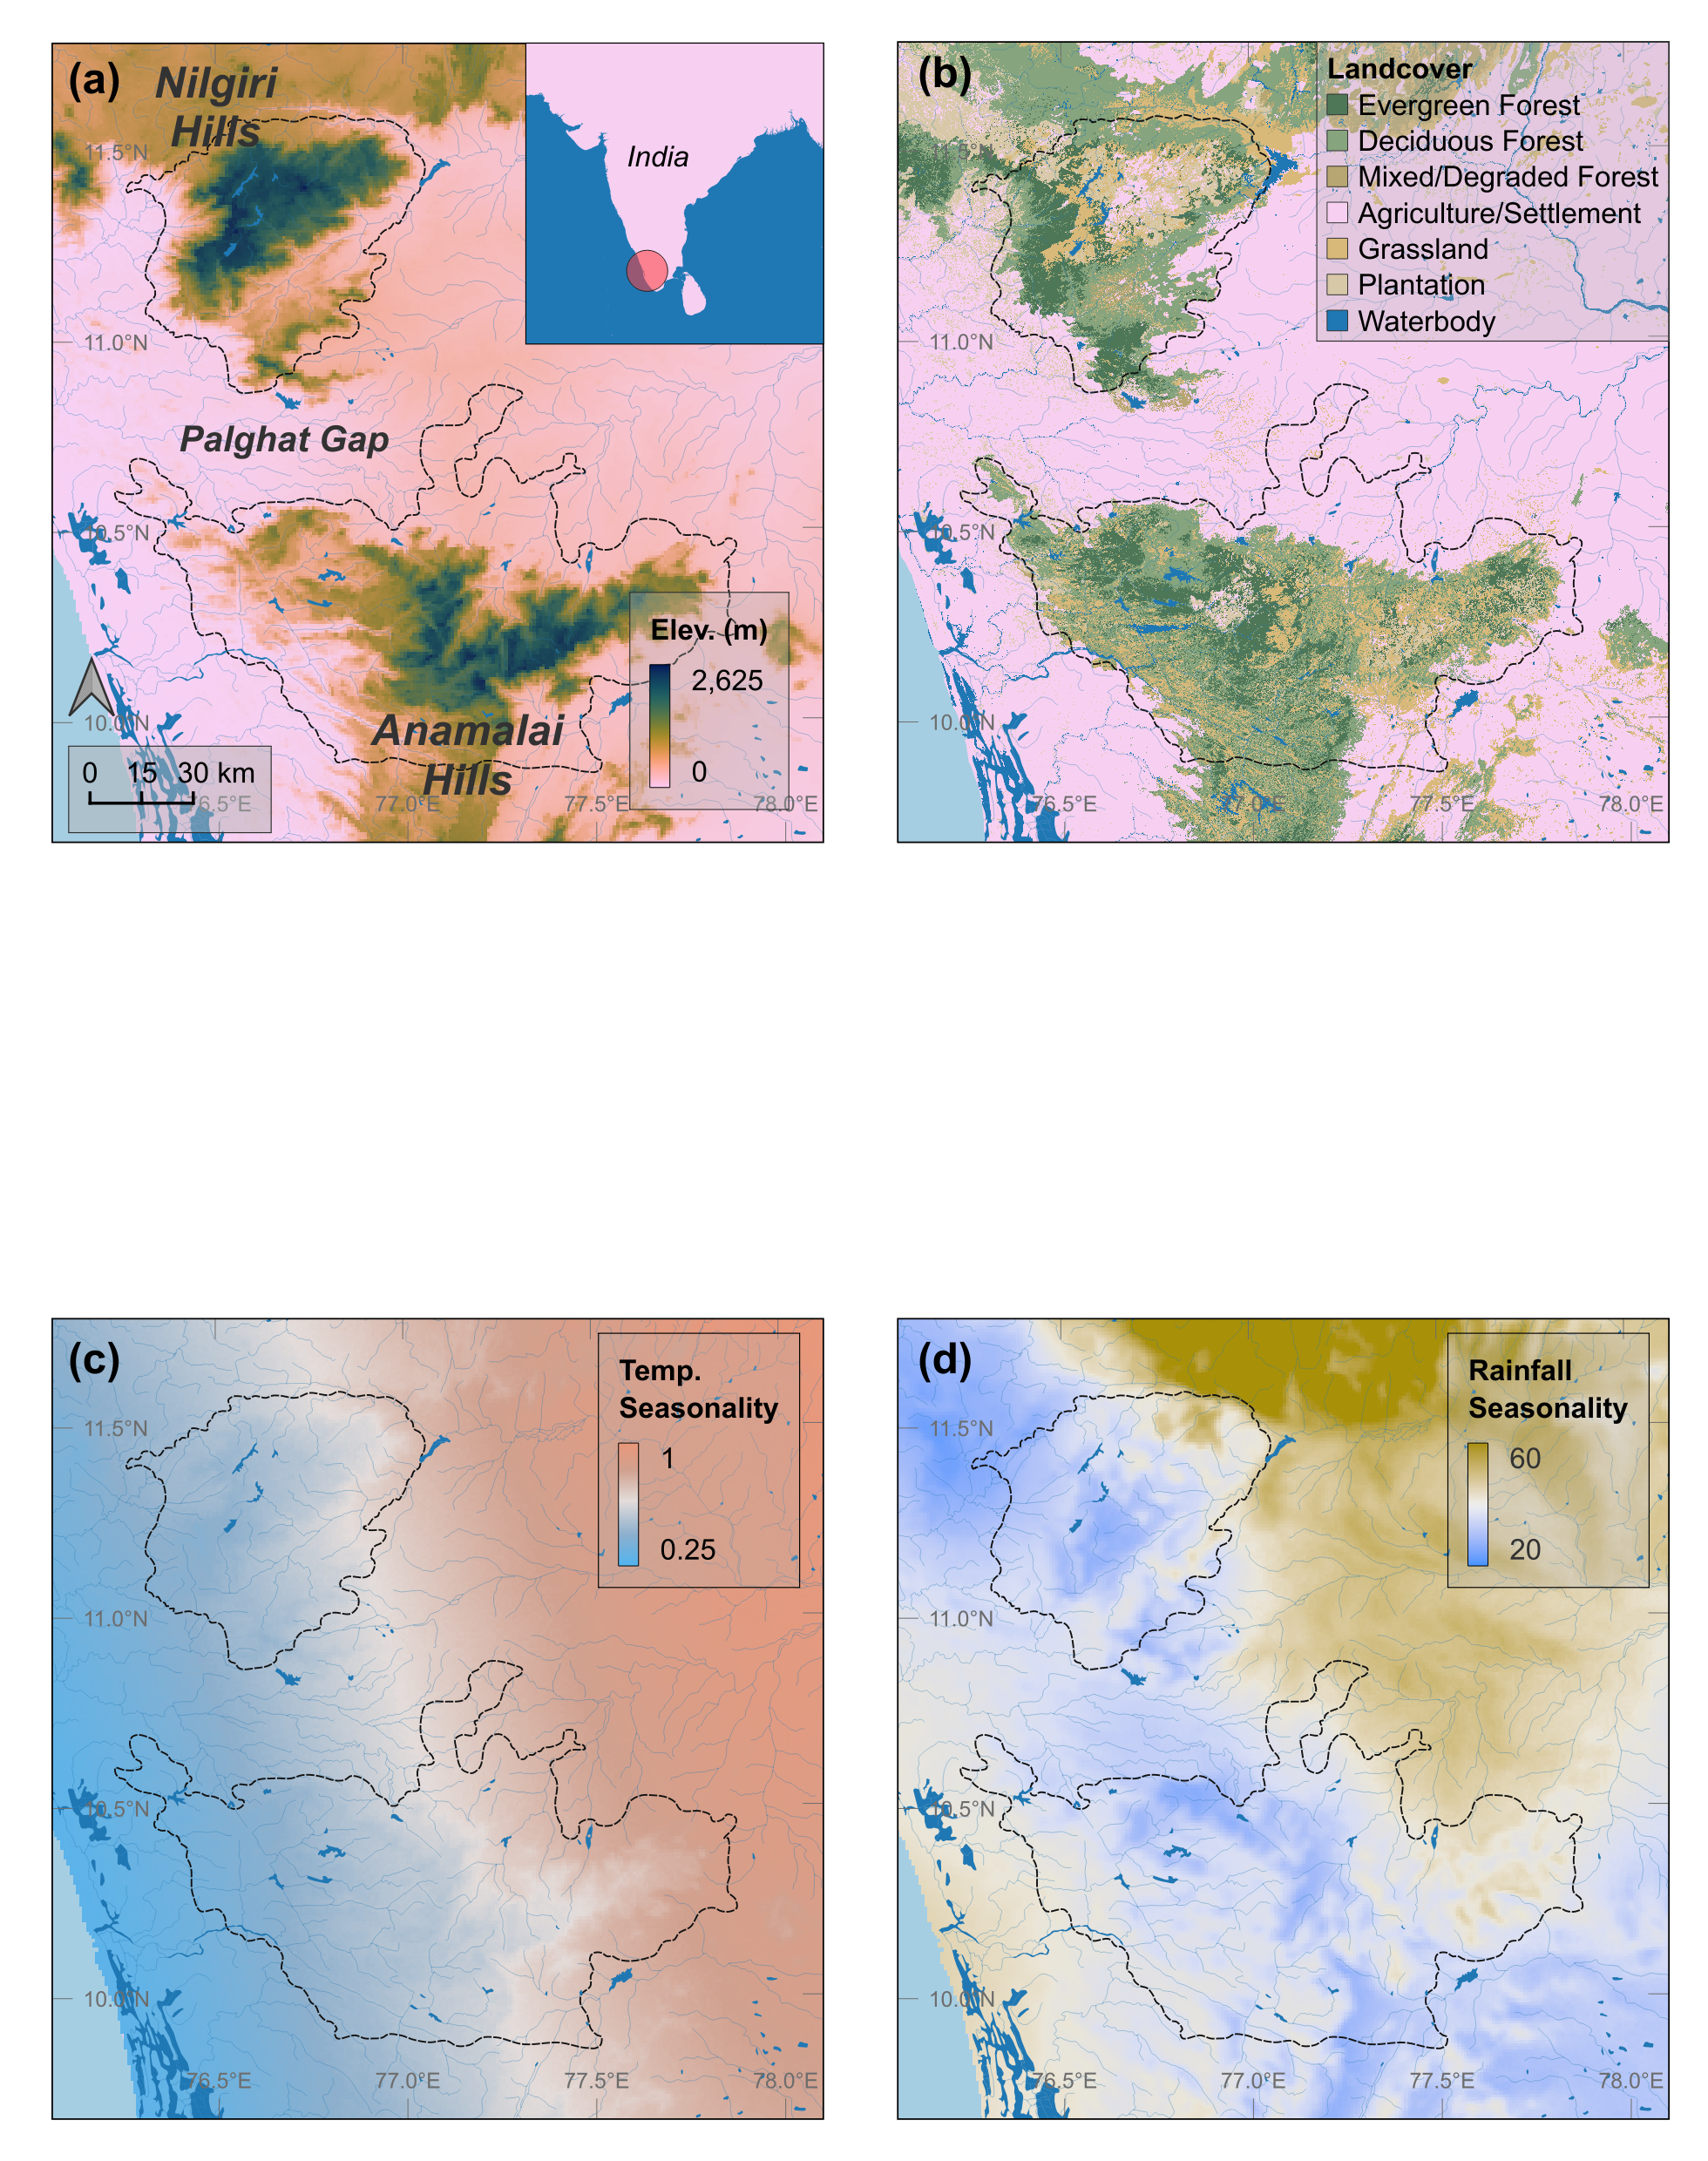
\includegraphics{figs/fig_01.png}
\caption{\textbf{The Nilgiri and Anamalai Hills in southern India provide a convenient geography for studying the interplay of land cover and climate on the distributions of bird species.}
(a) The Nilgiri and Anamalai Hills of the Southern Western Ghats are topographically complex, with maximum elevations \textgreater{} 2,000 m, and are separated by the very low-lying Palghat Gap, which serves as a natural barrier to the dispersal of many hill birds. (b) Lower elevations are primarily covered by agriculture and settlements, reflecting the intense human pressure on this region, while mid- and higher elevations show a mix of natural and human-modified land cover types (see Fig. 2 for details). (c) The coastal edge of the area, and the windward hill slopes show limited temperature seasonality across the December -- May period; this seasonality increases with distance from the coast but is lower at higher elevations inland. (d) Higher elevations also show limited precipitation seasonality than both low-lying coastal and inland regions. Our study area (bounds shown as dashed lines) includes multiple combinations of elevation, land cover type, and temperature and rainfall seasonality, resulting in a naturally occurring crossed-factorial design that allows us to study the effects of climate and land cover on bird occupancy. Representative forest-restricted and habitat-generalist birds from the study area are shown between panels (all images were obtained from Wikimedia commons and credit is assigned for each species in brackets); From L to R: (1) Malabar grey hornbill (by Koshy), (2) Crimson-backed sunbird (by Mandar Godbole), (3) Asian emerald dove (by Selvaganesh), (4) Black-and-orange flycatcher (by LKanth), (5) Grey-headed canary flycatcher (by David Raju), (6) Greater-racket tailed drongo (by MD Shahanshah Bappy), (7) Eurasian hoopoe (by Zeynel cebeci), (8) Chestnut-headed bee-eater (by MikeBirds), (9) Coppersmith barbet (by Raju Kasambe), (10) Red-vented bulbul (by TR Shankar Raman), (11) Pied bushchat (by TR Shankar Raman), (12) Ashy prinia (by Rison Thumboor). Elevation is from 30 m resolution SRTM data (Farr et al.~2007), land cover, at 1 km resolution, is reclassified from Roy et al.~(2015), while climatic variation is represented by CHELSA seasonality layers (temperature: BIOCLIM 4a, rainfall: BIOCLIM 15), at 1km resolution (Karger et al.~2017). All layers were resampled to 1 km resolution for analyses.}
\end{figure}

\hypertarget{selecting-species-of-interest}{%
\section{Selecting species of interest}\label{selecting-species-of-interest}}

Prior to preparing eBird data for occupancy modeling, we selected a list of species using a simple and objective criteria. Our primary focus is to understand how terrestrial bird species occupancy (largely passerine species) varied as a function of climate and land cover across the Nilgiri and the Anamalai hills of the Western Ghats.

We derived this list from inclusion criteria adapted from the State of India's Birds 2020 (Viswanathan et al. \protect\hyperlink{ref-viswanathan2020}{2020}). Initially, we considered all species reported on eBird that occurred within the outlines of our study area. We then added a filter to consider only terrestrial birds and removed species that are often easily confused for their congeners (eg. green/greenish warbler). In addition, we considered only those species that had a minimum of 1000 detections each between 2013 and 2021. Next, the study area was divided into 25 x 25 km cells following Viswanathan et al.~(2020). We then kept only those species that occurred in at least 5\% of all checklists across half of the 25 x 25 km cells from where they have been reported (there are 42 unique 25 x 25 km grid cells across our study area). We used the above criteria to ensure as much uniform sampling of a species as possible across our study area and to reduce any erroneous associations between environmental drivers and species occupancy. This resulted in a total of 79 species, prior to occupancy modeling.

This script shows the proportion of checklists that report a particular species across every 25km by 25km grid across the Nilgiris and the Anamalais. Using this analysis, we arrived at a final list of species for occupancy modeling.

\hypertarget{prepare-libraries}{%
\subsection{Prepare libraries}\label{prepare-libraries}}

\begin{Shaded}
\begin{Highlighting}[]
\CommentTok{# load libraries}
\KeywordTok{library}\NormalTok{(data.table)}
\KeywordTok{library}\NormalTok{(readxl)}
\KeywordTok{library}\NormalTok{(magrittr)}
\KeywordTok{library}\NormalTok{(stringr)}
\KeywordTok{library}\NormalTok{(dplyr)}
\KeywordTok{library}\NormalTok{(tidyr)}
\KeywordTok{library}\NormalTok{(readr)}
\KeywordTok{library}\NormalTok{(ggplot2)}
\KeywordTok{library}\NormalTok{(ggthemes)}
\KeywordTok{library}\NormalTok{(scico)}
\CommentTok{# round any function}
\NormalTok{round_any <-}\StringTok{ }\ControlFlowTok{function}\NormalTok{(x, }\DataTypeTok{accuracy =} \DecValTok{25000}\NormalTok{) \{}
  \KeywordTok{round}\NormalTok{(x }\OperatorTok{/}\StringTok{ }\NormalTok{accuracy) }\OperatorTok{*}\StringTok{ }\NormalTok{accuracy}
\NormalTok{\}}

\CommentTok{# set file paths for auk functions}
\CommentTok{# To use these two datasets, please download the latest versions from https://ebird.org/data/download and set the file path accordingly. Since these two datasets are extremely large, we have not uploaded the same to github.}
\CommentTok{# In this study, the version of data loaded corresponds to November 2021.}

\NormalTok{f_in_ebd <-}\StringTok{ }\KeywordTok{file.path}\NormalTok{(}\StringTok{"data/ebd_IN_relNov-2021.txt"}\NormalTok{)}
\NormalTok{f_in_sampling <-}\StringTok{ }\KeywordTok{file.path}\NormalTok{(}\StringTok{"data/ebd_sampling_relNov-2021.txt"}\NormalTok{)}
\end{Highlighting}
\end{Shaded}

\hypertarget{subset-species-by-geographical-confines-of-the-study-area}{%
\subsection{Subset species by geographical confines of the study area}\label{subset-species-by-geographical-confines-of-the-study-area}}

\begin{Shaded}
\begin{Highlighting}[]
\CommentTok{# read in shapefile of the study area to subset by bounding box}
\KeywordTok{library}\NormalTok{(sf)}
\NormalTok{wg <-}\StringTok{ }\KeywordTok{st_read}\NormalTok{(}\StringTok{"data/spatial/hillsShapefile/Nil_Ana_Pal.shp"}\NormalTok{)}
\NormalTok{box <-}\StringTok{ }\KeywordTok{st_bbox}\NormalTok{(wg)}
\CommentTok{# read in data and subset}
\CommentTok{# To access the latest dataset, please visit: https://ebird.org/data/download and set the file path accordingly.}
\NormalTok{ebd <-}\StringTok{ }\KeywordTok{fread}\NormalTok{(}\StringTok{"data/ebd_IN_relNov-2021.txt"}\NormalTok{)}
\NormalTok{ebd <-}\StringTok{ }\NormalTok{ebd[}\KeywordTok{between}\NormalTok{(LONGITUDE, box[}\StringTok{"xmin"}\NormalTok{], box[}\StringTok{"xmax"}\NormalTok{]) }\OperatorTok{&}
\StringTok{  }\KeywordTok{between}\NormalTok{(LATITUDE, box[}\StringTok{"ymin"}\NormalTok{], box[}\StringTok{"ymax"}\NormalTok{]), ]}
\NormalTok{ebd <-}\StringTok{ }\NormalTok{ebd[}\KeywordTok{year}\NormalTok{(}\StringTok{`}\DataTypeTok{OBSERVATION DATE}\StringTok{`}\NormalTok{) }\OperatorTok{>=}\StringTok{ }\DecValTok{2013}\NormalTok{, ]}
\CommentTok{# make new column names}
\NormalTok{newNames <-}\StringTok{ }\KeywordTok{str_replace_all}\NormalTok{(}\KeywordTok{colnames}\NormalTok{(ebd), }\StringTok{" "}\NormalTok{, }\StringTok{"_"}\NormalTok{) }\OperatorTok
\StringTok{  }\KeywordTok{str_to_lower}\NormalTok{()}
\KeywordTok{setnames}\NormalTok{(ebd, newNames)}
\CommentTok{# keep useful columns}
\NormalTok{columnsOfInterest <-}\StringTok{ }\KeywordTok{c}\NormalTok{(}
  \StringTok{"common_name"}\NormalTok{, }\StringTok{"scientific_name"}\NormalTok{, }\StringTok{"observation_count"}\NormalTok{, }\StringTok{"locality"}\NormalTok{,}
  \StringTok{"locality_id"}\NormalTok{, }\StringTok{"locality_type"}\NormalTok{, }\StringTok{"latitude"}\NormalTok{,}
  \StringTok{"longitude"}\NormalTok{, }\StringTok{"observation_date"}\NormalTok{, }\StringTok{"sampling_event_identifier"}
\NormalTok{)}
\NormalTok{ebd <-}\StringTok{ }\NormalTok{ebd[, ..columnsOfInterest]}
\end{Highlighting}
\end{Shaded}

\hypertarget{subset-an-initial-list-of-terrestrial-birds-based-on-a-minimum-of-1000-detections-between-2013-2021-and-b-remove-species-that-are-often-easily-confused-with-congeners}{%
\subsection{Subset an initial list of terrestrial birds based on a) minimum of 1000 detections between 2013-2021 and b) remove species that are often easily confused with congeners}\label{subset-an-initial-list-of-terrestrial-birds-based-on-a-minimum-of-1000-detections-between-2013-2021-and-b-remove-species-that-are-often-easily-confused-with-congeners}}

\begin{Shaded}
\begin{Highlighting}[]
\CommentTok{# Convert all presences marked 'X' as '1'}
\NormalTok{ebd <-}\StringTok{ }\NormalTok{ebd }\OperatorTok
\StringTok{  }\KeywordTok{mutate}\NormalTok{(}\DataTypeTok{observation_count =} \KeywordTok{ifelse}\NormalTok{(observation_count }\OperatorTok{==}\StringTok{ "X"}\NormalTok{,}
    \StringTok{"1"}\NormalTok{, observation_count}
\NormalTok{  ))}

\CommentTok{# Convert observation count to numeric}
\NormalTok{ebd}\OperatorTok{$}\NormalTok{observation_count <-}\StringTok{ }\KeywordTok{as.numeric}\NormalTok{(ebd}\OperatorTok{$}\NormalTok{observation_count)}

\NormalTok{totCount <-}\StringTok{ }\NormalTok{ebd }\OperatorTok
\StringTok{  }\NormalTok{dplyr}\OperatorTok{::}\KeywordTok{select}\NormalTok{(scientific_name, common_name, observation_count) }\OperatorTok
\StringTok{  }\KeywordTok{group_by}\NormalTok{(scientific_name, common_name) }\OperatorTok
\StringTok{  }\KeywordTok{summarise}\NormalTok{(}\DataTypeTok{tot =} \KeywordTok{sum}\NormalTok{(observation_count))}

\CommentTok{# subset species with a min of 1000 detections}
\NormalTok{tot1000 <-}\StringTok{ }\NormalTok{totCount }\OperatorTok
\StringTok{  }\KeywordTok{filter}\NormalTok{(tot }\OperatorTok{>}\StringTok{ }\DecValTok{1000}\NormalTok{)}

\NormalTok{species1000 <-}\StringTok{ }\NormalTok{tot1000}\OperatorTok{$}\NormalTok{scientific_name}

\NormalTok{ebd1000 <-}\StringTok{ }\NormalTok{ebd[scientific_name }\OperatorTok\StringTok{ }\NormalTok{species1000, ]}

\CommentTok{# Beginning with 3.37 million observations of 684 species in eBird that occurred within the outlines of our study area (Fig. 1), over the years 2013–2021, we retained only those species that had a minimum of 1,000 detections each between 2013 and 2021 (347 species remaining; 3.33 million observations). Next, we divided the study area into 25x25 km cells following State of India’s Birds 2020 methodology. We kept only those species that occurred in at least 5% of all checklists across half of the grids (42 unique grid cells) from which they had been reported. }

\CommentTok{# export the above list as .csv to carry out initial filtering based on natural history}
\KeywordTok{write.csv}\NormalTok{(totCount, }\StringTok{"data/species_list.csv"}\NormalTok{, }\DataTypeTok{row.names =}\NormalTok{ F)}
\end{Highlighting}
\end{Shaded}

\hypertarget{read-subset-of-species-following-filtering-and-removal-of-waterbirds-raptors-and-other-noctural-species}{%
\subsection{Read subset of species following filtering and removal of waterbirds, raptors, and other noctural species}\label{read-subset-of-species-following-filtering-and-removal-of-waterbirds-raptors-and-other-noctural-species}}

\begin{Shaded}
\begin{Highlighting}[]
\CommentTok{# add species of interest}
\CommentTok{# please note the below is obtained after manual subsetting based on natural history}
\NormalTok{specieslist <-}\StringTok{ }\KeywordTok{read.csv}\NormalTok{(}\StringTok{"data/species_list.csv"}\NormalTok{)}
\NormalTok{speciesOfInterest <-}\StringTok{ }\NormalTok{specieslist}\OperatorTok{$}\NormalTok{scientific_name}
\end{Highlighting}
\end{Shaded}

\hypertarget{load-raw-data-for-locations}{%
\subsection{Load raw data for locations}\label{load-raw-data-for-locations}}

Add a spatial filter and assign grids of 25km x 25km.

\begin{Shaded}
\begin{Highlighting}[]
\CommentTok{# strict spatial filter and assign grid}
\NormalTok{locs <-}\StringTok{ }\NormalTok{ebd[, .(longitude, latitude)]}
\CommentTok{# transform to UTM and get 25km boxes}
\NormalTok{coords <-}\StringTok{ }\KeywordTok{setDF}\NormalTok{(locs) }\OperatorTok
\StringTok{  }\KeywordTok{st_as_sf}\NormalTok{(}\DataTypeTok{coords =} \KeywordTok{c}\NormalTok{(}\StringTok{"longitude"}\NormalTok{, }\StringTok{"latitude"}\NormalTok{)) }\OperatorTok
\StringTok{  `}\DataTypeTok{st_crs<-}\StringTok{`}\NormalTok{(}\DecValTok{4326}\NormalTok{) }\OperatorTok
\StringTok{  }\KeywordTok{bind_cols}\NormalTok{(}\KeywordTok{as.data.table}\NormalTok{(}\KeywordTok{st_coordinates}\NormalTok{(.))) }\OperatorTok
\StringTok{  }\KeywordTok{st_transform}\NormalTok{(}\DecValTok{32643}\NormalTok{) }\OperatorTok
\StringTok{  }\KeywordTok{mutate}\NormalTok{(}\DataTypeTok{id =} \DecValTok{1}\OperatorTok{:}\KeywordTok{nrow}\NormalTok{(.))}
\CommentTok{# convert wg to UTM for filter}
\NormalTok{wg <-}\StringTok{ }\KeywordTok{st_transform}\NormalTok{(wg, }\DecValTok{32643}\NormalTok{)}
\NormalTok{coords <-}\StringTok{ }\NormalTok{coords }\OperatorTok
\StringTok{  }\KeywordTok{filter}\NormalTok{(id }\OperatorTok\StringTok{ }\KeywordTok{unlist}\NormalTok{(}\KeywordTok{st_contains}\NormalTok{(wg, coords))) }\OperatorTok
\StringTok{  }\KeywordTok{rename}\NormalTok{(}\DataTypeTok{longitude =}\NormalTok{ X, }\DataTypeTok{latitude =}\NormalTok{ Y) }\OperatorTok
\StringTok{  }\KeywordTok{bind_cols}\NormalTok{(}\KeywordTok{as.data.table}\NormalTok{(}\KeywordTok{st_coordinates}\NormalTok{(.))) }\OperatorTok
\StringTok{  }\KeywordTok{st_drop_geometry}\NormalTok{() }\OperatorTok
\StringTok{  }\KeywordTok{as.data.table}\NormalTok{()}
\CommentTok{# remove unneeded objects}
\KeywordTok{rm}\NormalTok{(locs)}
\KeywordTok{gc}\NormalTok{()}
\NormalTok{coords <-}\StringTok{ }\NormalTok{coords[, .N, by =}\StringTok{ }\NormalTok{.(longitude, latitude, X, Y)]}
\NormalTok{ebd <-}\StringTok{ }\KeywordTok{merge}\NormalTok{(ebd, coords, }\DataTypeTok{all =} \OtherTok{FALSE}\NormalTok{, }\DataTypeTok{by =} \KeywordTok{c}\NormalTok{(}\StringTok{"longitude"}\NormalTok{, }\StringTok{"latitude"}\NormalTok{))}
\NormalTok{ebd <-}\StringTok{ }\NormalTok{ebd[(longitude }\OperatorTok\StringTok{ }\NormalTok{coords}\OperatorTok{$}\NormalTok{longitude) }\OperatorTok{&}
\StringTok{  }\NormalTok{(latitude }\OperatorTok\StringTok{ }\NormalTok{coords}\OperatorTok{$}\NormalTok{latitude), ]}
\end{Highlighting}
\end{Shaded}

\hypertarget{get-proportional-obs-counts-in-25km-cells}{%
\subsection{Get proportional obs counts in 25km cells}\label{get-proportional-obs-counts-in-25km-cells}}

\begin{Shaded}
\begin{Highlighting}[]
\CommentTok{# round to 25km cell in UTM coords}
\NormalTok{ebd[, }\StringTok{`}\DataTypeTok{:=}\StringTok{`}\NormalTok{(}\DataTypeTok{X =} \KeywordTok{round_any}\NormalTok{(X), }\DataTypeTok{Y =} \KeywordTok{round_any}\NormalTok{(Y))]}
\CommentTok{# count checklists in cell}
\NormalTok{ebd_summary <-}\StringTok{ }\NormalTok{ebd[, nchk }\OperatorTok{:}\ErrorTok{=}\StringTok{ }\KeywordTok{length}\NormalTok{(}\KeywordTok{unique}\NormalTok{(sampling_event_identifier)),}
\NormalTok{  by =}\StringTok{ }\NormalTok{.(X, Y)}
\NormalTok{]}
\CommentTok{# count checklists reporting each species in cell and get proportion}
\NormalTok{ebd_summary <-}\StringTok{ }\NormalTok{ebd_summary[, .(}\DataTypeTok{nrep =} \KeywordTok{length}\NormalTok{(}\KeywordTok{unique}\NormalTok{(}
\NormalTok{  sampling_event_identifier}
\NormalTok{))),}
\NormalTok{by =}\StringTok{ }\NormalTok{.(X, Y, nchk, scientific_name)}
\NormalTok{]}
\NormalTok{ebd_summary[, p_rep }\OperatorTok{:}\ErrorTok{=}\StringTok{ }\NormalTok{nrep }\OperatorTok{/}\StringTok{ }\NormalTok{nchk]}
\CommentTok{# filter for soi}
\NormalTok{ebd_summary <-}\StringTok{ }\NormalTok{ebd_summary[scientific_name }\OperatorTok\StringTok{ }\NormalTok{speciesOfInterest, ]}
\CommentTok{# complete the dataframe for no reports}
\CommentTok{# keep no reports as NA --- allows filtering based on proportion reporting}
\NormalTok{ebd_summary <-}\StringTok{ }\KeywordTok{setDF}\NormalTok{(ebd_summary) }\OperatorTok
\StringTok{  }\KeywordTok{complete}\NormalTok{(}
    \KeywordTok{nesting}\NormalTok{(X, Y), scientific_name }\CommentTok{# ,}
    \CommentTok{# fill = list(p_rep = 0)}
\NormalTok{  ) }\OperatorTok
\StringTok{  }\KeywordTok{filter}\NormalTok{(}\OperatorTok{!}\KeywordTok{is.na}\NormalTok{(p_rep))}
\end{Highlighting}
\end{Shaded}

\hypertarget{which-species-are-reported-sufficiently-in-checklists}{%
\subsection{Which species are reported sufficiently in checklists?}\label{which-species-are-reported-sufficiently-in-checklists}}

\begin{Shaded}
\begin{Highlighting}[]
\CommentTok{# A total of 42 unique grids (of 25km by 25km) across the study area}
\CommentTok{# total number of checklists across unique grids}
\NormalTok{tot_n_chklist <-}\StringTok{ }\NormalTok{ebd_summary }\OperatorTok
\StringTok{  }\KeywordTok{distinct}\NormalTok{(X, Y, nchk)}
\CommentTok{# species-specific number of grids}
\NormalTok{spp_grids <-}\StringTok{ }\NormalTok{ebd_summary }\OperatorTok
\StringTok{  }\KeywordTok{group_by}\NormalTok{(scientific_name) }\OperatorTok
\StringTok{  }\KeywordTok{distinct}\NormalTok{(X, Y) }\OperatorTok
\StringTok{  }\KeywordTok{count}\NormalTok{(scientific_name,}
    \DataTypeTok{name =} \StringTok{"n_grids"}
\NormalTok{  )}
\CommentTok{# Write the above two results}
\KeywordTok{write_csv}\NormalTok{(tot_n_chklist, }\StringTok{"data/01_nchk_per_grid.csv"}\NormalTok{)}
\KeywordTok{write_csv}\NormalTok{(spp_grids, }\StringTok{"data/01_ngrids_per_spp.csv"}\NormalTok{)}

\CommentTok{# left-join the datasets}
\NormalTok{ebd_summary <-}\StringTok{ }\KeywordTok{left_join}\NormalTok{(ebd_summary, spp_grids, }\DataTypeTok{by =} \StringTok{"scientific_name"}\NormalTok{)}
\CommentTok{# check the proportion of grids across which this cut-off is met for each species}
\CommentTok{# Is it > 90% or 70%?}
\CommentTok{# For example, with a 3% cut-off, ~100 species are occurring in >50%}
\CommentTok{# of the grids they have been reported in}
\NormalTok{p_cutoff <-}\StringTok{ }\FloatTok{0.05} \CommentTok{# Proportion of checklists a species has been reported in}
\NormalTok{grid_proportions <-}\StringTok{ }\NormalTok{ebd_summary }\OperatorTok
\StringTok{  }\KeywordTok{group_by}\NormalTok{(scientific_name) }\OperatorTok
\StringTok{  }\KeywordTok{tally}\NormalTok{(p_rep }\OperatorTok{>=}\StringTok{ }\NormalTok{p_cutoff) }\OperatorTok
\StringTok{  }\KeywordTok{mutate}\NormalTok{(}\DataTypeTok{prop_grids_cut =}\NormalTok{ n }\OperatorTok{/}\StringTok{ }\NormalTok{(spp_grids}\OperatorTok{$}\NormalTok{n_grids)) }\OperatorTok
\StringTok{  }\KeywordTok{arrange}\NormalTok{(}\KeywordTok{desc}\NormalTok{(prop_grids_cut))}
\NormalTok{grid_prop_cut <-}\StringTok{ }\KeywordTok{filter}\NormalTok{(}
\NormalTok{  grid_proportions,}
\NormalTok{  prop_grids_cut }\OperatorTok{>=}\StringTok{ }\NormalTok{p_cutoff}
\NormalTok{)}
\CommentTok{# Write the results}
\KeywordTok{write_csv}\NormalTok{(grid_prop_cut, }\StringTok{"data/01_chk_5_percent.csv"}\NormalTok{)}

\CommentTok{# Identifying the number of species that occur in potentially <5% of all lists}
\NormalTok{total_number_lists <-}\StringTok{ }\KeywordTok{sum}\NormalTok{(tot_n_chklist}\OperatorTok{$}\NormalTok{nchk)}
\NormalTok{spp_sum_chk <-}\StringTok{ }\NormalTok{ebd_summary }\OperatorTok
\StringTok{  }\KeywordTok{distinct}\NormalTok{(X, Y, scientific_name, nrep) }\OperatorTok
\StringTok{  }\KeywordTok{group_by}\NormalTok{(scientific_name) }\OperatorTok
\StringTok{  }\KeywordTok{mutate}\NormalTok{(}\DataTypeTok{sum_chk =} \KeywordTok{sum}\NormalTok{(nrep)) }\OperatorTok
\StringTok{  }\KeywordTok{distinct}\NormalTok{(scientific_name, sum_chk)}
\CommentTok{# Approximately 90 to 100 species occur in >5% of all checklists}
\NormalTok{prop_all_lists <-}\StringTok{ }\NormalTok{spp_sum_chk }\OperatorTok
\StringTok{  }\KeywordTok{mutate}\NormalTok{(}\DataTypeTok{prop_lists =}\NormalTok{ sum_chk }\OperatorTok{/}\StringTok{ }\NormalTok{total_number_lists) }\OperatorTok
\StringTok{  }\KeywordTok{arrange}\NormalTok{(}\KeywordTok{desc}\NormalTok{(prop_lists))}
\end{Highlighting}
\end{Shaded}

\hypertarget{figure-checklist-distribution}{%
\subsection{Figure: Checklist distribution}\label{figure-checklist-distribution}}

\begin{Shaded}
\begin{Highlighting}[]
\CommentTok{# add land}
\KeywordTok{library}\NormalTok{(rnaturalearth)}
\NormalTok{land <-}\StringTok{ }\KeywordTok{ne_countries}\NormalTok{(}
  \DataTypeTok{scale =} \DecValTok{50}\NormalTok{, }\DataTypeTok{type =} \StringTok{"countries"}\NormalTok{, }\DataTypeTok{continent =} \StringTok{"asia"}\NormalTok{,}
  \DataTypeTok{country =} \StringTok{"india"}\NormalTok{,}
  \DataTypeTok{returnclass =} \KeywordTok{c}\NormalTok{(}\StringTok{"sf"}\NormalTok{)}
\NormalTok{)}
\CommentTok{# crop land}
\NormalTok{land <-}\StringTok{ }\KeywordTok{st_transform}\NormalTok{(land, }\DecValTok{32643}\NormalTok{)}
\end{Highlighting}
\end{Shaded}

\begin{figure}
\centering
\includegraphics{figs/fig_species_prop_checklists_25kmgrids.png}
\caption{Proportion of checklists reporting a species in each grid cell (25km side) between 2013 and 2021. Checklists were filtered to be within the boundaries of the Nilgiris and the Anamalai hills (black outline), but rounding to 25km cells may place cells outside the boundary. Deeper shades of red indicate a higher proportion of checklists reporting a species.}
\end{figure}

\hypertarget{prepare-the-species-list}{%
\subsection{Prepare the species list}\label{prepare-the-species-list}}

\begin{Shaded}
\begin{Highlighting}[]
\CommentTok{# write the new list of species that occur in at least 5% of checklists across a minimum of 50% of the grids they have been reported in}
\NormalTok{new_sp_list <-}\StringTok{ }\KeywordTok{semi_join}\NormalTok{(specieslist, grid_prop_cut, }\DataTypeTok{by =} \StringTok{"scientific_name"}\NormalTok{)}
\KeywordTok{write_csv}\NormalTok{(new_sp_list, }\StringTok{"data/01_list-of-species-cutoff.csv"}\NormalTok{)}
\end{Highlighting}
\end{Shaded}

\hypertarget{preparing-ebird-data}{%
\section{Preparing eBird Data}\label{preparing-ebird-data}}

\hypertarget{prepare-libraries-and-data-sources}{%
\subsection{Prepare libraries and data sources}\label{prepare-libraries-and-data-sources}}

Here, we will load the necessary libraries required for preparing the eBird data. Please download the latest versions of the eBird Basic Dataset (for India) and the eBird Sampling dataset from \url{https://ebird.org/data/download}.

\begin{Shaded}
\begin{Highlighting}[]
\CommentTok{# load libraries}
\KeywordTok{library}\NormalTok{(tidyverse)}
\KeywordTok{library}\NormalTok{(readr)}
\KeywordTok{library}\NormalTok{(sf)}
\KeywordTok{library}\NormalTok{(auk)}
\KeywordTok{library}\NormalTok{(readxl)}
\KeywordTok{library}\NormalTok{(lubridate)}

\CommentTok{# custom sum function}
\NormalTok{sum.no.na <-}\StringTok{ }\ControlFlowTok{function}\NormalTok{(x) \{}
  \KeywordTok{sum}\NormalTok{(x, }\DataTypeTok{na.rm =}\NormalTok{ T)}
\NormalTok{\}}

\CommentTok{# set file paths for auk functions}
\CommentTok{# To use these two datasets, please download the latest versions from https://ebird.org/data/download and set the file path accordingly. Since these two datasets are extremely large, we have not uploaded the same on github.}
\CommentTok{# In this study, the version of data loaded corresponds to November 2021.}

\NormalTok{f_in_ebd <-}\StringTok{ }\KeywordTok{file.path}\NormalTok{(}\StringTok{"data/ebd_IN_relNov-2021.txt"}\NormalTok{)}
\NormalTok{f_in_sampling <-}\StringTok{ }\KeywordTok{file.path}\NormalTok{(}\StringTok{"data/ebd_sampling_relNov-2021.txt"}\NormalTok{)}
\end{Highlighting}
\end{Shaded}

\hypertarget{filter-data}{%
\subsection{Filter data}\label{filter-data}}

Insert the list of species that we will be analyzing in this study. We initially chose those species that occurred in at least 5\% of all checklists across 50\% of the 25 x 25 km cells from where they have been reported, resulting in a total of 79 species. To arrive at this final list of species, we carried out further pre-processing which can be found in the previous script.

For further details regarding the list of species, please refer to the main text of the manuscript.

\begin{Shaded}
\begin{Highlighting}[]
\CommentTok{# add species of interest}
\NormalTok{specieslist <-}\StringTok{ }\KeywordTok{read.csv}\NormalTok{(}\StringTok{"data/species_list.csv"}\NormalTok{)}
\NormalTok{speciesOfInterest <-}\StringTok{ }\KeywordTok{as.character}\NormalTok{(specieslist}\OperatorTok{$}\NormalTok{scientific_name)}
\end{Highlighting}
\end{Shaded}

Here, we set broad spatial filters for the states of Kerala, Tamil Nadu and Karnataka and keep only those checklists for our list of species that were reported between 1st Jan 2013 and 31st May 2021.

\begin{Shaded}
\begin{Highlighting}[]
\CommentTok{# run filters using auk packages}
\NormalTok{ebd_filters <-}\StringTok{ }\KeywordTok{auk_ebd}\NormalTok{(f_in_ebd, f_in_sampling) }\OperatorTok
\StringTok{  }\KeywordTok{auk_species}\NormalTok{(speciesOfInterest) }\OperatorTok
\StringTok{  }\KeywordTok{auk_country}\NormalTok{(}\DataTypeTok{country =} \StringTok{"IN"}\NormalTok{) }\OperatorTok
\StringTok{  }\KeywordTok{auk_state}\NormalTok{(}\KeywordTok{c}\NormalTok{(}\StringTok{"IN-KL"}\NormalTok{, }\StringTok{"IN-TN"}\NormalTok{, }\StringTok{"IN-KA"}\NormalTok{)) }\OperatorTok
\StringTok{  }\CommentTok{# Restricting geography to TamilNadu, Kerala & Karnataka}
\StringTok{  }\KeywordTok{auk_date}\NormalTok{(}\KeywordTok{c}\NormalTok{(}\StringTok{"2013-01-01"}\NormalTok{, }\StringTok{"2021-05-31"}\NormalTok{)) }\OperatorTok
\StringTok{  }\KeywordTok{auk_complete}\NormalTok{()}

\CommentTok{# check filters}
\NormalTok{ebd_filters}
\end{Highlighting}
\end{Shaded}

Below code need not be run if it has been filtered once already and the above path leads to the right dataset. NB: This is a computation heavy process, run with caution.

\begin{Shaded}
\begin{Highlighting}[]
\CommentTok{# specify output location and perform filter}
\NormalTok{f_out_ebd <-}\StringTok{ "data/01_ebird-filtered-EBD-westernGhats.txt"}
\NormalTok{f_out_sampling <-}\StringTok{ "data/01_ebird-filtered-sampling-westernGhats.txt"}
\end{Highlighting}
\end{Shaded}

\begin{Shaded}
\begin{Highlighting}[]
\NormalTok{ebd_filtered <-}\StringTok{ }\KeywordTok{auk_filter}\NormalTok{(ebd_filters,}
  \DataTypeTok{file =}\NormalTok{ f_out_ebd,}
  \DataTypeTok{file_sampling =}\NormalTok{ f_out_sampling, }\DataTypeTok{overwrite =} \OtherTok{TRUE}
\NormalTok{)}
\end{Highlighting}
\end{Shaded}

\hypertarget{process-filtered-data}{%
\subsection{Process filtered data}\label{process-filtered-data}}

The data has been filtered above using the auk functions. We will now work with the filtered checklist observations (Please note that we have not yet spatially filtered the checklists to the confines of our study area, which is the Nilgiris and the Anamalai hills. This step is carried out further on).

\begin{Shaded}
\begin{Highlighting}[]
\CommentTok{# read in the data}
\NormalTok{ebd <-}\StringTok{ }\KeywordTok{read_ebd}\NormalTok{(f_out_ebd)}
\end{Highlighting}
\end{Shaded}

eBird checklists only suggest whether a species was reported at a particular location. To arrive at absence data, we use a process known as zero-filling (Johnston et al. \protect\hyperlink{ref-johnston2019a}{2019}), wherein a new dataframe is created with a 0 marked for each checklist when the bird was not observed.

\begin{Shaded}
\begin{Highlighting}[]
\CommentTok{# fill zeroes}
\NormalTok{zf <-}\StringTok{ }\KeywordTok{auk_zerofill}\NormalTok{(f_out_ebd, f_out_sampling)}
\NormalTok{new_zf <-}\StringTok{ }\KeywordTok{collapse_zerofill}\NormalTok{(zf)}
\end{Highlighting}
\end{Shaded}

Let us now choose specific columns necessary for further analysis.

\begin{Shaded}
\begin{Highlighting}[]
\CommentTok{# choose columns of interest}
\NormalTok{columnsOfInterest <-}\StringTok{ }\KeywordTok{c}\NormalTok{(}
  \StringTok{"checklist_id"}\NormalTok{, }\StringTok{"scientific_name"}\NormalTok{, }\StringTok{"common_name"}\NormalTok{,}
  \StringTok{"observation_count"}\NormalTok{, }\StringTok{"locality"}\NormalTok{, }\StringTok{"locality_id"}\NormalTok{,}
  \StringTok{"locality_type"}\NormalTok{, }\StringTok{"latitude"}\NormalTok{, }\StringTok{"longitude"}\NormalTok{,}
  \StringTok{"observation_date"}\NormalTok{, }\StringTok{"time_observations_started"}\NormalTok{,}
  \StringTok{"observer_id"}\NormalTok{, }\StringTok{"sampling_event_identifier"}\NormalTok{,}
  \StringTok{"protocol_type"}\NormalTok{, }\StringTok{"duration_minutes"}\NormalTok{,}
  \StringTok{"effort_distance_km"}\NormalTok{, }\StringTok{"effort_area_ha"}\NormalTok{,}
  \StringTok{"number_observers"}\NormalTok{, }\StringTok{"species_observed"}\NormalTok{,}
  \StringTok{"reviewed"}
\NormalTok{)}

\CommentTok{# make list of presence and absence data and choose cols of interest}
\NormalTok{data <-}\StringTok{ }\KeywordTok{list}\NormalTok{(ebd, new_zf) }\OperatorTok
\StringTok{  }\KeywordTok{map}\NormalTok{(}\ControlFlowTok{function}\NormalTok{(x) \{}
\NormalTok{    x }\OperatorTok\StringTok{ }\KeywordTok{select}\NormalTok{(}\KeywordTok{one_of}\NormalTok{(columnsOfInterest))}
\NormalTok{  \})}

\CommentTok{# remove zerofills to save working memory}
\KeywordTok{rm}\NormalTok{(zf, new_zf)}
\KeywordTok{gc}\NormalTok{()}

\CommentTok{# check for presences and absence in absences df, remove essentially the presences df which may lead to erroneous analysis}
\NormalTok{data[[}\DecValTok{2}\NormalTok{]] <-}\StringTok{ }\NormalTok{data[[}\DecValTok{2}\NormalTok{]] }\OperatorTok\StringTok{ }\KeywordTok{filter}\NormalTok{(species_observed }\OperatorTok{==}\StringTok{ }\NormalTok{F)}
\end{Highlighting}
\end{Shaded}

\hypertarget{spatial-filter}{%
\subsection{Spatial filter}\label{spatial-filter}}

A spatial filter is now supplied to further restrict our list of observations to the confines of the Nilgiris and the Anamalai hills of the Western Ghats biodiversity hotspot.

\begin{Shaded}
\begin{Highlighting}[]
\CommentTok{# load shapefile of the study area}
\KeywordTok{library}\NormalTok{(sf)}
\NormalTok{hills <-}\StringTok{ }\KeywordTok{st_read}\NormalTok{(}\StringTok{"data/spatial/hillsShapefile/Nil_Ana_Pal.shp"}\NormalTok{)}

\CommentTok{# write a prelim filter by bounding box}
\NormalTok{box <-}\StringTok{ }\KeywordTok{st_bbox}\NormalTok{(hills)}

\CommentTok{# get data spatial coordinates}
\NormalTok{dataLocs <-}\StringTok{ }\NormalTok{data }\OperatorTok
\StringTok{  }\KeywordTok{map}\NormalTok{(}\ControlFlowTok{function}\NormalTok{(x) \{}
    \KeywordTok{select}\NormalTok{(x, longitude, latitude) }\OperatorTok
\StringTok{      }\KeywordTok{filter}\NormalTok{(}\KeywordTok{between}\NormalTok{(longitude, box[}\StringTok{"xmin"}\NormalTok{], box[}\StringTok{"xmax"}\NormalTok{]) }\OperatorTok{&}
\StringTok{        }\KeywordTok{between}\NormalTok{(latitude, box[}\StringTok{"ymin"}\NormalTok{], box[}\StringTok{"ymax"}\NormalTok{]))}
\NormalTok{  \}) }\OperatorTok
\StringTok{  }\KeywordTok{bind_rows}\NormalTok{() }\OperatorTok
\StringTok{  }\KeywordTok{distinct}\NormalTok{() }\OperatorTok
\StringTok{  }\KeywordTok{st_as_sf}\NormalTok{(}\DataTypeTok{coords =} \KeywordTok{c}\NormalTok{(}\StringTok{"longitude"}\NormalTok{, }\StringTok{"latitude"}\NormalTok{)) }\OperatorTok
\StringTok{  }\KeywordTok{st_set_crs}\NormalTok{(}\DecValTok{4326}\NormalTok{) }\OperatorTok
\StringTok{  }\KeywordTok{st_intersection}\NormalTok{(hills)}

\CommentTok{# get simplified data and drop geometry}
\NormalTok{dataLocs <-}\StringTok{ }\KeywordTok{mutate}\NormalTok{(dataLocs, }\DataTypeTok{spatialKeep =}\NormalTok{ T) }\OperatorTok
\StringTok{  }\KeywordTok{bind_cols}\NormalTok{(., }\KeywordTok{as_tibble}\NormalTok{(}\KeywordTok{st_coordinates}\NormalTok{(dataLocs))) }\OperatorTok
\StringTok{  }\KeywordTok{st_drop_geometry}\NormalTok{()}

\CommentTok{# bind to data and then filter}
\NormalTok{data <-}\StringTok{ }\NormalTok{data }\OperatorTok
\StringTok{  }\KeywordTok{map}\NormalTok{(}\ControlFlowTok{function}\NormalTok{(x) \{}
    \KeywordTok{left_join}\NormalTok{(x, dataLocs, }\DataTypeTok{by =} \KeywordTok{c}\NormalTok{(}\StringTok{"longitude"}\NormalTok{ =}\StringTok{ "X"}\NormalTok{, }\StringTok{"latitude"}\NormalTok{ =}\StringTok{ "Y"}\NormalTok{)) }\OperatorTok
\StringTok{      }\KeywordTok{filter}\NormalTok{(spatialKeep }\OperatorTok{==}\StringTok{ }\NormalTok{T) }\OperatorTok
\StringTok{      }\KeywordTok{select}\NormalTok{(}\OperatorTok{-}\NormalTok{Id, }\OperatorTok{-}\NormalTok{spatialKeep)}
\NormalTok{  \})}
\end{Highlighting}
\end{Shaded}

Save temporary data created so far.

\begin{Shaded}
\begin{Highlighting}[]
\CommentTok{# save a temp data file}
\KeywordTok{save}\NormalTok{(data, }\DataTypeTok{file =} \StringTok{"data/01_data_temp.rdata"}\NormalTok{)}
\end{Highlighting}
\end{Shaded}

\hypertarget{handle-presence-data}{%
\subsection{Handle presence data}\label{handle-presence-data}}

Further pre-processing is required in the case of many checklists where species abundance is often unknown and an `X' is denoted in such cases. Here, we convert all `X' notations to a 1, suggesting a presence (as we are not concerned with abundance data in this analysis). We also removed those checklists where the duration in minutes is either not recorded or listed as zero. Lastly, we added an sampling effort based filter following (Johnston et al. \protect\hyperlink{ref-johnston2019a}{2019}), wherein we considered only those checklists with duration in minutes is less than 300 and distance in kilometers traveled is less than 5km. Lastly, we excluded those group checklists where the number of observers was greater than 10. For the sake of occupancy modeling of appropriate detection and occupancy covariates, we restrict all our checklists between December 1st and May 31st (non-rainy months)and checklists recorded between 5am and 7pm.

\begin{Shaded}
\begin{Highlighting}[]
\CommentTok{# in the first set, replace X, for presences, with 1}
\NormalTok{data[[}\DecValTok{1}\NormalTok{]] <-}\StringTok{ }\NormalTok{data[[}\DecValTok{1}\NormalTok{]] }\OperatorTok
\StringTok{  }\KeywordTok{mutate}\NormalTok{(}\DataTypeTok{observation_count =} \KeywordTok{ifelse}\NormalTok{(observation_count }\OperatorTok{==}\StringTok{ "X"}\NormalTok{,}
    \StringTok{"1"}\NormalTok{, observation_count}
\NormalTok{  ))}

\CommentTok{# remove records where duration is 0}
\NormalTok{data <-}\StringTok{ }\KeywordTok{map}\NormalTok{(data, }\ControlFlowTok{function}\NormalTok{(x) }\KeywordTok{filter}\NormalTok{(x, duration_minutes }\OperatorTok{>}\StringTok{ }\DecValTok{0}\NormalTok{))}

\CommentTok{# group data by site and sampling event identifier}
\CommentTok{# then, summarise relevant variables as the sum}
\NormalTok{dataGrouped <-}\StringTok{ }\KeywordTok{map}\NormalTok{(data, }\ControlFlowTok{function}\NormalTok{(x) \{}
\NormalTok{  x }\OperatorTok
\StringTok{    }\KeywordTok{group_by}\NormalTok{(sampling_event_identifier) }\OperatorTok
\StringTok{    }\KeywordTok{summarise_at}\NormalTok{(}
      \KeywordTok{vars}\NormalTok{(}
\NormalTok{        duration_minutes, effort_distance_km,}
\NormalTok{        effort_area_ha}
\NormalTok{      ),}
      \KeywordTok{list}\NormalTok{(sum.no.na)}
\NormalTok{    )}
\NormalTok{\})}

\CommentTok{# bind rows combining data frames, and filter}
\NormalTok{dataGrouped <-}\StringTok{ }\KeywordTok{bind_rows}\NormalTok{(dataGrouped) }\OperatorTok
\StringTok{  }\KeywordTok{filter}\NormalTok{(}
\NormalTok{    duration_minutes }\OperatorTok{<=}\StringTok{ }\DecValTok{300}\NormalTok{,}
\NormalTok{    effort_distance_km }\OperatorTok{<=}\StringTok{ }\DecValTok{5}\NormalTok{,}
\NormalTok{    effort_area_ha }\OperatorTok{<=}\StringTok{ }\DecValTok{500}
\NormalTok{  )}

\CommentTok{# get data identifiers, such as sampling identifier etc}
\NormalTok{dataConstants <-}\StringTok{ }\NormalTok{data }\OperatorTok
\StringTok{  }\KeywordTok{bind_rows}\NormalTok{() }\OperatorTok
\StringTok{  }\KeywordTok{select}\NormalTok{(}
\NormalTok{    sampling_event_identifier, time_observations_started,}
\NormalTok{    locality, locality_type, locality_id,}
\NormalTok{    observer_id, observation_date, scientific_name,}
\NormalTok{    observation_count, protocol_type, number_observers,}
\NormalTok{    longitude, latitude}
\NormalTok{  )}

\CommentTok{# join the summarised data with the identifiers,}
\CommentTok{# using sampling_event_identifier as the key}
\NormalTok{dataGrouped <-}\StringTok{ }\KeywordTok{left_join}\NormalTok{(dataGrouped, dataConstants,}
  \DataTypeTok{by =} \StringTok{"sampling_event_identifier"}
\NormalTok{)}

\CommentTok{# remove checklists or seis with more than 10 obervers}
\KeywordTok{count}\NormalTok{(dataGrouped, number_observers }\OperatorTok{>}\StringTok{ }\DecValTok{10}\NormalTok{) }\CommentTok{# count how many have 10+ obs}
\NormalTok{dataGrouped <-}\StringTok{ }\KeywordTok{filter}\NormalTok{(dataGrouped, number_observers }\OperatorTok{<=}\StringTok{ }\DecValTok{10}\NormalTok{)}

\CommentTok{# keep only checklists between 5AM and 7PM}
\NormalTok{dataGrouped <-}\StringTok{ }\KeywordTok{filter}\NormalTok{(dataGrouped, time_observations_started }\OperatorTok{>=}\StringTok{ "05:00:00"} \OperatorTok{&}\StringTok{ }\NormalTok{time_observations_started }\OperatorTok{<=}\StringTok{ "19:00:00"}\NormalTok{)}

\CommentTok{# keep only checklists between December 1st and May 31st}
\NormalTok{dataGrouped <-}\StringTok{ }\KeywordTok{filter}\NormalTok{(dataGrouped, }\KeywordTok{month}\NormalTok{(observation_date) }\OperatorTok\StringTok{ }\KeywordTok{c}\NormalTok{(}\DecValTok{1}\NormalTok{, }\DecValTok{2}\NormalTok{, }\DecValTok{3}\NormalTok{, }\DecValTok{4}\NormalTok{, }\DecValTok{5}\NormalTok{, }\DecValTok{12}\NormalTok{))}
\end{Highlighting}
\end{Shaded}

\hypertarget{add-decimal-time}{%
\subsection{Add decimal time}\label{add-decimal-time}}

We added a column where time is denoted in decimal hours since midnight.

\begin{Shaded}
\begin{Highlighting}[]
\CommentTok{# assign present or not, and get time in decimal hours since midnight}
\KeywordTok{library}\NormalTok{(lubridate)}
\NormalTok{time_to_decimal <-}\StringTok{ }\ControlFlowTok{function}\NormalTok{(x) \{}
\NormalTok{  x <-}\StringTok{ }\KeywordTok{hms}\NormalTok{(x, }\DataTypeTok{quiet =} \OtherTok{TRUE}\NormalTok{)}
  \KeywordTok{hour}\NormalTok{(x) }\OperatorTok{+}\StringTok{ }\KeywordTok{minute}\NormalTok{(x) }\OperatorTok{/}\StringTok{ }\DecValTok{60} \OperatorTok{+}\StringTok{ }\KeywordTok{second}\NormalTok{(x) }\OperatorTok{/}\StringTok{ }\DecValTok{3600}
\NormalTok{\}}

\CommentTok{# will cause issues if using time obs started as a linear effect and not quadratic}
\NormalTok{dataGrouped <-}\StringTok{ }\KeywordTok{mutate}\NormalTok{(dataGrouped,}
  \DataTypeTok{pres_abs =}\NormalTok{ observation_count }\OperatorTok{>=}\StringTok{ }\DecValTok{1}\NormalTok{,}
  \DataTypeTok{decimalTime =} \KeywordTok{time_to_decimal}\NormalTok{(time_observations_started)}
\NormalTok{)}

\CommentTok{# check class of dataGrouped, make sure not sf}
\NormalTok{assertthat}\OperatorTok{::}\KeywordTok{assert_that}\NormalTok{(}\OperatorTok{!}\StringTok{"sf"} \OperatorTok\StringTok{ }\KeywordTok{class}\NormalTok{(dataGrouped))}
\end{Highlighting}
\end{Shaded}

The above data is saved to a file.

\begin{Shaded}
\begin{Highlighting}[]
\CommentTok{# save a temp data file}
\KeywordTok{save}\NormalTok{(dataGrouped, }\DataTypeTok{file =} \StringTok{"data/01_data_prelim_processing.Rdata"}\NormalTok{)}
\end{Highlighting}
\end{Shaded}

\hypertarget{preparing-environmental-predictors}{%
\section{Preparing Environmental Predictors}\label{preparing-environmental-predictors}}

In this script, we processed climatic and landscape predictors for occupancy modeling.

All climatic data was obtained from \url{https://chelsa-climate.org/bioclim/}
All landscape data was derived from a high resolution land cover map (Roy et al.~2015). This map provides sufficient classes to achieve a high land cover resolution and can be accessed here (\url{https://daac.ornl.gov/VEGETATION/guides/Decadal_LULC_India.html})

The goal here is to resample all rasters so that they have the same resolution of 1km cells.

\hypertarget{prepare-libraries-1}{%
\subsection{Prepare libraries}\label{prepare-libraries-1}}

We load some common libraries for raster processing and define a custom mode function.

\begin{Shaded}
\begin{Highlighting}[]
\CommentTok{# load libs}
\KeywordTok{library}\NormalTok{(raster)}
\KeywordTok{library}\NormalTok{(stringi)}
\KeywordTok{library}\NormalTok{(glue)}
\KeywordTok{library}\NormalTok{(gdalUtils)}
\KeywordTok{library}\NormalTok{(purrr)}
\KeywordTok{library}\NormalTok{(dplyr)}
\KeywordTok{library}\NormalTok{(tidyr)}
\KeywordTok{library}\NormalTok{(tibble)}

\CommentTok{# for plotting}
\KeywordTok{library}\NormalTok{(viridis)}
\KeywordTok{library}\NormalTok{(colorspace)}
\KeywordTok{library}\NormalTok{(tmap)}
\KeywordTok{library}\NormalTok{(scales)}
\KeywordTok{library}\NormalTok{(ggplot2)}
\KeywordTok{library}\NormalTok{(patchwork)}

\CommentTok{# prep mode function to aggregate}
\NormalTok{funcMode <-}\StringTok{ }\ControlFlowTok{function}\NormalTok{(x, }\DataTypeTok{na.rm =}\NormalTok{ T) \{}
\NormalTok{  ux <-}\StringTok{ }\KeywordTok{unique}\NormalTok{(x)}
\NormalTok{  ux[}\KeywordTok{which.max}\NormalTok{(}\KeywordTok{tabulate}\NormalTok{(}\KeywordTok{match}\NormalTok{(x, ux)))]}
\NormalTok{\}}

\CommentTok{# a basic test}
\NormalTok{assertthat}\OperatorTok{::}\KeywordTok{assert_that}\NormalTok{(}\KeywordTok{funcMode}\NormalTok{(}\KeywordTok{c}\NormalTok{(}\DecValTok{2}\NormalTok{, }\DecValTok{2}\NormalTok{, }\DecValTok{2}\NormalTok{, }\DecValTok{2}\NormalTok{, }\DecValTok{3}\NormalTok{, }\DecValTok{3}\NormalTok{, }\DecValTok{3}\NormalTok{, }\DecValTok{4}\NormalTok{)) }\OperatorTok{==}\StringTok{ }\KeywordTok{as.character}\NormalTok{(}\DecValTok{2}\NormalTok{),}
  \DataTypeTok{msg =} \StringTok{"problem in the mode function"}
\NormalTok{) }\CommentTok{# works}

\CommentTok{# get ci func}
\NormalTok{ci <-}\StringTok{ }\ControlFlowTok{function}\NormalTok{(x) \{}
  \KeywordTok{qnorm}\NormalTok{(}\FloatTok{0.975}\NormalTok{) }\OperatorTok{*}\StringTok{ }\KeywordTok{sd}\NormalTok{(x, }\DataTypeTok{na.rm =}\NormalTok{ T) }\OperatorTok{/}\StringTok{ }\KeywordTok{sqrt}\NormalTok{(}\KeywordTok{length}\NormalTok{(x))}
\NormalTok{\}}
\end{Highlighting}
\end{Shaded}

\hypertarget{prepare-spatial-extent}{%
\subsection{Prepare spatial extent}\label{prepare-spatial-extent}}

We prepare a 30km buffer around the boundary of the study area. This buffer will be used to mask the landscape rasters.The buffer procedure is done on data transformed to the UTM 43N CRS to avoid distortions.

\begin{Shaded}
\begin{Highlighting}[]
\CommentTok{# load hills}
\KeywordTok{library}\NormalTok{(sf)}
\NormalTok{hills <-}\StringTok{ }\KeywordTok{st_read}\NormalTok{(}\StringTok{"data/spatial/hillsShapefile/Nil_Ana_Pal.shp"}\NormalTok{)}
\NormalTok{hills <-}\StringTok{ }\KeywordTok{st_transform}\NormalTok{(hills, }\DecValTok{32643}\NormalTok{)}
\NormalTok{buffer <-}\StringTok{ }\KeywordTok{st_buffer}\NormalTok{(hills, }\FloatTok{3e4}\NormalTok{) }\OperatorTok
\StringTok{  }\KeywordTok{st_transform}\NormalTok{(}\DecValTok{4326}\NormalTok{)}
\end{Highlighting}
\end{Shaded}

\hypertarget{prepare-terrain-rasters}{%
\subsection{Prepare terrain rasters}\label{prepare-terrain-rasters}}

We prepare the elevation data which is an SRTM raster layer, and derive the slope and aspect from it after cropping it to the extent of the study site buffer. Please download the latest version of the SRTM raster layer from \url{https://www.worldclim.org/data/worldclim21.html}

\begin{Shaded}
\begin{Highlighting}[]
\CommentTok{# load elevation and crop to hills size, then mask by study area}
\NormalTok{alt <-}\StringTok{ }\KeywordTok{raster}\NormalTok{(}\StringTok{"data/spatial/Elevation/alt"}\NormalTok{) }\CommentTok{# this layer is not added to github as a result of its large size and can be downloaded from the above link}
\NormalTok{alt.hills <-}\StringTok{ }\NormalTok{raster}\OperatorTok{::}\KeywordTok{crop}\NormalTok{(alt, }\KeywordTok{as}\NormalTok{(buffer, }\StringTok{"Spatial"}\NormalTok{))}
\KeywordTok{rm}\NormalTok{(alt)}
\KeywordTok{gc}\NormalTok{()}

\CommentTok{# get slope and aspect}
\NormalTok{slopeData <-}\StringTok{ }\NormalTok{raster}\OperatorTok{::}\KeywordTok{terrain}\NormalTok{(}\DataTypeTok{x =}\NormalTok{ alt.hills, }\DataTypeTok{opt =} \KeywordTok{c}\NormalTok{(}\StringTok{"slope"}\NormalTok{, }\StringTok{"aspect"}\NormalTok{))}
\NormalTok{elevData <-}\StringTok{ }\NormalTok{raster}\OperatorTok{::}\KeywordTok{stack}\NormalTok{(alt.hills, slopeData)}
\KeywordTok{rm}\NormalTok{(alt.hills)}
\KeywordTok{gc}\NormalTok{()}
\end{Highlighting}
\end{Shaded}

\hypertarget{prepare-chelsa-rasters}{%
\subsection{Prepare CHELSA rasters}\label{prepare-chelsa-rasters}}

CHELSA rasters can be downloaded using the \texttt{get\_chelsa.sh} shell script, which is a \texttt{wget} command pointing to the \texttt{envidatS3.txt} file.

\hypertarget{prepare-bioclim-4a-and-15}{%
\subsubsection{Prepare BIOCLIM 4a and 15}\label{prepare-bioclim-4a-and-15}}

We prepare the CHELSA rasters for seasonality in temperature (Bio 4a) and seasonality in precipitation (Bio 15) in the same way, reading them in, cropping them to the study site buffer extent, and handling the temperature layer values which we divide by 10. The CHELSA rasters can be downloaded from \url{https://chelsa-climate.org/bioclim/}

\begin{Shaded}
\begin{Highlighting}[]
\CommentTok{# list chelsa files}
\CommentTok{# the chelsa data can be downloaded from the aforementioned link. They haven't been uploaded to github as a result of its large size.}
\NormalTok{chelsaFiles <-}\StringTok{ }\KeywordTok{list.files}\NormalTok{(}\StringTok{"data/chelsa/"}\NormalTok{,}
  \DataTypeTok{full.names =} \OtherTok{TRUE}\NormalTok{,}
  \DataTypeTok{recursive =} \OtherTok{TRUE}\NormalTok{,}
  \DataTypeTok{pattern =} \StringTok{"bio10"}
\NormalTok{)}

\CommentTok{# gather chelsa rasters}
\NormalTok{chelsaData <-}\StringTok{ }\NormalTok{purrr}\OperatorTok{::}\KeywordTok{map}\NormalTok{(chelsaFiles, }\ControlFlowTok{function}\NormalTok{(chr) \{}
\NormalTok{  a <-}\StringTok{ }\KeywordTok{raster}\NormalTok{(chr)}
  \KeywordTok{crs}\NormalTok{(a) <-}\StringTok{ }\KeywordTok{crs}\NormalTok{(elevData)}
\NormalTok{  a <-}\StringTok{ }\KeywordTok{crop}\NormalTok{(a, }\KeywordTok{as}\NormalTok{(buffer, }\StringTok{"Spatial"}\NormalTok{))}
  \KeywordTok{return}\NormalTok{(a)}
\NormalTok{\})}

\CommentTok{# divide temperature by 10}
\NormalTok{chelsaData[[}\DecValTok{1}\NormalTok{]] <-}\StringTok{ }\NormalTok{chelsaData[[}\DecValTok{1}\NormalTok{]] }\OperatorTok{/}\StringTok{ }\DecValTok{10}

\CommentTok{# stack chelsa data}
\NormalTok{chelsaData <-}\StringTok{ }\NormalTok{raster}\OperatorTok{::}\KeywordTok{stack}\NormalTok{(chelsaData)}
\end{Highlighting}
\end{Shaded}

\hypertarget{prepare-bioclim-4a}{%
\subsubsection{Prepare BIOCLIM 4a}\label{prepare-bioclim-4a}}

\begin{Shaded}
\begin{Highlighting}[]
\ControlFlowTok{if}\NormalTok{ (}\KeywordTok{file.exists}\NormalTok{(}\StringTok{"data/chelsa/CHELSA_bio10_4a.tif"}\NormalTok{)) \{}
  \KeywordTok{message}\NormalTok{(}\StringTok{"Bio 4a already exists, will be overwritten"}\NormalTok{)}
\NormalTok{\}}
\end{Highlighting}
\end{Shaded}

Bioclim 4a, the coefficient of variation temperature seasonality is calculated as

\[Bio\ 4a = \frac{SD\{ Tkavg_1, \ldots Tkavg_{12} \}}{(Bio\ 1 + 273.15)} \times 100\]

where \(Tkavg_i = (Tkmin_i + Tkmax_i) / 2\)

Here, we use only the months of December and Jan -- May for winter temperature variation.

\begin{Shaded}
\begin{Highlighting}[]
\CommentTok{# list rasters by pattern}
\NormalTok{patterns <-}\StringTok{ }\KeywordTok{c}\NormalTok{(}\StringTok{"tmin"}\NormalTok{, }\StringTok{"tmax"}\NormalTok{)}

\CommentTok{# list the filepaths}
\NormalTok{tkAvg <-}\StringTok{ }\KeywordTok{map}\NormalTok{(patterns, }\ControlFlowTok{function}\NormalTok{(pattern) \{}
  \CommentTok{# list the paths}
\NormalTok{  files <-}\StringTok{ }\KeywordTok{list.files}\NormalTok{(}
    \DataTypeTok{path =} \StringTok{"data/chelsa"}\NormalTok{,}
    \DataTypeTok{full.names =} \OtherTok{TRUE}\NormalTok{,}
    \DataTypeTok{recursive =} \OtherTok{TRUE}\NormalTok{,}
    \DataTypeTok{pattern =}\NormalTok{ pattern}
\NormalTok{  )}
\NormalTok{\})}

\CommentTok{# print crs elev data for sanity check --- basic WGS84}
\KeywordTok{crs}\NormalTok{(elevData)}

\CommentTok{# now run over the paths and read as rasters and crop by buffer}
\NormalTok{tkAvg <-}\StringTok{ }\KeywordTok{map}\NormalTok{(tkAvg, }\ControlFlowTok{function}\NormalTok{(paths) \{}
  \CommentTok{# going over the file paths, read them in as rasters, convert CRS and crop}
\NormalTok{  tempData <-}\StringTok{ }\KeywordTok{map}\NormalTok{(paths, }\ControlFlowTok{function}\NormalTok{(path) \{}
    \CommentTok{# read in}
\NormalTok{    a <-}\StringTok{ }\KeywordTok{raster}\NormalTok{(path)}
    \CommentTok{# assign crs}
    \KeywordTok{crs}\NormalTok{(a) <-}\StringTok{ }\KeywordTok{crs}\NormalTok{(elevData)}
    \CommentTok{# crop by buffer, will throw error if CRS doesn't match}
\NormalTok{    a <-}\StringTok{ }\KeywordTok{crop}\NormalTok{(a, }\KeywordTok{as}\NormalTok{(buffer, }\StringTok{"Spatial"}\NormalTok{))}
    \CommentTok{# return a}
\NormalTok{    a}
\NormalTok{  \})}
  \CommentTok{# convert each to kelvin, first dividing by 10 to get celsius}
\NormalTok{  tempData <-}\StringTok{ }\KeywordTok{map}\NormalTok{(tempData, }\ControlFlowTok{function}\NormalTok{(tmpRaster) \{}
\NormalTok{    tmpRaster <-}\StringTok{ }\NormalTok{(tmpRaster }\OperatorTok{/}\StringTok{ }\DecValTok{10}\NormalTok{) }\OperatorTok{+}\StringTok{ }\FloatTok{273.15}
\NormalTok{  \})}
\NormalTok{\})}

\CommentTok{# assign names}
\KeywordTok{names}\NormalTok{(tkAvg) <-}\StringTok{ }\NormalTok{patterns}

\CommentTok{# go over the tmin and tmax and get the average monthly temp}
\NormalTok{tkAvg <-}\StringTok{ }\KeywordTok{map2}\NormalTok{(tkAvg[[}\StringTok{"tmin"}\NormalTok{]], tkAvg[[}\StringTok{"tmax"}\NormalTok{]], }\ControlFlowTok{function}\NormalTok{(tmin, tmax) \{}
  \CommentTok{# return the mean of the corresponding tmin and tmax}
  \CommentTok{# still in kelvin}
  \KeywordTok{calc}\NormalTok{(}\KeywordTok{stack}\NormalTok{(tmin, tmax), }\DataTypeTok{fun =}\NormalTok{ mean)}
\NormalTok{\})}

\CommentTok{# calculate Bio 4a}
\NormalTok{bio_4a <-}\StringTok{ }\NormalTok{(}\KeywordTok{calc}\NormalTok{(}\KeywordTok{stack}\NormalTok{(tkAvg), }\DataTypeTok{fun =}\NormalTok{ sd) }\OperatorTok{/}\StringTok{ }\NormalTok{(chelsaData[[}\DecValTok{1}\NormalTok{]] }\OperatorTok{+}\StringTok{ }\FloatTok{273.15}\NormalTok{)) }\OperatorTok{*}\StringTok{ }\DecValTok{100}
\KeywordTok{names}\NormalTok{(bio_4a) <-}\StringTok{ "CHELSA_bio10_4a"}
\CommentTok{# save bio_4a}
\KeywordTok{writeRaster}\NormalTok{(bio_4a, }\DataTypeTok{filename =} \StringTok{"data/chelsa/CHELSA_bio10_4a.tif"}\NormalTok{, }\DataTypeTok{overwrite =}\NormalTok{ T)}
\end{Highlighting}
\end{Shaded}

\hypertarget{prepare-bioclim-15}{%
\subsubsection{Prepare Bioclim 15}\label{prepare-bioclim-15}}

\begin{Shaded}
\begin{Highlighting}[]
\ControlFlowTok{if}\NormalTok{ (}\KeywordTok{file.exists}\NormalTok{(}\StringTok{"data/chelsa/CHELSA_bio10_15.tif"}\NormalTok{)) \{}
  \KeywordTok{message}\NormalTok{(}\StringTok{"Bio 15 already exists, will be overwritten"}\NormalTok{)}
\NormalTok{\}}
\end{Highlighting}
\end{Shaded}

Bioclim 15, the coefficient of variation precipitation (in our area, rainfall) seasonality is calculated as

\[Bio\ 15 = \frac{SD\{ PPT_1, \ldots PPT_{12} \}}{1 + (Bio\ 12 / 12)} \times 100\]

where \(PPT_i\) is the monthly precipitation.

Here, we use only the months of December and Jan -- May for winter rainfall variation.

\begin{Shaded}
\begin{Highlighting}[]
\CommentTok{# list rasters by pattern}
\NormalTok{pattern <-}\StringTok{ "prec"}

\CommentTok{# list the filepaths}
\NormalTok{pptTotal <-}\StringTok{ }\KeywordTok{list.files}\NormalTok{(}
  \DataTypeTok{path =} \StringTok{"data/chelsa"}\NormalTok{,}
  \DataTypeTok{full.names =} \OtherTok{TRUE}\NormalTok{,}
  \DataTypeTok{recursive =} \OtherTok{TRUE}\NormalTok{,}
  \DataTypeTok{pattern =}\NormalTok{ pattern}
\NormalTok{)}

\CommentTok{# print crs elev data for sanity check --- basic WGS84}
\KeywordTok{crs}\NormalTok{(elevData)}

\CommentTok{# now run over the paths and read as rasters and crop by buffer}
\NormalTok{pptTotal <-}\StringTok{ }\KeywordTok{map}\NormalTok{(pptTotal, }\ControlFlowTok{function}\NormalTok{(path) \{}
\NormalTok{  a <-}\StringTok{ }\KeywordTok{raster}\NormalTok{(path)}
  \CommentTok{# assign crs}
  \KeywordTok{crs}\NormalTok{(a) <-}\StringTok{ }\KeywordTok{crs}\NormalTok{(elevData)}
  \CommentTok{# crop by buffer, will throw error if CRS doesn't match}
\NormalTok{  a <-}\StringTok{ }\KeywordTok{crop}\NormalTok{(a, }\KeywordTok{as}\NormalTok{(buffer, }\StringTok{"Spatial"}\NormalTok{))}
  \CommentTok{# return a}
\NormalTok{  a}
\NormalTok{\})}

\CommentTok{# calculate Bio 4a}
\NormalTok{bio_}\DecValTok{15}\NormalTok{ <-}\StringTok{ }\NormalTok{(}\KeywordTok{calc}\NormalTok{(}\KeywordTok{stack}\NormalTok{(pptTotal), }\DataTypeTok{fun =}\NormalTok{ sd) }\OperatorTok{/}\StringTok{ }\NormalTok{(}\DecValTok{1} \OperatorTok{+}\StringTok{ }\NormalTok{(chelsaData[[}\DecValTok{2}\NormalTok{]] }\OperatorTok{/}\StringTok{ }\DecValTok{12}\NormalTok{))) }\OperatorTok{*}\StringTok{ }\DecValTok{100}
\KeywordTok{names}\NormalTok{(bio_}\DecValTok{15}\NormalTok{) <-}\StringTok{ "CHELSA_bio10_15"}
\CommentTok{# save bio_4a}
\KeywordTok{writeRaster}\NormalTok{(bio_}\DecValTok{15}\NormalTok{, }\DataTypeTok{filename =} \StringTok{"data/chelsa/CHELSA_bio10_15.tif"}\NormalTok{, }\DataTypeTok{overwrite =}\NormalTok{ T)}
\end{Highlighting}
\end{Shaded}

\hypertarget{stack-terrain-and-climate}{%
\subsubsection{Stack terrain and climate}\label{stack-terrain-and-climate}}

We stack the terrain and climatic rasters.

\begin{Shaded}
\begin{Highlighting}[]
\CommentTok{# If bio4a and bio15 have already been prepared from previous runs/analysis - load them directly}
\NormalTok{bio_4a <-}\StringTok{ }\KeywordTok{raster}\NormalTok{(}\StringTok{"data/chelsa/CHELSA_bio10_4a.tif"}\NormalTok{)}
\NormalTok{bio_}\DecValTok{15}\NormalTok{ <-}\StringTok{ }\KeywordTok{raster}\NormalTok{(}\StringTok{"data/chelsa/CHELSA_bio10_15.tif"}\NormalTok{)}
\end{Highlighting}
\end{Shaded}

\hypertarget{stack-terrain-and-climate-1}{%
\subsubsection{Stack terrain and climate}\label{stack-terrain-and-climate-1}}

We stack the terrain and climatic rasters.

\begin{Shaded}
\begin{Highlighting}[]
\CommentTok{# stack rasters for efficient reprojection later}
\NormalTok{env_data <-}\StringTok{ }\KeywordTok{stack}\NormalTok{(elevData, bio_4a, bio_}\DecValTok{15}\NormalTok{)}
\end{Highlighting}
\end{Shaded}

\hypertarget{resample-landcover-from-10m-to-1km}{%
\subsection{Resample landcover from 10m to 1km}\label{resample-landcover-from-10m-to-1km}}

We read in a land cover classified image and resample that using the mode function to a 1km resolution. Please note that the resampling process need not be carried out as it has been done already and the resampled raster can be loaded with the subsequent code chunk.

\begin{Shaded}
\begin{Highlighting}[]
\CommentTok{# read in landcover raster location}
\CommentTok{# To access the land cover data, please visit: https://daac.ornl.gov/VEGETATION/guides/Decadal_LULC_India.html}

\NormalTok{landcover <-}\StringTok{ "data/landUseClassification/landcover_roy_2015/"}

\CommentTok{# read in and crop}
\NormalTok{landcover <-}\StringTok{ }\KeywordTok{raster}\NormalTok{(landcover)}
\NormalTok{buffer_utm <-}\StringTok{ }\KeywordTok{st_transform}\NormalTok{(buffer, }\DecValTok{32643}\NormalTok{)}
\NormalTok{landcover <-}\StringTok{ }\KeywordTok{crop}\NormalTok{(}
\NormalTok{  landcover,}
  \KeywordTok{as}\NormalTok{(}
\NormalTok{    buffer_utm,}
    \StringTok{"Spatial"}
\NormalTok{  )}
\NormalTok{)}

\CommentTok{# read reclassification matrix}
\NormalTok{reclassification_matrix <-}\StringTok{ }\KeywordTok{read.csv}\NormalTok{(}\StringTok{"data/landUseClassification/LandCover_ReclassifyMatrix_2015.csv"}\NormalTok{)}
\NormalTok{reclassification_matrix <-}\StringTok{ }\KeywordTok{as.matrix}\NormalTok{(reclassification_matrix[, }\KeywordTok{c}\NormalTok{(}\StringTok{"V1"}\NormalTok{, }\StringTok{"To"}\NormalTok{)])}

\CommentTok{# reclassify}
\NormalTok{landcover_reclassified <-}\StringTok{ }\KeywordTok{reclassify}\NormalTok{(}
  \DataTypeTok{x =}\NormalTok{ landcover,}
  \DataTypeTok{rcl =}\NormalTok{ reclassification_matrix}
\NormalTok{)}

\CommentTok{# write to file}
\KeywordTok{writeRaster}\NormalTok{(landcover_reclassified,}
  \DataTypeTok{filename =} \StringTok{"data/landUseClassification/landcover_roy_2015_reclassified.tif"}\NormalTok{,}
  \DataTypeTok{overwrite =} \OtherTok{TRUE}
\NormalTok{)}

\CommentTok{# check reclassification}
\KeywordTok{plot}\NormalTok{(landcover_reclassified)}

\CommentTok{# get extent}
\NormalTok{e <-}\StringTok{ }\KeywordTok{bbox}\NormalTok{(}\KeywordTok{raster}\NormalTok{(landcover))}

\CommentTok{# init resolution}
\NormalTok{res_init <-}\StringTok{ }\KeywordTok{res}\NormalTok{(}\KeywordTok{raster}\NormalTok{(landcover))}

\CommentTok{# res to transform to 1000m}
\NormalTok{res_final <-}\StringTok{ }\NormalTok{res_init }\OperatorTok{*}\StringTok{ }\NormalTok{(}\DecValTok{1000} \OperatorTok{/}\StringTok{ }\NormalTok{res_init)}

\CommentTok{# use gdalutils gdalwarp for resampling transform}
\CommentTok{# to 1km from 10m}
\NormalTok{gdalUtils}\OperatorTok{::}\KeywordTok{gdalwarp}\NormalTok{(}
  \DataTypeTok{srcfile =} \StringTok{"data/landUseClassification/landcover_roy_2015_reclassified.tif"}\NormalTok{,}
  \DataTypeTok{dstfile =} \StringTok{"data/landUseClassification/lc_01000m.tif"}\NormalTok{,}
  \DataTypeTok{tr =} \KeywordTok{c}\NormalTok{(res_final), }\DataTypeTok{r =} \StringTok{"mode"}\NormalTok{, }\DataTypeTok{te =} \KeywordTok{c}\NormalTok{(e)}
\NormalTok{)}
\end{Highlighting}
\end{Shaded}

We compare the frequency of landcover classes between the original raster and the resampled 1km raster to be certain that the resampling has not resulted in drastic misrepresentation of the frequency of any landcover type. This comparison is made using the figure below.

\begin{figure}
\centering
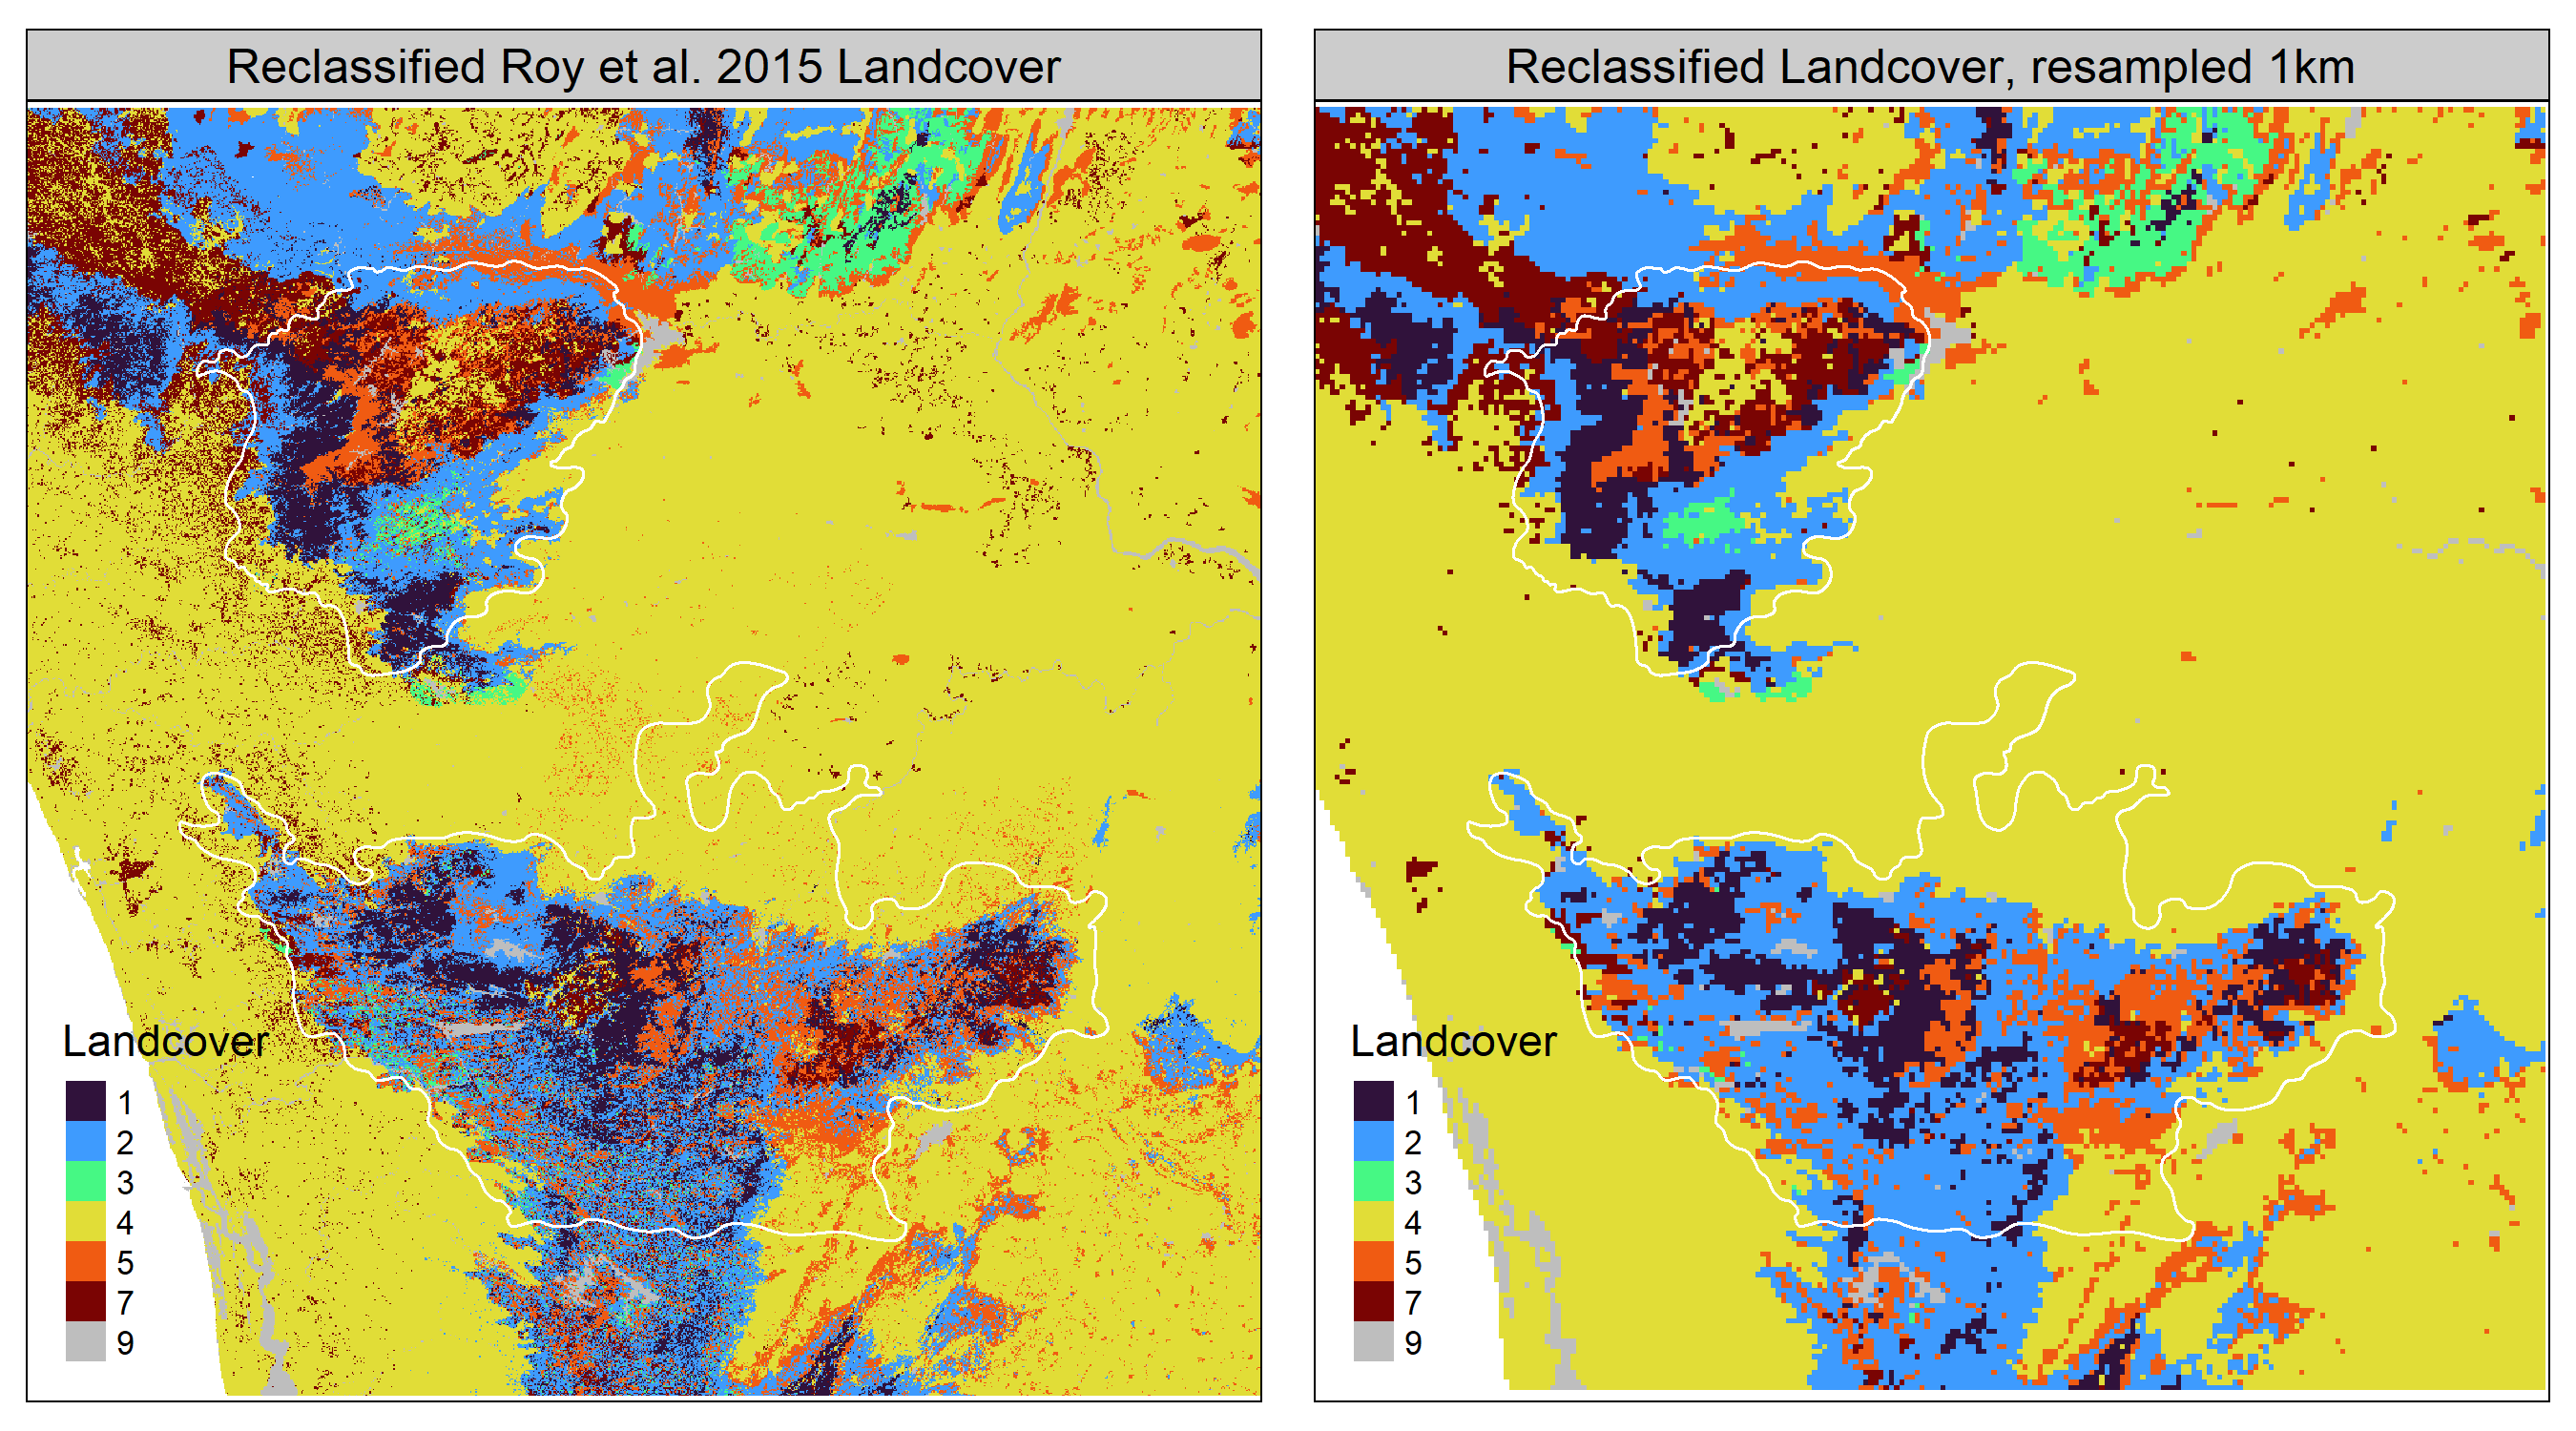
\includegraphics{figs/fig_landcover_resample.png}
\caption{Resampling the Roy et al.~(2015) landcover raster, reclassified into 7 main classes, to a resolution of 1km, preserves the important features of landcover over the study area.}
\end{figure}

\hypertarget{resample-other-rasters-to-1km}{%
\subsection{Resample other rasters to 1km}\label{resample-other-rasters-to-1km}}

We now resample all other rasters to a resolution of 1km.

\hypertarget{read-in-resampled-landcover}{%
\subsubsection{Read in resampled landcover}\label{read-in-resampled-landcover}}

Here, we read in the 1km landcover raster and set 0 to NA.

\begin{Shaded}
\begin{Highlighting}[]
\NormalTok{lc_data <-}\StringTok{ }\KeywordTok{raster}\NormalTok{(}\StringTok{"data/landUseClassification/lc_01000m.tif"}\NormalTok{)}
\NormalTok{lc_data[lc_data }\OperatorTok{==}\StringTok{ }\DecValTok{0}\NormalTok{] <-}\StringTok{ }\OtherTok{NA}
\end{Highlighting}
\end{Shaded}

\hypertarget{reproject-environmental-data-using-landcover-as-a-template}{%
\subsubsection{Reproject environmental data using landcover as a template}\label{reproject-environmental-data-using-landcover-as-a-template}}

\begin{Shaded}
\begin{Highlighting}[]
\CommentTok{# resample to the corresponding landcover data}
\NormalTok{env_data_resamp <-}\StringTok{ }\KeywordTok{projectRaster}\NormalTok{(}
  \DataTypeTok{from =}\NormalTok{ env_data, }\DataTypeTok{to =}\NormalTok{ lc_data,}
  \DataTypeTok{crs =} \KeywordTok{crs}\NormalTok{(lc_data), }\DataTypeTok{res =} \KeywordTok{res}\NormalTok{(lc_data)}
\NormalTok{)}

\CommentTok{# export as raster stack}
\NormalTok{land_stack <-}\StringTok{ }\KeywordTok{stack}\NormalTok{(env_data_resamp, lc_data)}

\CommentTok{# get names}
\NormalTok{land_names <-}\StringTok{ }\KeywordTok{glue}\NormalTok{(}\StringTok{'data/spatial/landscape_resamp\{c("01")\}_km.tif'}\NormalTok{)}

\CommentTok{# write to file}
\NormalTok{raster}\OperatorTok{::}\KeywordTok{writeRaster}\NormalTok{(}
\NormalTok{  land_stack, }\DataTypeTok{filename =} \KeywordTok{as.character}\NormalTok{(land_names), }
  \DataTypeTok{overwrite =} \OtherTok{TRUE}
\NormalTok{)}
\end{Highlighting}
\end{Shaded}

\hypertarget{climate-variables-in-relation-to-elevation}{%
\subsection{Climate variables in relation to elevation}\label{climate-variables-in-relation-to-elevation}}

\hypertarget{load-resampled-environmental-rasters}{%
\subsubsection{Load resampled environmental rasters}\label{load-resampled-environmental-rasters}}

\begin{Shaded}
\begin{Highlighting}[]
\CommentTok{# read landscape prepare for plotting}
\NormalTok{landscape <-}\StringTok{ }\KeywordTok{stack}\NormalTok{(}\StringTok{"data/spatial/landscape_resamp01_km.tif"}\NormalTok{)}

\CommentTok{# get proper names}
\NormalTok{elev_names <-}\StringTok{ }\KeywordTok{c}\NormalTok{(}\StringTok{"elev"}\NormalTok{, }\StringTok{"slope"}\NormalTok{, }\StringTok{"aspect"}\NormalTok{)}
\NormalTok{chelsa_names <-}\StringTok{ }\KeywordTok{c}\NormalTok{(}\StringTok{"bio_4a"}\NormalTok{, }\StringTok{"bio_15"}\NormalTok{)}

\KeywordTok{names}\NormalTok{(landscape) <-}\StringTok{ }\KeywordTok{glue}\NormalTok{(}\StringTok{'\{c(elev_names, chelsa_names, "landcover")\}'}\NormalTok{)}
\end{Highlighting}
\end{Shaded}

\begin{Shaded}
\begin{Highlighting}[]
\CommentTok{# make duplicate stack}
\NormalTok{land_data <-}\StringTok{ }\NormalTok{landscape[[}\KeywordTok{c}\NormalTok{(}\StringTok{"elev"}\NormalTok{, chelsa_names)]]}

\CommentTok{# convert to list}
\NormalTok{land_data <-}\StringTok{ }\KeywordTok{as.list}\NormalTok{(land_data)}

\CommentTok{# map get values over the stack}
\NormalTok{land_data <-}\StringTok{ }\NormalTok{purrr}\OperatorTok{::}\KeywordTok{map}\NormalTok{(land_data, getValues)}
\KeywordTok{names}\NormalTok{(land_data) <-}\StringTok{ }\KeywordTok{c}\NormalTok{(}\StringTok{"elev"}\NormalTok{, chelsa_names)}

\CommentTok{# conver to dataframe and round to 200m}
\NormalTok{land_data <-}\StringTok{ }\KeywordTok{bind_cols}\NormalTok{(land_data)}
\NormalTok{land_data <-}\StringTok{ }\KeywordTok{drop_na}\NormalTok{(land_data) }\OperatorTok
\StringTok{  }\KeywordTok{mutate}\NormalTok{(}\DataTypeTok{elev_round =}\NormalTok{ plyr}\OperatorTok{::}\KeywordTok{round_any}\NormalTok{(elev, }\DecValTok{200}\NormalTok{)) }\OperatorTok
\StringTok{  }\NormalTok{dplyr}\OperatorTok{::}\KeywordTok{select}\NormalTok{(}\OperatorTok{-}\NormalTok{elev) }\OperatorTok
\StringTok{  }\KeywordTok{pivot_longer}\NormalTok{(}
    \DataTypeTok{cols =} \KeywordTok{contains}\NormalTok{(}\StringTok{"bio"}\NormalTok{),}
    \DataTypeTok{names_to =} \StringTok{"clim_var"}
\NormalTok{  ) }\OperatorTok
\StringTok{  }\KeywordTok{group_by}\NormalTok{(elev_round, clim_var) }\OperatorTok
\StringTok{  }\KeywordTok{summarise_all}\NormalTok{(}\DataTypeTok{.funs =} \KeywordTok{list}\NormalTok{(}\OperatorTok{~}\StringTok{ }\KeywordTok{mean}\NormalTok{(.), }\OperatorTok{~}\StringTok{ }\KeywordTok{ci}\NormalTok{(.)))}
\end{Highlighting}
\end{Shaded}

Figure code is hidden in versions rendered as HTML or PDF.

\hypertarget{climate-across-land-cover-types}{%
\subsection{Climate across land cover types}\label{climate-across-land-cover-types}}

Get climate values per (re-classified) landcover type from the 1km resampled raster.

\begin{Shaded}
\begin{Highlighting}[]
\CommentTok{# make duplicate stack again}
\NormalTok{lc_clim_data <-}\StringTok{ }\NormalTok{landscape[[}\KeywordTok{c}\NormalTok{(}\StringTok{"landcover"}\NormalTok{, chelsa_names)]]}

\CommentTok{# convert to list}
\NormalTok{lc_clim_data <-}\StringTok{ }\KeywordTok{as.list}\NormalTok{(lc_clim_data)}

\CommentTok{# map get values over the stack}
\NormalTok{lc_clim_data <-}\StringTok{ }\NormalTok{purrr}\OperatorTok{::}\KeywordTok{map}\NormalTok{(lc_clim_data, getValues)}
\KeywordTok{names}\NormalTok{(lc_clim_data) <-}\StringTok{ }\KeywordTok{c}\NormalTok{(}\StringTok{"landcover"}\NormalTok{, chelsa_names)}

\CommentTok{# conver to dataframe for histogram}
\NormalTok{lc_clim_data <-}\StringTok{ }\KeywordTok{bind_cols}\NormalTok{(lc_clim_data)}

\CommentTok{# pivot long}
\NormalTok{lc_clim_data <-}\StringTok{ }\KeywordTok{pivot_longer}\NormalTok{(}
\NormalTok{  lc_clim_data,}
  \DataTypeTok{cols =} \KeywordTok{contains}\NormalTok{(}\StringTok{"bio"}\NormalTok{),}
  \DataTypeTok{names_to =} \StringTok{"climvar"}
\NormalTok{)}

\CommentTok{# make landcover factor}
\NormalTok{lc_clim_data <-}\StringTok{ }\KeywordTok{mutate}\NormalTok{(}
\NormalTok{  lc_clim_data,}
  \DataTypeTok{landcover =} \KeywordTok{factor}\NormalTok{(landcover)}
\NormalTok{)}

\CommentTok{# filter bio }
\NormalTok{lc_clim_data <-}\StringTok{ }\KeywordTok{filter}\NormalTok{(}
\NormalTok{  lc_clim_data,}
  \OperatorTok{!}\KeywordTok{is.na}\NormalTok{(landcover)}
\NormalTok{)}

\CommentTok{# split by variable}
\NormalTok{lc_clim_data <-}\StringTok{ }\KeywordTok{nest}\NormalTok{(lc_clim_data, }\DataTypeTok{data =} \KeywordTok{c}\NormalTok{(}\StringTok{"landcover"}\NormalTok{, }\StringTok{"value"}\NormalTok{))}

\CommentTok{# assign names}
\NormalTok{lc_clim_data}\OperatorTok{$}\NormalTok{climvar_name <-}\StringTok{ }\KeywordTok{c}\NormalTok{(}
  \StringTok{"Temperature seasonality"}\NormalTok{,}
  \StringTok{"Precipitation seasonality"}
\NormalTok{)}
\end{Highlighting}
\end{Shaded}

Plot density plots of climate seasonality per LC type.

\begin{Shaded}
\begin{Highlighting}[]
\CommentTok{# make labels}
\NormalTok{lc_labels <-}\StringTok{ }\KeywordTok{c}\NormalTok{(}
  \StringTok{"Evergreen"}\NormalTok{, }\StringTok{"Deciduous"}\NormalTok{,}
  \StringTok{"Mixed./Degr."}\NormalTok{, }\StringTok{"Agri./Settl."}\NormalTok{,}
  \StringTok{"Grassland"}\NormalTok{, }\StringTok{"Plantation"}\NormalTok{,}
  \StringTok{"Waterbody"}
\NormalTok{)}
\KeywordTok{names}\NormalTok{(lc_labels) <-}\StringTok{ }\KeywordTok{c}\NormalTok{(}\KeywordTok{seq}\NormalTok{(}\DecValTok{5}\NormalTok{), }\DecValTok{7}\NormalTok{, }\DecValTok{9}\NormalTok{)}

\CommentTok{# plots}
\NormalTok{lc_clim_plots <-}\StringTok{ }\KeywordTok{pmap}\NormalTok{(}
\NormalTok{  lc_clim_data,}
  \ControlFlowTok{function}\NormalTok{(climvar_name, data, climvar) \{}
\NormalTok{    p <-}\StringTok{ }\NormalTok{data }\OperatorTok
\StringTok{      }\KeywordTok{ggplot}\NormalTok{() }\OperatorTok{+}
\StringTok{      }\KeywordTok{geom_histogram}\NormalTok{(}
        \KeywordTok{aes}\NormalTok{(}
          \DataTypeTok{x =}\NormalTok{ value, }\DataTypeTok{y =}\NormalTok{ ..density..,}
          \DataTypeTok{fill =}\NormalTok{ ..x..}
\NormalTok{        ),}
        \DataTypeTok{show.legend =}\NormalTok{ F}
\NormalTok{      ) }\OperatorTok{+}
\StringTok{      }\KeywordTok{theme_test}\NormalTok{(}\DataTypeTok{base_family =} \StringTok{"Arial"}\NormalTok{) }\OperatorTok{+}
\StringTok{      }\KeywordTok{theme}\NormalTok{(}
        \DataTypeTok{legend.key.width =} \KeywordTok{unit}\NormalTok{(}\DecValTok{2}\NormalTok{, }\DataTypeTok{units =} \StringTok{"mm"}\NormalTok{),}
        \DataTypeTok{axis.text.y =} \KeywordTok{element_blank}\NormalTok{(),}
        \DataTypeTok{axis.text.x =} \KeywordTok{element_text}\NormalTok{(}\DataTypeTok{size =} \DecValTok{6}\NormalTok{, }\DataTypeTok{angle =} \DecValTok{45}\NormalTok{),}
        \DataTypeTok{axis.ticks.y =} \KeywordTok{element_blank}\NormalTok{(),}
        \DataTypeTok{strip.background =} \KeywordTok{element_blank}\NormalTok{(),}
        \DataTypeTok{strip.text =} \KeywordTok{element_text}\NormalTok{(}\DataTypeTok{size =} \DecValTok{6}\NormalTok{, }\DataTypeTok{face =} \StringTok{"bold"}\NormalTok{)}
\NormalTok{      ) }\OperatorTok{+}
\StringTok{      }\KeywordTok{facet_grid}\NormalTok{(}
        \OperatorTok{~}\NormalTok{landcover,}
        \DataTypeTok{labeller =} \KeywordTok{labeller}\NormalTok{(}
          \DataTypeTok{landcover =}\NormalTok{ lc_labels}
\NormalTok{        )}
\NormalTok{      ) }\OperatorTok{+}
\StringTok{      }\KeywordTok{labs}\NormalTok{(}
        \DataTypeTok{x =} \KeywordTok{glue}\NormalTok{(}\StringTok{"\{climvar_name\}"}\NormalTok{),}
        \DataTypeTok{y =} \StringTok{"Density"}
\NormalTok{      )}
    \ControlFlowTok{if}\NormalTok{ (climvar }\OperatorTok{==}\StringTok{ "bio_1"}\NormalTok{) \{}
\NormalTok{      p <-}\StringTok{ }\NormalTok{p }\OperatorTok{+}
\StringTok{        }\KeywordTok{scale_fill_continuous_diverging}\NormalTok{(}
          \DataTypeTok{palette =} \StringTok{"Blue-Red 2"}\NormalTok{,}
          \DataTypeTok{mid =} \FloatTok{29.5}
\NormalTok{        )}
\NormalTok{    \} }\ControlFlowTok{else}\NormalTok{ \{}
\NormalTok{      p <-}\StringTok{ }\NormalTok{p }\OperatorTok{+}
\StringTok{        }\KeywordTok{scale_x_continuous}\NormalTok{(}
          \DataTypeTok{limits =} \KeywordTok{c}\NormalTok{(}\DecValTok{200}\NormalTok{, }\DecValTok{500}\NormalTok{)}
\NormalTok{        ) }\OperatorTok{+}
\StringTok{        }\KeywordTok{scale_fill_continuous_diverging}\NormalTok{(}
          \DataTypeTok{palette =} \StringTok{"Blue-Yellow 2"}\NormalTok{,}
          \DataTypeTok{mid =} \DecValTok{350}
\NormalTok{        )}
\NormalTok{    \}}

\NormalTok{    p}
\NormalTok{  \}}
\NormalTok{)}

\CommentTok{# save to file and add figure}
\NormalTok{fig_lc_clim <-}
\StringTok{  }\KeywordTok{wrap_plots}\NormalTok{(lc_clim_plots, }\DataTypeTok{ncol =} \DecValTok{1}\NormalTok{) }\OperatorTok{&}
\StringTok{    }\KeywordTok{plot_annotation}\NormalTok{(}\DataTypeTok{tag_levels =} \StringTok{"A"}\NormalTok{)}

\CommentTok{# save as png}
\KeywordTok{ggsave}\NormalTok{(fig_lc_clim,}
  \DataTypeTok{filename =} \StringTok{"figs/fig_lc_climate.png"}\NormalTok{,}
  \DataTypeTok{height =} \DecValTok{4}\NormalTok{, }\DataTypeTok{width =} \FloatTok{6.5}\NormalTok{, }\DataTypeTok{device =} \KeywordTok{png}\NormalTok{(), }\DataTypeTok{dpi =} \DecValTok{300}
\NormalTok{)}
\end{Highlighting}
\end{Shaded}

\hypertarget{land-cover-type-in-relation-to-elevation}{%
\subsection{Land cover type in relation to elevation}\label{land-cover-type-in-relation-to-elevation}}

\begin{Shaded}
\begin{Highlighting}[]
\CommentTok{# get data from landscape rasters}
\NormalTok{lc_elev <-}\StringTok{ }\KeywordTok{tibble}\NormalTok{(}
  \DataTypeTok{elev =} \KeywordTok{getValues}\NormalTok{(landscape[[}\StringTok{"elev"}\NormalTok{]]),}
  \DataTypeTok{landcover =} \KeywordTok{getValues}\NormalTok{(landscape[[}\StringTok{"landcover"}\NormalTok{]])}
\NormalTok{)}

\CommentTok{# process data for proportions}
\NormalTok{lc_elev <-}\StringTok{ }\NormalTok{lc_elev }\OperatorTok
\StringTok{  }\KeywordTok{filter}\NormalTok{(}\OperatorTok{!}\KeywordTok{is.na}\NormalTok{(landcover), }\OperatorTok{!}\KeywordTok{is.na}\NormalTok{(elev)) }\OperatorTok
\StringTok{  }\CommentTok{# round elev to 100m}
\StringTok{  }\KeywordTok{mutate}\NormalTok{(}\DataTypeTok{elev =}\NormalTok{ plyr}\OperatorTok{::}\KeywordTok{round_any}\NormalTok{(elev, }\DecValTok{100}\NormalTok{)) }\OperatorTok
\StringTok{  }\KeywordTok{count}\NormalTok{(elev, landcover) }\OperatorTok
\StringTok{  }\KeywordTok{group_by}\NormalTok{(elev) }\OperatorTok
\StringTok{  }\KeywordTok{mutate}\NormalTok{(}\DataTypeTok{prop =}\NormalTok{ n }\OperatorTok{/}\StringTok{ }\KeywordTok{sum}\NormalTok{(n))}

\CommentTok{# fill out lc elev}
\NormalTok{lc_elev_canon <-}\StringTok{ }\KeywordTok{crossing}\NormalTok{(}
  \DataTypeTok{elev =} \KeywordTok{unique}\NormalTok{(lc_elev}\OperatorTok{$}\NormalTok{elev),}
  \DataTypeTok{landcover =} \KeywordTok{unique}\NormalTok{(lc_elev}\OperatorTok{$}\NormalTok{landcover)}
\NormalTok{)}

\CommentTok{# bind with lcelev}
\NormalTok{lc_elev <-}\StringTok{ }\KeywordTok{full_join}\NormalTok{(lc_elev, lc_elev_canon)}

\CommentTok{# convert NA to zero}
\NormalTok{lc_elev <-}\StringTok{ }\KeywordTok{replace_na}\NormalTok{(lc_elev, }\DataTypeTok{replace =} \KeywordTok{list}\NormalTok{(}\DataTypeTok{n =} \DecValTok{0}\NormalTok{, }\DataTypeTok{prop =} \DecValTok{0}\NormalTok{))}
\end{Highlighting}
\end{Shaded}

Figure code is hidden in versions rendered as HTML and PDF.

\hypertarget{main-text-figure-2}{%
\subsection{Main Text Figure 2}\label{main-text-figure-2}}

\begin{figure}
\centering
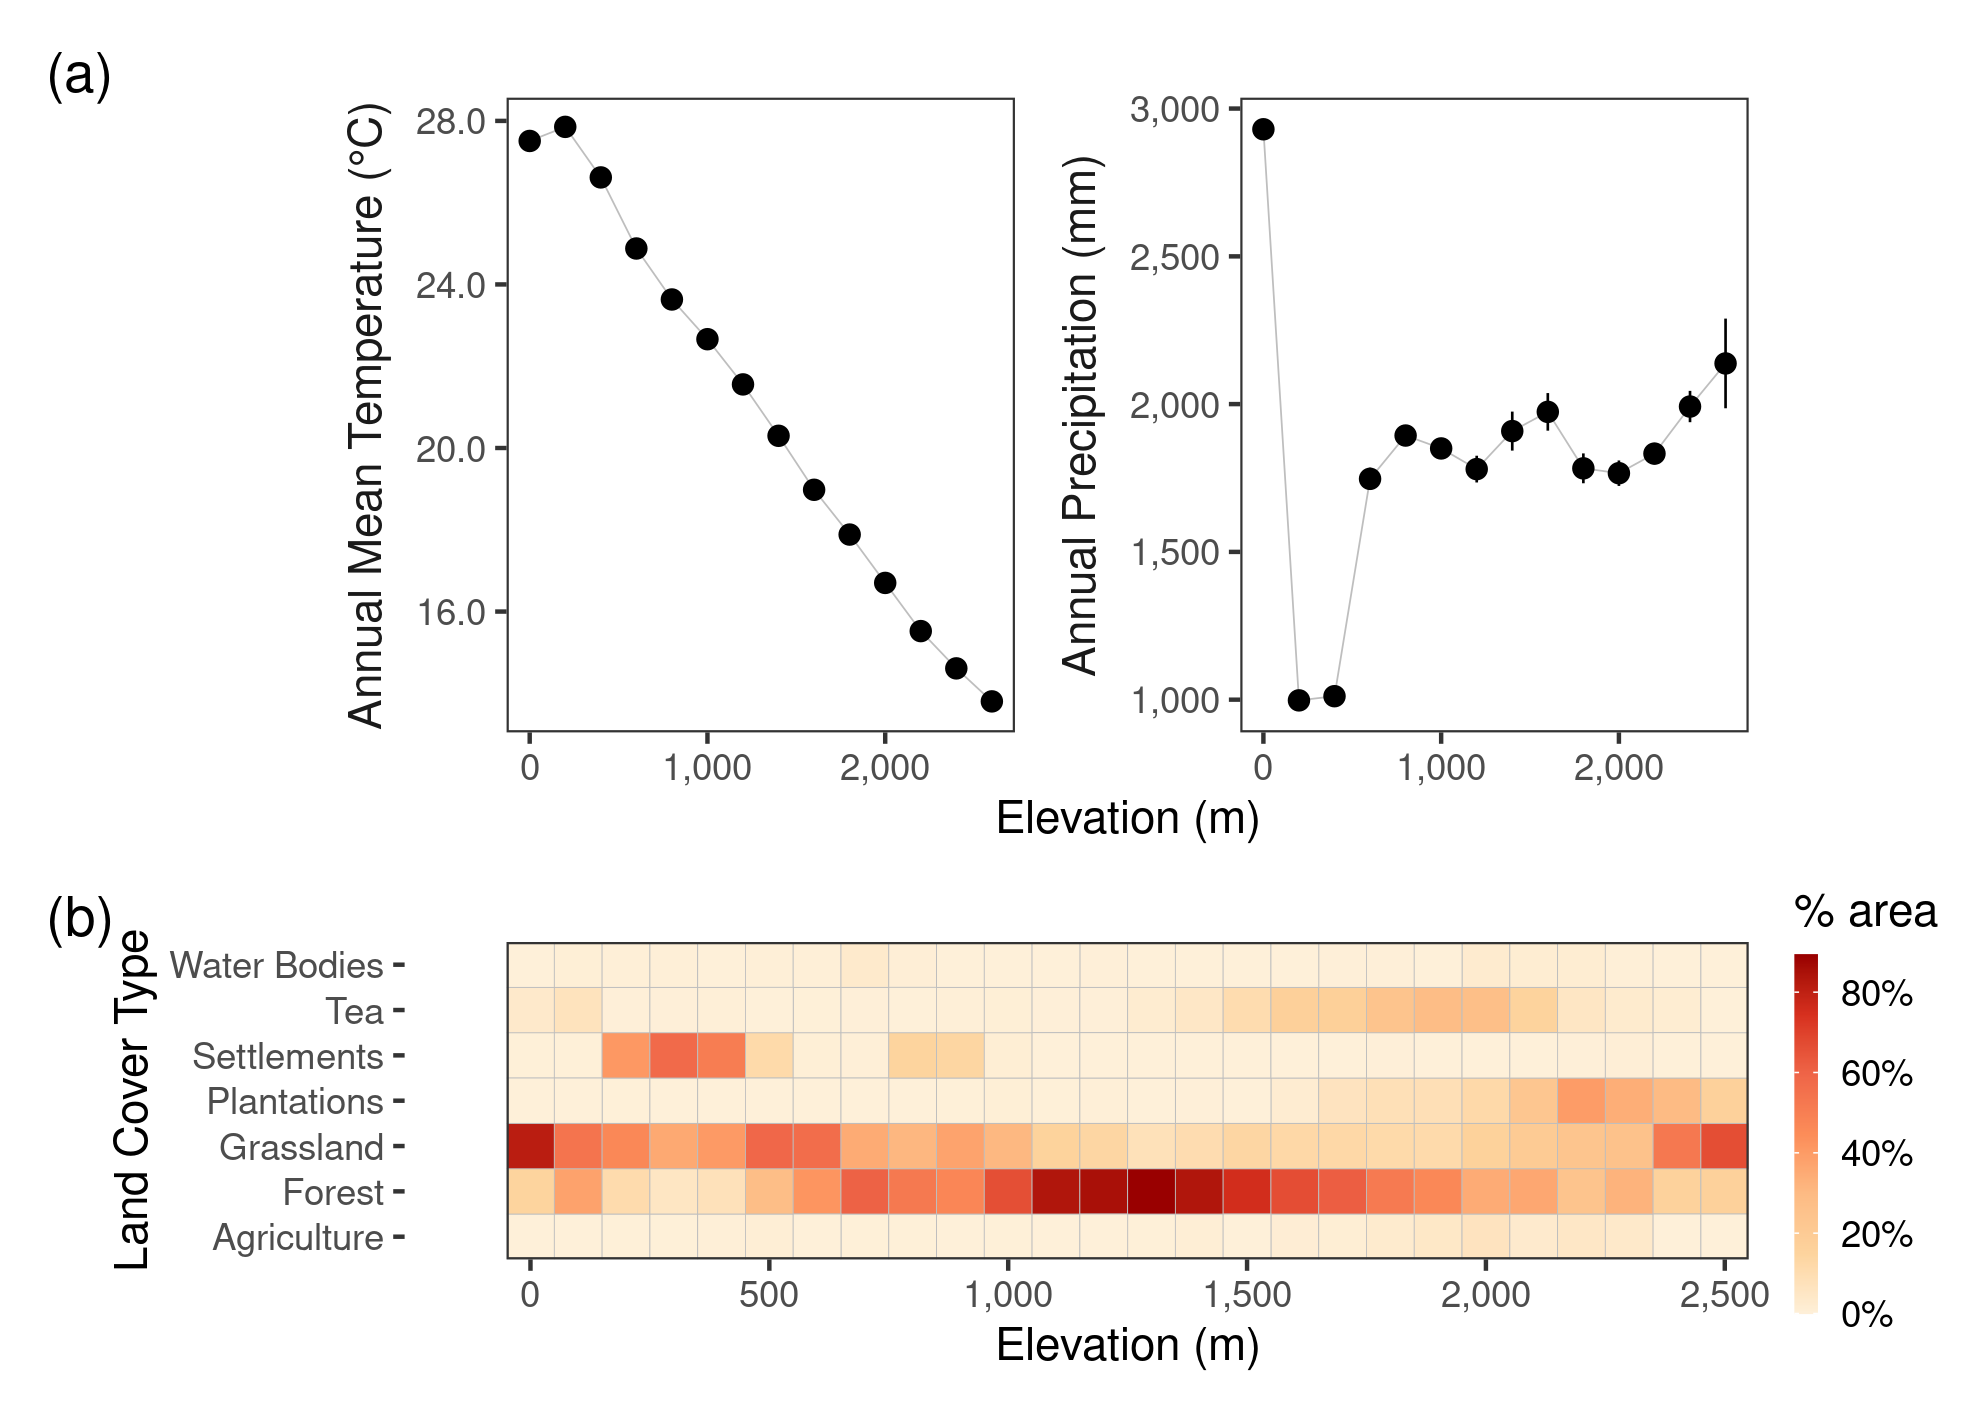
\includegraphics{figs/fig_02.png}
\caption{\textbf{Climate and land cover vary strongly along the elevation gradient in the Nilgiri and Anamalai Hills.}
Both (a) temperature seasonality and (b) precipitation seasonality, between the months of December and May, declines with increasing elevation across the Nilgiri and Anamalai Hills. Climatic variation is not very strongly associated with land cover type, as both natural habitats such as forests, and human-associated habitat types such as plantations show low seasonality in (c) temperature, and (d) precipitation. (e) Most elevations host a range of land cover types: while human-associated habitats such as agriculture are concentrated at lower elevations, and more natural types such as grasslands and forests are associated with higher elevations, each of these types is also found outside their characteristic elevational bands. We calculated climate seasonalities (BIOCLIM 4a and 15: temperature and precipitation, respectively) using CHELSA data over 1979 -- 2013, from December to May (Karger et al.~2017), and present mean seasonality values (vertical bars show standard deviation) for every 200 m elevational band. Land cover types were taken from a reclassification of Roy et al.~(2015; see main text) at 100 m elevational bands. Land cover types covering \textless{} 1\% of an elevational band are shaded grey. All landscape layers were first resampled to 1 km resolution.}
\end{figure}

\hypertarget{preparing-checklist-calibration-index}{%
\section{Preparing Checklist Calibration Index}\label{preparing-checklist-calibration-index}}

Differences in local avifaunal expertise among citizen scientists can lead to biased species detection when compared with data collected by a consistent set of trained observers (van Strien, van Swaay, and Termaat \protect\hyperlink{ref-vanstrien2013}{2013}). Including observer expertise as a detection covariate in occupancy models using eBird data can help account for this variation (Johnston et al. \protect\hyperlink{ref-johnston2018}{2018}). Observer-specific expertise in local avifauna was calculated following (Kelling et al. \protect\hyperlink{ref-kelling2015a}{2015}) as the normalized predicted number of species reported by an observer after 60 minutes of sampling across the most common land cover type within the study area. This score was calculated by examining checklists from anonymized observers across the study area. We modified Kelling et al.~(2015) formulation by including only observations of the 79 species of interest in our calculations. An observer with a higher number of species of interest reported within 60 minutes would have a higher observer-specific expertise score, with respect to the study area.

\hypertarget{prepare-libraries-2}{%
\subsection{Prepare libraries}\label{prepare-libraries-2}}

\begin{Shaded}
\begin{Highlighting}[]

\CommentTok{# load libs}
\KeywordTok{library}\NormalTok{(data.table)}
\KeywordTok{library}\NormalTok{(readxl)}
\KeywordTok{library}\NormalTok{(magrittr)}
\KeywordTok{library}\NormalTok{(stringr)}
\KeywordTok{library}\NormalTok{(dplyr)}
\KeywordTok{library}\NormalTok{(tidyr)}
\KeywordTok{library}\NormalTok{(auk)}

\CommentTok{# get decimal time function}
\KeywordTok{library}\NormalTok{(lubridate)}
\NormalTok{time_to_decimal <-}\StringTok{ }\ControlFlowTok{function}\NormalTok{(x) \{}
\NormalTok{  x <-}\StringTok{ }\NormalTok{lubridate}\OperatorTok{::}\KeywordTok{hms}\NormalTok{(x, }\DataTypeTok{quiet =} \OtherTok{TRUE}\NormalTok{)}
\NormalTok{  lubridate}\OperatorTok{::}\KeywordTok{hour}\NormalTok{(x) }\OperatorTok{+}\StringTok{ }\NormalTok{lubridate}\OperatorTok{::}\KeywordTok{minute}\NormalTok{(x) }\OperatorTok{/}\StringTok{ }\DecValTok{60} \OperatorTok{+}\StringTok{ }\NormalTok{lubridate}\OperatorTok{::}\KeywordTok{second}\NormalTok{(x) }\OperatorTok{/}\StringTok{ }\DecValTok{3600}
\NormalTok{\}}
\end{Highlighting}
\end{Shaded}

\hypertarget{prepare-data}{%
\subsection{Prepare data}\label{prepare-data}}

Here, we go through the data preparation process again because we might want to assess observer expertise over a larger area than the study site.

\begin{Shaded}
\begin{Highlighting}[]
\CommentTok{# Read in shapefile of study area to subset by bounding box}
\KeywordTok{library}\NormalTok{(sf)}
\NormalTok{wg <-}\StringTok{ }\KeywordTok{st_read}\NormalTok{(}\StringTok{"data/spatial/hillsShapefile/Nil_Ana_Pal.shp"}\NormalTok{) }\OperatorTok
\StringTok{  }\KeywordTok{st_transform}\NormalTok{(}\DecValTok{32643}\NormalTok{)}

\CommentTok{# set file paths for auk functions}
\NormalTok{f_in_ebd <-}\StringTok{ }\KeywordTok{file.path}\NormalTok{(}\StringTok{"data/01_ebird-filtered-EBD-westernGhats.txt"}\NormalTok{)}
\NormalTok{f_in_sampling <-}\StringTok{ }\KeywordTok{file.path}\NormalTok{(}\StringTok{"data/01_ebird-filtered-sampling-westernGhats.txt"}\NormalTok{)}

\CommentTok{# run filters using auk packages}
\NormalTok{ebd_filters <-}\StringTok{ }\KeywordTok{auk_ebd}\NormalTok{(f_in_ebd, f_in_sampling) }\OperatorTok
\StringTok{  }\KeywordTok{auk_country}\NormalTok{(}\DataTypeTok{country =} \StringTok{"IN"}\NormalTok{) }\OperatorTok
\StringTok{  }\KeywordTok{auk_state}\NormalTok{(}\KeywordTok{c}\NormalTok{(}\StringTok{"IN-KL"}\NormalTok{, }\StringTok{"IN-TN"}\NormalTok{, }\StringTok{"IN-KA"}\NormalTok{)) }\OperatorTok
\StringTok{  }\CommentTok{# Restricting geography to TamilNadu, Kerala & Karnataka}
\StringTok{  }\KeywordTok{auk_date}\NormalTok{(}\KeywordTok{c}\NormalTok{(}\StringTok{"2013-01-01"}\NormalTok{, }\StringTok{"2021-05-31"}\NormalTok{)) }\OperatorTok
\StringTok{  }\KeywordTok{auk_complete}\NormalTok{()}

\CommentTok{# check filters}
\NormalTok{ebd_filters}

\CommentTok{# specify output location and perform filter}
\NormalTok{f_out_ebd <-}\StringTok{ "data/ebird_for_expertise.txt"}
\NormalTok{f_out_sampling <-}\StringTok{ "data/ebird_sampling_for_expertise.txt"}

\NormalTok{ebd_filtered <-}\StringTok{ }\KeywordTok{auk_filter}\NormalTok{(ebd_filters,}
  \DataTypeTok{file =}\NormalTok{ f_out_ebd,}
  \DataTypeTok{file_sampling =}\NormalTok{ f_out_sampling, }\DataTypeTok{overwrite =} \OtherTok{TRUE}
\NormalTok{)}
\end{Highlighting}
\end{Shaded}

Load in the filtered data and columns of interest.

\begin{Shaded}
\begin{Highlighting}[]
\CommentTok{## Process filtered data}
\CommentTok{# read in the data}
\NormalTok{ebd <-}\StringTok{ }\KeywordTok{fread}\NormalTok{(f_out_ebd)}
\NormalTok{names <-}\StringTok{ }\KeywordTok{names}\NormalTok{(ebd) }\OperatorTok
\StringTok{  }\NormalTok{stringr}\OperatorTok{::}\KeywordTok{str_to_lower}\NormalTok{() }\OperatorTok
\StringTok{  }\NormalTok{stringr}\OperatorTok{::}\KeywordTok{str_replace_all}\NormalTok{(}\StringTok{" "}\NormalTok{, }\StringTok{"_"}\NormalTok{)}

\KeywordTok{setnames}\NormalTok{(ebd, names)}
\CommentTok{# choose columns of interest}
\NormalTok{columnsOfInterest <-}\StringTok{ }\KeywordTok{c}\NormalTok{(}
  \StringTok{"global_unique_identifier"}\NormalTok{, }\StringTok{"scientific_name"}\NormalTok{, }\StringTok{"observation_count"}\NormalTok{,}
  \StringTok{"locality"}\NormalTok{, }\StringTok{"locality_id"}\NormalTok{, }\StringTok{"locality_type"}\NormalTok{, }\StringTok{"latitude"}\NormalTok{,}
  \StringTok{"longitude"}\NormalTok{, }\StringTok{"observation_date"}\NormalTok{,}
  \StringTok{"time_observations_started"}\NormalTok{, }\StringTok{"observer_id"}\NormalTok{,}
  \StringTok{"sampling_event_identifier"}\NormalTok{, }\StringTok{"protocol_type"}\NormalTok{,}
  \StringTok{"duration_minutes"}\NormalTok{, }\StringTok{"effort_distance_km"}\NormalTok{, }\StringTok{"effort_area_ha"}\NormalTok{,}
  \StringTok{"number_observers"}\NormalTok{, }\StringTok{"all_species_reported"}\NormalTok{, }\StringTok{"reviewed"}
\NormalTok{)}

\NormalTok{ebd <-}\StringTok{ }\KeywordTok{setDF}\NormalTok{(ebd) }\OperatorTok
\StringTok{  }\KeywordTok{as_tibble}\NormalTok{() }\OperatorTok
\StringTok{  }\NormalTok{dplyr}\OperatorTok{::}\KeywordTok{select}\NormalTok{(}\KeywordTok{one_of}\NormalTok{(columnsOfInterest))}

\KeywordTok{setDT}\NormalTok{(ebd)}

\CommentTok{# remove checklists or seis with more than 10 obervers}
\NormalTok{ebd <-}\StringTok{ }\KeywordTok{filter}\NormalTok{(ebd, number_observers }\OperatorTok{<=}\StringTok{ }\DecValTok{10}\NormalTok{)}

\CommentTok{# keep only checklists between 5AM and 7PM}
\NormalTok{ebd <-}\StringTok{ }\KeywordTok{filter}\NormalTok{(ebd, time_observations_started }\OperatorTok{>=}\StringTok{ "05:00:00"} \OperatorTok{&}\StringTok{ }\NormalTok{time_observations_started }\OperatorTok{<=}\StringTok{ "19:00:00"}\NormalTok{)}

\CommentTok{# keep only checklists between December 1st and May 31st}
\NormalTok{ebd <-}\StringTok{ }\KeywordTok{filter}\NormalTok{(ebd, }\KeywordTok{month}\NormalTok{(observation_date) }\OperatorTok\StringTok{ }\KeywordTok{c}\NormalTok{(}\DecValTok{1}\NormalTok{, }\DecValTok{2}\NormalTok{, }\DecValTok{3}\NormalTok{, }\DecValTok{4}\NormalTok{, }\DecValTok{5}\NormalTok{, }\DecValTok{12}\NormalTok{))}
\end{Highlighting}
\end{Shaded}

\hypertarget{spatially-explicit-filter-on-checklists}{%
\subsection{Spatially explicit filter on checklists}\label{spatially-explicit-filter-on-checklists}}

\begin{Shaded}
\begin{Highlighting}[]
\CommentTok{# get checklist locations}
\NormalTok{ebd_locs <-}\StringTok{ }\NormalTok{ebd[, .(longitude, latitude)]}
\NormalTok{ebd_locs <-}\StringTok{ }\KeywordTok{setDF}\NormalTok{(ebd_locs) }\OperatorTok\StringTok{ }\KeywordTok{distinct}\NormalTok{()}
\NormalTok{ebd_locs <-}\StringTok{ }\KeywordTok{st_as_sf}\NormalTok{(ebd_locs,}
  \DataTypeTok{coords =} \KeywordTok{c}\NormalTok{(}\StringTok{"longitude"}\NormalTok{, }\StringTok{"latitude"}\NormalTok{)}
\NormalTok{) }\OperatorTok
\StringTok{  `}\DataTypeTok{st_crs<-}\StringTok{`}\NormalTok{(}\DecValTok{4326}\NormalTok{) }\OperatorTok
\StringTok{  }\KeywordTok{bind_cols}\NormalTok{(}\KeywordTok{as_tibble}\NormalTok{(}\KeywordTok{st_coordinates}\NormalTok{(.))) }\OperatorTok
\StringTok{  }\KeywordTok{st_transform}\NormalTok{(}\DecValTok{32643}\NormalTok{) }\OperatorTok
\StringTok{  }\KeywordTok{mutate}\NormalTok{(}\DataTypeTok{id =} \DecValTok{1}\OperatorTok{:}\KeywordTok{nrow}\NormalTok{(.))}

\CommentTok{# check whether to include}
\NormalTok{to_keep <-}\StringTok{ }\KeywordTok{unlist}\NormalTok{(}\KeywordTok{st_contains}\NormalTok{(wg, ebd_locs))}

\CommentTok{# filter locs}
\NormalTok{ebd_locs <-}\StringTok{ }\KeywordTok{filter}\NormalTok{(ebd_locs, id }\OperatorTok\StringTok{ }\NormalTok{to_keep) }\OperatorTok
\StringTok{  }\KeywordTok{bind_cols}\NormalTok{(}\KeywordTok{as_tibble}\NormalTok{(}\KeywordTok{st_coordinates}\NormalTok{(}\KeywordTok{st_as_sf}\NormalTok{(.)))) }\OperatorTok
\StringTok{  }\KeywordTok{st_drop_geometry}\NormalTok{()}
\KeywordTok{names}\NormalTok{(ebd_locs) <-}\StringTok{ }\KeywordTok{c}\NormalTok{(}\StringTok{"longitudeWGS"}\NormalTok{, }\StringTok{"latitudeWGS"}\NormalTok{, }\StringTok{"id"}\NormalTok{, }\StringTok{"longitudeUTM"}\NormalTok{, }\StringTok{"latitudeUTM"}\NormalTok{)}
\end{Highlighting}
\end{Shaded}

\begin{Shaded}
\begin{Highlighting}[]
\NormalTok{ebd <-}\StringTok{ }\NormalTok{ebd[longitude }\OperatorTok\StringTok{ }\NormalTok{ebd_locs}\OperatorTok{$}\NormalTok{longitudeWGS }\OperatorTok{&}\StringTok{ }\NormalTok{latitude }\OperatorTok\StringTok{ }\NormalTok{ebd_locs}\OperatorTok{$}\NormalTok{latitudeWGS, ]}
\end{Highlighting}
\end{Shaded}

\hypertarget{prepare-species-of-interest}{%
\subsection{Prepare species of interest}\label{prepare-species-of-interest}}

\begin{Shaded}
\begin{Highlighting}[]
\CommentTok{# read in species list}
\NormalTok{specieslist <-}\StringTok{ }\KeywordTok{read.csv}\NormalTok{(}\StringTok{"data/species_list.csv"}\NormalTok{)}

\CommentTok{# set species of interest}
\NormalTok{soi <-}\StringTok{ }\NormalTok{specieslist}\OperatorTok{$}\NormalTok{scientific_name}

\NormalTok{ebdSpSum <-}\StringTok{ }\NormalTok{ebd[, .(}
  \DataTypeTok{nSp =}\NormalTok{ .N,}
  \DataTypeTok{totSoiSeen =} \KeywordTok{length}\NormalTok{(}\KeywordTok{intersect}\NormalTok{(scientific_name, soi))}
\NormalTok{),}
\NormalTok{by =}\StringTok{ }\KeywordTok{list}\NormalTok{(sampling_event_identifier)}
\NormalTok{]}

\CommentTok{# write to file and link with checklist id later}
\KeywordTok{fwrite}\NormalTok{(ebdSpSum, }\DataTypeTok{file =} \StringTok{"data/03_data-nspp-per-chk.csv"}\NormalTok{)}
\end{Highlighting}
\end{Shaded}

\hypertarget{prepare-checklists-for-observer-score}{%
\subsection{Prepare checklists for observer score}\label{prepare-checklists-for-observer-score}}

\begin{Shaded}
\begin{Highlighting}[]
\CommentTok{# 1. add new columns of decimal time and julian date}
\NormalTok{ebd[, }\StringTok{`}\DataTypeTok{:=}\StringTok{`}\NormalTok{(}
  \DataTypeTok{decimalTime =} \KeywordTok{time_to_decimal}\NormalTok{(time_observations_started),}
  \DataTypeTok{julianDate =} \KeywordTok{yday}\NormalTok{(}\KeywordTok{as.POSIXct}\NormalTok{(observation_date))}
\NormalTok{)]}

\NormalTok{ebdEffChk <-}\StringTok{ }\KeywordTok{setDF}\NormalTok{(ebd) }\OperatorTok
\StringTok{  }\KeywordTok{mutate}\NormalTok{(}\DataTypeTok{year =} \KeywordTok{year}\NormalTok{(observation_date)) }\OperatorTok
\StringTok{  }\KeywordTok{distinct}\NormalTok{(}
\NormalTok{    sampling_event_identifier, observer_id,}
\NormalTok{    year,}
\NormalTok{    duration_minutes, effort_distance_km, effort_area_ha,}
\NormalTok{    longitude, latitude,}
\NormalTok{    locality, locality_id,}
\NormalTok{    decimalTime, julianDate, number_observers}
\NormalTok{  ) }\OperatorTok
\StringTok{  }\CommentTok{# drop rows with NAs in cols used in the model}
\StringTok{  }\NormalTok{tidyr}\OperatorTok{::}\KeywordTok{drop_na}\NormalTok{(}
\NormalTok{    sampling_event_identifier, observer_id,}
\NormalTok{    duration_minutes, decimalTime, julianDate}
\NormalTok{  ) }\OperatorTok
\StringTok{  }\CommentTok{# drop years below 2013}
\StringTok{  }\KeywordTok{filter}\NormalTok{(year }\OperatorTok{>=}\StringTok{ }\DecValTok{2013}\NormalTok{)}

\CommentTok{# 3. join to covariates and remove large groups (> 10)}
\NormalTok{ebdChkSummary <-}\StringTok{ }\KeywordTok{inner_join}\NormalTok{(ebdEffChk, ebdSpSum)}

\CommentTok{# remove ebird data}
\KeywordTok{rm}\NormalTok{(ebd)}
\KeywordTok{gc}\NormalTok{()}
\end{Highlighting}
\end{Shaded}

\hypertarget{get-landcover}{%
\subsection{Get landcover}\label{get-landcover}}

Read in land cover type data resampled at 1km resolution.

\begin{Shaded}
\begin{Highlighting}[]
\CommentTok{# read in 1km landcover and set 0 to NA}
\KeywordTok{library}\NormalTok{(raster)}
\NormalTok{landcover <-}\StringTok{ }\NormalTok{raster}\OperatorTok{::}\KeywordTok{raster}\NormalTok{(}\StringTok{"data/landUseClassification/lc_01000m.tif"}\NormalTok{)}
\NormalTok{landcover[landcover }\OperatorTok{==}\StringTok{ }\DecValTok{0}\NormalTok{] <-}\StringTok{ }\OtherTok{NA}

\CommentTok{# get locs in utm coords}
\NormalTok{locs <-}\StringTok{ }\KeywordTok{distinct}\NormalTok{(}
\NormalTok{  ebdChkSummary, sampling_event_identifier, longitude, latitude,}
\NormalTok{  locality, locality_id}
\NormalTok{)}
\NormalTok{locs <-}\StringTok{ }\KeywordTok{st_as_sf}\NormalTok{(locs, }\DataTypeTok{coords =} \KeywordTok{c}\NormalTok{(}\StringTok{"longitude"}\NormalTok{, }\StringTok{"latitude"}\NormalTok{)) }\OperatorTok
\StringTok{  `}\DataTypeTok{st_crs<-}\StringTok{`}\NormalTok{(}\DecValTok{4326}\NormalTok{) }\OperatorTok
\StringTok{  }\KeywordTok{st_transform}\NormalTok{(}\DecValTok{32643}\NormalTok{) }\OperatorTok
\StringTok{  }\KeywordTok{st_coordinates}\NormalTok{()}

\CommentTok{# get for unique points}
\NormalTok{landcoverVec <-}\StringTok{ }\NormalTok{raster}\OperatorTok{::}\KeywordTok{extract}\NormalTok{(}
  \DataTypeTok{x =}\NormalTok{ landcover,}
  \DataTypeTok{y =}\NormalTok{ locs}
\NormalTok{)}

\CommentTok{# assign to df and overwrite}
\KeywordTok{setDT}\NormalTok{(ebdChkSummary)[, landcover }\OperatorTok{:}\ErrorTok{=}\StringTok{ }\NormalTok{landcoverVec]}
\end{Highlighting}
\end{Shaded}

\hypertarget{filter-checklist-data}{%
\subsection{Filter checklist data}\label{filter-checklist-data}}

\begin{Shaded}
\begin{Highlighting}[]
\CommentTok{# change names for easy handling}
\KeywordTok{setnames}\NormalTok{(ebdChkSummary, }\KeywordTok{c}\NormalTok{(}
  \StringTok{"locality"}\NormalTok{,}
  \StringTok{"locality_id"}\NormalTok{, }\StringTok{"latitude"}\NormalTok{, }\StringTok{"longitude"}\NormalTok{, }\StringTok{"observer"}\NormalTok{, }\StringTok{"sei"}\NormalTok{,}
  \StringTok{"duration"}\NormalTok{, }\StringTok{"distance"}\NormalTok{, }\StringTok{"area"}\NormalTok{, }\StringTok{"nObs"}\NormalTok{, }\StringTok{"decimalTime"}\NormalTok{, }\StringTok{"julianDate"}\NormalTok{,}
  \StringTok{"year"}\NormalTok{, }\StringTok{"nSp"}\NormalTok{, }\StringTok{"nSoi"}\NormalTok{, }\StringTok{"landcover"}
\NormalTok{))}

\CommentTok{# count data points per observer}
\NormalTok{obscount <-}\StringTok{ }\KeywordTok{count}\NormalTok{(ebdChkSummary, observer) }\OperatorTok
\StringTok{  }\KeywordTok{filter}\NormalTok{(n }\OperatorTok{>=}\StringTok{ }\DecValTok{3}\NormalTok{)}

\CommentTok{# make factor variables and remove obs not in obscount}
\CommentTok{# also remove 0 durations}
\NormalTok{ebdChkSummary <-}\StringTok{ }\NormalTok{ebdChkSummary }\OperatorTok
\StringTok{  }\KeywordTok{mutate}\NormalTok{(}
    \DataTypeTok{distance =} \KeywordTok{ifelse}\NormalTok{(}\KeywordTok{is.na}\NormalTok{(distance), }\DecValTok{0}\NormalTok{, distance),}
    \DataTypeTok{duration =} \KeywordTok{if_else}\NormalTok{(}\KeywordTok{is.na}\NormalTok{(duration), }\FloatTok{0.0}\NormalTok{, }\KeywordTok{as.double}\NormalTok{(duration))}
\NormalTok{  ) }\OperatorTok
\StringTok{  }\KeywordTok{filter}\NormalTok{(}
\NormalTok{    observer }\OperatorTok\StringTok{ }\NormalTok{obscount}\OperatorTok{$}\NormalTok{observer,}
\NormalTok{    duration }\OperatorTok{>}\StringTok{ }\DecValTok{0}\NormalTok{,}
\NormalTok{    duration }\OperatorTok{<=}\StringTok{ }\DecValTok{300}\NormalTok{,}
\NormalTok{    nSoi }\OperatorTok{>=}\StringTok{ }\DecValTok{0}\NormalTok{,}
\NormalTok{    distance }\OperatorTok{<=}\StringTok{ }\DecValTok{5}\NormalTok{,}
    \OperatorTok{!}\KeywordTok{is.na}\NormalTok{(nSoi)}
\NormalTok{  ) }\OperatorTok
\StringTok{  }\KeywordTok{mutate}\NormalTok{(}
    \DataTypeTok{landcover =} \KeywordTok{as.factor}\NormalTok{(landcover),}
    \DataTypeTok{observer =} \KeywordTok{as.factor}\NormalTok{(observer)}
\NormalTok{  ) }\OperatorTok
\StringTok{  }\KeywordTok{drop_na}\NormalTok{(landcover)}

\CommentTok{# editing julian date to model it in a linear fashion}
\KeywordTok{unique}\NormalTok{(ebdChkSummary}\OperatorTok{$}\NormalTok{julianDate)}

\NormalTok{ebdChkSummary <-}\StringTok{ }\NormalTok{ebdChkSummary }\OperatorTok
\StringTok{  }\KeywordTok{mutate}\NormalTok{(}
    \DataTypeTok{newjulianDate =}
      \KeywordTok{case_when}\NormalTok{(}
\NormalTok{        julianDate }\OperatorTok{>=}\StringTok{ }\DecValTok{334} \OperatorTok{&}\StringTok{ }\NormalTok{julianDate }\OperatorTok{<=}\StringTok{ }\DecValTok{365} \OperatorTok{~}\StringTok{ }\NormalTok{(julianDate }\OperatorTok{-}\StringTok{ }\DecValTok{333}\NormalTok{),}
\NormalTok{        julianDate }\OperatorTok{>=}\StringTok{ }\DecValTok{1} \OperatorTok{&}\StringTok{ }\NormalTok{julianDate }\OperatorTok{<=}\StringTok{ }\DecValTok{152} \OperatorTok{~}\StringTok{ }\NormalTok{(julianDate }\OperatorTok{+}\StringTok{ }\DecValTok{31}\NormalTok{)}
\NormalTok{      )}
\NormalTok{  ) }\OperatorTok
\StringTok{  }\KeywordTok{drop_na}\NormalTok{(newjulianDate)}

\CommentTok{# save to file for later reuse}
\KeywordTok{fwrite}\NormalTok{(ebdChkSummary, }\DataTypeTok{file =} \StringTok{"data/03_data-covars-perChklist.csv"}\NormalTok{)}
\end{Highlighting}
\end{Shaded}

\hypertarget{model-observer-expertise}{%
\subsection{Model observer expertise}\label{model-observer-expertise}}

Our observer expertise model aims to include the random intercept effect of observer identity, with a random slope effect of duration. This models the different rate of species accumulation by different observers, as well as their different starting points.

\begin{Shaded}
\begin{Highlighting}[]
\CommentTok{# uses either a subset or all data}
\KeywordTok{library}\NormalTok{(lmerTest)}

\CommentTok{# here we specify a glmm with random effects for observer}
\CommentTok{# time is considered a fixed log predictor and a random slope}
\NormalTok{modObsExp <-}\StringTok{ }\KeywordTok{glmer}\NormalTok{(nSoi }\OperatorTok{~}\StringTok{ }\NormalTok{duration }\OperatorTok{+}\StringTok{ }\KeywordTok{sqrt}\NormalTok{(duration) }\OperatorTok{+}
\StringTok{  }\NormalTok{landcover }\OperatorTok{+}
\StringTok{  }\KeywordTok{sqrt}\NormalTok{(decimalTime) }\OperatorTok{+}
\StringTok{  }\KeywordTok{I}\NormalTok{((}\KeywordTok{sqrt}\NormalTok{(decimalTime))}\OperatorTok{^}\DecValTok{2}\NormalTok{) }\OperatorTok{+}
\StringTok{  }\KeywordTok{log}\NormalTok{(newjulianDate) }\OperatorTok{+}
\StringTok{  }\KeywordTok{I}\NormalTok{((}\KeywordTok{log}\NormalTok{(newjulianDate)}\OperatorTok{^}\DecValTok{2}\NormalTok{)) }\OperatorTok{+}
\StringTok{  }\NormalTok{(}\DecValTok{1} \OperatorTok{|}\StringTok{ }\NormalTok{observer) }\OperatorTok{+}\StringTok{ }\NormalTok{(}\DecValTok{0} \OperatorTok{+}\StringTok{ }\NormalTok{duration }\OperatorTok{|}\StringTok{ }\NormalTok{observer),}
\DataTypeTok{data =}\NormalTok{ ebdChkSummary, }\DataTypeTok{family =} \StringTok{"poisson"}
\NormalTok{)}
\end{Highlighting}
\end{Shaded}

\begin{Shaded}
\begin{Highlighting}[]
\CommentTok{# make dir if absent}
\ControlFlowTok{if}\NormalTok{ (}\OperatorTok{!}\KeywordTok{dir.exists}\NormalTok{(}\StringTok{"data/modOutput"}\NormalTok{)) \{}
  \KeywordTok{dir.create}\NormalTok{(}\StringTok{"data/modOutput"}\NormalTok{)}
\NormalTok{\}}

\CommentTok{# write model output to text file}
\NormalTok{\{}
  \KeywordTok{writeLines}\NormalTok{(R.utils}\OperatorTok{::}\KeywordTok{captureOutput}\NormalTok{(}\KeywordTok{list}\NormalTok{(}\KeywordTok{Sys.time}\NormalTok{(), }\KeywordTok{summary}\NormalTok{(modObsExp))),}
    \DataTypeTok{con =} \StringTok{"data/modOutput/03_model-output-expertise.txt"}
\NormalTok{  )}
\NormalTok{\}}
\end{Highlighting}
\end{Shaded}

\begin{Shaded}
\begin{Highlighting}[]
\CommentTok{# make df with means}
\NormalTok{observer <-}\StringTok{ }\KeywordTok{unique}\NormalTok{(ebdChkSummary}\OperatorTok{$}\NormalTok{observer)}

\CommentTok{# predict at 60 mins on the most common landcover (deciduous forests)}
\NormalTok{dfPredict <-}\StringTok{ }\NormalTok{ebdChkSummary }\OperatorTok
\StringTok{  }\KeywordTok{summarise_at}\NormalTok{(}\KeywordTok{vars}\NormalTok{(duration, decimalTime, newjulianDate), }\KeywordTok{list}\NormalTok{(}\OperatorTok{~}\StringTok{ }\KeywordTok{mean}\NormalTok{(.))) }\OperatorTok
\StringTok{  }\KeywordTok{mutate}\NormalTok{(}\DataTypeTok{duration =} \DecValTok{60}\NormalTok{, }\DataTypeTok{landcover =} \KeywordTok{as.factor}\NormalTok{(}\DecValTok{2}\NormalTok{)) }\OperatorTok
\StringTok{  }\NormalTok{tidyr}\OperatorTok{::}\KeywordTok{crossing}\NormalTok{(observer)}

\CommentTok{# run predict from model on it}
\NormalTok{dfPredict <-}\StringTok{ }\KeywordTok{mutate}\NormalTok{(dfPredict,}
  \DataTypeTok{score =} \KeywordTok{predict}\NormalTok{(modObsExp,}
    \DataTypeTok{newdata =}\NormalTok{ dfPredict,}
    \DataTypeTok{type =} \StringTok{"response"}\NormalTok{,}
    \DataTypeTok{allow.new.levels =} \OtherTok{TRUE}
\NormalTok{  )}
\NormalTok{) }\OperatorTok
\StringTok{  }\KeywordTok{mutate}\NormalTok{(}\DataTypeTok{score =}\NormalTok{ scales}\OperatorTok{::}\KeywordTok{rescale}\NormalTok{(score))}
\end{Highlighting}
\end{Shaded}

\begin{Shaded}
\begin{Highlighting}[]
\KeywordTok{fwrite}\NormalTok{(dfPredict }\OperatorTok\StringTok{ }\NormalTok{dplyr}\OperatorTok{::}\KeywordTok{select}\NormalTok{(observer, score),}
  \DataTypeTok{file =} \StringTok{"data/03_data-obsExpertise-score.csv"}
\NormalTok{)}
\end{Highlighting}
\end{Shaded}

\hypertarget{examining-spatial-sampling-bias}{%
\section{Examining Spatial Sampling Bias}\label{examining-spatial-sampling-bias}}

The goal of this section is to show how far each checklist location is from the nearest road, and how far each site is from its nearest neighbour. This follows finding the pairwise distance between a large number of unique checklist locations to a vast number of roads, as well as to each other.

\hypertarget{prepare-libraries-3}{%
\subsection{Prepare libraries}\label{prepare-libraries-3}}

\begin{Shaded}
\begin{Highlighting}[]
\CommentTok{# load libraries}
\CommentTok{# for data}
\KeywordTok{library}\NormalTok{(sf)}
\KeywordTok{library}\NormalTok{(rnaturalearth)}
\KeywordTok{library}\NormalTok{(dplyr)}
\KeywordTok{library}\NormalTok{(readr)}
\KeywordTok{library}\NormalTok{(purrr)}

\CommentTok{# for plotting}
\KeywordTok{library}\NormalTok{(scales)}
\KeywordTok{library}\NormalTok{(ggplot2)}
\KeywordTok{library}\NormalTok{(ggspatial)}
\KeywordTok{library}\NormalTok{(colorspace)}

\CommentTok{# round any function}
\NormalTok{round_any <-}\StringTok{ }\ControlFlowTok{function}\NormalTok{(x, }\DataTypeTok{accuracy =} \DecValTok{20000}\NormalTok{) \{}
  \KeywordTok{round}\NormalTok{(x }\OperatorTok{/}\StringTok{ }\NormalTok{accuracy) }\OperatorTok{*}\StringTok{ }\NormalTok{accuracy}
\NormalTok{\}}
\CommentTok{# ci function}
\NormalTok{ci <-}\StringTok{ }\ControlFlowTok{function}\NormalTok{(x) \{}
  \KeywordTok{qnorm}\NormalTok{(}\FloatTok{0.975}\NormalTok{) }\OperatorTok{*}\StringTok{ }\KeywordTok{sd}\NormalTok{(x, }\DataTypeTok{na.rm =} \OtherTok{TRUE}\NormalTok{) }\OperatorTok{/}\StringTok{ }\KeywordTok{sqrt}\NormalTok{(}\KeywordTok{length}\NormalTok{(x))}
\NormalTok{\}}
\end{Highlighting}
\end{Shaded}

\hypertarget{read-checklist-data}{%
\subsection{Read checklist data}\label{read-checklist-data}}

Read in checklist data with distance to nearest neighbouring site, and the distance to the nearest road.

\begin{Shaded}
\begin{Highlighting}[]
\CommentTok{# read from local file}
\NormalTok{chkCovars <-}\StringTok{ }\KeywordTok{read_csv}\NormalTok{(}\StringTok{"data/03_data-covars-perChklist.csv"}\NormalTok{)}
\end{Highlighting}
\end{Shaded}

\hypertarget{spatially-explicit-filter-on-checklists-1}{%
\subsubsection{Spatially explicit filter on checklists}\label{spatially-explicit-filter-on-checklists-1}}

We filter the checklists by the boundary of the study area. This is \emph{not} the extent.

\begin{Shaded}
\begin{Highlighting}[]
\NormalTok{chkCovars <-}\StringTok{ }\KeywordTok{st_as_sf}\NormalTok{(chkCovars, }\DataTypeTok{coords =} \KeywordTok{c}\NormalTok{(}\StringTok{"longitude"}\NormalTok{, }\StringTok{"latitude"}\NormalTok{)) }\OperatorTok
\StringTok{  `}\DataTypeTok{st_crs<-}\StringTok{`}\NormalTok{(}\DecValTok{4326}\NormalTok{) }\OperatorTok
\StringTok{  }\KeywordTok{st_transform}\NormalTok{(}\DecValTok{32643}\NormalTok{)}

\CommentTok{# read wg}
\NormalTok{wg <-}\StringTok{ }\KeywordTok{st_read}\NormalTok{(}\StringTok{"data/spatial/hillsShapefile/Nil_Ana_Pal.shp"}\NormalTok{) }\OperatorTok
\StringTok{  }\KeywordTok{st_transform}\NormalTok{(}\DecValTok{32643}\NormalTok{)}
\CommentTok{# get bounding box}
\NormalTok{bbox <-}\StringTok{ }\KeywordTok{st_bbox}\NormalTok{(wg)}

\CommentTok{# spatial subset}
\NormalTok{chkCovars <-}\StringTok{ }\NormalTok{chkCovars }\OperatorTok
\StringTok{  }\KeywordTok{mutate}\NormalTok{(}\DataTypeTok{id =} \DecValTok{1}\OperatorTok{:}\KeywordTok{nrow}\NormalTok{(.)) }\OperatorTok
\StringTok{  }\KeywordTok{filter}\NormalTok{(id }\OperatorTok\StringTok{ }\KeywordTok{unlist}\NormalTok{(}\KeywordTok{st_contains}\NormalTok{(wg, chkCovars)))}
\end{Highlighting}
\end{Shaded}

\hypertarget{get-background-land-for-plotting}{%
\subsubsection{Get background land for plotting}\label{get-background-land-for-plotting}}

\begin{Shaded}
\begin{Highlighting}[]
\CommentTok{# add land}
\NormalTok{land <-}\StringTok{ }\KeywordTok{ne_countries}\NormalTok{(}
  \DataTypeTok{scale =} \DecValTok{50}\NormalTok{, }\DataTypeTok{type =} \StringTok{"countries"}\NormalTok{, }\DataTypeTok{continent =} \StringTok{"asia"}\NormalTok{,}
  \DataTypeTok{country =} \StringTok{"india"}\NormalTok{,}
  \DataTypeTok{returnclass =} \KeywordTok{c}\NormalTok{(}\StringTok{"sf"}\NormalTok{)}
\NormalTok{) }\OperatorTok
\StringTok{  }\KeywordTok{st_transform}\NormalTok{(}\DecValTok{32643}\NormalTok{)}

\CommentTok{# add roads data}
\NormalTok{roads <-}\StringTok{ }\KeywordTok{st_read}\NormalTok{(}\StringTok{"data/spatial/roads_studysite_2019/roads_studysite_2019.shp"}\NormalTok{) }\OperatorTok
\StringTok{  }\KeywordTok{st_transform}\NormalTok{(}\DecValTok{32643}\NormalTok{)}
\end{Highlighting}
\end{Shaded}

\hypertarget{prepare-main-text-figure-3}{%
\subsection{Prepare Main Text Figure 3}\label{prepare-main-text-figure-3}}

\hypertarget{prepare-histogram-of-distance-to-roads}{%
\subsubsection{Prepare histogram of distance to roads}\label{prepare-histogram-of-distance-to-roads}}

Figure code is hidden in versions rendered as HTML or PDF.

\hypertarget{table-distance-to-roads}{%
\subsubsection{Table: Distance to roads}\label{table-distance-to-roads}}

\begin{Shaded}
\begin{Highlighting}[]
\CommentTok{# write the mean and ci95 to file}
\NormalTok{chkCovars }\OperatorTok
\StringTok{  }\KeywordTok{st_drop_geometry}\NormalTok{() }\OperatorTok
\StringTok{  }\NormalTok{dplyr}\OperatorTok{::}\KeywordTok{select}\NormalTok{(dist_road, nnb) }\OperatorTok
\StringTok{  }\NormalTok{tidyr}\OperatorTok{::}\KeywordTok{pivot_longer}\NormalTok{(}
    \DataTypeTok{cols =} \KeywordTok{c}\NormalTok{(}\StringTok{"dist_road"}\NormalTok{, }\StringTok{"nnb"}\NormalTok{),}
    \DataTypeTok{names_to =} \StringTok{"variable"}
\NormalTok{  ) }\OperatorTok
\StringTok{  }\KeywordTok{group_by}\NormalTok{(variable) }\OperatorTok
\StringTok{  }\KeywordTok{summarise_at}\NormalTok{(}
    \KeywordTok{vars}\NormalTok{(value),}
    \KeywordTok{list}\NormalTok{(}\OperatorTok{~}\StringTok{ }\KeywordTok{mean}\NormalTok{(.), }\OperatorTok{~}\StringTok{ }\KeywordTok{sd}\NormalTok{(.), }\OperatorTok{~}\StringTok{ }\KeywordTok{min}\NormalTok{(.), }\OperatorTok{~}\StringTok{ }\KeywordTok{max}\NormalTok{(.))}
\NormalTok{  ) }\OperatorTok
\StringTok{  }\KeywordTok{write_csv}\NormalTok{(}\StringTok{"data/results/distance_roads_sites.csv"}\NormalTok{)}
\end{Highlighting}
\end{Shaded}

\hypertarget{distance-to-nearest-neighbouring-site}{%
\subsubsection{Distance to nearest neighbouring site}\label{distance-to-nearest-neighbouring-site}}

\begin{Shaded}
\begin{Highlighting}[]
\CommentTok{# get unique locations from checklists}
\NormalTok{locs_unique <-}\StringTok{ }\KeywordTok{cbind}\NormalTok{(}
  \KeywordTok{st_drop_geometry}\NormalTok{(chkCovars),}
  \KeywordTok{st_coordinates}\NormalTok{(chkCovars)}
\NormalTok{) }\OperatorTok
\StringTok{  }\KeywordTok{as_tibble}\NormalTok{()}

\NormalTok{locs_unique <-}\StringTok{ }\KeywordTok{distinct}\NormalTok{(locs_unique, X, Y, }\DataTypeTok{.keep_all =}\NormalTok{ T)}
\end{Highlighting}
\end{Shaded}

Figure code is hidden in versions rendered as HTML and PDF.

\hypertarget{spatial-distribution-of-distances-to-neighbours}{%
\subsubsection{Spatial distribution of distances to neighbours}\label{spatial-distribution-of-distances-to-neighbours}}

Figure code is hidden in HTML and PDF versions, consult the Rmarkdown file.

\begin{figure}
\centering
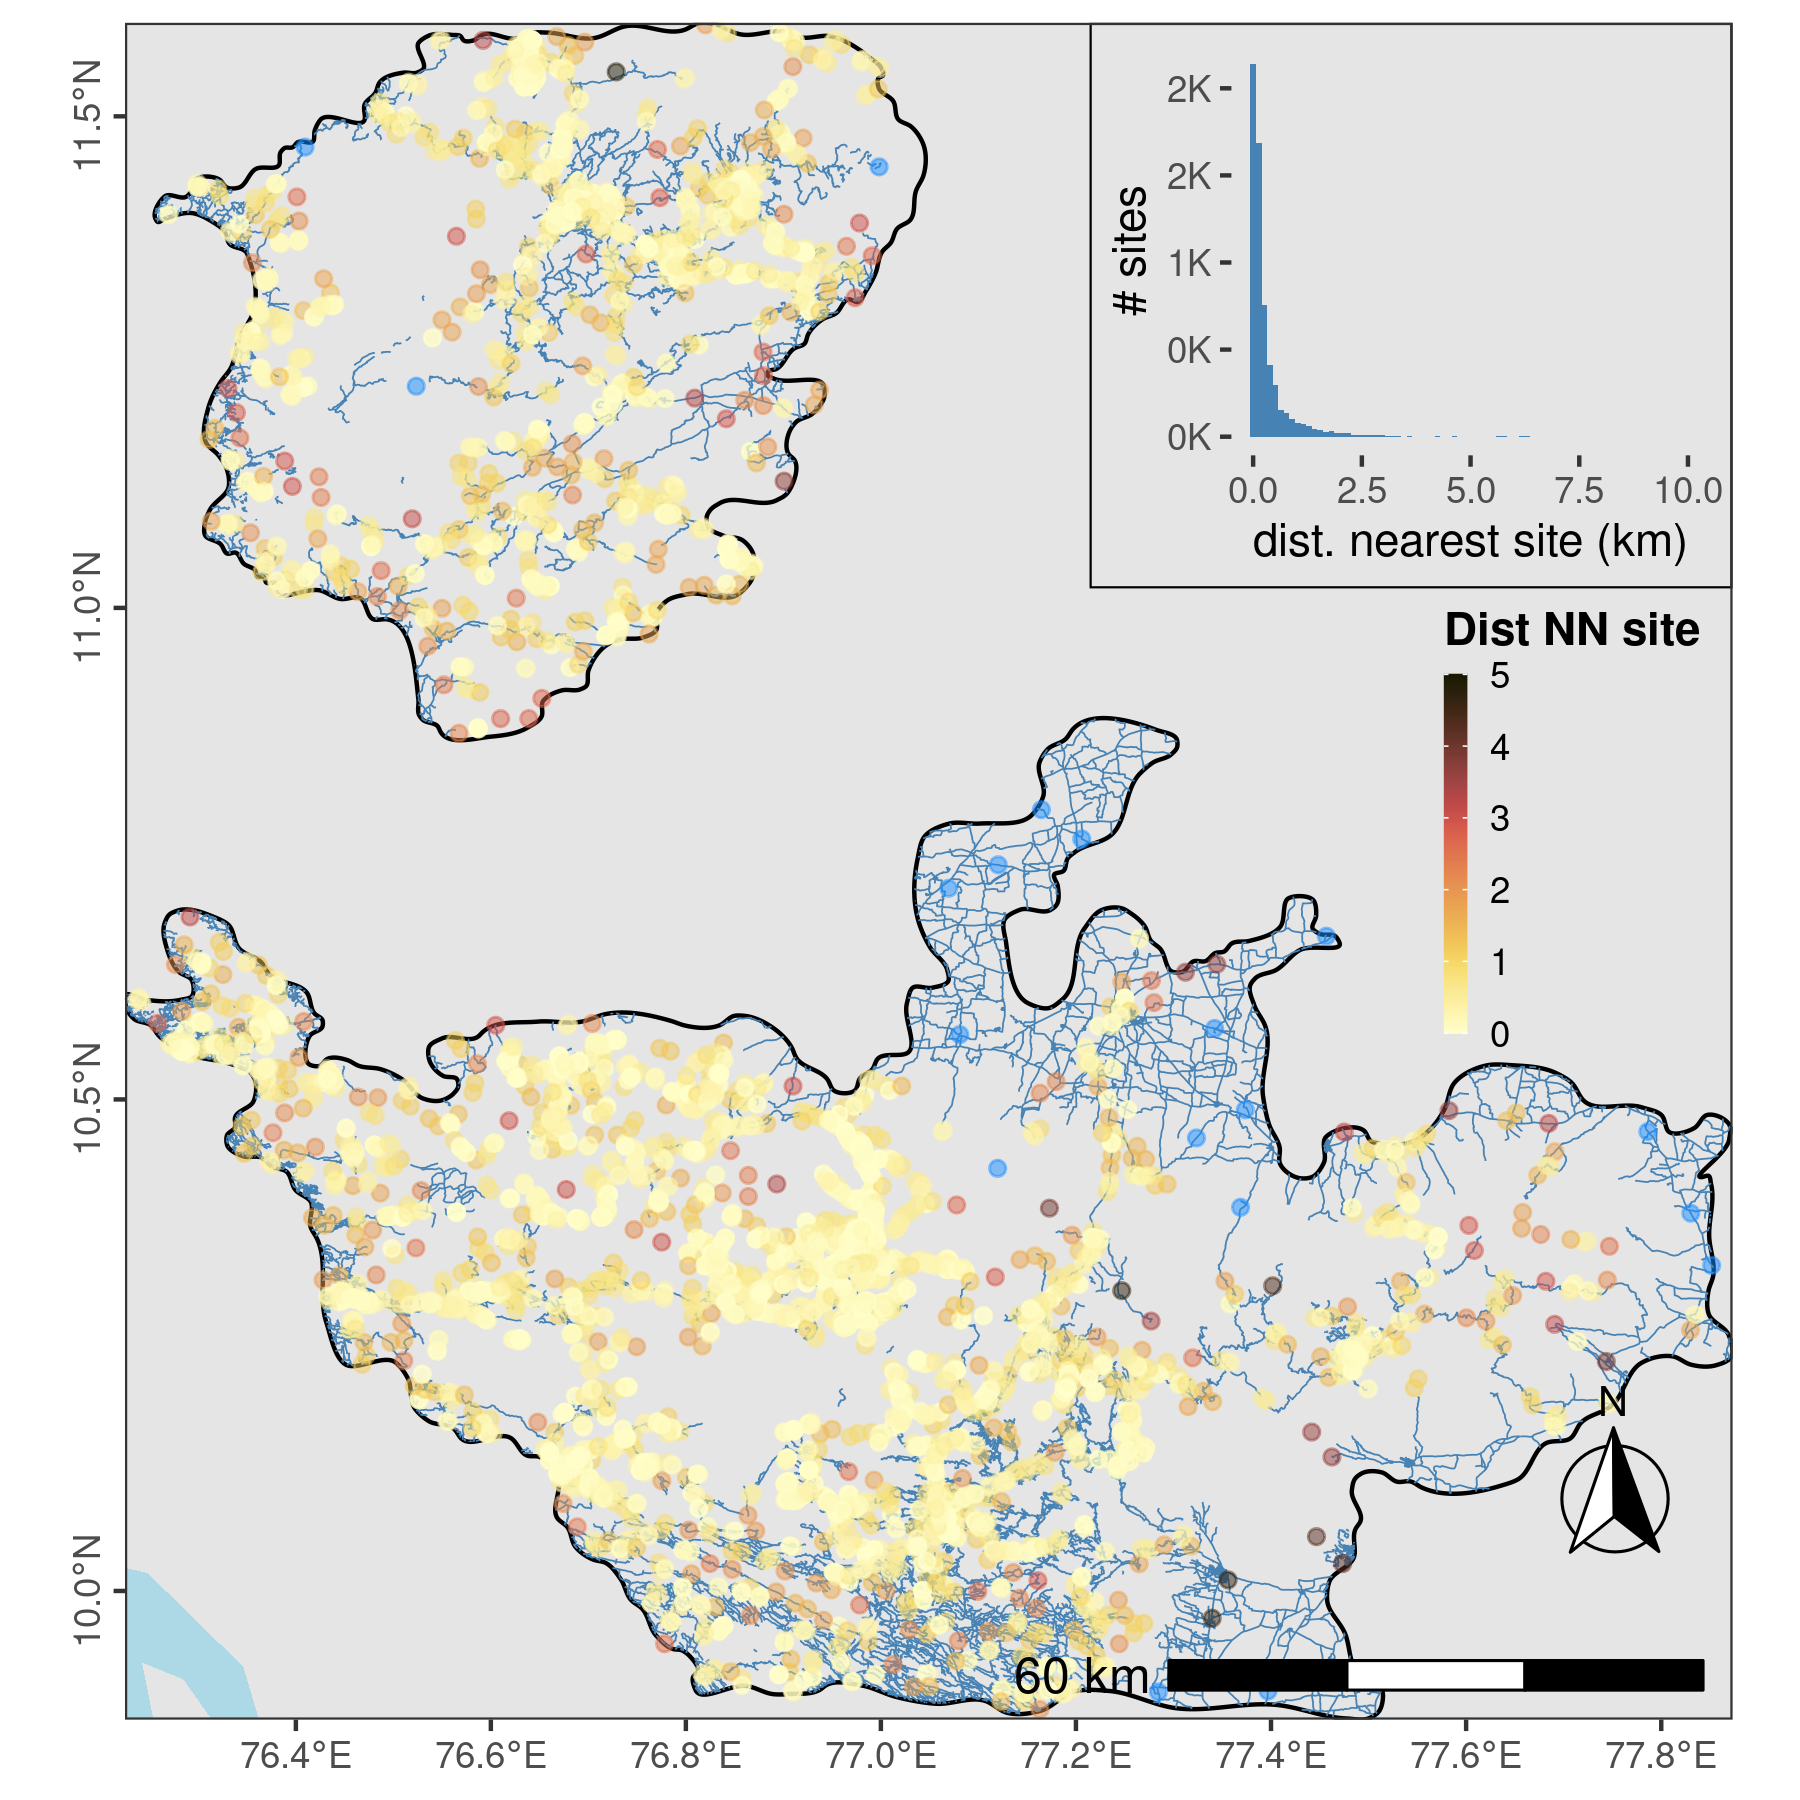
\includegraphics{figs/fig_site_nnb.png}
\caption{Most observation sites are within 300m of another site.}
\end{figure}

\hypertarget{figure-spatial-sampling-bias}{%
\subsection{Figure: Spatial sampling bias}\label{figure-spatial-sampling-bias}}

\begin{Shaded}
\begin{Highlighting}[]
\CommentTok{# get locations}
\NormalTok{points <-}\StringTok{ }\NormalTok{chkCovars }\OperatorTok
\StringTok{  }\KeywordTok{bind_cols}\NormalTok{(}\KeywordTok{as_tibble}\NormalTok{(}\KeywordTok{st_coordinates}\NormalTok{(.))) }\OperatorTok
\StringTok{  }\KeywordTok{st_drop_geometry}\NormalTok{() }\OperatorTok
\StringTok{  }\KeywordTok{mutate}\NormalTok{(}\DataTypeTok{X =} \KeywordTok{round_any}\NormalTok{(X, }\DecValTok{2500}\NormalTok{), }\DataTypeTok{Y =} \KeywordTok{round_any}\NormalTok{(Y, }\DecValTok{2500}\NormalTok{))}

\CommentTok{# count points}
\NormalTok{points <-}\StringTok{ }\KeywordTok{count}\NormalTok{(points, X, Y)}
\end{Highlighting}
\end{Shaded}

Figure code is hidden in versions rendered as HTML and PDF.

\begin{Shaded}
\begin{Highlighting}[]
\CommentTok{# save as png}
\KeywordTok{ggsave}\NormalTok{(}
\NormalTok{  fig_checklists_grid,}
  \DataTypeTok{filename =} \StringTok{"figs/fig_spatial_bias.png"}
\NormalTok{)}

\CommentTok{# save figure as Robject for next plot}
\KeywordTok{save}\NormalTok{(fig_checklists_grid, }\DataTypeTok{file =} \StringTok{"data/fig_checklists_grid.Rds"}\NormalTok{)}
\end{Highlighting}
\end{Shaded}

\begin{figure}
\centering
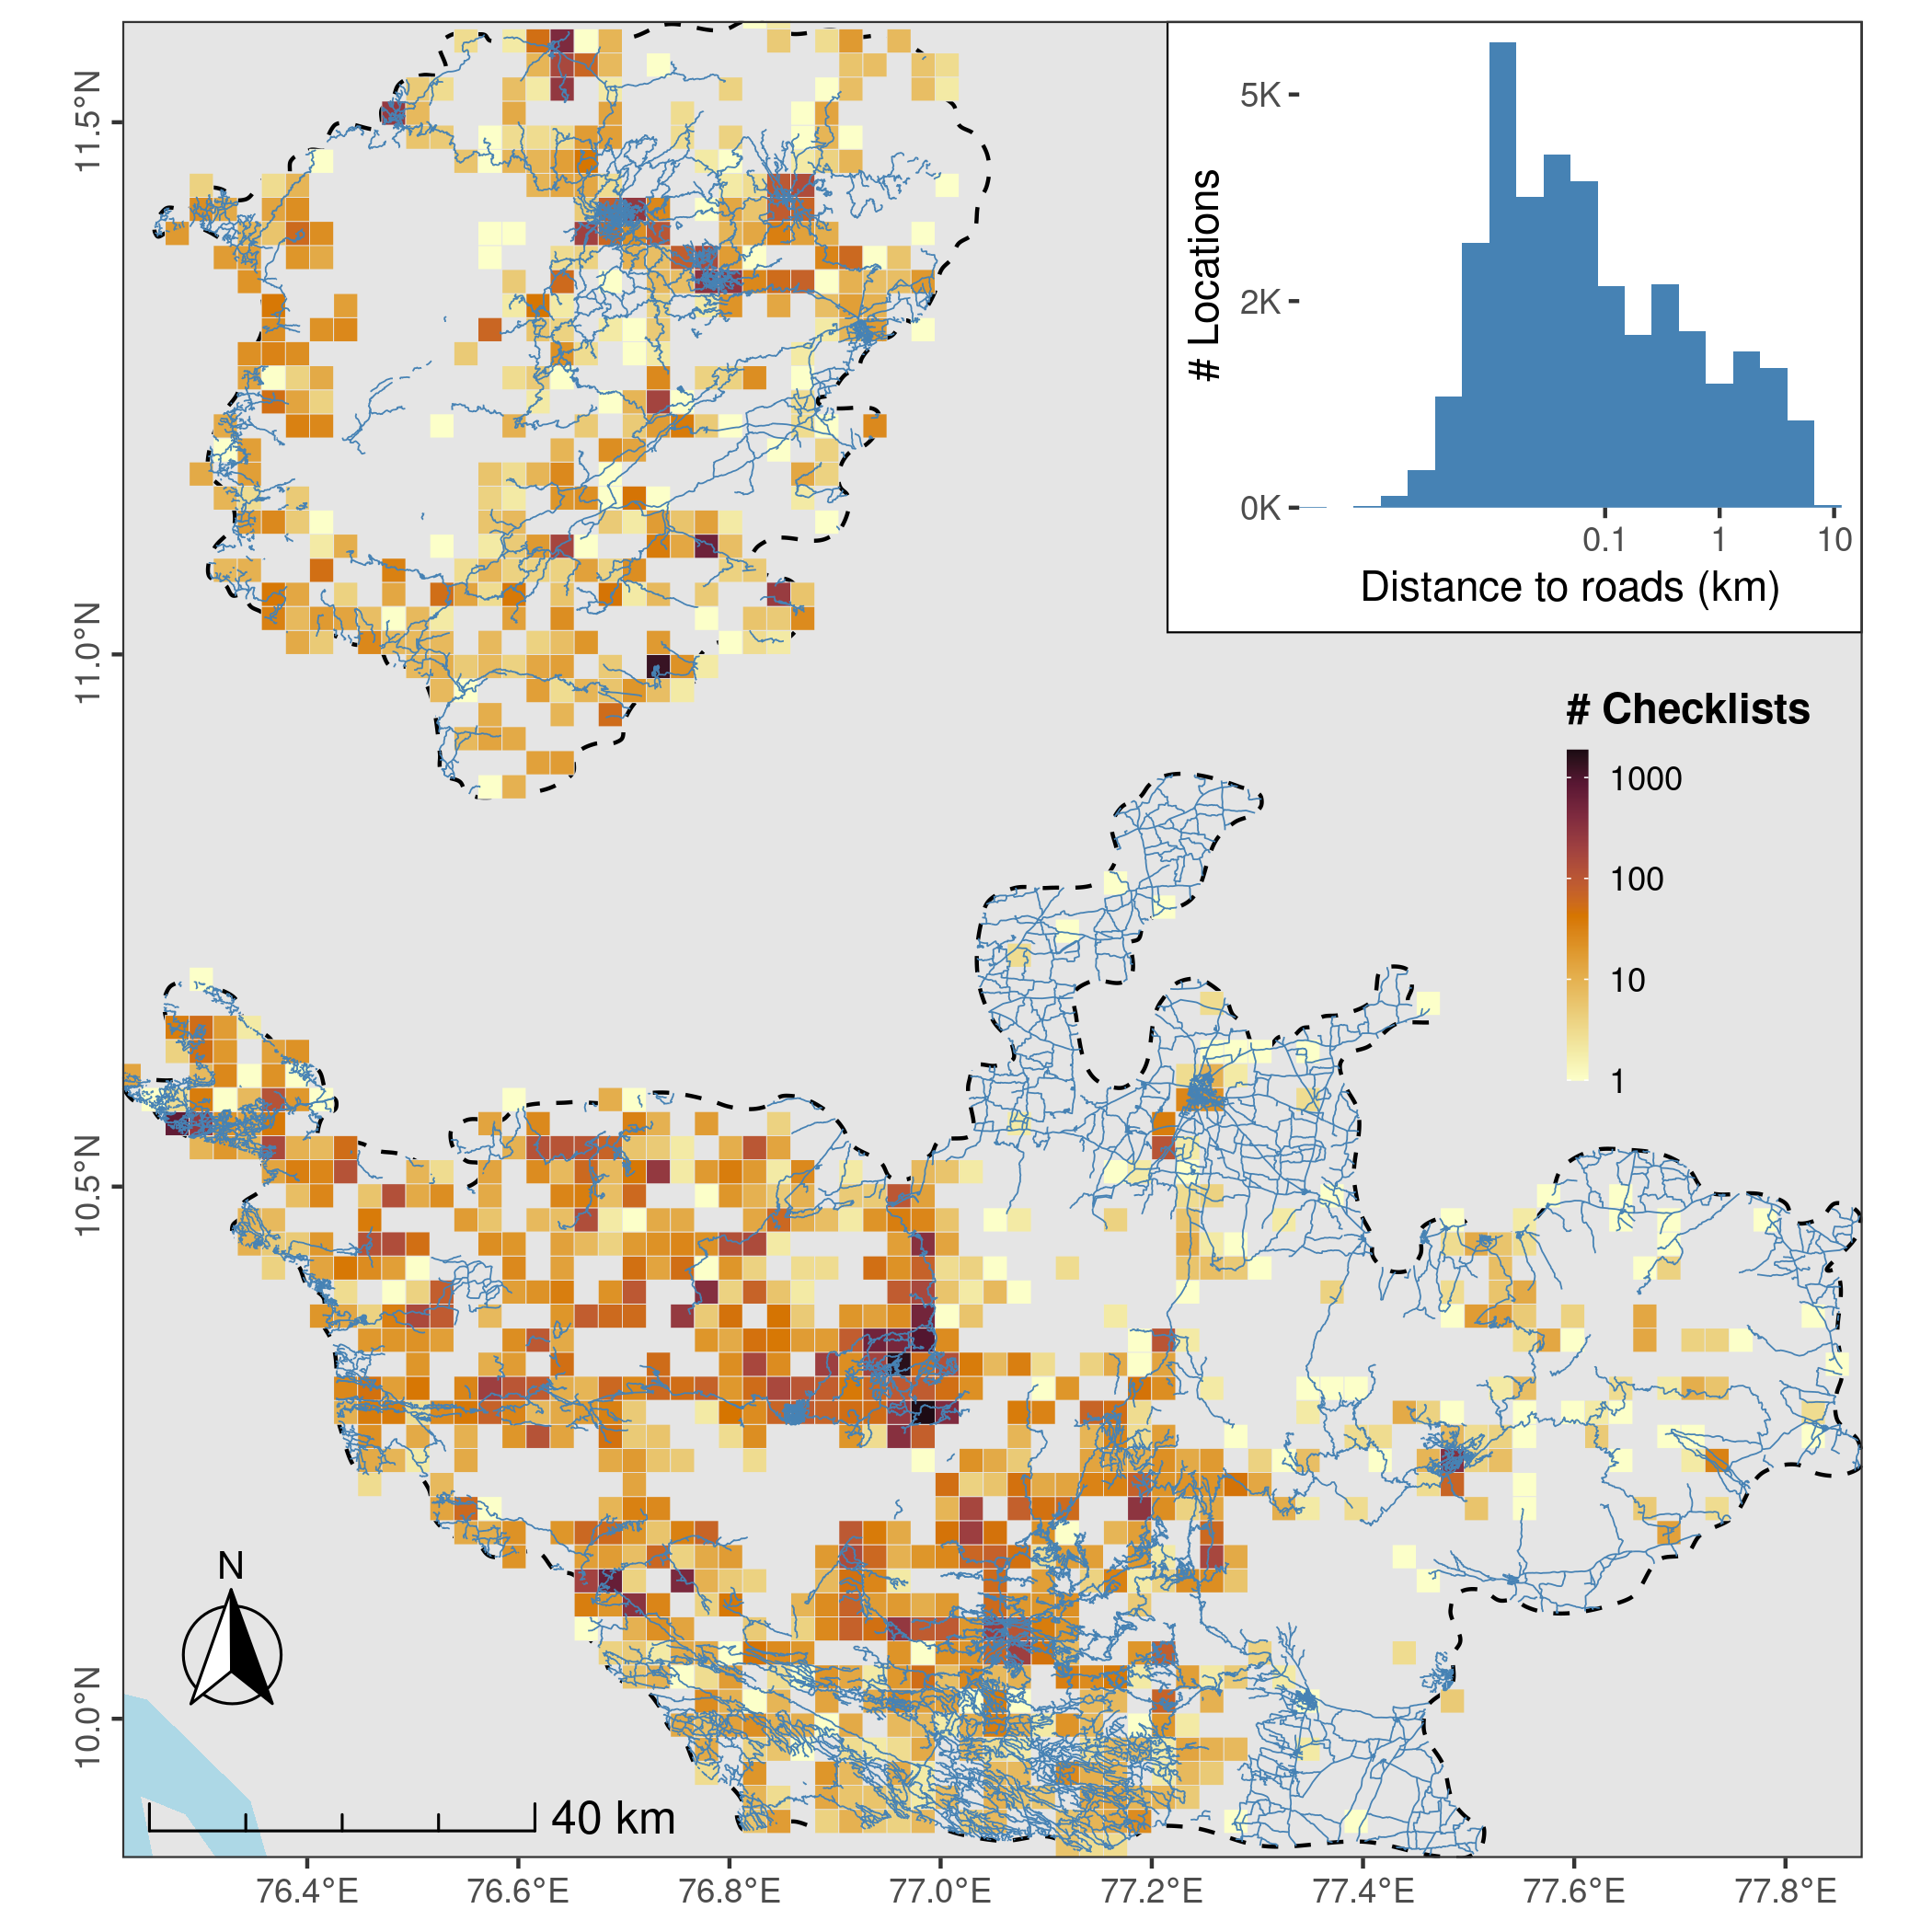
\includegraphics{figs/fig_spatial_bias.png}
\caption{Sampling effort across the Nilgiri and Anamalai Hills, in the form of eBird checklists reported by birdwatchers, mostly takes place along roads, with the majority of checklists located \textless{} 1 km from a roadway (see distribution in inset), and therefore, only about 300m, on average, from the location of another checklist. Each cell here is 2.5km x 2.5km.}
\end{figure}

\hypertarget{checking-temporal-sampling-frequency}{%
\section{Checking Temporal Sampling Frequency}\label{checking-temporal-sampling-frequency}}

How often are checklists recorded in each grid cell?

\hypertarget{load-libraries}{%
\subsection{Load libraries}\label{load-libraries}}

\begin{Shaded}
\begin{Highlighting}[]
\CommentTok{# load libraries}
\KeywordTok{library}\NormalTok{(tidyverse)}
\KeywordTok{library}\NormalTok{(sf)}

\CommentTok{# for plotting}
\KeywordTok{library}\NormalTok{(ggplot2)}
\KeywordTok{library}\NormalTok{(colorspace)}
\KeywordTok{library}\NormalTok{(scico)}
\KeywordTok{library}\NormalTok{(ggthemes)}
\KeywordTok{library}\NormalTok{(ggspatial)}
\KeywordTok{library}\NormalTok{(patchwork)}
\end{Highlighting}
\end{Shaded}

\hypertarget{load-checklist-data}{%
\subsection{Load checklist data}\label{load-checklist-data}}

Here we load filtered checklist data and convert to UTM 43N coordinates.

\begin{Shaded}
\begin{Highlighting}[]
\CommentTok{# load checklist data}
\KeywordTok{load}\NormalTok{(}\StringTok{"data/01_data_prelim_processing.rdata"}\NormalTok{)}

\CommentTok{# get checklists}
\NormalTok{data <-}\StringTok{ }\KeywordTok{distinct}\NormalTok{(}
\NormalTok{  dataGrouped, sampling_event_identifier, observation_date,}
\NormalTok{  longitude, latitude}
\NormalTok{)}

\CommentTok{# remove old data}
\KeywordTok{rm}\NormalTok{(dataGrouped)}

\CommentTok{# transform to UTM 43N}
\NormalTok{data <-}\StringTok{ }\KeywordTok{st_as_sf}\NormalTok{(data, }\DataTypeTok{coords =} \KeywordTok{c}\NormalTok{(}\StringTok{"longitude"}\NormalTok{, }\StringTok{"latitude"}\NormalTok{), }\DataTypeTok{crs =} \DecValTok{4326}\NormalTok{)}
\NormalTok{data <-}\StringTok{ }\KeywordTok{st_transform}\NormalTok{(data, }\DataTypeTok{crs =} \DecValTok{32643}\NormalTok{)}

\CommentTok{# get coordinates and bind to data}
\NormalTok{data <-}\StringTok{ }\KeywordTok{cbind}\NormalTok{(}
  \KeywordTok{st_drop_geometry}\NormalTok{(data),}
  \KeywordTok{st_coordinates}\NormalTok{(data)}
\NormalTok{)}

\CommentTok{# bin to 1000m}
\NormalTok{data <-}\StringTok{ }\KeywordTok{mutate}\NormalTok{(data,}
  \DataTypeTok{X =}\NormalTok{ plyr}\OperatorTok{::}\KeywordTok{round_any}\NormalTok{(X, }\DecValTok{2500}\NormalTok{),}
  \DataTypeTok{Y =}\NormalTok{ plyr}\OperatorTok{::}\KeywordTok{round_any}\NormalTok{(Y, }\DecValTok{2500}\NormalTok{)}
\NormalTok{)}
\end{Highlighting}
\end{Shaded}

\hypertarget{get-time-differences-per-grid-cell}{%
\subsection{Get time differences per grid cell}\label{get-time-differences-per-grid-cell}}

\begin{Shaded}
\begin{Highlighting}[]
\CommentTok{# get time differences in days}
\NormalTok{data <-}\StringTok{ }\KeywordTok{mutate}\NormalTok{(data, }\DataTypeTok{observation_date =} \KeywordTok{as.POSIXct}\NormalTok{(observation_date))}
\NormalTok{data <-}\StringTok{ }\KeywordTok{nest}\NormalTok{(data, }\DataTypeTok{data =} \KeywordTok{c}\NormalTok{(}\StringTok{"sampling_event_identifier"}\NormalTok{, }\StringTok{"observation_date"}\NormalTok{))}

\CommentTok{# map over data}
\NormalTok{data <-}\StringTok{ }\KeywordTok{mutate}\NormalTok{(data,}
  \DataTypeTok{lag_metrics =} \KeywordTok{lapply}\NormalTok{(data, }\ControlFlowTok{function}\NormalTok{(df) \{}
\NormalTok{    df <-}\StringTok{ }\KeywordTok{arrange}\NormalTok{(df, observation_date)}

\NormalTok{    lag <-}\StringTok{ }\KeywordTok{as.numeric}\NormalTok{(}\KeywordTok{diff}\NormalTok{(df}\OperatorTok{$}\NormalTok{observation_date, }\DataTypeTok{na.rm =} \OtherTok{TRUE}\NormalTok{) }\OperatorTok{/}\StringTok{ }\NormalTok{(}\DecValTok{24} \OperatorTok{*}\StringTok{ }\DecValTok{3600}\NormalTok{))}

\NormalTok{    data <-}\StringTok{ }\KeywordTok{tibble}\NormalTok{(}
      \DataTypeTok{mean_lag =} \KeywordTok{mean}\NormalTok{(lag, }\DataTypeTok{na.rm =} \OtherTok{TRUE}\NormalTok{),}
      \DataTypeTok{median_lag =} \KeywordTok{median}\NormalTok{(lag, }\DataTypeTok{na.rm =} \OtherTok{TRUE}\NormalTok{),}
      \DataTypeTok{sd_lag =} \KeywordTok{sd}\NormalTok{(lag, }\DataTypeTok{na.rm =} \OtherTok{TRUE}\NormalTok{),}
      \DataTypeTok{n_chk =} \KeywordTok{nrow}\NormalTok{(df)}
\NormalTok{    )}

\NormalTok{    data}
\NormalTok{  \})}
\NormalTok{)}
\end{Highlighting}
\end{Shaded}

\begin{Shaded}
\begin{Highlighting}[]
\CommentTok{# unnest lag metrics}
\NormalTok{data_lag <-}\StringTok{ }\KeywordTok{select}\NormalTok{(data, }\OperatorTok{-}\NormalTok{data)}
\NormalTok{data_lag <-}\StringTok{ }\KeywordTok{unnest}\NormalTok{(data_lag, }\DataTypeTok{cols =} \StringTok{"lag_metrics"}\NormalTok{)}

\CommentTok{# set the mean and median to infinity if nchk is 1}
\NormalTok{data_lag <-}\StringTok{ }\KeywordTok{mutate}\NormalTok{(data_lag,}
  \DataTypeTok{mean_lag =} \KeywordTok{ifelse}\NormalTok{(n_chk }\OperatorTok{==}\StringTok{ }\DecValTok{1}\NormalTok{, }\OtherTok{Inf}\NormalTok{, mean_lag),}
  \DataTypeTok{median_lag =} \KeywordTok{ifelse}\NormalTok{(n_chk }\OperatorTok{==}\StringTok{ }\DecValTok{1}\NormalTok{, }\OtherTok{Inf}\NormalTok{, median_lag),}
  \DataTypeTok{sd_lag =} \KeywordTok{ifelse}\NormalTok{(n_chk }\OperatorTok{==}\StringTok{ }\DecValTok{1}\NormalTok{, }\OtherTok{Inf}\NormalTok{, sd_lag)}
\NormalTok{)}

\CommentTok{# set all 0 to 1}
\NormalTok{data_lag <-}\StringTok{ }\KeywordTok{mutate}\NormalTok{(data_lag,}
  \DataTypeTok{mean_lag =}\NormalTok{ mean_lag }\OperatorTok{+}\StringTok{ }\DecValTok{1}\NormalTok{,}
  \DataTypeTok{median_lag =}\NormalTok{ median_lag }\OperatorTok{+}\StringTok{ }\DecValTok{1}
\NormalTok{)}
\CommentTok{# melt data by tile}
\CommentTok{# data_lag = pivot_longer(data_lag, cols = c("mean_lag", "median_lag", "sd_lag"))}
\end{Highlighting}
\end{Shaded}

\hypertarget{time-since-previous-checklist}{%
\subsection{Time Since Previous Checklist}\label{time-since-previous-checklist}}

\hypertarget{get-aux-data}{%
\subsubsection{Get aux data}\label{get-aux-data}}

\begin{Shaded}
\begin{Highlighting}[]
\CommentTok{# hills data}
\NormalTok{wg <-}\StringTok{ }\KeywordTok{st_read}\NormalTok{(}\StringTok{"data/spatial/hillsShapefile/Nil_Ana_Pal.shp"}\NormalTok{) }\OperatorTok
\StringTok{  }\KeywordTok{st_transform}\NormalTok{(}\DecValTok{32643}\NormalTok{)}

\NormalTok{roads <-}\StringTok{ }\KeywordTok{st_read}\NormalTok{(}\StringTok{"data/spatial/roads_studysite_2019/roads_studysite_2019.shp"}\NormalTok{) }\OperatorTok
\StringTok{  }\KeywordTok{st_transform}\NormalTok{(}\DecValTok{32643}\NormalTok{)}

\CommentTok{# add land}
\KeywordTok{library}\NormalTok{(rnaturalearth)}
\NormalTok{land <-}\StringTok{ }\KeywordTok{ne_countries}\NormalTok{(}
  \DataTypeTok{scale =} \DecValTok{50}\NormalTok{, }\DataTypeTok{type =} \StringTok{"countries"}\NormalTok{, }\DataTypeTok{continent =} \StringTok{"asia"}\NormalTok{,}
  \DataTypeTok{country =} \StringTok{"india"}\NormalTok{,}
  \DataTypeTok{returnclass =} \KeywordTok{c}\NormalTok{(}\StringTok{"sf"}\NormalTok{)}
\NormalTok{) }\OperatorTok
\StringTok{  }\KeywordTok{st_transform}\NormalTok{(}\DecValTok{32643}\NormalTok{)}

\NormalTok{bbox <-}\StringTok{ }\KeywordTok{st_bbox}\NormalTok{(wg)}
\end{Highlighting}
\end{Shaded}

\hypertarget{histogram-of-lags}{%
\subsubsection{Histogram of lags}\label{histogram-of-lags}}

Figure code hidden in HTML and PDF versions.

\begin{Shaded}
\begin{Highlighting}[]
\CommentTok{# get lags}
\NormalTok{data <-}\StringTok{ }\KeywordTok{mutate}\NormalTok{(data,}
  \DataTypeTok{lag_hist =} \KeywordTok{lapply}\NormalTok{(data, }\ControlFlowTok{function}\NormalTok{(df) \{}
\NormalTok{    df <-}\StringTok{ }\KeywordTok{arrange}\NormalTok{(df, observation_date)}

\NormalTok{    lag <-}\StringTok{ }\KeywordTok{as.numeric}\NormalTok{(}\KeywordTok{diff}\NormalTok{(df}\OperatorTok{$}\NormalTok{observation_date, }\DataTypeTok{na.rm =} \OtherTok{TRUE}\NormalTok{) }\OperatorTok{/}\StringTok{ }\NormalTok{(}\DecValTok{24} \OperatorTok{*}\StringTok{ }\DecValTok{3600}\NormalTok{))}

\NormalTok{    data <-}\StringTok{ }\KeywordTok{tibble}\NormalTok{(}
      \DataTypeTok{lag =}\NormalTok{ lag }\OperatorTok{+}\StringTok{ }\DecValTok{1}\NormalTok{,}
      \DataTypeTok{index =} \KeywordTok{seq}\NormalTok{(lag)}
\NormalTok{    )}

\NormalTok{    data}
\NormalTok{  \})}
\NormalTok{)}

\CommentTok{# unnest lags}
\NormalTok{data_hist <-}\StringTok{ }\KeywordTok{select}\NormalTok{(data, X, Y, lag_hist) }\OperatorTok
\StringTok{  }\KeywordTok{unnest}\NormalTok{(}\DataTypeTok{cols =} \StringTok{"lag_hist"}\NormalTok{)}
\end{Highlighting}
\end{Shaded}

\begin{figure}
\centering
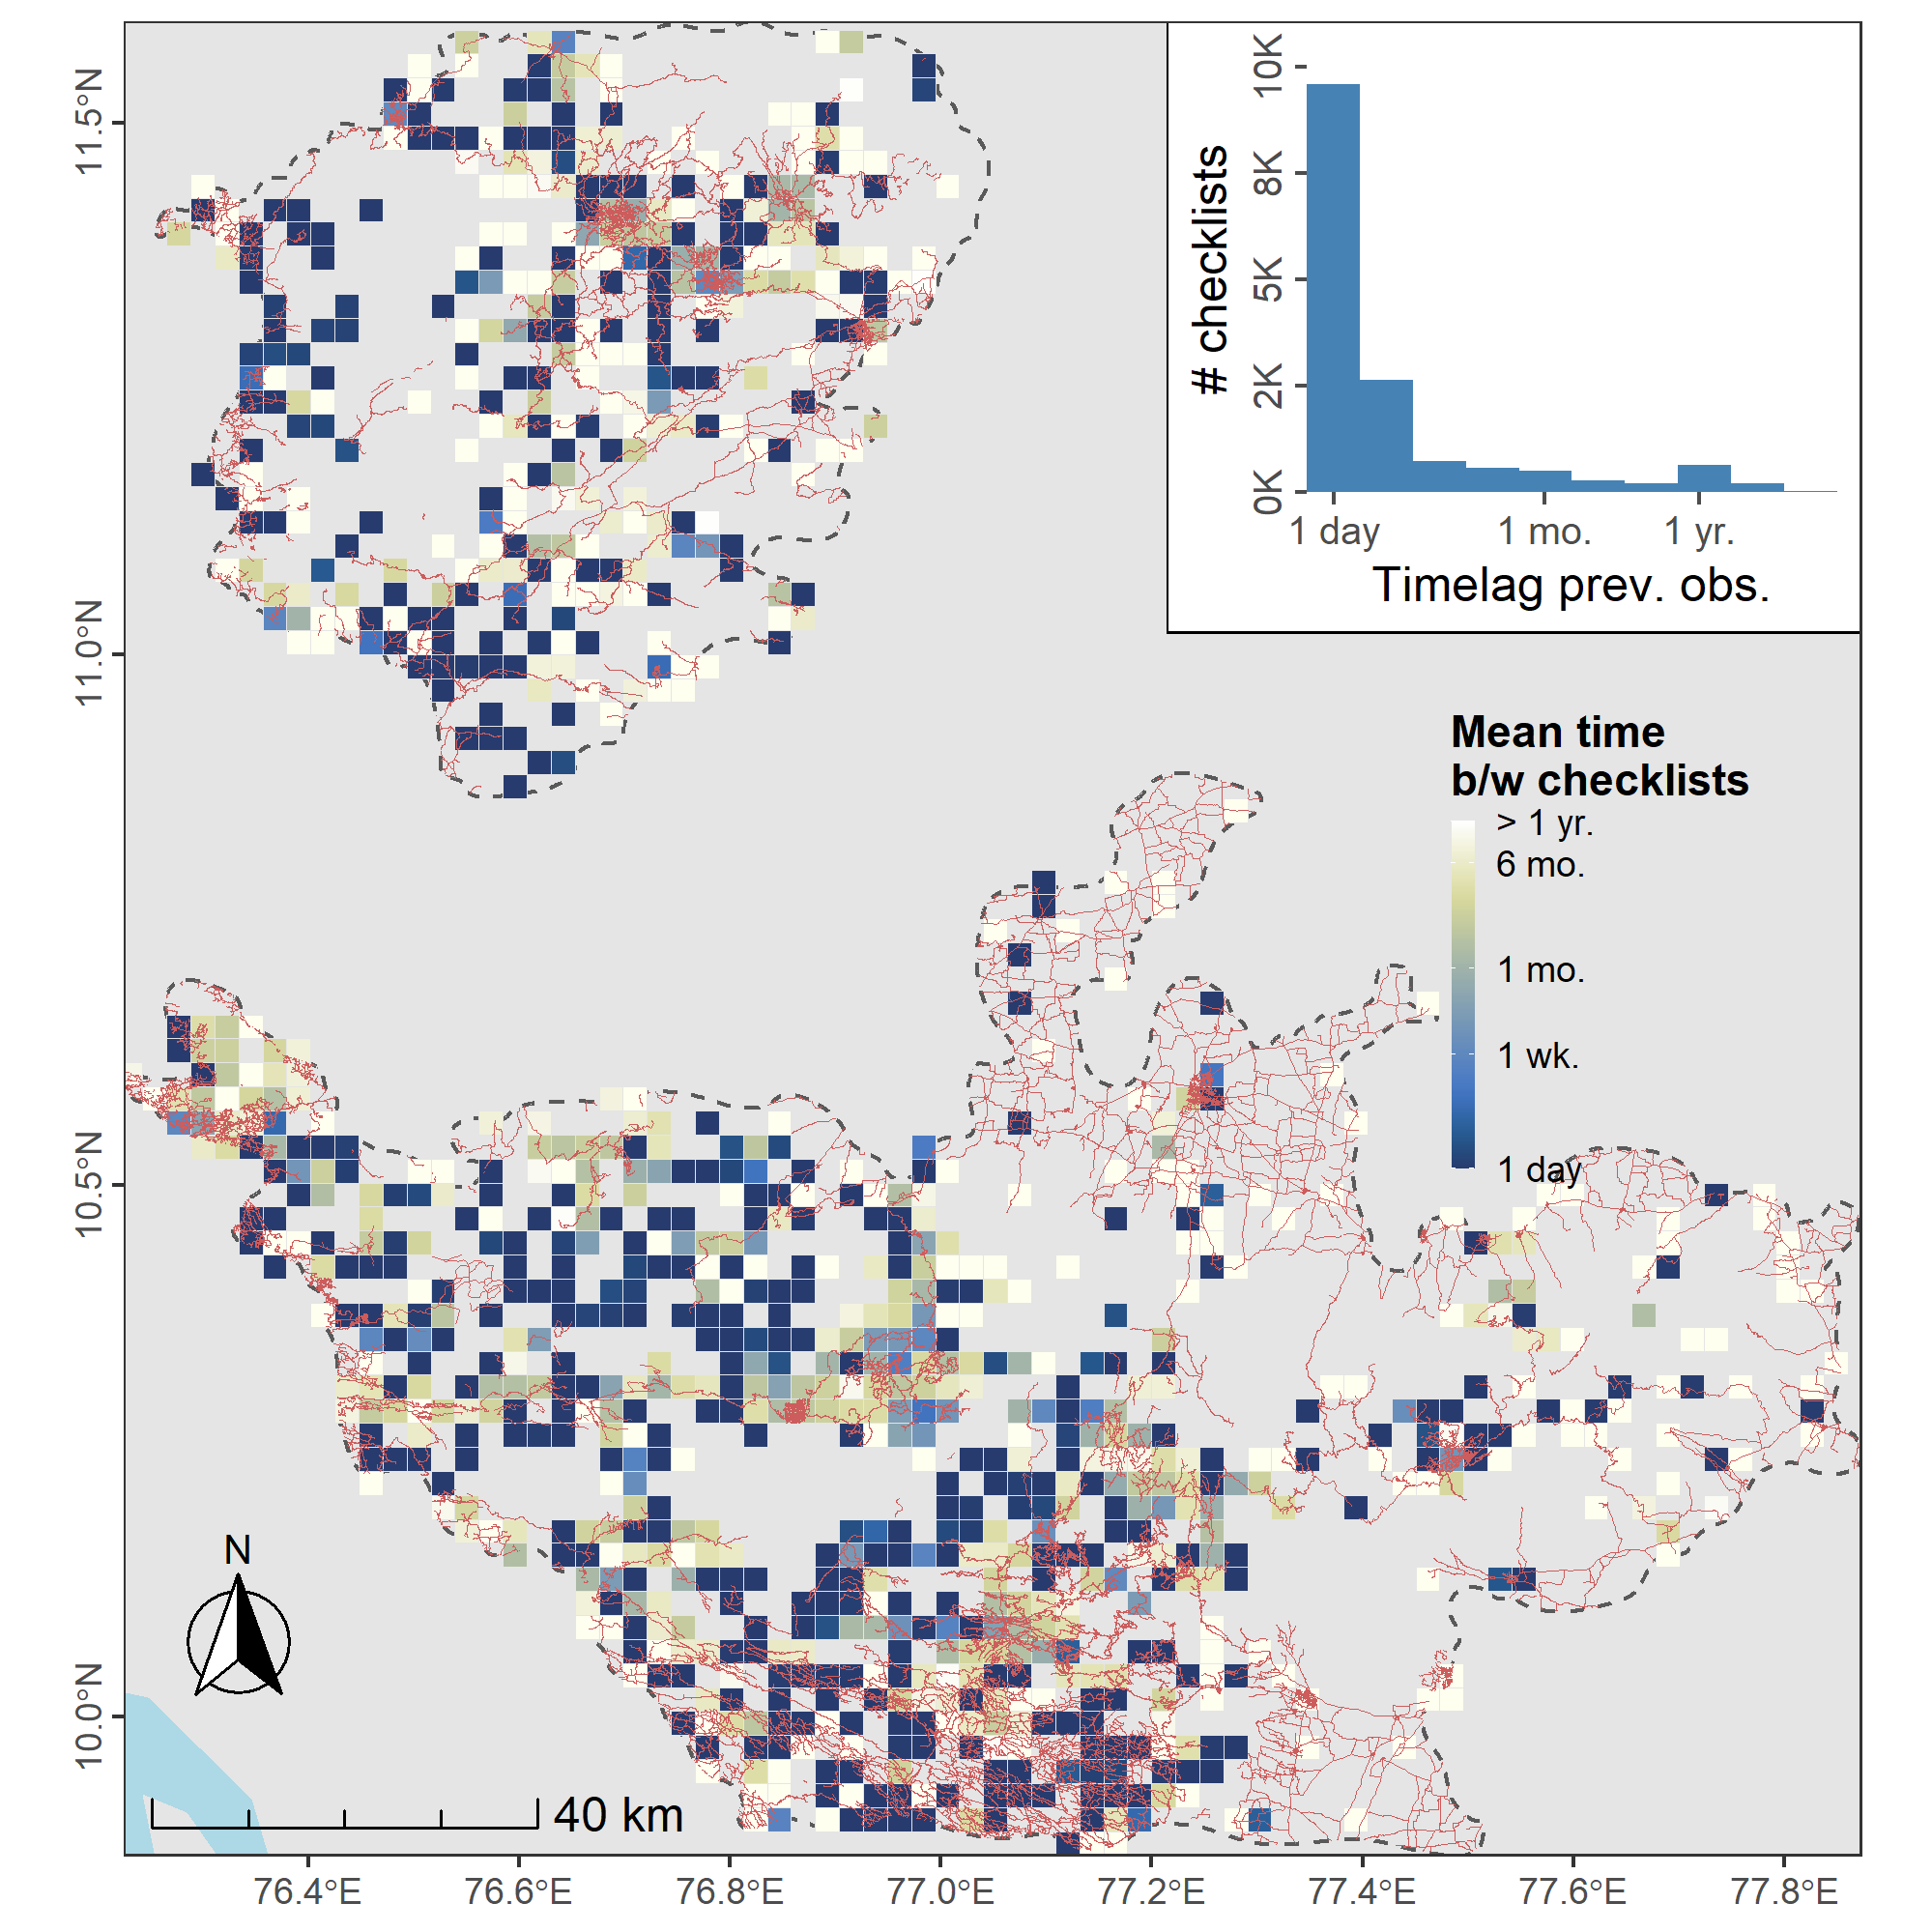
\includegraphics{figs/fig_temporal_bias.png}
\caption{Most sites are resurveyed at least once, but some are visited much more frequently than others. There does not appear to be a link between roads and visit frequency. eBird checklists are also strongly clustered in time, with some of the most sampled areas over the study period visited at intervals of \textgreater{} 1 week, and with some less intensively sampled areas visited frequently, at intervals of \textless{} 1 week. Overall, the majority of checklists are reported only a day after the previous checklist at that location (see inset).}
\end{figure}

\hypertarget{main-text-figure-3}{%
\subsection{Main Text Figure 3}\label{main-text-figure-3}}

Combining figures for spatial and temporal clustering into main text figure 3. This overall figure is not shown here, see main text.

\begin{Shaded}
\begin{Highlighting}[]
\CommentTok{# load spatial bias figure}
\KeywordTok{load}\NormalTok{(}\StringTok{"data/fig_checklists_grid.Rds"}\NormalTok{)}
\end{Highlighting}
\end{Shaded}

\begin{figure}
\centering
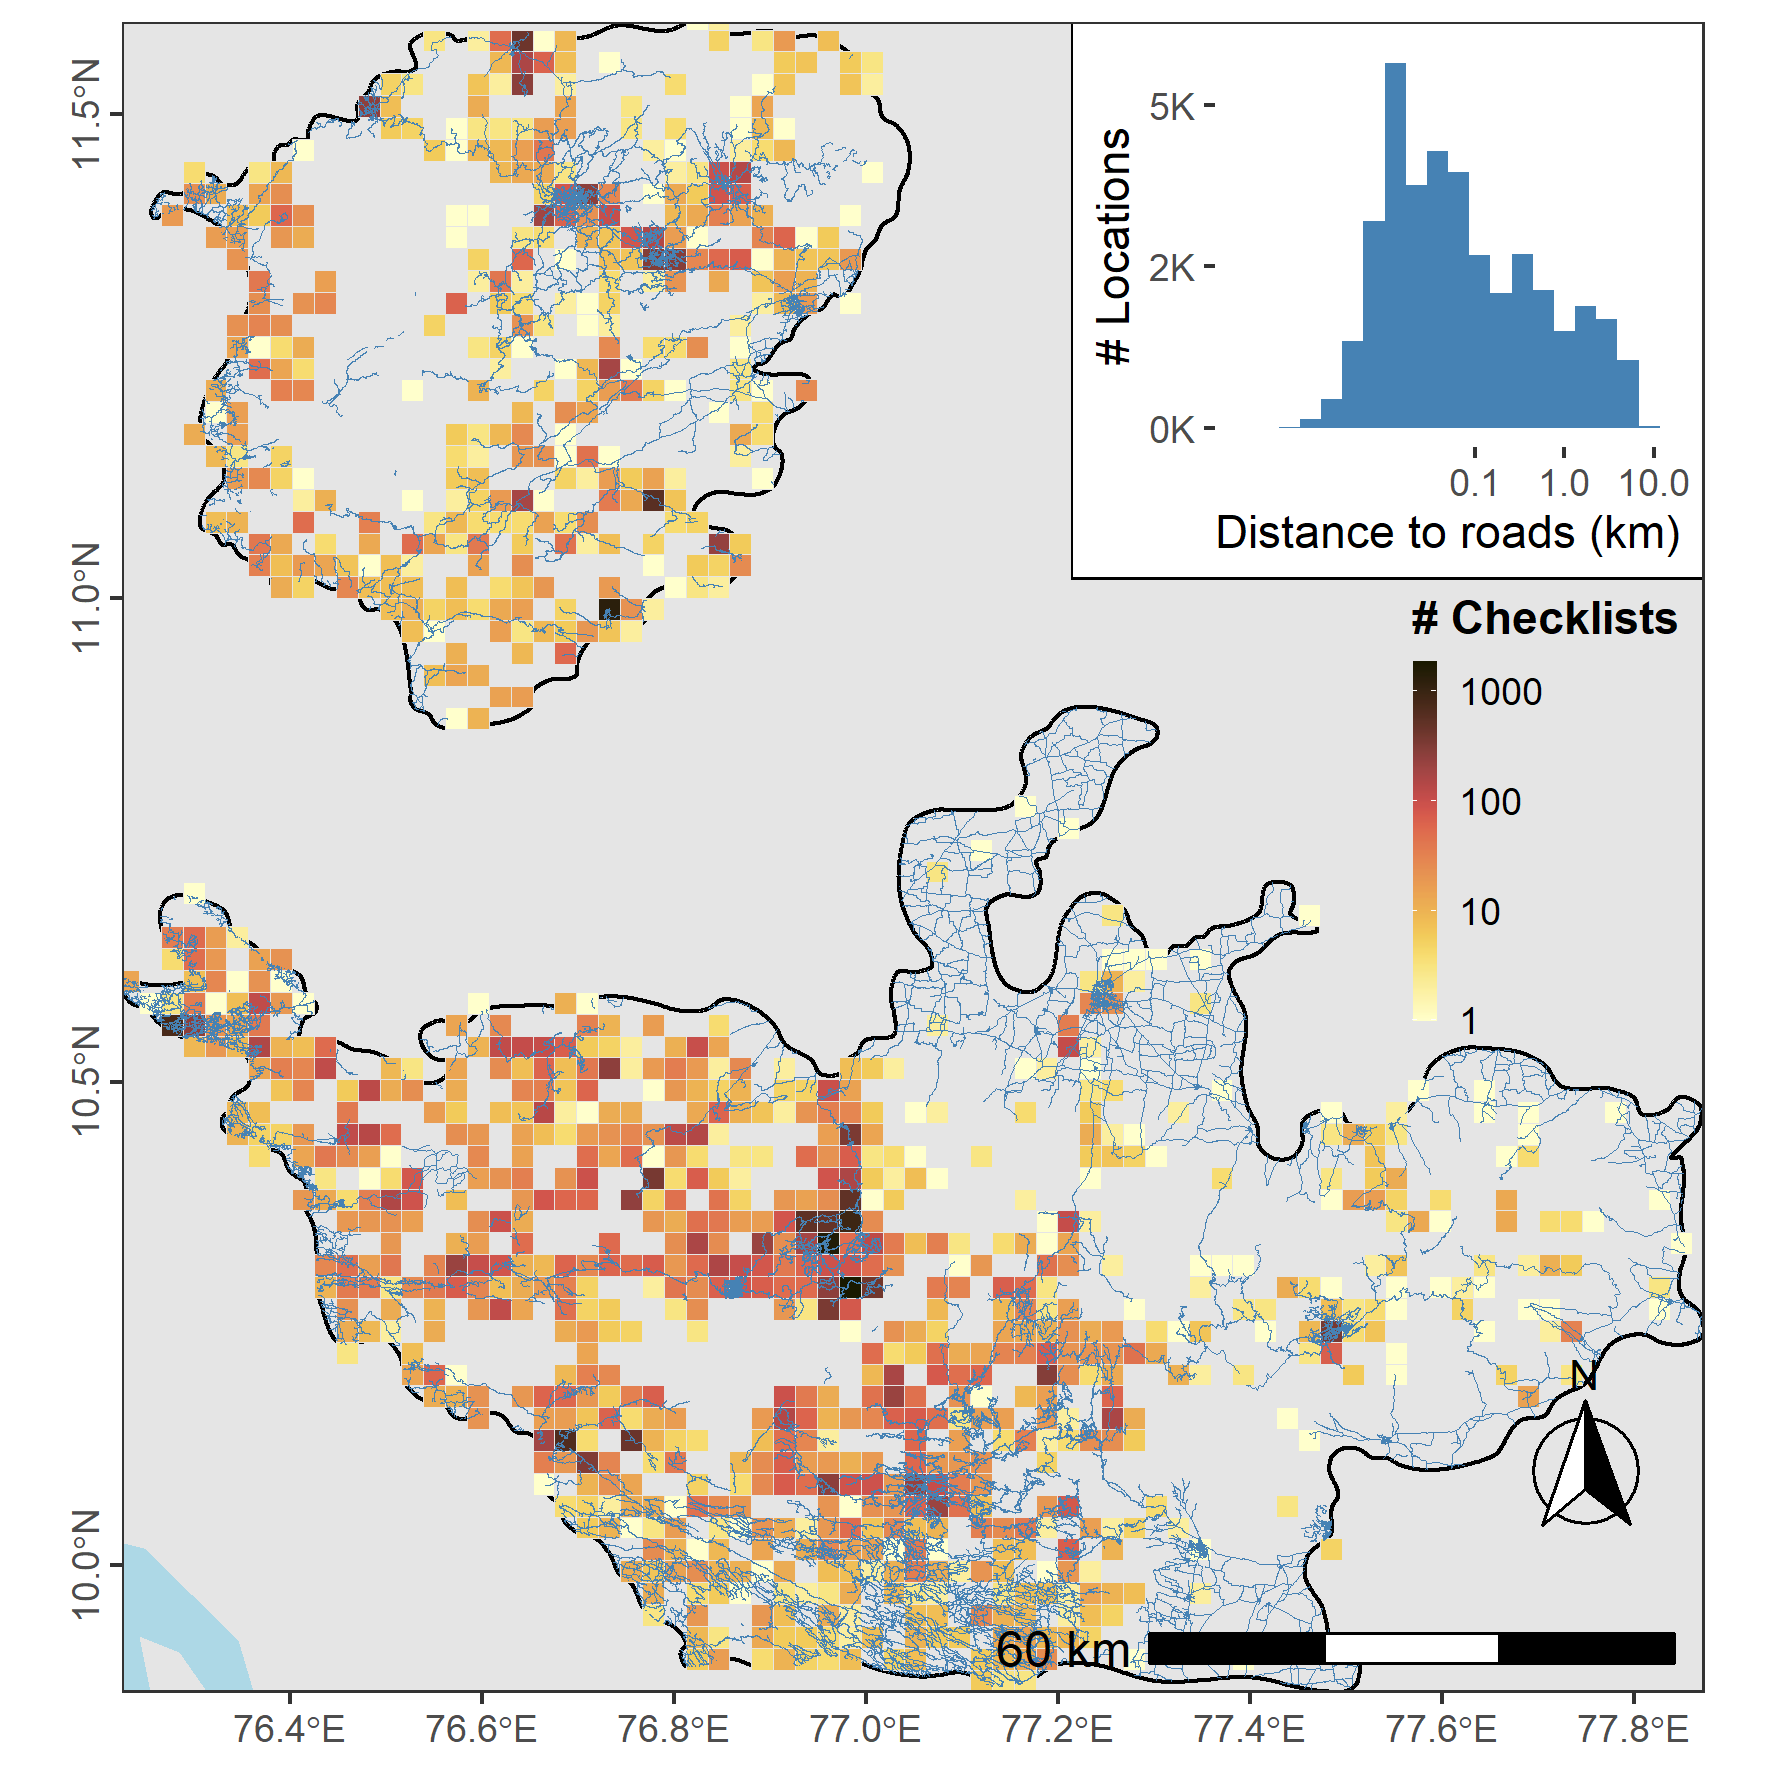
\includegraphics{figs/fig_03.png}
\caption{\textbf{Distribution of sampling effort in the form of eBird checklists in the Nilgiri and Anamalai Hills between 2013 and 2021.}
(a) Sampling effort across the Nilgiri and Anamalai Hills, in the form of eBird checklists reported by birdwatchers, mostly takes place along roads, with the majority of checklists located \textless1 km from a roadway (see distribution in inset), and therefore, only about 300m, on average, from the location of another checklist. (b) eBird checklists are also strongly clustered in time, with some of the most sampled areas over the study period visited at intervals of \textgreater{} 1 week, and with some less intensively sampled areas visited frequently, at intervals of \textless{} 1 week. Overall, most checklists are reported only a day after the previous checklist at that location (see inset). Both spatial and temporal clustering make data thinning necessary. Both panels show counts or mean intervals in a 2.5km grid cell; the study area is bounded by a dashed line, and roads within it are shown as (a) blue or (b) red lines.}
\end{figure}

\hypertarget{checklists-per-month}{%
\subsection{Checklists per Month}\label{checklists-per-month}}

We counted the checklists per month, pooled over years, to determine how sampling effort varies over the year.

\begin{Shaded}
\begin{Highlighting}[]
\CommentTok{# get two week period by date}
\NormalTok{data <-}\StringTok{ }\KeywordTok{select}\NormalTok{(data, X, Y, data)}

\CommentTok{# unnest}
\NormalTok{data <-}\StringTok{ }\KeywordTok{unnest}\NormalTok{(data, }\DataTypeTok{cols =} \StringTok{"data"}\NormalTok{)}

\CommentTok{# get fortnight}
\KeywordTok{library}\NormalTok{(lubridate)}
\NormalTok{data <-}\StringTok{ }\KeywordTok{mutate}\NormalTok{(data,}
  \DataTypeTok{week =} \KeywordTok{week}\NormalTok{(observation_date),}
  \DataTypeTok{week =}\NormalTok{ plyr}\OperatorTok{::}\KeywordTok{round_any}\NormalTok{(week, }\DecValTok{2}\NormalTok{),}
  \DataTypeTok{year =} \KeywordTok{year}\NormalTok{(observation_date),}
  \DataTypeTok{month =} \KeywordTok{month}\NormalTok{(observation_date)}
\NormalTok{)}

\CommentTok{# count checklists per fortnight}
\NormalTok{data_count <-}\StringTok{ }\KeywordTok{count}\NormalTok{(data, month, year)}
\end{Highlighting}
\end{Shaded}

\begin{figure}
\centering
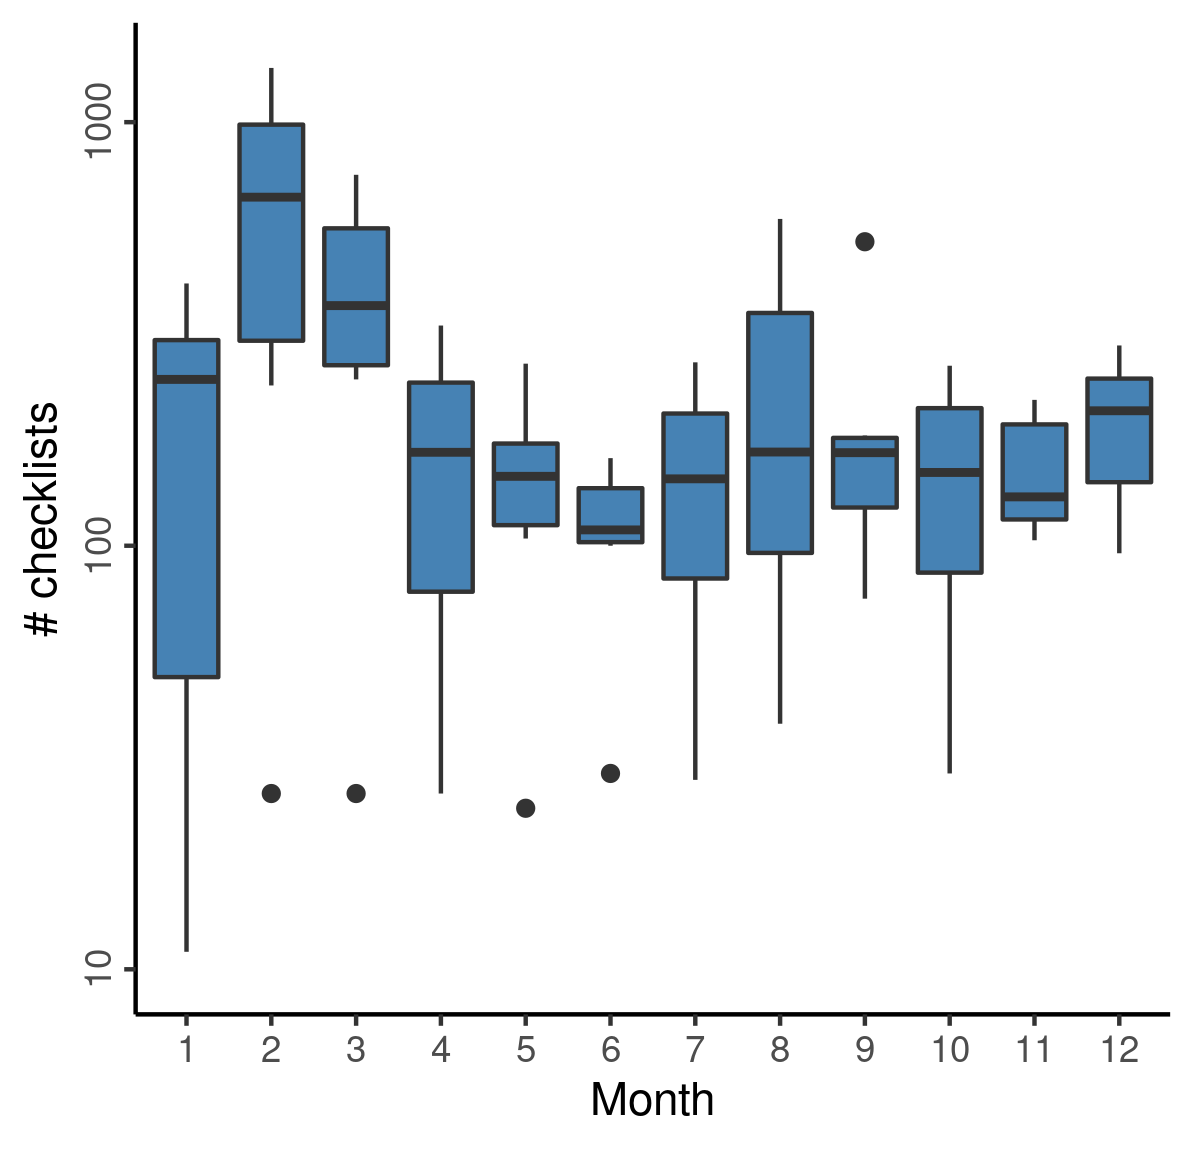
\includegraphics{figs/fig_chk_per_month.png}
\caption{Observations peak in the early months of the year, and decline towards the rainy months, slowly increasing until the following winter.}
\end{figure}

\hypertarget{adding-covariates-to-checklist-data}{%
\section{Adding Covariates to Checklist Data}\label{adding-covariates-to-checklist-data}}

In this section, we prepare a final list of covariates, after taking into account spatial sampling bias, temporal bias and observer expertise scores (examined in the previous section).

\hypertarget{prepare-libraries-and-data}{%
\subsection{Prepare libraries and data}\label{prepare-libraries-and-data}}

\begin{Shaded}
\begin{Highlighting}[]
\CommentTok{# load libs for data}
\KeywordTok{library}\NormalTok{(dplyr)}
\KeywordTok{library}\NormalTok{(readr)}
\KeywordTok{library}\NormalTok{(stringr)}
\KeywordTok{library}\NormalTok{(purrr)}
\KeywordTok{library}\NormalTok{(glue)}
\KeywordTok{library}\NormalTok{(tidyr)}

\CommentTok{# check for velox and install}
\KeywordTok{library}\NormalTok{(devtools)}
\ControlFlowTok{if}\NormalTok{ (}\OperatorTok{!}\StringTok{"velox"} \OperatorTok\StringTok{ }\KeywordTok{installed.packages}\NormalTok{()) \{}
  \KeywordTok{install_github}\NormalTok{(}\StringTok{"hunzikp/velox"}\NormalTok{)}
\NormalTok{\}}

\CommentTok{# load spatial}
\KeywordTok{library}\NormalTok{(raster)}
\KeywordTok{library}\NormalTok{(rgeos)}
\KeywordTok{library}\NormalTok{(velox)}
\KeywordTok{library}\NormalTok{(sf)}

\CommentTok{# load saved data object}
\KeywordTok{load}\NormalTok{(}\StringTok{"data/01_data_prelim_processing.rdata"}\NormalTok{)}
\end{Highlighting}
\end{Shaded}

\hypertarget{spatial-subsampling}{%
\subsection{Spatial subsampling}\label{spatial-subsampling}}

Sampling bias can be introduced into citizen science due to the often ad-hoc nature of data collection (Sullivan et al. \protect\hyperlink{ref-sullivan2014}{2014}). For eBird, this translates into checklists reported when convenient, rather than at regular or random points in time and space, leading to non-independence in the data if observations are spatio-temporally clustered (Johnston et al. \protect\hyperlink{ref-johnston2019a}{2019}). Spatio-temporal autocorrelation in the data can be reduced by sub-sampling at an appropriate spatial resolution, and by avoiding temporal clustering. We estimated two simple measures of spatial clustering: the distance from each site to the nearest road (road data from OpenStreetMap; (OpenStreetMap contributors \protect\hyperlink{ref-OpenStreetMap}{2019})), and the nearest-neighbor distance for each site. Sites were strongly tied to roads (mean distance to road ± SD = 390.77 ± 859.15 m; range = 0.28 m -- 7.64 km) and were on average only 297 m away from another site (SD = 553 m; range = 0.14 m -- 12.85 km) (Figure 3). This analysis was done in the previous section.

Here, to further reduce spatial autocorrelation, we divided the study area into a grid of 1km wide square cells and picked checklists from one site at random within each grid cell.

\begin{Shaded}
\begin{Highlighting}[]
\CommentTok{# grid based spatial thinning}
\NormalTok{gridsize <-}\StringTok{ }\DecValTok{500} \CommentTok{# grid size in metres}
\NormalTok{effort_distance_max <-}\StringTok{ }\DecValTok{1000} \CommentTok{# removing checklists with this distance}

\CommentTok{# make grids across the study site}
\NormalTok{hills <-}\StringTok{ }\KeywordTok{st_read}\NormalTok{(}\StringTok{"data/spatial/hillsShapefile/Nil_Ana_Pal.shp"}\NormalTok{) }\OperatorTok
\StringTok{  }\KeywordTok{st_transform}\NormalTok{(}\DecValTok{32643}\NormalTok{)}
\NormalTok{grid <-}\StringTok{ }\KeywordTok{st_make_grid}\NormalTok{(hills, }\DataTypeTok{cellsize =}\NormalTok{ gridsize)}

\CommentTok{# filtering on !pres_abs keeps absences}
\CommentTok{# this absence data will be thinned}
\NormalTok{data_thin_absences <-}\StringTok{ }\KeywordTok{filter}\NormalTok{(dataGrouped, }\OperatorTok{!}\NormalTok{pres_abs)}
\NormalTok{data_presences <-}\StringTok{ }\KeywordTok{filter}\NormalTok{(dataGrouped, pres_abs)}

\CommentTok{# split data by species}
\NormalTok{data_thin_absences <-}\StringTok{ }\KeywordTok{split}\NormalTok{(}
  \DataTypeTok{x =}\NormalTok{ data_thin_absences,}
  \DataTypeTok{f =}\NormalTok{ data_thin_absences}\OperatorTok{$}\NormalTok{scientific_name}
\NormalTok{)}
\end{Highlighting}
\end{Shaded}

\hypertarget{counting-presence-observation-proportion}{%
\subsubsection{Counting presence observation proportion}\label{counting-presence-observation-proportion}}

\begin{Shaded}
\begin{Highlighting}[]
\NormalTok{data_presence_prop <-}\StringTok{ }\KeywordTok{count}\NormalTok{(data_presences, scientific_name, }\DataTypeTok{name =} \StringTok{"presences"}\NormalTok{) }\OperatorTok
\StringTok{  }\KeywordTok{mutate}\NormalTok{(}
    \DataTypeTok{absences =} \KeywordTok{map_int}\NormalTok{(data_thin_absences, nrow),}
    \DataTypeTok{presence_prop =}\NormalTok{ presences }\OperatorTok{/}\StringTok{ }\NormalTok{(presences }\OperatorTok{+}\StringTok{ }\NormalTok{absences)}
\NormalTok{  )}

\CommentTok{# mean and sd of presence prop}
\NormalTok{data_presence_prop }\OperatorTok
\StringTok{  }\KeywordTok{summarise}\NormalTok{(}\KeywordTok{mean}\NormalTok{(presence_prop), }\KeywordTok{sd}\NormalTok{(presence_prop))}
\end{Highlighting}
\end{Shaded}

\begin{Shaded}
\begin{Highlighting}[]
\CommentTok{# spatial thinning on each species retains}
\CommentTok{# site with maximum visits per grid cell}
\NormalTok{data_thin_absences <-}\StringTok{ }\KeywordTok{map}\NormalTok{(data_thin_absences, }\ControlFlowTok{function}\NormalTok{(df) \{}

  \CommentTok{# count visits per locality}
\NormalTok{  df <-}\StringTok{ }\KeywordTok{group_by}\NormalTok{(df, locality) }\OperatorTok
\StringTok{    }\KeywordTok{mutate}\NormalTok{(}\DataTypeTok{tot_effort =} \KeywordTok{length}\NormalTok{(sampling_event_identifier)) }\OperatorTok
\StringTok{    }\KeywordTok{ungroup}\NormalTok{()}

  \CommentTok{# remove sites with distances above spatial independence}
\NormalTok{  df <-}\StringTok{ }\NormalTok{df }\OperatorTok
\StringTok{    }\NormalTok{dplyr}\OperatorTok{::}\KeywordTok{filter}\NormalTok{(effort_distance_km }\OperatorTok{<=}\StringTok{ }\NormalTok{effort_distance_max) }\OperatorTok
\StringTok{    }\KeywordTok{st_as_sf}\NormalTok{(}\DataTypeTok{coords =} \KeywordTok{c}\NormalTok{(}\StringTok{"longitude"}\NormalTok{, }\StringTok{"latitude"}\NormalTok{)) }\OperatorTok
\StringTok{    `}\DataTypeTok{st_crs<-}\StringTok{`}\NormalTok{(}\DecValTok{4326}\NormalTok{)}

  \CommentTok{# transform to regional UTM 43N and add id}
\NormalTok{  df <-}\StringTok{ }\NormalTok{df }\OperatorTok
\StringTok{    }\KeywordTok{st_transform}\NormalTok{(}\DecValTok{32643}\NormalTok{) }\OperatorTok
\StringTok{    }\KeywordTok{mutate}\NormalTok{(}\DataTypeTok{coordId =} \DecValTok{1}\OperatorTok{:}\KeywordTok{nrow}\NormalTok{(.)) }\OperatorTok
\StringTok{    }\KeywordTok{bind_cols}\NormalTok{(}\KeywordTok{as_tibble}\NormalTok{(}\KeywordTok{st_coordinates}\NormalTok{(.)))}

  \CommentTok{# whcih cell has which coords}
\NormalTok{  grid_overlap <-}\StringTok{ }\KeywordTok{st_contains}\NormalTok{(grid, df) }\OperatorTok
\StringTok{    }\KeywordTok{unclass}\NormalTok{() }\OperatorTok
\StringTok{    }\NormalTok{purrr}\OperatorTok{::}\KeywordTok{discard}\NormalTok{(}\DataTypeTok{.p =}\NormalTok{ is_empty)}

  \CommentTok{# count length of grid overlap list}
  \CommentTok{# this is the number of cells with points in them}
\NormalTok{  sampled_cells <-}\StringTok{ }\KeywordTok{length}\NormalTok{(grid_overlap)}

  \CommentTok{# make tibble}
\NormalTok{  grid_overlap <-}\StringTok{ }\KeywordTok{tibble}\NormalTok{(}
    \DataTypeTok{uid_cell =} \KeywordTok{seq}\NormalTok{(}\KeywordTok{length}\NormalTok{(grid_overlap)), }\CommentTok{# the uid_cell is specific to this sp.}
    \DataTypeTok{coordId =}\NormalTok{ grid_overlap}
\NormalTok{  )}

  \CommentTok{# unnest}
\NormalTok{  grid_overlap <-}\StringTok{ }\KeywordTok{unnest}\NormalTok{(grid_overlap, }\DataTypeTok{cols =} \StringTok{"coordId"}\NormalTok{)}

  \CommentTok{# join grid cell overlap with coordinate data}
\NormalTok{  df <-}\StringTok{ }\KeywordTok{left_join}\NormalTok{(df,}
\NormalTok{    grid_overlap,}
    \DataTypeTok{by =} \StringTok{"coordId"}
\NormalTok{  ) }\OperatorTok
\StringTok{    }\KeywordTok{st_drop_geometry}\NormalTok{()}

  \CommentTok{# for each uid_cell, select coord where effort is max}
\NormalTok{  points_max <-}\StringTok{ }\NormalTok{df }\OperatorTok
\StringTok{    }\KeywordTok{group_by}\NormalTok{(uid_cell) }\OperatorTok
\StringTok{    }\NormalTok{dplyr}\OperatorTok{::}\KeywordTok{filter}\NormalTok{(tot_effort }\OperatorTok{==}\StringTok{ }\KeywordTok{max}\NormalTok{(tot_effort)) }\OperatorTok
\StringTok{    }\CommentTok{# there may be multiple rows with max effort, select first}
\StringTok{    }\NormalTok{dplyr}\OperatorTok{::}\KeywordTok{filter}\NormalTok{(}\KeywordTok{row_number}\NormalTok{() }\OperatorTok{==}\StringTok{ }\DecValTok{1}\NormalTok{)}

  \CommentTok{# check for number of samples}
\NormalTok{  assertthat}\OperatorTok{::}\KeywordTok{assert_that}\NormalTok{(}
\NormalTok{    assertthat}\OperatorTok{::}\KeywordTok{are_equal}\NormalTok{(sampled_cells, }\KeywordTok{nrow}\NormalTok{(points_max),}
      \DataTypeTok{msg =} \StringTok{"spatial thinning error: more samples than}\CharTok{\textbackslash{}\textbackslash{}}
\StringTok{                          sampled cells"}
\NormalTok{    )}
\NormalTok{  )}
  \CommentTok{# check that there is one sample per cell}
\NormalTok{  assertthat}\OperatorTok{::}\KeywordTok{assert_that}\NormalTok{(}
\NormalTok{    assertthat}\OperatorTok{::}\KeywordTok{are_equal}\NormalTok{(}
      \KeywordTok{max}\NormalTok{(}\KeywordTok{count}\NormalTok{(points_max, uid_cell)}\OperatorTok{$}\NormalTok{n), }\DecValTok{1}
\NormalTok{    )}
\NormalTok{  )}

  \CommentTok{# return data without UID cell and coordinate Id}
\NormalTok{  dplyr}\OperatorTok{::}\KeywordTok{select}\NormalTok{(}\KeywordTok{ungroup}\NormalTok{(points_max), }\OperatorTok{-}\NormalTok{uid_cell, }\OperatorTok{-}\NormalTok{coordId, }\OperatorTok{-}\NormalTok{tot_effort)}
\NormalTok{\})}

\CommentTok{# remove old data}
\KeywordTok{rm}\NormalTok{(dataGrouped)}
\end{Highlighting}
\end{Shaded}

\hypertarget{count-absences-after-spatial-thinning}{%
\subsubsection{Count absences after spatial thinning}\label{count-absences-after-spatial-thinning}}

\begin{Shaded}
\begin{Highlighting}[]
\NormalTok{data_presence_prop <-}\StringTok{ }\NormalTok{data_presence_prop }\OperatorTok
\StringTok{  }\KeywordTok{mutate}\NormalTok{(}
    \DataTypeTok{absences_sp_thin =} \KeywordTok{map_int}\NormalTok{(data_thin_absences, nrow)}
\NormalTok{  )}
\end{Highlighting}
\end{Shaded}

\hypertarget{temporal-subsampling}{%
\subsection{Temporal subsampling}\label{temporal-subsampling}}

Additionally, from each selected site, we randomly selected a maximum of 10 \textbf{absence} checklists, which reduced temporal clustering. We kept \textbf{all} presence checklists.

\begin{Shaded}
\begin{Highlighting}[]
\CommentTok{# subsample data for random 10 observations}
\NormalTok{dataSubsample <-}\StringTok{ }\KeywordTok{map}\NormalTok{(data_thin_absences, }\ControlFlowTok{function}\NormalTok{(df) \{}
\NormalTok{  df <-}\StringTok{ }\KeywordTok{ungroup}\NormalTok{(df)}
\NormalTok{  df_to_locality <-}\StringTok{ }\KeywordTok{split}\NormalTok{(}\DataTypeTok{x =}\NormalTok{ df, }\DataTypeTok{f =}\NormalTok{ df}\OperatorTok{$}\NormalTok{locality)}
\NormalTok{  df_samples <-}\StringTok{ }\KeywordTok{map_if}\NormalTok{(}
    \DataTypeTok{.x =}\NormalTok{ df_to_locality,}
    \DataTypeTok{.p =} \ControlFlowTok{function}\NormalTok{(x) \{}
      \KeywordTok{nrow}\NormalTok{(x) }\OperatorTok{>}\StringTok{ }\DecValTok{10}
\NormalTok{    \},}
    \DataTypeTok{.f =} \ControlFlowTok{function}\NormalTok{(x) }\KeywordTok{sample_n}\NormalTok{(x, }\DecValTok{10}\NormalTok{, }\DataTypeTok{replace =} \OtherTok{FALSE}\NormalTok{)}
\NormalTok{  )}

  \KeywordTok{bind_rows}\NormalTok{(df_samples)}
\NormalTok{\})}
\end{Highlighting}
\end{Shaded}

\hypertarget{count-absences-after-temporal-thinning}{%
\subsubsection{Count absences after temporal thinning}\label{count-absences-after-temporal-thinning}}

\begin{Shaded}
\begin{Highlighting}[]
\NormalTok{data_presence_prop <-}\StringTok{ }\NormalTok{data_presence_prop }\OperatorTok
\StringTok{  }\KeywordTok{mutate}\NormalTok{(}
    \DataTypeTok{absences_tmp_thin =} \KeywordTok{map_int}\NormalTok{(dataSubsample, nrow),}
    \DataTypeTok{presence_prop_post_thin =}\NormalTok{ presences }\OperatorTok{/}\StringTok{ }\NormalTok{(presences }\OperatorTok{+}\StringTok{ }\NormalTok{absences_tmp_thin)}
\NormalTok{  )}

\CommentTok{# save data}
\KeywordTok{write_csv}\NormalTok{(data_presence_prop, }\StringTok{"data/results/data_class_balance.csv"}\NormalTok{)}
\end{Highlighting}
\end{Shaded}

\begin{Shaded}
\begin{Highlighting}[]
\CommentTok{# bind all spatially and temporally thinned absences rows for data frame}
\NormalTok{dataSubsample <-}\StringTok{ }\KeywordTok{bind_rows}\NormalTok{(dataSubsample)}

\CommentTok{# convert presence data to UTM 43 N and long-lat to X-Y}
\NormalTok{data_presences <-}\StringTok{ }\KeywordTok{bind_cols}\NormalTok{(}
\NormalTok{  data_presences,}
  \KeywordTok{as_tibble}\NormalTok{(}
    \KeywordTok{st_as_sf}\NormalTok{(}
\NormalTok{      data_presences,}
      \DataTypeTok{coords =} \KeywordTok{c}\NormalTok{(}\StringTok{"longitude"}\NormalTok{, }\StringTok{"latitude"}\NormalTok{),}
      \DataTypeTok{crs =} \DecValTok{4326}
\NormalTok{    ) }\OperatorTok
\StringTok{      }\KeywordTok{st_transform}\NormalTok{(}\DecValTok{32643}\NormalTok{) }\OperatorTok
\StringTok{      }\KeywordTok{st_coordinates}\NormalTok{()}
\NormalTok{  )}
\NormalTok{)}

\CommentTok{# drop long lat}
\NormalTok{data_presences <-}\StringTok{ }\NormalTok{dplyr}\OperatorTok{::}\KeywordTok{select}\NormalTok{(data_presences, }\OperatorTok{-}\NormalTok{longitude, }\OperatorTok{-}\NormalTok{latitude)}

\CommentTok{# join ALL PRESENCES and THINNED ABSENCES}
\NormalTok{dataSubsample <-}\StringTok{ }\KeywordTok{bind_rows}\NormalTok{(dataSubsample, data_presences)}

\CommentTok{# check joined data}
\NormalTok{assertthat}\OperatorTok{::}\KeywordTok{assert_that}\NormalTok{(}
  \KeywordTok{max}\NormalTok{(}\KeywordTok{apply}\NormalTok{(dataSubsample, }\DecValTok{2}\NormalTok{, }\ControlFlowTok{function}\NormalTok{(x) }\KeywordTok{sum}\NormalTok{(}\KeywordTok{is.na}\NormalTok{(x)))) }\OperatorTok{==}\StringTok{ }\DecValTok{0}\NormalTok{,}
  \DataTypeTok{msg =} \StringTok{"some columns missing from one of the datasets"}
\NormalTok{)}

\CommentTok{# remove previous data}
\KeywordTok{rm}\NormalTok{(data_thin_absences)}
\end{Highlighting}
\end{Shaded}

\hypertarget{add-checklist-calibration-index}{%
\subsection{Add checklist calibration index}\label{add-checklist-calibration-index}}

Load the CCI computed in the previous section. The CCI was the lone observer's expertise score for single-observer checklists, and the highest expertise score among observers for group checklists.

\begin{Shaded}
\begin{Highlighting}[]
\CommentTok{# read in obs score and extract numbers}
\NormalTok{expertiseScore <-}\StringTok{ }\KeywordTok{read_csv}\NormalTok{(}\StringTok{"data/03_data-obsExpertise-score.csv"}\NormalTok{) }\OperatorTok
\StringTok{  }\KeywordTok{mutate}\NormalTok{(}\DataTypeTok{numObserver =} \KeywordTok{str_extract}\NormalTok{(observer, }\StringTok{"}\CharTok{\textbackslash{}\textbackslash{}}\StringTok{d+"}\NormalTok{)) }\OperatorTok
\StringTok{  }\NormalTok{dplyr}\OperatorTok{::}\KeywordTok{select}\NormalTok{(}\OperatorTok{-}\NormalTok{observer)}

\CommentTok{# group seis consist of multiple observers}
\CommentTok{# in this case, seis need to have the highest expertise observer score}
\CommentTok{# as the associated covariate}

\CommentTok{# get unique observers per sei}
\NormalTok{dataSeiScore <-}\StringTok{ }\KeywordTok{distinct}\NormalTok{(}
\NormalTok{  dataSubsample, sampling_event_identifier,}
\NormalTok{  observer_id}
\NormalTok{) }\OperatorTok
\StringTok{  }\CommentTok{# make list column of observers}
\StringTok{  }\KeywordTok{mutate}\NormalTok{(}\DataTypeTok{observers =} \KeywordTok{str_split}\NormalTok{(observer_id, }\StringTok{","}\NormalTok{)) }\OperatorTok
\StringTok{  }\KeywordTok{unnest}\NormalTok{(}\DataTypeTok{cols =} \KeywordTok{c}\NormalTok{(observers)) }\OperatorTok
\StringTok{  }\CommentTok{# add numeric observer id}
\StringTok{  }\KeywordTok{mutate}\NormalTok{(}\DataTypeTok{numObserver =} \KeywordTok{str_extract}\NormalTok{(observers, }\StringTok{"}\CharTok{\textbackslash{}\textbackslash{}}\StringTok{d+"}\NormalTok{)) }\OperatorTok
\StringTok{  }\CommentTok{# now get distinct sei and observer id numeric}
\StringTok{  }\KeywordTok{distinct}\NormalTok{(sampling_event_identifier, numObserver)}

\CommentTok{# now add expertise score to sei}
\NormalTok{dataSeiScore <-}\StringTok{ }\KeywordTok{left_join}\NormalTok{(dataSeiScore, expertiseScore,}
  \DataTypeTok{by =} \StringTok{"numObserver"}
\NormalTok{) }\OperatorTok
\StringTok{  }\CommentTok{# get max expertise score per sei}
\StringTok{  }\KeywordTok{group_by}\NormalTok{(sampling_event_identifier) }\OperatorTok
\StringTok{  }\KeywordTok{summarise}\NormalTok{(}\DataTypeTok{expertise =} \KeywordTok{max}\NormalTok{(score))}

\CommentTok{# add to dataCovar}
\NormalTok{dataSubsample <-}\StringTok{ }\KeywordTok{left_join}\NormalTok{(dataSubsample, dataSeiScore,}
  \DataTypeTok{by =} \StringTok{"sampling_event_identifier"}
\NormalTok{)}

\CommentTok{# remove data without expertise score}
\NormalTok{dataSubsample <-}\StringTok{ }\KeywordTok{filter}\NormalTok{(dataSubsample, }\OperatorTok{!}\KeywordTok{is.na}\NormalTok{(expertise))}
\end{Highlighting}
\end{Shaded}

\hypertarget{add-climatic-and-landscape-covariates}{%
\subsection{Add climatic and landscape covariates}\label{add-climatic-and-landscape-covariates}}

Reload climate and land cover predictors prepared previously.

\begin{Shaded}
\begin{Highlighting}[]
\CommentTok{# list landscape covariate stacks}
\NormalTok{landscape_files <-}\StringTok{ "data/spatial/landscape_resamp01_km.tif"}

\CommentTok{# read in as stacks}
\NormalTok{landscape_data <-}\StringTok{ }\KeywordTok{stack}\NormalTok{(landscape_files)}

\CommentTok{# get proper names}
\NormalTok{elev_names <-}\StringTok{ }\KeywordTok{c}\NormalTok{(}\StringTok{"elev"}\NormalTok{, }\StringTok{"slope"}\NormalTok{, }\StringTok{"aspect"}\NormalTok{)}
\NormalTok{chelsa_names <-}\StringTok{ }\KeywordTok{c}\NormalTok{(}\StringTok{"bio_1"}\NormalTok{, }\StringTok{"bio_12"}\NormalTok{)}

\KeywordTok{names}\NormalTok{(landscape_data) <-}\StringTok{ }\KeywordTok{as.character}\NormalTok{(}\KeywordTok{glue}\NormalTok{(}\StringTok{'\{c(elev_names, chelsa_names, "landcover")\}'}\NormalTok{))}
\end{Highlighting}
\end{Shaded}

\hypertarget{spatial-buffers-around-selected-checklists}{%
\subsection{Spatial buffers around selected checklists}\label{spatial-buffers-around-selected-checklists}}

Every checklist on eBird is associated with a latitude and longitude. However, the coordinates entered by an observer may not accurately depict the location at which a species was detected. This can occur for two reasons: first, traveling checklists are often associated with a single location along the route travelled by observers; and second, checklist locations could be assigned to a `hotspot' -- a location that is marked by eBird as being frequented by multiple observers. In many cases, an observation might be assigned to a hotspot even though the observation was not made at the precise location of the hotspot (J. \protect\hyperlink{ref-praveenj.2017}{2017}). Johnston et al., (2019) showed that a large proportion of observations occurred within a 3km grid, even for those checklists up to 5km in length. Hence to adjust for spatial precision, we considered a minimum radius of 2.5km around each unique locality when sampling environmental covariate values.

\begin{Shaded}
\begin{Highlighting}[]
\CommentTok{# assign neighbourhood radius in m}
\NormalTok{sample_radius <-}\StringTok{ }\FloatTok{2.5} \OperatorTok{*}\StringTok{ }\FloatTok{1e3}

\CommentTok{# get distinct points and make buffer}
\NormalTok{ebird_buff <-}\StringTok{ }\NormalTok{dataSubsample }\OperatorTok
\StringTok{  }\KeywordTok{ungroup}\NormalTok{() }\OperatorTok
\StringTok{  }\KeywordTok{distinct}\NormalTok{(X, Y) }\OperatorTok
\StringTok{  }\CommentTok{# remove NAs}
\StringTok{  }\KeywordTok{drop_na}\NormalTok{()}

\CommentTok{# convert to spatial features}
\NormalTok{ebird_buff <-}\StringTok{ }\KeywordTok{st_as_sf}\NormalTok{(ebird_buff, }\DataTypeTok{coords =} \KeywordTok{c}\NormalTok{(}\StringTok{"X"}\NormalTok{, }\StringTok{"Y"}\NormalTok{), }\DataTypeTok{crs =} \DecValTok{32643}\NormalTok{) }\OperatorTok
\StringTok{  }\CommentTok{# add long lat}
\StringTok{  }\KeywordTok{bind_cols}\NormalTok{(}\KeywordTok{as_tibble}\NormalTok{(}\KeywordTok{st_coordinates}\NormalTok{(.))) }\OperatorTok
\StringTok{  }\CommentTok{# make buffer around points}
\StringTok{  }\KeywordTok{st_buffer}\NormalTok{(}\DataTypeTok{dist =}\NormalTok{ sample_radius)}
\end{Highlighting}
\end{Shaded}

\hypertarget{spatial-buffer-wide-covariates}{%
\subsection{Spatial buffer-wide covariates}\label{spatial-buffer-wide-covariates}}

\hypertarget{mean-climatic-covariates}{%
\subsubsection{Mean climatic covariates}\label{mean-climatic-covariates}}

All climatic covariates are sampled by considering the mean values within a 2.5km radius as discussed above and prefixed ``am\_''.

\begin{Shaded}
\begin{Highlighting}[]
\CommentTok{# get area mean for all preds except landcover, which is the last one}
\NormalTok{stk <-}\StringTok{ }\NormalTok{raster}\OperatorTok{::}\KeywordTok{dropLayer}\NormalTok{(landscape_data, }\StringTok{"landcover"}\NormalTok{) }\CommentTok{# removing landcover here}
\NormalTok{velstk <-}\StringTok{ }\KeywordTok{velox}\NormalTok{(stk)}

\CommentTok{# velox raster value extraction}
\NormalTok{dextr <-}\StringTok{ }\NormalTok{velstk}\OperatorTok{$}\KeywordTok{extract}\NormalTok{(}
  \DataTypeTok{sp =}\NormalTok{ ebird_buff, }\DataTypeTok{df =} \OtherTok{TRUE}\NormalTok{,}
  \DataTypeTok{fun =} \ControlFlowTok{function}\NormalTok{(x) }\KeywordTok{mean}\NormalTok{(x, }\DataTypeTok{na.rm =}\NormalTok{ T)}
\NormalTok{)}

\CommentTok{# assign names for joining}
\KeywordTok{names}\NormalTok{(dextr) <-}\StringTok{ }\KeywordTok{c}\NormalTok{(}\StringTok{"id"}\NormalTok{, }\KeywordTok{names}\NormalTok{(stk))}
\NormalTok{env_area_mean <-}\StringTok{ }\KeywordTok{as_tibble}\NormalTok{(dextr)}

\CommentTok{# add id to buffer data}
\NormalTok{ebird_buff <-}\StringTok{ }\KeywordTok{mutate}\NormalTok{(ebird_buff,}
  \DataTypeTok{id =} \KeywordTok{seq}\NormalTok{(}\KeywordTok{nrow}\NormalTok{(ebird_buff))}
\NormalTok{)}

\CommentTok{# join to buffer data}
\NormalTok{ebird_buff <-}\StringTok{ }\KeywordTok{inner_join}\NormalTok{(ebird_buff, env_area_mean)}
\end{Highlighting}
\end{Shaded}

\hypertarget{proportions-of-land-cover-type}{%
\subsubsection{Proportions of land cover type}\label{proportions-of-land-cover-type}}

All land cover covariates were sampled by considering the proportion of each land cover type within a 2.5km radius.

\begin{Shaded}
\begin{Highlighting}[]
\CommentTok{# get the last element of each stack from the list}
\CommentTok{# this is the landcover at that resolution}
\NormalTok{lc <-}\StringTok{ }\NormalTok{landscape_data[[}\StringTok{"landcover"}\NormalTok{]] }\CommentTok{# accessing landcover here}
\NormalTok{lc_velox <-}\StringTok{ }\KeywordTok{velox}\NormalTok{(lc)}
\NormalTok{lc_vals <-}\StringTok{ }\NormalTok{lc_velox}\OperatorTok{$}\KeywordTok{extract}\NormalTok{(}\DataTypeTok{sp =}\NormalTok{ ebird_buff, }\DataTypeTok{df =} \OtherTok{TRUE}\NormalTok{)}
\KeywordTok{names}\NormalTok{(lc_vals) <-}\StringTok{ }\KeywordTok{c}\NormalTok{(}\StringTok{"id"}\NormalTok{, }\StringTok{"lc"}\NormalTok{)}

\CommentTok{# get landcover proportions}
\NormalTok{lc_prop <-}\StringTok{ }\KeywordTok{count}\NormalTok{(lc_vals, id, lc) }\OperatorTok
\StringTok{  }\KeywordTok{group_by}\NormalTok{(id) }\OperatorTok
\StringTok{  }\KeywordTok{mutate}\NormalTok{(}
    \DataTypeTok{lc =} \KeywordTok{glue}\NormalTok{(}\StringTok{'lc_\{str_pad(lc, 2, pad = "0")\}'}\NormalTok{),}
    \DataTypeTok{prop =}\NormalTok{ n }\OperatorTok{/}\StringTok{ }\KeywordTok{sum}\NormalTok{(n)}
\NormalTok{  ) }\OperatorTok
\StringTok{  }\NormalTok{dplyr}\OperatorTok{::}\KeywordTok{select}\NormalTok{(}\OperatorTok{-}\NormalTok{n) }\OperatorTok
\StringTok{  }\NormalTok{tidyr}\OperatorTok{::}\KeywordTok{pivot_wider}\NormalTok{(}
    \DataTypeTok{names_from =}\NormalTok{ lc,}
    \DataTypeTok{values_from =}\NormalTok{ prop,}
    \DataTypeTok{values_fill =} \KeywordTok{list}\NormalTok{(}\DataTypeTok{prop =} \DecValTok{0}\NormalTok{)}
\NormalTok{  ) }\OperatorTok
\StringTok{  }\KeywordTok{ungroup}\NormalTok{()}

\CommentTok{# join to data}
\NormalTok{ebird_buff <-}\StringTok{ }\KeywordTok{mutate}\NormalTok{(ebird_buff, lc_prop)}
\end{Highlighting}
\end{Shaded}

\hypertarget{link-environmental-covariates-to-checklists}{%
\subsubsection{Link environmental covariates to checklists}\label{link-environmental-covariates-to-checklists}}

\begin{Shaded}
\begin{Highlighting}[]
\CommentTok{# drop geometry}
\NormalTok{ebird_buff <-}\StringTok{ }\KeywordTok{st_drop_geometry}\NormalTok{(ebird_buff)}

\CommentTok{# link to dataSubsample}
\NormalTok{dataSubsample <-}\StringTok{ }\KeywordTok{inner_join}\NormalTok{(dataSubsample, ebird_buff,}
  \DataTypeTok{by =} \KeywordTok{c}\NormalTok{(}\StringTok{"X"}\NormalTok{, }\StringTok{"Y"}\NormalTok{)}
\NormalTok{)}
\end{Highlighting}
\end{Shaded}

Save data to file.

\begin{Shaded}
\begin{Highlighting}[]
\CommentTok{# write to file}
\KeywordTok{write_csv}\NormalTok{(dataSubsample, }\DataTypeTok{path =} \KeywordTok{glue}\NormalTok{(}\StringTok{"data/04_data-covars-2.5km.csv"}\NormalTok{))}
\end{Highlighting}
\end{Shaded}

\hypertarget{modelling-species-occupancy}{%
\section{Modelling Species Occupancy}\label{modelling-species-occupancy}}

\hypertarget{load-necessary-libraries}{%
\subsubsection{Load necessary libraries}\label{load-necessary-libraries}}

\begin{Shaded}
\begin{Highlighting}[]
\CommentTok{# Load libraries}
\CommentTok{# for ebird data}
\KeywordTok{library}\NormalTok{(auk)}
\KeywordTok{library}\NormalTok{(ebirdst)}

\CommentTok{# general data}
\KeywordTok{library}\NormalTok{(tidyverse)}
\KeywordTok{library}\NormalTok{(data.table)}
\KeywordTok{library}\NormalTok{(lubridate)}
\KeywordTok{library}\NormalTok{(openxlsx)}
\KeywordTok{library}\NormalTok{(raster) }\CommentTok{# probably unnecessary}

\CommentTok{# for models}
\KeywordTok{library}\NormalTok{(unmarked)}
\KeywordTok{library}\NormalTok{(MuMIn)}
\KeywordTok{library}\NormalTok{(AICcmodavg)}
\KeywordTok{library}\NormalTok{(fields)}

\CommentTok{# for computation}
\KeywordTok{library}\NormalTok{(doParallel)}
\KeywordTok{library}\NormalTok{(snow)}
\KeywordTok{library}\NormalTok{(ecodist)}

\CommentTok{# Source necessary functions}
\KeywordTok{source}\NormalTok{(}\StringTok{"R/fun_screen_cor.R"}\NormalTok{)}
\KeywordTok{source}\NormalTok{(}\StringTok{"R/fun_model_estimate_collection.r"}\NormalTok{)}
\end{Highlighting}
\end{Shaded}

\hypertarget{load-dataframe-and-prepare-covariates}{%
\subsection{Load dataframe and prepare covariates}\label{load-dataframe-and-prepare-covariates}}

Here, we load the required dataframe that contains 10 random visits to a site and environmental covariates that were prepared at a spatial scale of 2.5 sq.km. We also scaled all covariates (mean around 0 and standard deviation of 1). Next, we ensured that only Traveling and Stationary checklists were considered. Even though stationary counts have no distance traveled, we defaulted all stationary accounts to an effective distance of 100m, which we consider the average maximum detection radius for most bird species in our area.

\begin{Shaded}
\begin{Highlighting}[]
\CommentTok{# Load in the prepared dataframe}
\NormalTok{dat <-}\StringTok{ }\KeywordTok{fread}\NormalTok{(}\StringTok{"data/04_data-covars-2.5km.csv"}\NormalTok{, }\DataTypeTok{header =}\NormalTok{ T)}
\NormalTok{dat <-}\StringTok{ }\KeywordTok{as_tibble}\NormalTok{(dat)}
\KeywordTok{head}\NormalTok{(dat)}
\end{Highlighting}
\end{Shaded}

\hypertarget{handle-the-sampling-protocol}{%
\subsubsection{Handle the sampling protocol}\label{handle-the-sampling-protocol}}

Select protocol and add 0.1 km to stationary checklists.

\begin{Shaded}
\begin{Highlighting}[]
\CommentTok{# Some more pre-processing to get the right data structures}

\CommentTok{# Ensuring that only Traveling and Stationary checklists were considered}
\KeywordTok{names}\NormalTok{(dat)}
\NormalTok{dat <-}\StringTok{ }\NormalTok{dat }\OperatorTok\StringTok{ }\KeywordTok{filter}\NormalTok{(protocol_type }\OperatorTok\StringTok{ }\KeywordTok{c}\NormalTok{(}\StringTok{"Traveling"}\NormalTok{, }\StringTok{"Stationary"}\NormalTok{))}

\CommentTok{# We take all stationary counts and give them a distance of 100 m (so 0.1 km),}
\CommentTok{# as that's approximately the max normal hearing distance for people doing point}
\CommentTok{# counts.}
\NormalTok{dat <-}\StringTok{ }\NormalTok{dat }\OperatorTok
\StringTok{  }\KeywordTok{mutate}\NormalTok{(}\DataTypeTok{effort_distance_km =} \KeywordTok{if_else}\NormalTok{(}
\NormalTok{    effort_distance_km }\OperatorTok{==}\StringTok{ }\DecValTok{0} \OperatorTok{&}
\StringTok{      }\NormalTok{protocol_type }\OperatorTok{==}\StringTok{ "Stationary"}\NormalTok{,}
    \FloatTok{0.1}\NormalTok{, effort_distance_km}
\NormalTok{  ))}
\end{Highlighting}
\end{Shaded}

\hypertarget{handle-time-and-date}{%
\subsubsection{Handle time and date}\label{handle-time-and-date}}

Convert time and date to julian date and minutes since day.

\begin{Shaded}
\begin{Highlighting}[]
\CommentTok{# Converting time observations started to numeric and adding it as a new column}
\CommentTok{# This new column will be minute_observations_started}
\NormalTok{dat <-}
\StringTok{  }\NormalTok{dat }\OperatorTok
\StringTok{  }\KeywordTok{mutate}\NormalTok{(}
    \DataTypeTok{min_obs_started =} \KeywordTok{as.integer}\NormalTok{(}
      \KeywordTok{as.difftime}\NormalTok{(}
\NormalTok{        time_observations_started,}
        \DataTypeTok{format =} \StringTok{"%H:%M:%S"}\NormalTok{, }\DataTypeTok{units =} \StringTok{"mins"}
\NormalTok{      )}
\NormalTok{    )}
\NormalTok{  )}

\CommentTok{# Adding the julian date to the dataframe}
\NormalTok{dat <-}\StringTok{ }\NormalTok{dat }\OperatorTok
\StringTok{  }\KeywordTok{mutate}\NormalTok{(}\DataTypeTok{julian_date =}\NormalTok{ lubridate}\OperatorTok{::}\KeywordTok{yday}\NormalTok{(observation_date))}

\CommentTok{# recode julian date to model it as a linear predictor}
\NormalTok{dat <-}\StringTok{ }\NormalTok{dat }\OperatorTok
\StringTok{  }\KeywordTok{mutate}\NormalTok{(}
    \DataTypeTok{newjulianDate =}
      \KeywordTok{case_when}\NormalTok{(}
\NormalTok{        (julian_date }\OperatorTok{>=}\StringTok{ }\DecValTok{334} \OperatorTok{&}\StringTok{ }\NormalTok{julian_date) }\OperatorTok{<=}\StringTok{ }\DecValTok{365} \OperatorTok{~}
\StringTok{        }\NormalTok{(julian_date }\OperatorTok{-}\StringTok{ }\DecValTok{333}\NormalTok{),}
\NormalTok{        (julian_date }\OperatorTok{>=}\StringTok{ }\DecValTok{1} \OperatorTok{&}\StringTok{ }\NormalTok{julian_date) }\OperatorTok{<=}\StringTok{ }\DecValTok{152} \OperatorTok{~}
\StringTok{        }\NormalTok{(julian_date }\OperatorTok{+}\StringTok{ }\DecValTok{31}\NormalTok{)}
\NormalTok{      )}
\NormalTok{  ) }\OperatorTok
\StringTok{  }\KeywordTok{drop_na}\NormalTok{(newjulianDate)}

\CommentTok{# recode time observations started to model it as a linear predictor}
\NormalTok{dat <-}\StringTok{ }\NormalTok{dat }\OperatorTok
\StringTok{  }\KeywordTok{mutate}\NormalTok{(}
    \DataTypeTok{newmin_obs_started =} \KeywordTok{case_when}\NormalTok{(}
\NormalTok{      min_obs_started }\OperatorTok{>=}\StringTok{ }\DecValTok{300} \OperatorTok{&}\StringTok{ }\NormalTok{min_obs_started }\OperatorTok{<=}\StringTok{ }\DecValTok{720} \OperatorTok{~}
\StringTok{      }\KeywordTok{abs}\NormalTok{(min_obs_started }\OperatorTok{-}\StringTok{ }\DecValTok{720}\NormalTok{),}
\NormalTok{      min_obs_started }\OperatorTok{>=}\StringTok{ }\DecValTok{720} \OperatorTok{&}\StringTok{ }\NormalTok{min_obs_started }\OperatorTok{<=}\StringTok{ }\DecValTok{1140} \OperatorTok{~}
\StringTok{      }\KeywordTok{abs}\NormalTok{(}\DecValTok{720} \OperatorTok{-}\StringTok{ }\NormalTok{min_obs_started)}
\NormalTok{    )}
\NormalTok{  ) }\OperatorTok
\StringTok{  }\KeywordTok{drop_na}\NormalTok{(newmin_obs_started)}
\end{Highlighting}
\end{Shaded}

\hypertarget{scaling-covariates}{%
\subsubsection{Scaling covariates}\label{scaling-covariates}}

\begin{Shaded}
\begin{Highlighting}[]
\CommentTok{# Removing other unnecessary columns from the dataframe and creating a clean one without the rest}
\KeywordTok{names}\NormalTok{(dat)}
\CommentTok{# select relevant columns BY NAME}
\NormalTok{dat <-}\StringTok{ }\NormalTok{dplyr}\OperatorTok{::}\KeywordTok{select}\NormalTok{(}
\NormalTok{  dat,}
  \KeywordTok{c}\NormalTok{(}
    \StringTok{"duration_minutes"}\NormalTok{, }\StringTok{"effort_distance_km"}\NormalTok{, }\StringTok{"locality"}\NormalTok{,}
    \StringTok{"locality_type"}\NormalTok{, }\StringTok{"locality_id"}\NormalTok{, }\StringTok{"observer_id"}\NormalTok{,}
    \StringTok{"observation_date"}\NormalTok{, }\StringTok{"scientific_name"}\NormalTok{, }\StringTok{"observation_count"}\NormalTok{,}
    \StringTok{"protocol_type"}\NormalTok{, }\StringTok{"number_observers"}\NormalTok{, }\StringTok{"pres_abs"}
\NormalTok{  ),}

  \CommentTok{# rename X-Y but }\AlertTok{NOTE}\CommentTok{ THEY ARE IN UTM COORDINATES}
  \DataTypeTok{longitude =} \StringTok{"X"}\NormalTok{, }\DataTypeTok{latitude =} \StringTok{"Y"}\NormalTok{,}
\NormalTok{  expertise,}

  \CommentTok{# elevation and climate layers}
\NormalTok{  elev, bio4, bio15,}

  \CommentTok{# all LANDCOVER COLUMNS}
  \KeywordTok{matches}\NormalTok{(}\StringTok{"lc"}\NormalTok{),}

  \CommentTok{# set new columns to old column names}
  \DataTypeTok{julian_date =} \StringTok{"newjulianDate"}\NormalTok{,}
  \DataTypeTok{min_obs_started =} \StringTok{"newmin_obs_started"}
\NormalTok{)}

\CommentTok{# add year and convert presence-absence to integer}
\NormalTok{dat}\FloatTok{.1}\NormalTok{ <-}\StringTok{ }\NormalTok{dat }\OperatorTok
\StringTok{  }\KeywordTok{mutate}\NormalTok{(}
    \DataTypeTok{year =} \KeywordTok{year}\NormalTok{(observation_date),}
    \DataTypeTok{pres_abs =} \KeywordTok{as.integer}\NormalTok{(pres_abs)}
\NormalTok{  ) }\CommentTok{# occupancy modeling requires an integer response}

\CommentTok{# Scaling detection and occupancy covariates}
\NormalTok{dat.scaled <-}\StringTok{ }\NormalTok{dat}\FloatTok{.1}

\CommentTok{# Note: Never refer to columns by numbers, numbers change, names remain}
\NormalTok{cols_to_scale <-}\StringTok{ }\KeywordTok{c}\NormalTok{(}
  \StringTok{"duration_minutes"}\NormalTok{, }\StringTok{"effort_distance_km"}\NormalTok{,}
  \StringTok{"number_observers"}\NormalTok{, }\StringTok{"expertise"}\NormalTok{, }\StringTok{"elev"}\NormalTok{, }\StringTok{"bio4a"}\NormalTok{, }\StringTok{"bio15a"}\NormalTok{, }\StringTok{"lc_02"}\NormalTok{, }\StringTok{"lc_09"}\NormalTok{, }\StringTok{"lc_01"}\NormalTok{, }\StringTok{"lc_05"}\NormalTok{, }\StringTok{"lc_04"}\NormalTok{, }\StringTok{"lc_07"}\NormalTok{, }\StringTok{"lc_03"}\NormalTok{, }\StringTok{"julian_date"}\NormalTok{, }\StringTok{"min_obs_started"}
\NormalTok{)}

\CommentTok{# this scales the relevant columns between 0 and 1}
\NormalTok{dat.scaled <-}\StringTok{ }\KeywordTok{mutate}\NormalTok{(}
\NormalTok{  dat.scaled,}
  \KeywordTok{across}\NormalTok{(}
    \DataTypeTok{.cols =} \KeywordTok{all_of}\NormalTok{(cols_to_scale), }\CommentTok{# referring to the columns}
    \DataTypeTok{.fns =}\NormalTok{ scales}\OperatorTok{::}\NormalTok{rescale }\CommentTok{# the rescale function}
\NormalTok{  )}
\NormalTok{)}

\CommentTok{# save data to file}
\KeywordTok{fwrite}\NormalTok{(dat.scaled, }\StringTok{"data/05_scaled-covars-2.5km.csv"}\NormalTok{)}
\end{Highlighting}
\end{Shaded}

\hypertarget{correct-date-format}{%
\subsubsection{Correct date format}\label{correct-date-format}}

\begin{Shaded}
\begin{Highlighting}[]
\CommentTok{# Reload the scaled covariate data}
\NormalTok{dat.scaled <-}\StringTok{ }\KeywordTok{fread}\NormalTok{(}\StringTok{"data/05_scaled-covars-2.5km.csv"}\NormalTok{, }\DataTypeTok{header =}\NormalTok{ T)}
\NormalTok{dat.scaled <-}\StringTok{ }\KeywordTok{as_tibble}\NormalTok{(dat.scaled)}
\KeywordTok{head}\NormalTok{(dat.scaled)}

\CommentTok{# Ensure observation_date column is in the right format}
\NormalTok{dat.scaled}\OperatorTok{$}\NormalTok{observation_date <-}\StringTok{ }\KeywordTok{format}\NormalTok{(}
  \KeywordTok{as.Date}\NormalTok{(}
\NormalTok{    dat.scaled}\OperatorTok{$}\NormalTok{observation_date,}
    \StringTok{"%m/%d/%Y"}
\NormalTok{  ),}
  \StringTok{"%Y-%m-%d"}
\NormalTok{)}
\end{Highlighting}
\end{Shaded}

\hypertarget{check-for-correlated-covariates}{%
\subsubsection{Check for correlated covariates}\label{check-for-correlated-covariates}}

\begin{Shaded}
\begin{Highlighting}[]
\CommentTok{# Testing for correlations before running further analyses}
\CommentTok{# Majority are uncorrelated since we decided to keep climatic and land cover predictors and removed elevation.}
\KeywordTok{source}\NormalTok{(}\StringTok{"R/fun_screen_cor.R"}\NormalTok{)}

\CommentTok{# SELECT COLUMNS to check BY NAME}
\NormalTok{cols_to_check <-}\StringTok{ }\KeywordTok{c}\NormalTok{(}
  \StringTok{"expertise"}\NormalTok{, }\StringTok{"bio4a"}\NormalTok{, }\StringTok{"bio15a"}\NormalTok{, }\StringTok{"lc_02"}\NormalTok{,}
  \StringTok{"lc_09"}\NormalTok{, }\StringTok{"lc_01"}\NormalTok{,}
  \StringTok{"lc_05"}\NormalTok{, }\StringTok{"lc_04"}\NormalTok{, }\StringTok{"lc_07"}\NormalTok{, }\StringTok{"lc_03"}
\NormalTok{)}

\CommentTok{# screen covariates for correlation}
\KeywordTok{screen.cor}\NormalTok{(dat.scaled[, cols_to_check], }\DataTypeTok{threshold =} \FloatTok{0.3}\NormalTok{)}

\CommentTok{# total number of presences by species}
\CommentTok{# min no. presences = 224 to max = 7725}
\NormalTok{presSpecies <-}\StringTok{ }\NormalTok{dat.scaled }\OperatorTok
\StringTok{  }\KeywordTok{group_by}\NormalTok{(scientific_name) }\OperatorTok
\StringTok{  }\KeywordTok{filter}\NormalTok{(pres_abs }\OperatorTok{==}\StringTok{ "1"}\NormalTok{) }\OperatorTok
\StringTok{  }\KeywordTok{summarise}\NormalTok{(}\DataTypeTok{n =} \KeywordTok{n}\NormalTok{())}

\CommentTok{# convert locality_id to factors}
\NormalTok{dat.scaled}\OperatorTok{$}\NormalTok{locality_id <-}\StringTok{ }\KeywordTok{as.factor}\NormalTok{(dat.scaled}\OperatorTok{$}\NormalTok{locality_id)}
\end{Highlighting}
\end{Shaded}

\hypertarget{running-a-null-model}{%
\subsection{Running a null model}\label{running-a-null-model}}

\begin{Shaded}
\begin{Highlighting}[]
\CommentTok{# All null models are stored in lists below}
\NormalTok{all_null <-}\StringTok{ }\KeywordTok{list}\NormalTok{()}

\CommentTok{# define species and a counter}
\NormalTok{species <-}\StringTok{ }\KeywordTok{unique}\NormalTok{(dat.scaled}\OperatorTok{$}\NormalTok{scientific_name)}
\NormalTok{counter <-}\StringTok{ }\DecValTok{0}

\CommentTok{# Add a progress bar for the loop}
\NormalTok{pb <-}\StringTok{ }\KeywordTok{txtProgressBar}\NormalTok{(}
  \DataTypeTok{min =} \DecValTok{0}\NormalTok{,}
  \DataTypeTok{max =} \KeywordTok{length}\NormalTok{(species),}
  \DataTypeTok{style =} \DecValTok{3}
\NormalTok{) }\CommentTok{# text based bar}

\CommentTok{# loop over species}
\ControlFlowTok{for}\NormalTok{ (i }\ControlFlowTok{in}\NormalTok{ species) \{}

  \CommentTok{# filter data by species}
\NormalTok{  data <-}\StringTok{ }\NormalTok{dat.scaled }\OperatorTok
\StringTok{    }\KeywordTok{filter}\NormalTok{(scientific_name }\OperatorTok{==}\StringTok{ }\NormalTok{i)}

  \CommentTok{# Preparing data for the unmarked model}
\NormalTok{  occ <-}\StringTok{ }\KeywordTok{filter_repeat_visits}\NormalTok{(data,}
    \DataTypeTok{min_obs =} \DecValTok{1}\NormalTok{, }\DataTypeTok{max_obs =} \DecValTok{10}\NormalTok{,}
    \DataTypeTok{annual_closure =} \OtherTok{FALSE}\NormalTok{,}
    \DataTypeTok{n_days =} \DecValTok{1488}\NormalTok{, }\CommentTok{# 7 years is considered a period of closure}
    \DataTypeTok{date_var =} \StringTok{"observation_date"}\NormalTok{,}
    \DataTypeTok{site_vars =} \KeywordTok{c}\NormalTok{(}\StringTok{"locality_id"}\NormalTok{)}
\NormalTok{  )}

\NormalTok{  obs_covs <-}\StringTok{ }\KeywordTok{c}\NormalTok{(}
    \StringTok{"min_obs_started"}\NormalTok{,}
    \StringTok{"duration_minutes"}\NormalTok{,}
    \StringTok{"effort_distance_km"}\NormalTok{,}
    \StringTok{"number_observers"}\NormalTok{,}
    \StringTok{"expertise"}\NormalTok{,}
    \StringTok{"julian_date"}
\NormalTok{  )}

  \CommentTok{# format for unmarked}
\NormalTok{  occ_wide <-}\StringTok{ }\KeywordTok{format_unmarked_occu}\NormalTok{(occ,}
    \DataTypeTok{site_id =} \StringTok{"site"}\NormalTok{,}
    \DataTypeTok{response =} \StringTok{"pres_abs"}\NormalTok{,}
    \DataTypeTok{site_covs =} \KeywordTok{c}\NormalTok{(}
      \StringTok{"locality_id"}\NormalTok{, }\StringTok{"lc_01"}\NormalTok{, }\StringTok{"lc_02"}\NormalTok{, }\StringTok{"lc_05"}\NormalTok{,}
      \StringTok{"lc_04"}\NormalTok{, }\StringTok{"lc_09"}\NormalTok{, }\StringTok{"lc_07"}\NormalTok{, }\StringTok{"lc_03"}\NormalTok{, }\StringTok{"bio4a"}\NormalTok{, }\StringTok{"bio15a"}
\NormalTok{    ),}
    \DataTypeTok{obs_covs =}\NormalTok{ obs_covs}
\NormalTok{  )}

  \CommentTok{# Convert this dataframe of observations into an unmarked object to start fitting occupancy models}
\NormalTok{  occ_um <-}\StringTok{ }\KeywordTok{formatWide}\NormalTok{(occ_wide, }\DataTypeTok{type =} \StringTok{"unmarkedFrameOccu"}\NormalTok{)}

  \CommentTok{# Set up the model}
  \CommentTok{# the list is now automatically named}
\NormalTok{  all_null[[i]] <-}\StringTok{ }\KeywordTok{occu}\NormalTok{(}\OperatorTok{~}\DecValTok{1} \OperatorTok{~}\StringTok{ }\DecValTok{1}\NormalTok{, }\DataTypeTok{data =}\NormalTok{ occ_um)}

  \CommentTok{# increase counter}
\NormalTok{  counter <-}\StringTok{ }\NormalTok{counter }\OperatorTok{+}\StringTok{ }\DecValTok{1}

  \KeywordTok{setTxtProgressBar}\NormalTok{(pb, counter)}
\NormalTok{\}}
\KeywordTok{close}\NormalTok{(pb)}

\CommentTok{# Store all the  model outputs for each species}
\KeywordTok{capture.output}\NormalTok{(all_null, }\DataTypeTok{file =} \StringTok{"data/results/null_models.csv"}\NormalTok{)}
\end{Highlighting}
\end{Shaded}

\hypertarget{identifying-covariates-necessary-to-model-the-detection-process}{%
\subsection{Identifying covariates necessary to model the detection process}\label{identifying-covariates-necessary-to-model-the-detection-process}}

Here, we use the \texttt{unmarked} package in R (Fiske and Chandler \protect\hyperlink{ref-fiske2011}{2011}) to identify detection level covariates that are important for each species. We use AIC criteria to select top models (Burnham, Anderson, and Huyvaert \protect\hyperlink{ref-burnham2011}{2011}).

\begin{Shaded}
\begin{Highlighting}[]
\CommentTok{# All models are stored in lists below}
\NormalTok{det_dred <-}\StringTok{ }\KeywordTok{list}\NormalTok{()}

\CommentTok{# Subsetting those models whose deltaAIC<4 (Burnham et al., 2011)}
\NormalTok{top_det <-}\StringTok{ }\KeywordTok{list}\NormalTok{()}

\CommentTok{# Getting model averaged coefficients and relative importance scores}
\NormalTok{det_avg <-}\StringTok{ }\KeywordTok{list}\NormalTok{()}
\NormalTok{det_imp <-}\StringTok{ }\KeywordTok{list}\NormalTok{()}

\CommentTok{# Getting model estimates}
\NormalTok{det_modelEst <-}\StringTok{ }\KeywordTok{list}\NormalTok{()}

\CommentTok{# Add a progress bar for the loop}
\NormalTok{pb <-}\StringTok{ }\KeywordTok{txtProgressBar}\NormalTok{(}
  \DataTypeTok{min =} \DecValTok{0}\NormalTok{,}
  \DataTypeTok{max =} \KeywordTok{length}\NormalTok{(}\KeywordTok{unique}\NormalTok{(dat.scaled}\OperatorTok{$}\NormalTok{scientific_name)), }\DataTypeTok{style =} \DecValTok{3}
\NormalTok{) }\CommentTok{# text based bar}

\ControlFlowTok{for}\NormalTok{ (i }\ControlFlowTok{in} \DecValTok{1}\OperatorTok{:}\KeywordTok{length}\NormalTok{(}\KeywordTok{unique}\NormalTok{(dat.scaled}\OperatorTok{$}\NormalTok{scientific_name))) \{}
\NormalTok{  data <-}\StringTok{ }\NormalTok{dat.scaled }\OperatorTok
\StringTok{    }\KeywordTok{filter}\NormalTok{(dat.scaled}\OperatorTok{$}\NormalTok{scientific_name }\OperatorTok{==}\StringTok{ }\KeywordTok{unique}\NormalTok{(dat.scaled}\OperatorTok{$}\NormalTok{scientific_name)[i])}

  \CommentTok{# Preparing data for the unmarked model}
\NormalTok{  occ <-}\StringTok{ }\KeywordTok{filter_repeat_visits}\NormalTok{(data,}
    \DataTypeTok{min_obs =} \DecValTok{1}\NormalTok{, }\DataTypeTok{max_obs =} \DecValTok{10}\NormalTok{,}
    \DataTypeTok{annual_closure =} \OtherTok{FALSE}\NormalTok{,}
    \DataTypeTok{n_days =} \DecValTok{1488}\NormalTok{, }\CommentTok{# 7 years is considered a period of closure}
    \DataTypeTok{date_var =} \StringTok{"observation_date"}\NormalTok{,}
    \DataTypeTok{site_vars =} \KeywordTok{c}\NormalTok{(}\StringTok{"locality_id"}\NormalTok{)}
\NormalTok{  )}

\NormalTok{  obs_covs <-}\StringTok{ }\KeywordTok{c}\NormalTok{(}
    \StringTok{"min_obs_started"}\NormalTok{,}
    \StringTok{"duration_minutes"}\NormalTok{,}
    \StringTok{"effort_distance_km"}\NormalTok{,}
    \StringTok{"number_observers"}\NormalTok{,}
    \StringTok{"expertise"}\NormalTok{,}
    \StringTok{"julian_date"}
\NormalTok{  )}

  \CommentTok{# format for unmarked}
\NormalTok{  occ_wide <-}\StringTok{ }\KeywordTok{format_unmarked_occu}\NormalTok{(occ,}
    \DataTypeTok{site_id =} \StringTok{"site"}\NormalTok{,}
    \DataTypeTok{response =} \StringTok{"pres_abs"}\NormalTok{,}
    \DataTypeTok{site_covs =} \KeywordTok{c}\NormalTok{(}
      \StringTok{"locality_id"}\NormalTok{, }\StringTok{"lc_01"}\NormalTok{, }\StringTok{"lc_02"}\NormalTok{, }\StringTok{"lc_05"}\NormalTok{,}
      \StringTok{"lc_04"}\NormalTok{, }\StringTok{"lc_09"}\NormalTok{, }\StringTok{"lc_07"}\NormalTok{, }\StringTok{"lc_03"}\NormalTok{, }\StringTok{"bio4a"}\NormalTok{, }\StringTok{"bio15a"}
\NormalTok{    ),}
    \DataTypeTok{obs_covs =}\NormalTok{ obs_covs}
\NormalTok{  )}

  \CommentTok{# Convert this dataframe of observations into an unmarked object to start fitting occupancy models}
\NormalTok{  occ_um <-}\StringTok{ }\KeywordTok{formatWide}\NormalTok{(occ_wide, }\DataTypeTok{type =} \StringTok{"unmarkedFrameOccu"}\NormalTok{)}

  \CommentTok{# Fit a global model with all detection level covariates}
\NormalTok{  global_mod <-}\StringTok{ }\KeywordTok{occu}\NormalTok{(}\OperatorTok{~}\StringTok{ }\NormalTok{min_obs_started }\OperatorTok{+}
\StringTok{    }\NormalTok{julian_date }\OperatorTok{+}
\StringTok{    }\NormalTok{duration_minutes }\OperatorTok{+}
\StringTok{    }\NormalTok{effort_distance_km }\OperatorTok{+}
\StringTok{    }\NormalTok{number_observers }\OperatorTok{+}
\StringTok{    }\NormalTok{expertise }\OperatorTok{~}\StringTok{ }\DecValTok{1}\NormalTok{, }\DataTypeTok{data =}\NormalTok{ occ_um)}

  \CommentTok{# Set up the cluster}
\NormalTok{  clusterType <-}\StringTok{ }\ControlFlowTok{if}\NormalTok{ (}\KeywordTok{length}\NormalTok{(}\KeywordTok{find.package}\NormalTok{(}\StringTok{"snow"}\NormalTok{, }\DataTypeTok{quiet =} \OtherTok{TRUE}\NormalTok{))) }\StringTok{"SOCK"} \ControlFlowTok{else} \StringTok{"PSOCK"}
\NormalTok{  clust <-}\StringTok{ }\KeywordTok{try}\NormalTok{(}\KeywordTok{makeCluster}\NormalTok{(}\KeywordTok{getOption}\NormalTok{(}\StringTok{"cl.cores"}\NormalTok{, }\DecValTok{5}\NormalTok{), }\DataTypeTok{type =}\NormalTok{ clusterType))}

  \KeywordTok{clusterEvalQ}\NormalTok{(clust, }\KeywordTok{library}\NormalTok{(unmarked))}
  \KeywordTok{clusterExport}\NormalTok{(clust, }\StringTok{"occ_um"}\NormalTok{)}

\NormalTok{  det_dred[[i]] <-}\StringTok{ }\KeywordTok{pdredge}\NormalTok{(global_mod, clust)}
  \KeywordTok{names}\NormalTok{(det_dred)[i] <-}\StringTok{ }\KeywordTok{unique}\NormalTok{(dat.scaled}\OperatorTok{$}\NormalTok{scientific_name)[i]}

  \CommentTok{# Get the top models, which we'll define as those with deltaAICc < 4}
\NormalTok{  top_det[[i]] <-}\StringTok{ }\KeywordTok{get.models}\NormalTok{(det_dred[[i]], }\DataTypeTok{subset =}\NormalTok{ delta }\OperatorTok{<}\StringTok{ }\DecValTok{4}\NormalTok{, }\DataTypeTok{cluster =}\NormalTok{ clust)}
  \KeywordTok{names}\NormalTok{(top_det)[i] <-}\StringTok{ }\KeywordTok{unique}\NormalTok{(dat.scaled}\OperatorTok{$}\NormalTok{scientific_name)[i]}

  \CommentTok{# Obtaining model averaged coefficients}
  \ControlFlowTok{if}\NormalTok{ (}\KeywordTok{length}\NormalTok{(top_det[[i]]) }\OperatorTok{>}\StringTok{ }\DecValTok{1}\NormalTok{) \{}
\NormalTok{    a <-}\StringTok{ }\KeywordTok{model.avg}\NormalTok{(top_det[[i]], }\DataTypeTok{fit =} \OtherTok{TRUE}\NormalTok{)}
\NormalTok{    det_avg[[i]] <-}\StringTok{ }\KeywordTok{as.data.frame}\NormalTok{(a}\OperatorTok{$}\NormalTok{coefficients)}
    \KeywordTok{names}\NormalTok{(det_avg)[i] <-}\StringTok{ }\KeywordTok{unique}\NormalTok{(dat.scaled}\OperatorTok{$}\NormalTok{scientific_name)[i]}

\NormalTok{    det_modelEst[[i]] <-}\StringTok{ }\KeywordTok{data.frame}\NormalTok{(}
      \DataTypeTok{Coefficient =} \KeywordTok{coefTable}\NormalTok{(a, }\DataTypeTok{full =}\NormalTok{ T)[, }\DecValTok{1}\NormalTok{],}
      \DataTypeTok{SE =} \KeywordTok{coefTable}\NormalTok{(a, }\DataTypeTok{full =}\NormalTok{ T)[, }\DecValTok{2}\NormalTok{],}
      \DataTypeTok{lowerCI =} \KeywordTok{confint}\NormalTok{(a)[, }\DecValTok{1}\NormalTok{],}
      \DataTypeTok{upperCI =} \KeywordTok{confint}\NormalTok{(a)[, }\DecValTok{2}\NormalTok{],}
      \DataTypeTok{z_value =}\NormalTok{ (}\KeywordTok{summary}\NormalTok{(a)}\OperatorTok{$}\NormalTok{coefmat.full)[, }\DecValTok{3}\NormalTok{],}
      \DataTypeTok{Pr_z =}\NormalTok{ (}\KeywordTok{summary}\NormalTok{(a)}\OperatorTok{$}\NormalTok{coefmat.full)[, }\DecValTok{4}\NormalTok{]}
\NormalTok{    )}

    \KeywordTok{names}\NormalTok{(det_modelEst)[i] <-}\StringTok{ }\KeywordTok{unique}\NormalTok{(dat.scaled}\OperatorTok{$}\NormalTok{scientific_name)[i]}

\NormalTok{    det_imp[[i]] <-}\StringTok{ }\KeywordTok{as.data.frame}\NormalTok{(MuMIn}\OperatorTok{::}\KeywordTok{importance}\NormalTok{(a))}
    \KeywordTok{names}\NormalTok{(det_imp)[i] <-}\StringTok{ }\KeywordTok{unique}\NormalTok{(dat.scaled}\OperatorTok{$}\NormalTok{scientific_name)[i]}
\NormalTok{  \} }\ControlFlowTok{else}\NormalTok{ \{}
\NormalTok{    det_avg[[i]] <-}\StringTok{ }\KeywordTok{as.data.frame}\NormalTok{(unmarked}\OperatorTok{::}\KeywordTok{coef}\NormalTok{(top_det[[i]][[}\DecValTok{1}\NormalTok{]]))}
    \KeywordTok{names}\NormalTok{(det_avg)[i] <-}\StringTok{ }\KeywordTok{unique}\NormalTok{(dat.scaled}\OperatorTok{$}\NormalTok{scientific_name)[i]}

\NormalTok{    lowDet <-}\StringTok{ }\KeywordTok{data.frame}\NormalTok{(}\DataTypeTok{lowerCI =} \KeywordTok{confint}\NormalTok{(top_det[[i]][[}\DecValTok{1}\NormalTok{]], }\DataTypeTok{type =} \StringTok{"det"}\NormalTok{)[, }\DecValTok{1}\NormalTok{])}
\NormalTok{    upDet <-}\StringTok{ }\KeywordTok{data.frame}\NormalTok{(}\DataTypeTok{upperCI =} \KeywordTok{confint}\NormalTok{(top_det[[i]][[}\DecValTok{1}\NormalTok{]], }\DataTypeTok{type =} \StringTok{"det"}\NormalTok{)[, }\DecValTok{2}\NormalTok{])}
\NormalTok{    zDet <-}\StringTok{ }\KeywordTok{data.frame}\NormalTok{(}\KeywordTok{summary}\NormalTok{(top_det[[i]][[}\DecValTok{1}\NormalTok{]])}\OperatorTok{$}\NormalTok{det[, }\DecValTok{3}\NormalTok{])}
\NormalTok{    Pr_zDet <-}\StringTok{ }\KeywordTok{data.frame}\NormalTok{(}\KeywordTok{summary}\NormalTok{(top_det[[i]][[}\DecValTok{1}\NormalTok{]])}\OperatorTok{$}\NormalTok{det[, }\DecValTok{4}\NormalTok{])}

\NormalTok{    Coefficient <-}\StringTok{ }\KeywordTok{coefTable}\NormalTok{(top_det[[i]][[}\DecValTok{1}\NormalTok{]])[, }\DecValTok{1}\NormalTok{]}
\NormalTok{    SE <-}\StringTok{ }\KeywordTok{coefTable}\NormalTok{(top_det[[i]][[}\DecValTok{1}\NormalTok{]])[, }\DecValTok{2}\NormalTok{]}

\NormalTok{    det_modelEst[[i]] <-}\StringTok{ }\KeywordTok{data.frame}\NormalTok{(}
      \DataTypeTok{Coefficient =}\NormalTok{ Coefficient[}\DecValTok{2}\OperatorTok{:}\KeywordTok{length}\NormalTok{(Coefficient)],}
      \DataTypeTok{SE =}\NormalTok{ SE[}\DecValTok{2}\OperatorTok{:}\KeywordTok{length}\NormalTok{(SE)],}
      \DataTypeTok{lowerCI =}\NormalTok{ lowDet,}
      \DataTypeTok{upperCI =}\NormalTok{ upDet,}
      \DataTypeTok{z_value =}\NormalTok{ zDet,}
      \DataTypeTok{Pr_z =}\NormalTok{ Pr_zDet}
\NormalTok{    )}

    \KeywordTok{names}\NormalTok{(det_modelEst)[i] <-}\StringTok{ }\KeywordTok{unique}\NormalTok{(dat.scaled}\OperatorTok{$}\NormalTok{scientific_name)[i]}
\NormalTok{  \}}
  \KeywordTok{setTxtProgressBar}\NormalTok{(pb, i)}
  \KeywordTok{stopCluster}\NormalTok{(clust)}
\NormalTok{\}}
\KeywordTok{close}\NormalTok{(pb)}

\CommentTok{## Storing output from the above models in excel sheets}

\CommentTok{# 1. Store all the model outputs for each species (variable: det_dred() - see above)}
\KeywordTok{write.xlsx}\NormalTok{(det_dred, }\DataTypeTok{file =} \StringTok{"data/results/det-dred.xlsx"}\NormalTok{)}

\CommentTok{# 2. Store all the model averaged outputs for each species and the relative importance score}
\KeywordTok{write.xlsx}\NormalTok{(det_avg, }\DataTypeTok{file =} \StringTok{"data/results/det-avg.xlsx"}\NormalTok{, }\DataTypeTok{rowNames =}\NormalTok{ T, }\DataTypeTok{colNames =}\NormalTok{ T)}
\KeywordTok{write.xlsx}\NormalTok{(det_imp, }\DataTypeTok{file =} \StringTok{"data/results/det-imp.xlsx"}\NormalTok{, }\DataTypeTok{rowNames =}\NormalTok{ T, }\DataTypeTok{colNames =}\NormalTok{ T)}

\KeywordTok{write.xlsx}\NormalTok{(det_modelEst, }\DataTypeTok{file =} \StringTok{"data/results/det-modelEst.xlsx"}\NormalTok{, }\DataTypeTok{rowNames =}\NormalTok{ T, }\DataTypeTok{colNames =}\NormalTok{ T)}

\CommentTok{# Note if you are unable to write to a file, use (for example)}
\NormalTok{a <-}\StringTok{ }\NormalTok{purrr}\OperatorTok{::}\KeywordTok{map}\NormalTok{(det_imp, }\OperatorTok{~}\StringTok{ }\NormalTok{purrr}\OperatorTok{::}\KeywordTok{compact}\NormalTok{(.)) }\OperatorTok\StringTok{ }\NormalTok{purrr}\OperatorTok{::}\KeywordTok{keep}\NormalTok{(}\OperatorTok{~}\StringTok{ }\KeywordTok{length}\NormalTok{(.) }\OperatorTok{!=}\StringTok{ }\DecValTok{0}\NormalTok{)}
\end{Highlighting}
\end{Shaded}

\hypertarget{land-cover-and-climate}{%
\subsection{Land Cover and Climate}\label{land-cover-and-climate}}

Occupancy models estimate the probability of occurrence of a given species while controlling for the probability of detection and allow us to model the factors affecting occurrence and detection independently (Johnston et al. \protect\hyperlink{ref-johnston2018}{2018}; MacKenzie et al. \protect\hyperlink{ref-mackenzie2002}{2002}). The flexible eBird observation process contributes to the largest source of variation in the likelihood of detecting a particular species (Johnston et al. \protect\hyperlink{ref-johnston2019a}{2019}); hence, we included seven covariates that influence the probability of detection for each checklist: ordinal day of year, duration of observation, distance travelled, protocol type, time observations started, number of observers and the checklist calibration index (CCI).

Using a multi-model information-theoretic approach, we tested how strongly our occurrence data fit our candidate set of environmental covariates (Burnham and Anderson \protect\hyperlink{ref-burnham2002a}{2002}). We fitted single-species occupancy models for each species, to simultaneously estimate a probability of detection (\(\p\)) and a probability of occupancy (\(\psi\)) (Fiske and Chandler \protect\hyperlink{ref-fiske2011}{2011}; MacKenzie et al. \protect\hyperlink{ref-mackenzie2002}{2002}). For each species, we fit models, each with a unique combination of the climate and land cover occupancy covariates and all seven detection covariates.

Across the models tested for each species, the model with highest support was determined using AICc scores. However, across the majority of the species, no single model had overwhelming support. Hence, for each species, we examined those models which had \(\Delta\)AICc \textless{} 4, as these top models were considered to explain a large proportion of the association between the species-specific probability of occupancy and environmental drivers (Burnham, Anderson, and Huyvaert \protect\hyperlink{ref-burnham2011}{2011}; Elsen et al. \protect\hyperlink{ref-elsen2017}{2017}). Using these restricted model sets for each species; we created a model-averaged coefficient estimate for each predictor and assessed its direction and significance (Bartoń \protect\hyperlink{ref-MuMIn}{2020}). We considered a predictor to be significantly associated with occupancy if the range of the 95\% confidence interval around the model-averaged coefficient did not contain zero.

\begin{Shaded}
\begin{Highlighting}[]
\CommentTok{# All models are stored in lists below}
\NormalTok{lc_clim <-}\StringTok{ }\KeywordTok{list}\NormalTok{()}

\CommentTok{# Subsetting those models whose deltaAIC<4 (Burnham et al., 2011)}
\NormalTok{top_lc_clim <-}\StringTok{ }\KeywordTok{list}\NormalTok{()}

\CommentTok{# Getting model averaged coefficients and relative importance scores}
\NormalTok{lc_clim_avg <-}\StringTok{ }\KeywordTok{list}\NormalTok{()}
\NormalTok{lc_clim_imp <-}\StringTok{ }\KeywordTok{list}\NormalTok{()}

\CommentTok{# Storing Model estimates}
\NormalTok{lc_clim_modelEst <-}\StringTok{ }\KeywordTok{list}\NormalTok{()}

\CommentTok{# Add a progress bar for the loop}
\NormalTok{pb <-}\StringTok{ }\KeywordTok{txtProgressBar}\NormalTok{(}\DataTypeTok{min =} \DecValTok{0}\NormalTok{, }\DataTypeTok{max =} \KeywordTok{length}\NormalTok{(}\KeywordTok{unique}\NormalTok{(dat.scaled}\OperatorTok{$}\NormalTok{scientific_name)), }\DataTypeTok{style =} \DecValTok{3}\NormalTok{) }\CommentTok{# text based bar}

\ControlFlowTok{for}\NormalTok{ (i }\ControlFlowTok{in} \DecValTok{1}\OperatorTok{:}\KeywordTok{length}\NormalTok{(}\KeywordTok{unique}\NormalTok{(dat.scaled}\OperatorTok{$}\NormalTok{scientific_name))) \{}
\NormalTok{  data <-}\StringTok{ }\NormalTok{dat.scaled }\OperatorTok\StringTok{ }\KeywordTok{filter}\NormalTok{(dat.scaled}\OperatorTok{$}\NormalTok{scientific_name }\OperatorTok{==}\StringTok{ }\KeywordTok{unique}\NormalTok{(dat.scaled}\OperatorTok{$}\NormalTok{scientific_name)[i])}

  \CommentTok{# Preparing data for the unmarked model}
\NormalTok{  occ <-}\StringTok{ }\KeywordTok{filter_repeat_visits}\NormalTok{(data,}
    \DataTypeTok{min_obs =} \DecValTok{1}\NormalTok{, }\DataTypeTok{max_obs =} \DecValTok{10}\NormalTok{,}
    \DataTypeTok{annual_closure =} \OtherTok{FALSE}\NormalTok{,}
    \DataTypeTok{n_days =} \DecValTok{1488}\NormalTok{, }\CommentTok{# 7 years is considered a period of closure}
    \DataTypeTok{date_var =} \StringTok{"observation_date"}\NormalTok{,}
    \DataTypeTok{site_vars =} \KeywordTok{c}\NormalTok{(}\StringTok{"locality_id"}\NormalTok{)}
\NormalTok{  )}

\NormalTok{  obs_covs <-}\StringTok{ }\KeywordTok{c}\NormalTok{(}
    \StringTok{"min_obs_started"}\NormalTok{,}
    \StringTok{"duration_minutes"}\NormalTok{,}
    \StringTok{"effort_distance_km"}\NormalTok{,}
    \StringTok{"number_observers"}\NormalTok{,}
    \StringTok{"expertise"}\NormalTok{,}
    \StringTok{"julian_date"}
\NormalTok{  )}

  \CommentTok{# format for unmarked}
\NormalTok{  occ_wide <-}\StringTok{ }\KeywordTok{format_unmarked_occu}\NormalTok{(occ,}
    \DataTypeTok{site_id =} \StringTok{"site"}\NormalTok{,}
    \DataTypeTok{response =} \StringTok{"pres_abs"}\NormalTok{,}
    \DataTypeTok{site_covs =} \KeywordTok{c}\NormalTok{(}
      \StringTok{"locality_id"}\NormalTok{, }\StringTok{"lc_01"}\NormalTok{, }\StringTok{"lc_02"}\NormalTok{, }\StringTok{"lc_05"}\NormalTok{,}
      \StringTok{"lc_04"}\NormalTok{, }\StringTok{"lc_09"}\NormalTok{, }\StringTok{"lc_07"}\NormalTok{, }\StringTok{"lc_03"}\NormalTok{, }\StringTok{"bio4a"}\NormalTok{, }\StringTok{"bio15a"}
\NormalTok{    ),}
    \DataTypeTok{obs_covs =}\NormalTok{ obs_covs}
\NormalTok{  )}

  \CommentTok{# Convert this dataframe of observations into an unmarked object to start fitting occupancy models}
\NormalTok{  occ_um <-}\StringTok{ }\KeywordTok{formatWide}\NormalTok{(occ_wide, }\DataTypeTok{type =} \StringTok{"unmarkedFrameOccu"}\NormalTok{)}

\NormalTok{  model_lc_clim <-}\StringTok{ }\KeywordTok{occu}\NormalTok{(}\OperatorTok{~}\StringTok{ }\NormalTok{min_obs_started }\OperatorTok{+}
\StringTok{    }\NormalTok{julian_date }\OperatorTok{+}
\StringTok{    }\NormalTok{duration_minutes }\OperatorTok{+}
\StringTok{    }\NormalTok{effort_distance_km }\OperatorTok{+}
\StringTok{    }\NormalTok{number_observers }\OperatorTok{+}
\StringTok{    }\NormalTok{expertise }\OperatorTok{~}\StringTok{ }\NormalTok{lc_}\DecValTok{01} \OperatorTok{+}\StringTok{ }\NormalTok{lc_}\DecValTok{02} \OperatorTok{+}\StringTok{ }\NormalTok{lc_}\DecValTok{05} \OperatorTok{+}\StringTok{ }\NormalTok{lc_}\DecValTok{04} \OperatorTok{+}\StringTok{ }\NormalTok{lc_}\DecValTok{09} \OperatorTok{+}\StringTok{ }\NormalTok{lc_}\DecValTok{07} \OperatorTok{+}\StringTok{ }\NormalTok{lc_}\DecValTok{03} \OperatorTok{+}\StringTok{ }
\StringTok{      }\NormalTok{bio4a }\OperatorTok{+}\StringTok{ }\NormalTok{bio15a, }\DataTypeTok{data =}\NormalTok{ occ_um)}

  \CommentTok{# Set up the cluster}
\NormalTok{  clusterType <-}\StringTok{ }\ControlFlowTok{if}\NormalTok{ (}\KeywordTok{length}\NormalTok{(}\KeywordTok{find.package}\NormalTok{(}\StringTok{"snow"}\NormalTok{, }\DataTypeTok{quiet =} \OtherTok{TRUE}\NormalTok{))) }\StringTok{"SOCK"} \ControlFlowTok{else} \StringTok{"PSOCK"}
\NormalTok{  clust <-}\StringTok{ }\KeywordTok{try}\NormalTok{(}\KeywordTok{makeCluster}\NormalTok{(}\KeywordTok{getOption}\NormalTok{(}\StringTok{"cl.cores"}\NormalTok{, }\DecValTok{5}\NormalTok{), }\DataTypeTok{type =}\NormalTok{ clusterType))}

  \KeywordTok{clusterEvalQ}\NormalTok{(clust, }\KeywordTok{library}\NormalTok{(unmarked))}
  \KeywordTok{clusterExport}\NormalTok{(clust, }\StringTok{"occ_um"}\NormalTok{)}

  \CommentTok{# Detection terms are fixed}
\NormalTok{  det_terms <-}\StringTok{ }\KeywordTok{c}\NormalTok{(}
    \StringTok{"p(duration_minutes)"}\NormalTok{, }\StringTok{"p(effort_distance_km)"}\NormalTok{, }\StringTok{"p(expertise)"}\NormalTok{,}
    \StringTok{"p(julian_date)"}\NormalTok{, }\StringTok{"p(min_obs_started)"}\NormalTok{,}
    \StringTok{"p(number_observers)"}
\NormalTok{  )}

\NormalTok{  lc_clim[[i]] <-}\StringTok{ }\KeywordTok{pdredge}\NormalTok{(model_lc_clim, clust, }\DataTypeTok{fixed =}\NormalTok{ det_terms)}
  \KeywordTok{names}\NormalTok{(lc_clim)[i] <-}\StringTok{ }\KeywordTok{unique}\NormalTok{(dat.scaled}\OperatorTok{$}\NormalTok{scientific_name)[i]}

  \CommentTok{# Identiying top subset of models based on deltaAIC scores being less than 4 (Burnham et al., 2011)}
\NormalTok{  top_lc_clim[[i]] <-}\StringTok{ }\KeywordTok{get.models}\NormalTok{(lc_clim[[i]], }\DataTypeTok{subset =}\NormalTok{ delta }\OperatorTok{<}\StringTok{ }\DecValTok{4}\NormalTok{, }\DataTypeTok{cluster =}\NormalTok{ clust)}

  \KeywordTok{names}\NormalTok{(top_lc_clim)[i] <-}\StringTok{ }\KeywordTok{unique}\NormalTok{(dat.scaled}\OperatorTok{$}\NormalTok{scientific_name)[i]}

  \CommentTok{# Obtaining model averaged coefficients for both candidate model subsets}
  \ControlFlowTok{if}\NormalTok{ (}\KeywordTok{length}\NormalTok{(top_lc_clim[[i]]) }\OperatorTok{>}\StringTok{ }\DecValTok{1}\NormalTok{) \{}
\NormalTok{    a <-}\StringTok{ }\KeywordTok{model.avg}\NormalTok{(top_lc_clim[[i]], }\DataTypeTok{fit =} \OtherTok{TRUE}\NormalTok{)}
\NormalTok{    lc_clim_avg[[i]] <-}\StringTok{ }\KeywordTok{as.data.frame}\NormalTok{(a}\OperatorTok{$}\NormalTok{coefficients)}
    \KeywordTok{names}\NormalTok{(lc_clim_avg)[i] <-}\StringTok{ }\KeywordTok{unique}\NormalTok{(dat.scaled}\OperatorTok{$}\NormalTok{scientific_name)[i]}

\NormalTok{    lc_clim_modelEst[[i]] <-}\StringTok{ }\KeywordTok{data.frame}\NormalTok{(}
      \DataTypeTok{Coefficient =} \KeywordTok{coefTable}\NormalTok{(a, }\DataTypeTok{full =}\NormalTok{ T)[, }\DecValTok{1}\NormalTok{],}
      \DataTypeTok{SE =} \KeywordTok{coefTable}\NormalTok{(a, }\DataTypeTok{full =}\NormalTok{ T)[, }\DecValTok{2}\NormalTok{],}
      \DataTypeTok{lowerCI =} \KeywordTok{confint}\NormalTok{(a)[, }\DecValTok{1}\NormalTok{],}
      \DataTypeTok{upperCI =} \KeywordTok{confint}\NormalTok{(a)[, }\DecValTok{2}\NormalTok{],}
      \DataTypeTok{z_value =}\NormalTok{ (}\KeywordTok{summary}\NormalTok{(a)}\OperatorTok{$}\NormalTok{coefmat.full)[, }\DecValTok{3}\NormalTok{],}
      \DataTypeTok{Pr_z =}\NormalTok{ (}\KeywordTok{summary}\NormalTok{(a)}\OperatorTok{$}\NormalTok{coefmat.full)[, }\DecValTok{4}\NormalTok{]}
\NormalTok{    )}

    \KeywordTok{names}\NormalTok{(lc_clim_modelEst)[i] <-}\StringTok{ }\KeywordTok{unique}\NormalTok{(dat.scaled}\OperatorTok{$}\NormalTok{scientific_name)[i]}

\NormalTok{    lc_clim_imp[[i]] <-}\StringTok{ }\KeywordTok{as.data.frame}\NormalTok{(MuMIn}\OperatorTok{::}\KeywordTok{importance}\NormalTok{(a))}
    \KeywordTok{names}\NormalTok{(lc_clim_imp)[i] <-}\StringTok{ }\KeywordTok{unique}\NormalTok{(dat.scaled}\OperatorTok{$}\NormalTok{scientific_name)[i]}
\NormalTok{  \} }\ControlFlowTok{else}\NormalTok{ \{}
\NormalTok{    lc_clim_avg[[i]] <-}\StringTok{ }\KeywordTok{as.data.frame}\NormalTok{(unmarked}\OperatorTok{::}\KeywordTok{coef}\NormalTok{(top_lc_clim[[i]][[}\DecValTok{1}\NormalTok{]]))}
    \KeywordTok{names}\NormalTok{(lc_clim_avg)[i] <-}\StringTok{ }\KeywordTok{unique}\NormalTok{(dat.scaled}\OperatorTok{$}\NormalTok{scientific_name)[i]}

\NormalTok{    lowSt <-}\StringTok{ }\KeywordTok{data.frame}\NormalTok{(}\DataTypeTok{lowerCI =} \KeywordTok{confint}\NormalTok{(top_lc_clim[[i]][[}\DecValTok{1}\NormalTok{]], }\DataTypeTok{type =} \StringTok{"state"}\NormalTok{)[, }\DecValTok{1}\NormalTok{])}
\NormalTok{    lowDet <-}\StringTok{ }\KeywordTok{data.frame}\NormalTok{(}\DataTypeTok{lowerCI =} \KeywordTok{confint}\NormalTok{(top_lc_clim[[i]][[}\DecValTok{1}\NormalTok{]], }\DataTypeTok{type =} \StringTok{"det"}\NormalTok{)[, }\DecValTok{1}\NormalTok{])}
\NormalTok{    upSt <-}\StringTok{ }\KeywordTok{data.frame}\NormalTok{(}\DataTypeTok{upperCI =} \KeywordTok{confint}\NormalTok{(top_lc_clim[[i]][[}\DecValTok{1}\NormalTok{]], }\DataTypeTok{type =} \StringTok{"state"}\NormalTok{)[, }\DecValTok{2}\NormalTok{])}
\NormalTok{    upDet <-}\StringTok{ }\KeywordTok{data.frame}\NormalTok{(}\DataTypeTok{upperCI =} \KeywordTok{confint}\NormalTok{(top_lc_clim[[i]][[}\DecValTok{1}\NormalTok{]], }\DataTypeTok{type =} \StringTok{"det"}\NormalTok{)[, }\DecValTok{2}\NormalTok{])}
\NormalTok{    zSt <-}\StringTok{ }\KeywordTok{data.frame}\NormalTok{(}\DataTypeTok{z_value =} \KeywordTok{summary}\NormalTok{(top_lc_clim[[i]][[}\DecValTok{1}\NormalTok{]])}\OperatorTok{$}\NormalTok{state[, }\DecValTok{3}\NormalTok{])}
\NormalTok{    zDet <-}\StringTok{ }\KeywordTok{data.frame}\NormalTok{(}\DataTypeTok{z_value =} \KeywordTok{summary}\NormalTok{(top_lc_clim[[i]][[}\DecValTok{1}\NormalTok{]])}\OperatorTok{$}\NormalTok{det[, }\DecValTok{3}\NormalTok{])}
\NormalTok{    Pr_zSt <-}\StringTok{ }\KeywordTok{data.frame}\NormalTok{(}\DataTypeTok{Pr_z =} \KeywordTok{summary}\NormalTok{(top_lc_clim[[i]][[}\DecValTok{1}\NormalTok{]])}\OperatorTok{$}\NormalTok{state[, }\DecValTok{4}\NormalTok{])}
\NormalTok{    Pr_zDet <-}\StringTok{ }\KeywordTok{data.frame}\NormalTok{(}\DataTypeTok{Pr_z =} \KeywordTok{summary}\NormalTok{(top_lc_clim[[i]][[}\DecValTok{1}\NormalTok{]])}\OperatorTok{$}\NormalTok{det[, }\DecValTok{4}\NormalTok{])}

\NormalTok{    lc_clim_modelEst[[i]] <-}\StringTok{ }\KeywordTok{data.frame}\NormalTok{(}
      \DataTypeTok{Coefficient =} \KeywordTok{coefTable}\NormalTok{(top_lc_clim[[i]][[}\DecValTok{1}\NormalTok{]])[, }\DecValTok{1}\NormalTok{],}
      \DataTypeTok{SE =} \KeywordTok{coefTable}\NormalTok{(top_lc_clim[[i]][[}\DecValTok{1}\NormalTok{]])[, }\DecValTok{2}\NormalTok{],}
      \DataTypeTok{lowerCI =} \KeywordTok{rbind}\NormalTok{(lowSt, lowDet),}
      \DataTypeTok{upperCI =} \KeywordTok{rbind}\NormalTok{(upSt, upDet),}
      \DataTypeTok{z_value =} \KeywordTok{rbind}\NormalTok{(zSt, zDet),}
      \DataTypeTok{Pr_z =} \KeywordTok{rbind}\NormalTok{(Pr_zSt, Pr_zDet)}
\NormalTok{    )}

    \KeywordTok{names}\NormalTok{(lc_clim_modelEst)[i] <-}\StringTok{ }\KeywordTok{unique}\NormalTok{(dat.scaled}\OperatorTok{$}\NormalTok{scientific_name)[i]}
\NormalTok{  \}}
  \KeywordTok{gc}\NormalTok{()}
  \KeywordTok{setTxtProgressBar}\NormalTok{(pb, i)}
  \KeywordTok{stopCluster}\NormalTok{(clust)}
\NormalTok{\}}
\KeywordTok{close}\NormalTok{(pb)}

\CommentTok{# 1. Store all the model outputs for each species (for both landcover and climate)}
\KeywordTok{write.xlsx}\NormalTok{(lc_clim, }\DataTypeTok{file =} \StringTok{"data/results/lc-clim.xlsx"}\NormalTok{)}

\CommentTok{# 2. Store all the model averaged outputs for each species and relative importance scores}
\KeywordTok{write.xlsx}\NormalTok{(lc_clim_avg, }\DataTypeTok{file =} \StringTok{"data/results/lc-clim-avg.xlsx"}\NormalTok{, }\DataTypeTok{rowNames =}\NormalTok{ T, }\DataTypeTok{colNames =}\NormalTok{ T)}
\KeywordTok{write.xlsx}\NormalTok{(lc_clim_imp, }\DataTypeTok{file =} \StringTok{"data/results/lc-clim-imp.xlsx"}\NormalTok{, }\DataTypeTok{rowNames =}\NormalTok{ T, }\DataTypeTok{colNames =}\NormalTok{ T)}

\CommentTok{# 3. Store all model estimates}
\KeywordTok{write.xlsx}\NormalTok{(lc_clim_modelEst, }\DataTypeTok{file =} \StringTok{"data/results/lc-clim-modelEst.xlsx"}\NormalTok{, }\DataTypeTok{rowNames =}\NormalTok{ T, }\DataTypeTok{colNames =}\NormalTok{ T)}

\CommentTok{# Note if you are unable to write to a file, use (for example)}
\NormalTok{a <-}\StringTok{ }\NormalTok{purrr}\OperatorTok{::}\KeywordTok{map}\NormalTok{(lc_clim_modelEst, }\OperatorTok{~}\StringTok{ }\NormalTok{purrr}\OperatorTok{::}\KeywordTok{compact}\NormalTok{(.)) }\OperatorTok\StringTok{ }\NormalTok{purrr}\OperatorTok{::}\KeywordTok{keep}\NormalTok{(}\OperatorTok{~}\StringTok{ }\KeywordTok{length}\NormalTok{(.) }\OperatorTok{!=}\StringTok{ }\DecValTok{0}\NormalTok{)}
\end{Highlighting}
\end{Shaded}

\hypertarget{goodness-of-fit-tests}{%
\subsection{Goodness-of-fit tests}\label{goodness-of-fit-tests}}

Adequate model fit was assessed using a chi-square goodness-of-fit test using 1,000 parametric bootstrap simulations on a global model that included all occupancy and detection covariates (MacKenzie \& Bailey, 2004).

\begin{Shaded}
\begin{Highlighting}[]
\NormalTok{goodness_of_fit <-}\StringTok{ }\KeywordTok{data.frame}\NormalTok{()}

\CommentTok{# Add a progress bar for the loop}
\NormalTok{pb <-}\StringTok{ }\KeywordTok{txtProgressBar}\NormalTok{(}\DataTypeTok{min =} \DecValTok{0}\NormalTok{, }\DataTypeTok{max =} \KeywordTok{length}\NormalTok{(}\KeywordTok{unique}\NormalTok{(dat.scaled}\OperatorTok{$}\NormalTok{scientific_name)), }\DataTypeTok{style =} \DecValTok{3}\NormalTok{) }\CommentTok{# text based bar}

\ControlFlowTok{for}\NormalTok{ (i }\ControlFlowTok{in} \DecValTok{1}\OperatorTok{:}\KeywordTok{length}\NormalTok{(}\KeywordTok{unique}\NormalTok{(dat.scaled}\OperatorTok{$}\NormalTok{scientific_name))) \{}
\NormalTok{  data <-}\StringTok{ }\NormalTok{dat.scaled }\OperatorTok\StringTok{ }\KeywordTok{filter}\NormalTok{(dat.scaled}\OperatorTok{$}\NormalTok{scientific_name }\OperatorTok{==}\StringTok{ }\KeywordTok{unique}\NormalTok{(dat.scaled}\OperatorTok{$}\NormalTok{scientific_name)[i])}

  \CommentTok{# Preparing data for the unmarked model}
\NormalTok{  occ <-}\StringTok{ }\KeywordTok{filter_repeat_visits}\NormalTok{(data,}
    \DataTypeTok{min_obs =} \DecValTok{1}\NormalTok{, }\DataTypeTok{max_obs =} \DecValTok{10}\NormalTok{,}
    \DataTypeTok{annual_closure =} \OtherTok{FALSE}\NormalTok{,}
    \DataTypeTok{n_days =} \DecValTok{1488}\NormalTok{, }\CommentTok{# 7 years is considered a period of closure}
    \DataTypeTok{date_var =} \StringTok{"observation_date"}\NormalTok{,}
    \DataTypeTok{site_vars =} \KeywordTok{c}\NormalTok{(}\StringTok{"locality_id"}\NormalTok{)}
\NormalTok{  )}

\NormalTok{  obs_covs <-}\StringTok{ }\KeywordTok{c}\NormalTok{(}
    \StringTok{"min_obs_started"}\NormalTok{,}
    \StringTok{"duration_minutes"}\NormalTok{,}
    \StringTok{"effort_distance_km"}\NormalTok{,}
    \StringTok{"number_observers"}\NormalTok{,}
    \StringTok{"protocol_type"}\NormalTok{,}
    \StringTok{"expertise"}\NormalTok{,}
    \StringTok{"julian_date"}
\NormalTok{  )}

  \CommentTok{# format for unmarked}
\NormalTok{  occ_wide <-}\StringTok{ }\KeywordTok{format_unmarked_occu}\NormalTok{(occ,}
    \DataTypeTok{site_id =} \StringTok{"site"}\NormalTok{,}
    \DataTypeTok{response =} \StringTok{"pres_abs"}\NormalTok{,}
    \DataTypeTok{site_covs =} \KeywordTok{c}\NormalTok{(}
      \StringTok{"locality_id"}\NormalTok{, }\StringTok{"lc_01"}\NormalTok{, }\StringTok{"lc_02"}\NormalTok{, }\StringTok{"lc_05"}\NormalTok{,}
      \StringTok{"lc_04"}\NormalTok{, }\StringTok{"lc_09"}\NormalTok{, }\StringTok{"lc_07"}\NormalTok{, }\StringTok{"lc_03"}\NormalTok{, }\StringTok{"bio4a"}\NormalTok{, }\StringTok{"bio15a"}
\NormalTok{    ),}
    \DataTypeTok{obs_covs =}\NormalTok{ obs_covs}
\NormalTok{  )}

  \CommentTok{# Convert this dataframe of observations into an unmarked object to start fitting occupancy models}
\NormalTok{  occ_um <-}\StringTok{ }\KeywordTok{formatWide}\NormalTok{(occ_wide, }\DataTypeTok{type =} \StringTok{"unmarkedFrameOccu"}\NormalTok{)}

\NormalTok{  model_lc_clim <-}\StringTok{ }\KeywordTok{occu}\NormalTok{(}\OperatorTok{~}\StringTok{ }\NormalTok{min_obs_started }\OperatorTok{+}
\StringTok{    }\NormalTok{julian_date }\OperatorTok{+}
\StringTok{    }\NormalTok{duration_minutes }\OperatorTok{+}
\StringTok{    }\NormalTok{effort_distance_km }\OperatorTok{+}
\StringTok{    }\NormalTok{number_observers }\OperatorTok{+}
\StringTok{    }\NormalTok{protocol_type }\OperatorTok{+}
\StringTok{    }\NormalTok{expertise }\OperatorTok{~}\StringTok{ }\NormalTok{lc_}\DecValTok{01} \OperatorTok{+}\StringTok{ }\NormalTok{lc_}\DecValTok{02} \OperatorTok{+}\StringTok{ }\NormalTok{lc_}\DecValTok{05} \OperatorTok{+}
\StringTok{    }\NormalTok{lc_}\DecValTok{04} \OperatorTok{+}\StringTok{ }\NormalTok{lc_}\DecValTok{09} \OperatorTok{+}\StringTok{ }\NormalTok{lc_}\DecValTok{07} \OperatorTok{+}\StringTok{ }\NormalTok{lc_}\DecValTok{03} \OperatorTok{+}\StringTok{ }\NormalTok{bio4a }\OperatorTok{+}\StringTok{ }\NormalTok{bio15a, }\DataTypeTok{data =}\NormalTok{ occ_um)}

  \CommentTok{# note: reduce nsim as this takes a very long time even with parallelization}
\NormalTok{  occ_gof <-}\StringTok{ }\KeywordTok{mb.gof.test}\NormalTok{(model_lc_clim,}
    \DataTypeTok{nsim =} \DecValTok{1000}\NormalTok{, }\DataTypeTok{parallel =}\NormalTok{ T, }\DataTypeTok{ncores =} \DecValTok{5}\NormalTok{,}
    \DataTypeTok{plot.hist =} \OtherTok{FALSE}
\NormalTok{  )}

\NormalTok{  p.value <-}\StringTok{ }\NormalTok{occ_gof}\OperatorTok{$}\NormalTok{p.value}
\NormalTok{  c.hat <-}\StringTok{ }\NormalTok{occ_gof}\OperatorTok{$}\NormalTok{c.hat.est}
\NormalTok{  scientific_name <-}\StringTok{ }\KeywordTok{unique}\NormalTok{(data}\OperatorTok{$}\NormalTok{scientific_name)}

\NormalTok{  a <-}\StringTok{ }\KeywordTok{data.frame}\NormalTok{(scientific_name, p.value, c.hat)}

\NormalTok{  goodness_of_fit <-}\StringTok{ }\KeywordTok{rbind}\NormalTok{(a, goodness_of_fit)}

  \KeywordTok{setTxtProgressBar}\NormalTok{(pb, i)}
\NormalTok{\}}
\KeywordTok{close}\NormalTok{(pb)}

\KeywordTok{write.csv}\NormalTok{(goodness_of_fit, }\StringTok{"data/results/goodness-of-fit-2.5km.csv"}\NormalTok{, }\DataTypeTok{row.names =}\NormalTok{ F)}
\end{Highlighting}
\end{Shaded}

\hypertarget{visualizing-occupancy-predictor-effects}{%
\section{Visualizing Occupancy Predictor Effects}\label{visualizing-occupancy-predictor-effects}}

In this section, we will visualize the magnitude and direction of species-specific probability of occupancy.

\hypertarget{prepare-libraries-4}{%
\subsection{Prepare libraries}\label{prepare-libraries-4}}

\begin{Shaded}
\begin{Highlighting}[]
\CommentTok{# to load data}
\KeywordTok{library}\NormalTok{(readxl)}

\CommentTok{# to handle data}
\KeywordTok{library}\NormalTok{(dplyr)}
\KeywordTok{library}\NormalTok{(readr)}
\KeywordTok{library}\NormalTok{(forcats)}
\KeywordTok{library}\NormalTok{(tidyr)}
\KeywordTok{library}\NormalTok{(purrr)}
\KeywordTok{library}\NormalTok{(stringr)}
\CommentTok{# library(data.table)}

\CommentTok{# to wrangle models}
\KeywordTok{source}\NormalTok{(}\StringTok{"R/fun_model_estimate_collection.r"}\NormalTok{)}
\KeywordTok{source}\NormalTok{(}\StringTok{"R/fun_make_resp_data.r"}\NormalTok{)}

\CommentTok{# nice tables}
\KeywordTok{library}\NormalTok{(knitr)}
\KeywordTok{library}\NormalTok{(kableExtra)}

\CommentTok{# plotting}
\KeywordTok{library}\NormalTok{(ggplot2)}
\KeywordTok{library}\NormalTok{(patchwork)}
\KeywordTok{source}\NormalTok{(}\StringTok{"R/fun_plot_interaction.r"}\NormalTok{)}
\end{Highlighting}
\end{Shaded}

\hypertarget{load-species-list}{%
\subsection{Load species list}\label{load-species-list}}

\begin{Shaded}
\begin{Highlighting}[]
\CommentTok{# list of species}
\CommentTok{# Removing species after running a chi-square goodness of fit test}
\NormalTok{species <-}\StringTok{ }\KeywordTok{read_csv}\NormalTok{(}\StringTok{"data/species_list.csv"}\NormalTok{) }\OperatorTok
\StringTok{  }\KeywordTok{filter}\NormalTok{(}\OperatorTok{!}\NormalTok{scientific_name }\OperatorTok\StringTok{ }\KeywordTok{c}\NormalTok{(}
      \StringTok{"Treron affinis"}\NormalTok{, }\StringTok{"Prinia hodgsonii"}\NormalTok{, }\StringTok{"Pellorneum ruficeps"}\NormalTok{,}
      \StringTok{"Hypothymis azurea"}\NormalTok{,}\StringTok{"Dendrocitta leucogastra"}\NormalTok{,}\StringTok{"Chalcophaps indica"}\NormalTok{,}
      \StringTok{"Rubigula gularis"}\NormalTok{,  }\StringTok{"Muscicapa dauurica"}\NormalTok{, }\StringTok{"Geokichla citrina"}\NormalTok{, }
      \StringTok{"Chrysocolaptes guttacristatus"}\NormalTok{,}\StringTok{"Terpsiphone paradisi"}\NormalTok{,}\StringTok{"Orthotomus sutorius"}\NormalTok{,}
      \StringTok{"Oriolus kundoo"}\NormalTok{, }\StringTok{"Dicrurus aeneus"}\NormalTok{, }\StringTok{"Cyornis tickelliae"}\NormalTok{,}
      \StringTok{"Copsychus fulicatus"}\NormalTok{, }\StringTok{"Oriolus xanthornus"}\NormalTok{, }\StringTok{"Alcippe poioicephala"}\NormalTok{,}
      \StringTok{"Ficedula nigrorufa"}\NormalTok{,}\StringTok{"Dendrocitta vagabunda"}\NormalTok{, }\StringTok{"Dicrurus paradiseus"}\NormalTok{,}
      \StringTok{"Ocyceros griseus"}\NormalTok{, }\StringTok{"Psilopogon viridis"}\NormalTok{, }\StringTok{"Psittacula cyanocephala"}\NormalTok{))}

\NormalTok{list_of_species <-}\StringTok{ }\KeywordTok{as.character}\NormalTok{(species}\OperatorTok{$}\NormalTok{scientific_name)}
\end{Highlighting}
\end{Shaded}

\hypertarget{show-aic-weight-importance}{%
\subsection{Show AIC weight importance}\label{show-aic-weight-importance}}

To get cumulative AIC weights, we first obtained a measure of relative importance of climatic and landscape predictors by calculating cumulative variable importance scores. These scores were calculated by obtaining the sum of model weights (AIC weights) across all models (including the top models) for each predictor across all species. We then calculated the mean cumulative variable importance score and a standard deviation for each predictor (Burnham and Anderson \protect\hyperlink{ref-burnham2002a}{2002}).

\hypertarget{read-in-aic-weight-data}{%
\subsubsection{Read in AIC weight data}\label{read-in-aic-weight-data}}

\begin{Shaded}
\begin{Highlighting}[]
\CommentTok{# which files to read}
\NormalTok{file_names <-}\StringTok{ }\KeywordTok{c}\NormalTok{(}\StringTok{"data/results/lc-clim-imp.xlsx"}\NormalTok{)}

\CommentTok{# read in sheets by species}
\NormalTok{model_imp <-}\StringTok{ }\KeywordTok{map}\NormalTok{(file_names, }\ControlFlowTok{function}\NormalTok{(f) \{}
\NormalTok{  md_list <-}\StringTok{ }\KeywordTok{map}\NormalTok{(list_of_species, }\ControlFlowTok{function}\NormalTok{(sn) \{}

    \CommentTok{# some sheets are not found}

    \KeywordTok{tryCatch}\NormalTok{(}
\NormalTok{      \{}
\NormalTok{        readxl}\OperatorTok{::}\KeywordTok{read_excel}\NormalTok{(f, }\DataTypeTok{sheet =}\NormalTok{ sn) }\OperatorTok
\StringTok{          `}\DataTypeTok{colnames<-}\StringTok{`}\NormalTok{(}\KeywordTok{c}\NormalTok{(}\StringTok{"predictor"}\NormalTok{, }\StringTok{"AIC_weight"}\NormalTok{)) }\OperatorTok
\StringTok{          }\KeywordTok{filter}\NormalTok{(}\KeywordTok{str_detect}\NormalTok{(predictor, }\StringTok{"psi"}\NormalTok{)) }\OperatorTok
\StringTok{          }\KeywordTok{mutate}\NormalTok{(}
            \DataTypeTok{predictor =}\NormalTok{ stringr}\OperatorTok{::}\KeywordTok{str_extract}\NormalTok{(predictor,}
              \DataTypeTok{pattern =}\NormalTok{ stringr}\OperatorTok{::}\KeywordTok{regex}\NormalTok{(}\StringTok{"}\CharTok{\textbackslash{}\textbackslash{}}\StringTok{((.*?)}\CharTok{\textbackslash{}\textbackslash{}}\StringTok{)"}\NormalTok{)}
\NormalTok{            ),}
            \DataTypeTok{predictor =}\NormalTok{ stringr}\OperatorTok{::}\KeywordTok{str_replace_all}\NormalTok{(predictor, }\StringTok{"[//(//)]"}\NormalTok{, }\StringTok{""}\NormalTok{),}
            \DataTypeTok{predictor =}\NormalTok{ stringr}\OperatorTok{::}\KeywordTok{str_remove}\NormalTok{(predictor, }\StringTok{"}\CharTok{\textbackslash{}\textbackslash{}}\StringTok{.y"}\NormalTok{)}
\NormalTok{          )}
\NormalTok{      \},}
      \DataTypeTok{error =} \ControlFlowTok{function}\NormalTok{(e) \{}
        \KeywordTok{message}\NormalTok{(}\KeywordTok{as.character}\NormalTok{(e))}
\NormalTok{      \}}
\NormalTok{    )}
\NormalTok{  \})}
  \KeywordTok{names}\NormalTok{(md_list) <-}\StringTok{ }\NormalTok{list_of_species}

  \KeywordTok{return}\NormalTok{(md_list)}
\NormalTok{\})}
\end{Highlighting}
\end{Shaded}

\hypertarget{prepare-cumulative-aic-weight-data}{%
\subsubsection{Prepare cumulative AIC weight data}\label{prepare-cumulative-aic-weight-data}}

\begin{Shaded}
\begin{Highlighting}[]
\CommentTok{# bind rows}
\NormalTok{model_imp <-}\StringTok{ }\KeywordTok{map}\NormalTok{(model_imp, bind_rows) }\OperatorTok
\StringTok{  }\KeywordTok{bind_rows}\NormalTok{() }

\CommentTok{# convert to numeric}
\NormalTok{model_imp}\OperatorTok{$}\NormalTok{AIC_weight <-}\StringTok{ }\KeywordTok{as.numeric}\NormalTok{(model_imp}\OperatorTok{$}\NormalTok{AIC_weight)}

\CommentTok{# Let's get a summary of cumulative variable importance}
\NormalTok{model_imp <-}\StringTok{ }\KeywordTok{group_by}\NormalTok{(model_imp, predictor) }\OperatorTok
\StringTok{  }\KeywordTok{summarise}\NormalTok{(}
    \DataTypeTok{mean_AIC =} \KeywordTok{mean}\NormalTok{(AIC_weight),}
    \DataTypeTok{sd_AIC =} \KeywordTok{sd}\NormalTok{(AIC_weight),}
    \DataTypeTok{min_AIC =} \KeywordTok{min}\NormalTok{(AIC_weight),}
    \DataTypeTok{max_AIC =} \KeywordTok{max}\NormalTok{(AIC_weight),}
    \DataTypeTok{med_AIC =} \KeywordTok{median}\NormalTok{(AIC_weight)}
\NormalTok{  )}

\CommentTok{# write to file}
\KeywordTok{write_csv}\NormalTok{(model_imp, }\StringTok{"data/results/cumulative_AIC_weights.csv"}\NormalTok{)}
\end{Highlighting}
\end{Shaded}

Read data back in.

\begin{Shaded}
\begin{Highlighting}[]
\CommentTok{# read data and make factor}
\NormalTok{model_imp <-}\StringTok{ }\KeywordTok{read_csv}\NormalTok{(}\StringTok{"data/results/cumulative_AIC_weights.csv"}\NormalTok{)}
\NormalTok{model_imp}\OperatorTok{$}\NormalTok{predictor <-}\StringTok{ }\KeywordTok{as_factor}\NormalTok{(model_imp}\OperatorTok{$}\NormalTok{predictor)}
\end{Highlighting}
\end{Shaded}

\begin{Shaded}
\begin{Highlighting}[]
\CommentTok{# make nice names}
\NormalTok{predictor_name <-}\StringTok{ }\KeywordTok{tibble}\NormalTok{(}
  \DataTypeTok{predictor =} \KeywordTok{levels}\NormalTok{(model_imp}\OperatorTok{$}\NormalTok{predictor),}
  \DataTypeTok{pred_name =} \KeywordTok{c}\NormalTok{(}
    \StringTok{"Precipitation seasonality"}\NormalTok{,}
    \StringTok{"Temperature seasonality"}\NormalTok{,}
    \StringTok{"% Evergreen Forest"}\NormalTok{, }\StringTok{"% Deciduous Forest"}\NormalTok{,}
    \StringTok{"% Mixed/Degraded Forest"}\NormalTok{, }\StringTok{"% Agriculture/Settlements"}\NormalTok{,}
    \StringTok{"% Grassland"}\NormalTok{, }\StringTok{"% Plantations"}\NormalTok{, }\StringTok{"% Water Bodies"}
\NormalTok{  )}
\NormalTok{)}

\CommentTok{# rename predictor}
\NormalTok{model_imp <-}\StringTok{ }\KeywordTok{left_join}\NormalTok{(model_imp, predictor_name)}
\end{Highlighting}
\end{Shaded}

Prepare figure for cumulative AIC weight. Figure code is hidden in versions rendered as HTML and PDF.

\hypertarget{prepare-model-coefficient-data}{%
\subsection{Prepare model coefficient data}\label{prepare-model-coefficient-data}}

For each species, we examined those models which had ΔAICc \textless{} 4, as these top models were considered to explain a large proportion of the association between the species-specific probability of occupancy and environmental drivers (Burnham, Anderson, and Huyvaert \protect\hyperlink{ref-burnham2011}{2011}; Elsen et al. \protect\hyperlink{ref-elsen2017}{2017}). Using these restricted model sets for each species; we created a model-averaged coefficient estimate for each predictor and assessed its direction and significance (Bartoń \protect\hyperlink{ref-MuMIn}{2020}). We considered a predictor to be significantly associated with occupancy if the range of the 95\% confidence interval around the model-averaged coefficient did not contain zero.

\begin{Shaded}
\begin{Highlighting}[]
\NormalTok{file_read <-}\StringTok{ }\KeywordTok{c}\NormalTok{(}\StringTok{"data/results/lc-clim-modelEst.xlsx"}\NormalTok{)}

\CommentTok{# read data as list column}
\NormalTok{model_est <-}\StringTok{ }\KeywordTok{map}\NormalTok{(list_of_species, }\ControlFlowTok{function}\NormalTok{(sn) \{}
  \KeywordTok{tryCatch}\NormalTok{(}
\NormalTok{    \{}
\NormalTok{      readxl}\OperatorTok{::}\KeywordTok{read_excel}\NormalTok{(file_read, }\DataTypeTok{sheet =}\NormalTok{ sn) }\OperatorTok
\StringTok{        }\KeywordTok{rename}\NormalTok{(}\DataTypeTok{predictor =} \StringTok{"...1"}\NormalTok{) }\OperatorTok
\StringTok{        }\KeywordTok{filter}\NormalTok{(}\KeywordTok{str_detect}\NormalTok{(predictor, }\StringTok{"psi"}\NormalTok{)) }\OperatorTok
\StringTok{        }\KeywordTok{mutate}\NormalTok{(}
          \DataTypeTok{predictor =}\NormalTok{ stringr}\OperatorTok{::}\KeywordTok{str_extract}\NormalTok{(predictor,}
            \DataTypeTok{pattern =}\NormalTok{ stringr}\OperatorTok{::}\KeywordTok{regex}\NormalTok{(}\StringTok{"}\CharTok{\textbackslash{}\textbackslash{}}\StringTok{((.*?)}\CharTok{\textbackslash{}\textbackslash{}}\StringTok{)"}\NormalTok{)}
\NormalTok{          ),}
          \DataTypeTok{predictor =}\NormalTok{ stringr}\OperatorTok{::}\KeywordTok{str_replace_all}\NormalTok{(predictor, }\StringTok{"[//(//)]"}\NormalTok{, }\StringTok{""}\NormalTok{),}
          \DataTypeTok{predictor =}\NormalTok{ stringr}\OperatorTok{::}\KeywordTok{str_remove}\NormalTok{(predictor, }\StringTok{"}\CharTok{\textbackslash{}\textbackslash{}}\StringTok{.y"}\NormalTok{)}
\NormalTok{        )}
\NormalTok{    \},}
    \DataTypeTok{error =} \ControlFlowTok{function}\NormalTok{(e) \{}
      \KeywordTok{message}\NormalTok{(}\KeywordTok{as.character}\NormalTok{(e))}
\NormalTok{    \}}
\NormalTok{  )}
\NormalTok{\})}
\CommentTok{# assign names}
\KeywordTok{names}\NormalTok{(model_est) <-}\StringTok{ }\NormalTok{list_of_species}

\CommentTok{# prepare model data}
\NormalTok{model_data <-}\StringTok{ }\KeywordTok{tibble}\NormalTok{(}
  \DataTypeTok{scientific_name =}\NormalTok{ list_of_species}
\NormalTok{)}

\CommentTok{# remove null data}
\NormalTok{model_est <-}\StringTok{ }\KeywordTok{keep}\NormalTok{(model_est, }\DataTypeTok{.p =} \ControlFlowTok{function}\NormalTok{(x) }\OperatorTok{!}\KeywordTok{is.null}\NormalTok{(x))}

\CommentTok{# rename model data components and separate predictors}
\NormalTok{names <-}\StringTok{ }\KeywordTok{c}\NormalTok{(}
  \StringTok{"predictor"}\NormalTok{, }\StringTok{"coefficient"}\NormalTok{, }\StringTok{"se"}\NormalTok{, }\StringTok{"ci_lower"}\NormalTok{,}
  \StringTok{"ci_higher"}\NormalTok{, }\StringTok{"z_value"}\NormalTok{, }\StringTok{"p_value"}
\NormalTok{)}

\CommentTok{# get data for plotting:}
\NormalTok{model_est <-}\StringTok{ }\KeywordTok{map}\NormalTok{(model_est, }\ControlFlowTok{function}\NormalTok{(df) \{}
  \KeywordTok{colnames}\NormalTok{(df) <-}\StringTok{ }\NormalTok{names}
  \CommentTok{# df <- separate_interaction_terms(df)}
  \CommentTok{# df <- make_response_data(df)}
  \KeywordTok{return}\NormalTok{(df)}
\NormalTok{\})}

\CommentTok{# add names and scales}
\NormalTok{model_est <-}\StringTok{ }\KeywordTok{imap}\NormalTok{(model_est, }\ControlFlowTok{function}\NormalTok{(.x, .y) \{}
  \KeywordTok{mutate}\NormalTok{(.x, }\DataTypeTok{scientific_name =}\NormalTok{ .y)}
\NormalTok{\})}

\CommentTok{# remove modulators}
\NormalTok{model_est <-}\StringTok{ }\KeywordTok{bind_rows}\NormalTok{(model_est) }\OperatorTok
\StringTok{  }\NormalTok{dplyr}\OperatorTok{::}\KeywordTok{select}\NormalTok{(}\OperatorTok{-}\KeywordTok{matches}\NormalTok{(}\StringTok{"modulator"}\NormalTok{))}

\CommentTok{# join data to species name}
\NormalTok{model_data <-}\StringTok{ }\NormalTok{model_data }\OperatorTok
\StringTok{  }\KeywordTok{left_join}\NormalTok{(model_est)}

\CommentTok{# Keep only those predictors whose p-values are significant:}
\NormalTok{model_data <-}\StringTok{ }\NormalTok{model_data }\OperatorTok
\StringTok{  }\KeywordTok{filter}\NormalTok{(p_value }\OperatorTok{<}\StringTok{ }\FloatTok{0.05}\NormalTok{) }\OperatorTok
\StringTok{  }\KeywordTok{filter}\NormalTok{(predictor }\OperatorTok{!=}\StringTok{ "Int"}\NormalTok{)}
\end{Highlighting}
\end{Shaded}

Export predictor effects.

\begin{Shaded}
\begin{Highlighting}[]
\CommentTok{# get predictor effect data}
\NormalTok{data_predictor_effect <-}\StringTok{ }\KeywordTok{distinct}\NormalTok{(}
\NormalTok{  model_data,}
\NormalTok{  scientific_name,}
\NormalTok{  se,}
\NormalTok{  predictor, coefficient}
\NormalTok{)}

\CommentTok{# write to file}
\KeywordTok{write_csv}\NormalTok{(data_predictor_effect, }\StringTok{"data/results/data_predictor_effect.csv"}\NormalTok{)}
\end{Highlighting}
\end{Shaded}

Export model data.

\begin{Shaded}
\begin{Highlighting}[]
\NormalTok{model_data_to_file <-}\StringTok{ }\NormalTok{model_data }\OperatorTok
\StringTok{  }\NormalTok{dplyr}\OperatorTok{::}\KeywordTok{select}\NormalTok{(}
\NormalTok{    predictor,}
\NormalTok{    scientific_name}
\NormalTok{  )}

\CommentTok{# remove .y}
\NormalTok{model_data_to_file <-}\StringTok{ }\NormalTok{model_data_to_file }\OperatorTok
\StringTok{  }\KeywordTok{mutate}\NormalTok{(}\DataTypeTok{predictor =} \KeywordTok{str_remove}\NormalTok{(predictor, }\StringTok{"}\CharTok{\textbackslash{}\textbackslash{}}\StringTok{.y"}\NormalTok{))}

\KeywordTok{write_csv}\NormalTok{(}
\NormalTok{  model_data_to_file,}
  \StringTok{"data/results/data_occupancy_predictors.csv"}
\NormalTok{)}
\end{Highlighting}
\end{Shaded}

Read in data after clearing R session.

\begin{Shaded}
\begin{Highlighting}[]
\CommentTok{# first merge species trait data with significant predictor}
\NormalTok{species_trait <-}\StringTok{ }\KeywordTok{read.csv}\NormalTok{(}\StringTok{"data/species-trait-dat.csv"}\NormalTok{)}
\NormalTok{sig_predictor <-}\StringTok{ }\KeywordTok{read.csv}\NormalTok{(}\StringTok{"data/results/data_predictor_effect.csv"}\NormalTok{)}
\NormalTok{merged_species_traits <-}\StringTok{ }\KeywordTok{inner_join}\NormalTok{(sig_predictor, species_trait,}
  \DataTypeTok{by =} \KeywordTok{c}\NormalTok{(}\StringTok{"scientific_name"}\NormalTok{ =}\StringTok{ "scientific_name"}\NormalTok{)}
\NormalTok{)}
\KeywordTok{write_csv}\NormalTok{(}
\NormalTok{  merged_species_traits,}
  \StringTok{"data/results/results-predictors-species-traits.csv"}
\NormalTok{)}


\CommentTok{# read from file}
\NormalTok{model_data <-}\StringTok{ }\KeywordTok{read_csv}\NormalTok{(}\StringTok{"data/results/results-predictors-species-traits.csv"}\NormalTok{)}
\end{Highlighting}
\end{Shaded}

Fix predictor name.

\begin{Shaded}
\begin{Highlighting}[]
\CommentTok{# remove .y from predictors}
\NormalTok{model_data <-}\StringTok{ }\NormalTok{model_data }\OperatorTok
\StringTok{  }\KeywordTok{mutate_at}\NormalTok{(}\DataTypeTok{.vars =} \KeywordTok{c}\NormalTok{(}\StringTok{"predictor"}\NormalTok{), }\DataTypeTok{.funs =} \ControlFlowTok{function}\NormalTok{(x) \{}
\NormalTok{    stringr}\OperatorTok{::}\KeywordTok{str_remove}\NormalTok{(x, }\StringTok{".y"}\NormalTok{)}
\NormalTok{  \})}
\end{Highlighting}
\end{Shaded}

\hypertarget{get-predictor-effects}{%
\subsection{Get predictor effects}\label{get-predictor-effects}}

\begin{Shaded}
\begin{Highlighting}[]
\CommentTok{# is the coeff positive? how many positive per scale per predictor per axis of split?}
\CommentTok{# now splitting by habitat --- forest or open country}
\NormalTok{data_predictor <-}\StringTok{ }\KeywordTok{mutate}\NormalTok{(model_data,}
  \DataTypeTok{direction =}\NormalTok{ coefficient }\OperatorTok{>}\StringTok{ }\DecValTok{0}
\NormalTok{) }\OperatorTok
\StringTok{  }\KeywordTok{filter}\NormalTok{(predictor }\OperatorTok{!=}\StringTok{ "Int"}\NormalTok{, predictor }\OperatorTok{!=}\StringTok{ "Ibio4^2"} \OperatorTok{&}
\StringTok{    }\NormalTok{predictor }\OperatorTok{!=}\StringTok{ "Ibio15^2"}\NormalTok{) }\OperatorTok
\StringTok{  }\KeywordTok{rename}\NormalTok{(}\DataTypeTok{habitat =} \StringTok{"Habitat.type"}\NormalTok{) }\OperatorTok
\StringTok{  }\KeywordTok{count}\NormalTok{(}
\NormalTok{    predictor,}
\NormalTok{    habitat,}
\NormalTok{    direction}
\NormalTok{  ) }\OperatorTok
\StringTok{  }\KeywordTok{mutate}\NormalTok{(}\DataTypeTok{mag =}\NormalTok{ n }\OperatorTok{*}\StringTok{ }\NormalTok{(}\KeywordTok{if_else}\NormalTok{(direction, }\DecValTok{1}\NormalTok{, }\DecValTok{-1}\NormalTok{)))}

\CommentTok{# wrangle data to get nice bars}
\NormalTok{data_predictor <-}\StringTok{ }\NormalTok{data_predictor }\OperatorTok
\StringTok{  }\NormalTok{dplyr}\OperatorTok{::}\KeywordTok{select}\NormalTok{(}\OperatorTok{-}\NormalTok{n) }\OperatorTok
\StringTok{  }\KeywordTok{drop_na}\NormalTok{(direction) }\OperatorTok
\StringTok{  }\KeywordTok{mutate}\NormalTok{(}\DataTypeTok{direction =} \KeywordTok{ifelse}\NormalTok{(direction, }\StringTok{"positive"}\NormalTok{, }\StringTok{"negative"}\NormalTok{)) }\OperatorTok
\StringTok{  }\KeywordTok{pivot_wider}\NormalTok{(}\DataTypeTok{values_from =} \StringTok{"mag"}\NormalTok{, }\DataTypeTok{names_from =} \StringTok{"direction"}\NormalTok{) }\OperatorTok
\StringTok{  }\KeywordTok{mutate_at}\NormalTok{(}
    \KeywordTok{vars}\NormalTok{(positive, negative),}
    \OperatorTok{~}\StringTok{ }\KeywordTok{if_else}\NormalTok{(}\KeywordTok{is.na}\NormalTok{(.), }\DecValTok{0}\NormalTok{, .)}
\NormalTok{  )}

\NormalTok{data_predictor_long <-}\StringTok{ }\NormalTok{data_predictor }\OperatorTok
\StringTok{  }\KeywordTok{pivot_longer}\NormalTok{(}
    \DataTypeTok{cols =} \KeywordTok{c}\NormalTok{(}\StringTok{"negative"}\NormalTok{, }\StringTok{"positive"}\NormalTok{),}
    \DataTypeTok{names_to =} \StringTok{"effect"}\NormalTok{,}
    \DataTypeTok{values_to =} \StringTok{"magnitude"}
\NormalTok{  )}

\CommentTok{# write}
\KeywordTok{write_csv}\NormalTok{(}
\NormalTok{  data_predictor_long,}
  \StringTok{"data/results/data_predictor_direction_nSpecies.csv"}
\NormalTok{)}
\end{Highlighting}
\end{Shaded}

Prepare data to determine the direction (positive or negative) of the effect of each predictor. How many species are affected in either direction?

\begin{Shaded}
\begin{Highlighting}[]
\CommentTok{# join with predictor names and relative AIC}
\NormalTok{data_predictor_long <-}\StringTok{ }\KeywordTok{left_join}\NormalTok{(data_predictor_long, model_imp)}
\end{Highlighting}
\end{Shaded}

Prepare figure of the number of species affected in each direction. Figure code is hidden in versions rendered as HTML and PDF.

\begin{figure}
\centering
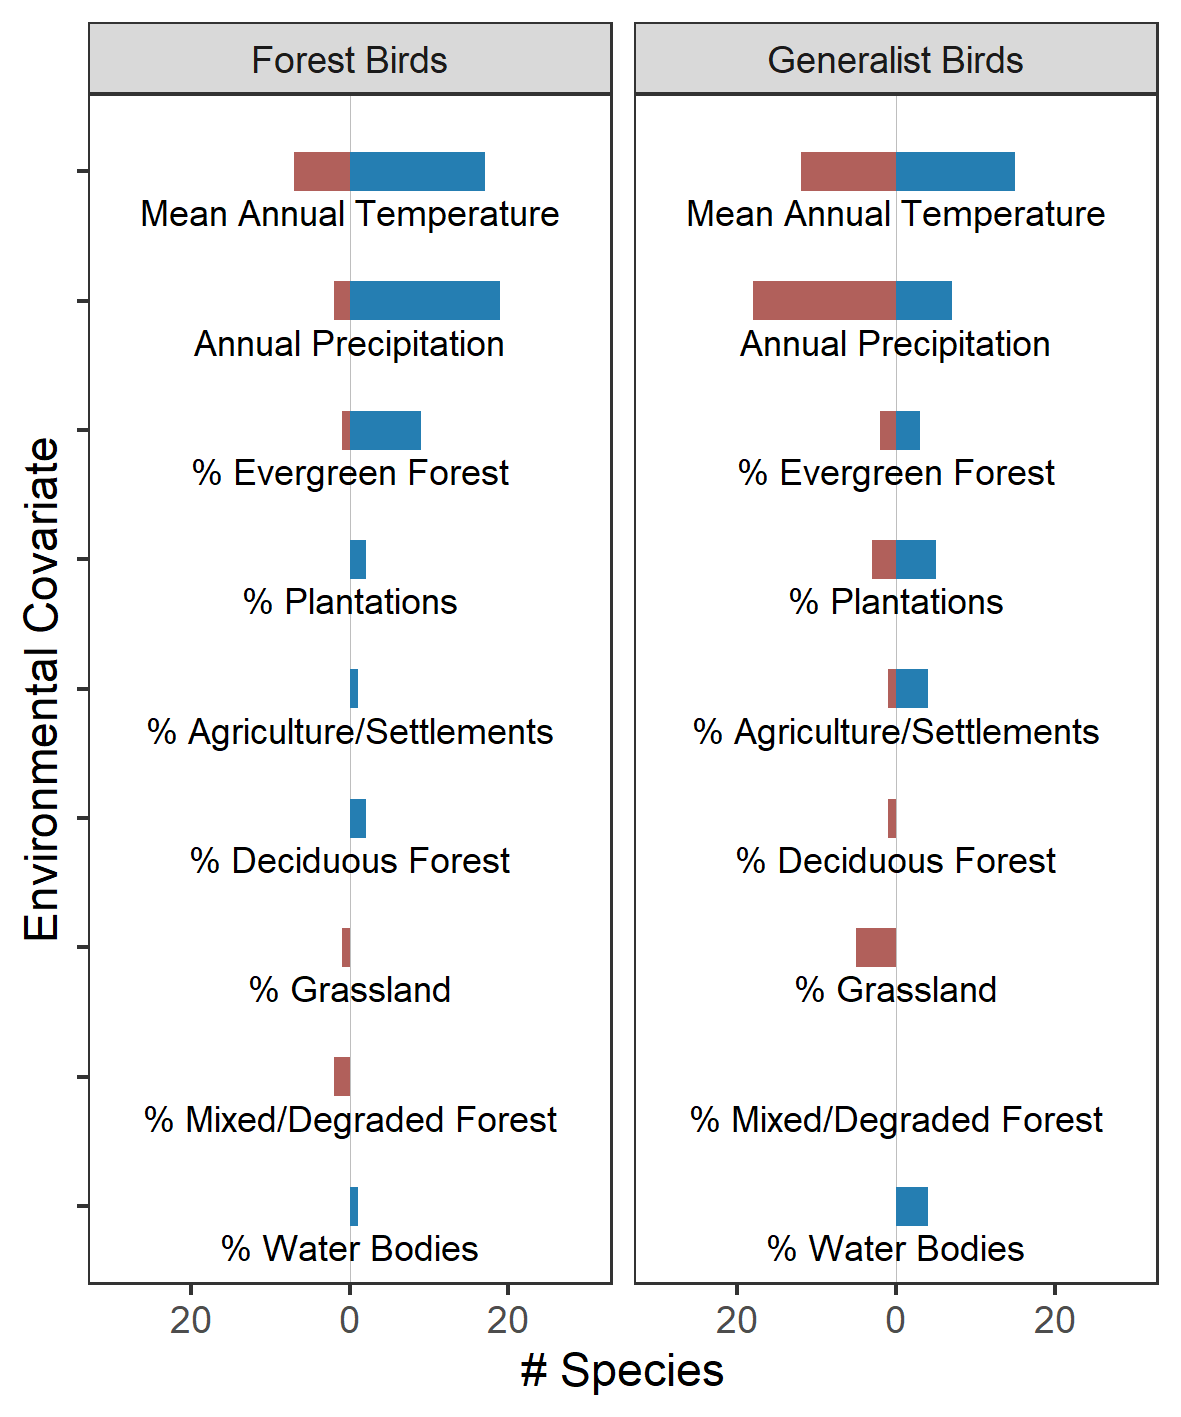
\includegraphics{figs/fig_04.png}
\caption{\textbf{Environmental predictors and species-specific associations}
The direction of association between species-specific probability of occupancy and climatic and landscape predictors is shown here (as a function of habitat preference). Blue colors show the number of species that are positively associated with a climatic/landscape predictor while red colors show the number of species that are negatively associated with a climatic/landscape predictor (see Table 1 for the number of forest/generalist species that show positive/negative association with each of the predictors).}
\end{figure}

\hypertarget{predicting-species-specific-occupancy-as-a-function-of-significant-predictors}{%
\section{Predicting species-specific occupancy as a function of significant predictors}\label{predicting-species-specific-occupancy-as-a-function-of-significant-predictors}}

This script plots species-specific probabilities of occupancy as a function of significant environmental predictors and maps occupancy across the study area for a given list of species and significant predictors.

\hypertarget{prepare-libraries-5}{%
\subsection{Prepare libraries}\label{prepare-libraries-5}}

\begin{Shaded}
\begin{Highlighting}[]
\CommentTok{# to handle data}
\KeywordTok{library}\NormalTok{(dplyr)}
\KeywordTok{library}\NormalTok{(readr)}
\KeywordTok{library}\NormalTok{(tidyr)}
\KeywordTok{library}\NormalTok{(purrr)}
\KeywordTok{library}\NormalTok{(stringr)}
\KeywordTok{library}\NormalTok{(glue)}
\CommentTok{# library(data.table)}

\CommentTok{# plotting}
\KeywordTok{library}\NormalTok{(ggplot2)}
\KeywordTok{library}\NormalTok{(patchwork)}
\end{Highlighting}
\end{Shaded}

\hypertarget{read-data}{%
\subsection{Read data}\label{read-data}}

\begin{Shaded}
\begin{Highlighting}[]
\CommentTok{# read coefficient effect data}
\NormalTok{data <-}\StringTok{ }\KeywordTok{read_csv}\NormalTok{(}\StringTok{"data/results/data_predictor_effect.csv"}\NormalTok{)}

\CommentTok{# check for a predictor column}
\NormalTok{assertthat}\OperatorTok{::}\KeywordTok{assert_that}\NormalTok{(}
  \KeywordTok{all}\NormalTok{(}\KeywordTok{c}\NormalTok{(}\StringTok{"predictor"}\NormalTok{, }\StringTok{"coefficient"}\NormalTok{, }\StringTok{"se"}\NormalTok{) }\OperatorTok\StringTok{ }\KeywordTok{colnames}\NormalTok{(data)),}
  \DataTypeTok{msg =} \StringTok{"make_response_data: data must have columns called 'predictor',}
\StringTok{    'coefficient', and 'se'"}
\NormalTok{)}
\end{Highlighting}
\end{Shaded}

\hypertarget{prepare-predictor-data}{%
\subsection{Prepare predictor data}\label{prepare-predictor-data}}

\begin{Shaded}
\begin{Highlighting}[]
\CommentTok{# preparep predictors - now look only for any digits}
\NormalTok{predictors <-}\StringTok{ }\KeywordTok{c}\NormalTok{(}\StringTok{"bio}\CharTok{\textbackslash{}\textbackslash{}}\StringTok{d+"}\NormalTok{, }\KeywordTok{glue}\NormalTok{(}\StringTok{"lc_0\{seq(9)\}"}\NormalTok{))}

\CommentTok{# prepare predictor search strings and scaling power}
\NormalTok{preds <-}\StringTok{ }\KeywordTok{glue}\NormalTok{(}\StringTok{"(\{predictors\})"}\NormalTok{)}
\NormalTok{preds <-}\StringTok{ }\KeywordTok{str_flatten}\NormalTok{(preds, }\DataTypeTok{collapse =} \StringTok{"|"}\NormalTok{)}

\CommentTok{# some way of identifying square terms}
\NormalTok{power <-}\StringTok{ }\NormalTok{(}\KeywordTok{str_extract}\NormalTok{(data}\OperatorTok{$}\NormalTok{predictor, }\StringTok{"Ibio"}\NormalTok{))}
\NormalTok{power[}\OperatorTok{!}\KeywordTok{is.na}\NormalTok{(power)] =}\StringTok{ }\DecValTok{2}
\NormalTok{power[}\KeywordTok{is.na}\NormalTok{(power)] <-}\StringTok{ }\DecValTok{1}
\NormalTok{power =}\StringTok{ }\KeywordTok{as.numeric}\NormalTok{(power)}

\CommentTok{# assign predictor name and power}
\NormalTok{data <-}
\StringTok{  }\KeywordTok{mutate}\NormalTok{(}
\NormalTok{  data,}
  \DataTypeTok{predictor =} \KeywordTok{str_extract}\NormalTok{(predictor, preds),}
  \DataTypeTok{power =}\NormalTok{ power}
\NormalTok{)}
\end{Highlighting}
\end{Shaded}

\hypertarget{get-predictor-responses}{%
\subsection{Get predictor responses}\label{get-predictor-responses}}

\begin{Shaded}
\begin{Highlighting}[]
\CommentTok{# make predictor sequences}
\NormalTok{data <-}\StringTok{ }\KeywordTok{mutate}\NormalTok{(}
\NormalTok{  data,}
  \DataTypeTok{pred_val =} \KeywordTok{map}\NormalTok{(}
\NormalTok{    predictor,}
    \ControlFlowTok{function}\NormalTok{(x) \{}
      \KeywordTok{seq}\NormalTok{(}\DecValTok{0}\NormalTok{, }\DecValTok{1}\NormalTok{, }\FloatTok{0.05}\NormalTok{)}
\NormalTok{    \}}
\NormalTok{  ),}
  \CommentTok{#handle squared terms}
  \DataTypeTok{pred_val_pow =}\NormalTok{ purrr}\OperatorTok{::}\KeywordTok{map2}\NormalTok{(}
\NormalTok{    pred_val, power,}
    \ControlFlowTok{function}\NormalTok{(x, y) \{}
\NormalTok{      x}\OperatorTok{^}\NormalTok{y}
\NormalTok{    \}}
\NormalTok{))}


\CommentTok{# get coefficient and error times terms}
\NormalTok{data_resp <-}\StringTok{ }\KeywordTok{mutate}\NormalTok{(}
\NormalTok{  data,}
  \DataTypeTok{response =} \KeywordTok{map2}\NormalTok{(}
\NormalTok{    pred_val_pow, coefficient,}
    \ControlFlowTok{function}\NormalTok{(x, y) \{}
\NormalTok{      x }\OperatorTok{*}\StringTok{ }\NormalTok{y}
\NormalTok{    \}}
\NormalTok{  ),}
  \DataTypeTok{resp_var =} \KeywordTok{map2}\NormalTok{(}
\NormalTok{    pred_val_pow, se,}
    \ControlFlowTok{function}\NormalTok{(x, y) \{}
\NormalTok{      x }\OperatorTok{*}\StringTok{ }\NormalTok{y}
\NormalTok{    \}}
\NormalTok{  )}
\NormalTok{)}
\end{Highlighting}
\end{Shaded}

\hypertarget{get-probability-of-occupancy}{%
\subsection{Get probability of occupancy}\label{get-probability-of-occupancy}}

\begin{Shaded}
\begin{Highlighting}[]
\CommentTok{# unnest and get responses}
\NormalTok{data_resp <-}\StringTok{ }\KeywordTok{unnest}\NormalTok{(}
\NormalTok{  data_resp,}
  \DataTypeTok{cols =} \KeywordTok{c}\NormalTok{(}\StringTok{"response"}\NormalTok{, }\StringTok{"resp_var"}\NormalTok{, }\StringTok{"pred_val"}\NormalTok{)}
\NormalTok{)}

\CommentTok{# get responses for quadratic terms}
\NormalTok{data_resp <-}
\StringTok{  }\KeywordTok{group_by}\NormalTok{(}
\NormalTok{    data_resp,}
\NormalTok{    scientific_name, predictor, pred_val}
\NormalTok{  ) }\OperatorTok
\StringTok{  }\NormalTok{dplyr}\OperatorTok{::}\KeywordTok{select}\NormalTok{(}\OperatorTok{-}\NormalTok{power, }\OperatorTok{-}\NormalTok{coefficient, }\OperatorTok{-}\NormalTok{se) }\OperatorTok
\StringTok{  }\KeywordTok{summarise}\NormalTok{(}
    \KeywordTok{across}\NormalTok{(}
      \DataTypeTok{.cols =} \KeywordTok{c}\NormalTok{(}\StringTok{"response"}\NormalTok{, }\StringTok{"resp_var"}\NormalTok{),}
      \DataTypeTok{.fns =}\NormalTok{ sum}
\NormalTok{    ),}
    \DataTypeTok{.groups =} \StringTok{"keep"}
\NormalTok{  )}

\CommentTok{# get probability of occupancy}
\NormalTok{data_resp <-}\StringTok{ }\KeywordTok{ungroup}\NormalTok{(}
\NormalTok{  data_resp}
\NormalTok{) }\OperatorTok
\StringTok{  }\KeywordTok{mutate}\NormalTok{(}
    \DataTypeTok{p_occu =} \DecValTok{1} \OperatorTok{/}\StringTok{ }\NormalTok{(}\DecValTok{1} \OperatorTok{+}\StringTok{ }\KeywordTok{exp}\NormalTok{(}\OperatorTok{-}\NormalTok{response)),}
    \DataTypeTok{p_occu_low =} \DecValTok{1} \OperatorTok{/}\StringTok{ }\NormalTok{(}\DecValTok{1} \OperatorTok{+}\StringTok{ }\KeywordTok{exp}\NormalTok{(}\OperatorTok{-}\NormalTok{(response }\OperatorTok{-}\StringTok{ }\NormalTok{resp_var))),}
    \DataTypeTok{p_occu_high =} \DecValTok{1} \OperatorTok{/}\StringTok{ }\NormalTok{(}\DecValTok{1} \OperatorTok{+}\StringTok{ }\KeywordTok{exp}\NormalTok{(}\OperatorTok{-}\NormalTok{(response }\OperatorTok{+}\StringTok{ }\NormalTok{resp_var)))}
\NormalTok{  )}
\end{Highlighting}
\end{Shaded}

\hypertarget{add-scaling-for-predictors}{%
\subsection{Add scaling for predictors}\label{add-scaling-for-predictors}}

\begin{Shaded}
\begin{Highlighting}[]
\CommentTok{# scale predictors}
\NormalTok{scale15 <-}\StringTok{ }\KeywordTok{c}\NormalTok{(}\DecValTok{30}\NormalTok{, }\DecValTok{50}\NormalTok{) }\CommentTok{# range of precpitation}
\NormalTok{scale4 <-}\StringTok{ }\KeywordTok{c}\NormalTok{(}\DecValTok{0}\NormalTok{, }\DecValTok{1}\NormalTok{) }\CommentTok{# range of temperatures}

\CommentTok{# scale bio4a and bio15a by actual values}
\NormalTok{data_resp <-}\StringTok{ }\KeywordTok{mutate}\NormalTok{(}
\NormalTok{  data_resp,}
  \DataTypeTok{pred_val =} \KeywordTok{case_when}\NormalTok{(}
\NormalTok{    predictor }\OperatorTok{==}\StringTok{ "bio4"} \OperatorTok{~}\StringTok{ }\NormalTok{scales}\OperatorTok{::}\KeywordTok{rescale}\NormalTok{(pred_val, }\DataTypeTok{to =}\NormalTok{ scale4),}
\NormalTok{    predictor }\OperatorTok{==}\StringTok{ "bio15"} \OperatorTok{~}\StringTok{ }\NormalTok{scales}\OperatorTok{::}\KeywordTok{rescale}\NormalTok{(pred_val, }\DataTypeTok{to =}\NormalTok{ scale15),}
\NormalTok{    T }\OperatorTok{~}\StringTok{ }\NormalTok{pred_val}
\NormalTok{  )}
\NormalTok{)}

\CommentTok{# make long}
\NormalTok{data_poccu <-}\StringTok{ }\NormalTok{dplyr}\OperatorTok{::}\KeywordTok{select}\NormalTok{(}
\NormalTok{  data_resp,}
  \OperatorTok{-}\NormalTok{response, }\OperatorTok{-}\NormalTok{resp_var}
\NormalTok{)}
\end{Highlighting}
\end{Shaded}

\begin{Shaded}
\begin{Highlighting}[]
\CommentTok{# select species}
\NormalTok{soi <-}\StringTok{ }\KeywordTok{c}\NormalTok{(}
  \StringTok{"Myophonus horsfieldii"}\NormalTok{, }\StringTok{"Merops leschenaulti"}\NormalTok{,}
  \StringTok{"Acrocephalus dumetorum"}\NormalTok{, }\StringTok{"Pycnonotus cafer"}
\NormalTok{)}
\NormalTok{which_predictors <-}\StringTok{ }\KeywordTok{c}\NormalTok{(}\StringTok{"bio4"}\NormalTok{)}
\end{Highlighting}
\end{Shaded}

\hypertarget{figure-occupancy-predictors}{%
\subsubsection{Figure: Occupancy \textasciitilde{} predictors}\label{figure-occupancy-predictors}}

\begin{Shaded}
\begin{Highlighting}[]
\NormalTok{data_fig <-}\StringTok{ }\NormalTok{data_poccu }\OperatorTok
\StringTok{  }\KeywordTok{filter}\NormalTok{(}
\NormalTok{    scientific_name }\OperatorTok\StringTok{ }\NormalTok{soi,}
\NormalTok{    predictor }\OperatorTok\StringTok{ }\NormalTok{which_predictors}
\NormalTok{  ) }\OperatorTok
\StringTok{  }\KeywordTok{mutate}\NormalTok{(}
    \DataTypeTok{cat =} \KeywordTok{case_when}\NormalTok{(}
\NormalTok{      scientific_name }\OperatorTok\StringTok{ }\KeywordTok{c}\NormalTok{(}\StringTok{"Myophonus horsfieldii"}\NormalTok{, }\StringTok{"Merops leschenaulti"}\NormalTok{) }\OperatorTok{~}\StringTok{ "forest"}\NormalTok{,}
\NormalTok{      T }\OperatorTok{~}\StringTok{ "general"}
\NormalTok{    )}
\NormalTok{  )}

\CommentTok{# split data}
\NormalTok{data_fig <-}\StringTok{ }\KeywordTok{nest}\NormalTok{(}
\NormalTok{  data_fig,}
  \OperatorTok{-}\NormalTok{cat}
\NormalTok{)}
\end{Highlighting}
\end{Shaded}

\begin{Shaded}
\begin{Highlighting}[]
\CommentTok{# make plots}
\NormalTok{make_occu_fig <-}\StringTok{ }\ControlFlowTok{function}\NormalTok{(df, this_fill) \{}
  \KeywordTok{ggplot}\NormalTok{(}
\NormalTok{    df}
\NormalTok{  ) }\OperatorTok{+}
\StringTok{    }\KeywordTok{geom_ribbon}\NormalTok{(}
      \KeywordTok{aes}\NormalTok{(}
\NormalTok{        pred_val,}
        \DataTypeTok{ymin =}\NormalTok{ p_occu_low,}
        \DataTypeTok{ymax =}\NormalTok{ p_occu_high}
\NormalTok{      ),}
      \DataTypeTok{fill =}\NormalTok{ this_fill,}
      \DataTypeTok{alpha =} \FloatTok{0.5}
\NormalTok{    ) }\OperatorTok{+}
\StringTok{    }\KeywordTok{geom_line}\NormalTok{(}
      \KeywordTok{aes}\NormalTok{(}
\NormalTok{        pred_val, p_occu}
\NormalTok{      ),}
      \DataTypeTok{size =} \DecValTok{1}
\NormalTok{    ) }\OperatorTok{+}
\StringTok{    }\KeywordTok{facet_grid}\NormalTok{(}
      \OperatorTok{~}\NormalTok{scientific_name}
\NormalTok{    ) }\OperatorTok{+}
\StringTok{    }\KeywordTok{theme_test}\NormalTok{(}
      \DataTypeTok{base_family =} \StringTok{"Arial"}
\NormalTok{    ) }\OperatorTok{+}
\StringTok{    }\KeywordTok{theme}\NormalTok{(}
      \DataTypeTok{strip.text =} \KeywordTok{element_text}\NormalTok{(}
        \DataTypeTok{face =} \StringTok{"italic"}
\NormalTok{      )}
\NormalTok{    ) }\OperatorTok{+}
\StringTok{    }\KeywordTok{labs}\NormalTok{(}
      \DataTypeTok{x =} \StringTok{"Temperature seasonality"}\NormalTok{,}
      \DataTypeTok{y =} \StringTok{"Probability of occupancy"}
\NormalTok{    )}
\NormalTok{\}}


\NormalTok{fig_occu <-}\StringTok{ }\KeywordTok{map2}\NormalTok{(data_fig}\OperatorTok{$}\NormalTok{data, }\StringTok{"grey"}\NormalTok{, make_occu_fig)}

\NormalTok{fig_occu <-}
\StringTok{  }\KeywordTok{wrap_plots}\NormalTok{(}
\NormalTok{    fig_occu[}\KeywordTok{c}\NormalTok{(}\DecValTok{2}\NormalTok{, }\DecValTok{1}\NormalTok{)],}
    \DataTypeTok{ncol =} \DecValTok{1}
\NormalTok{  ) }\OperatorTok{&}\StringTok{ }\KeywordTok{plot_annotation}\NormalTok{(}
    \DataTypeTok{tag_levels =} \StringTok{"a"}
\NormalTok{  ) }\OperatorTok{&}
\StringTok{    }\KeywordTok{theme}\NormalTok{(}
      \DataTypeTok{plot.tag =} \KeywordTok{element_text}\NormalTok{(}
        \DataTypeTok{face =} \StringTok{"bold"}
\NormalTok{      )}
\NormalTok{    )}

\CommentTok{# save figure}
\KeywordTok{ggsave}\NormalTok{(}
\NormalTok{  fig_occu,}
  \DataTypeTok{filename =} \StringTok{"figs/fig_05.png"}\NormalTok{,}
  \DataTypeTok{width =} \DecValTok{5}\NormalTok{, }\DataTypeTok{height =} \FloatTok{5.5}
\NormalTok{)}
\end{Highlighting}
\end{Shaded}

\begin{figure}
\centering
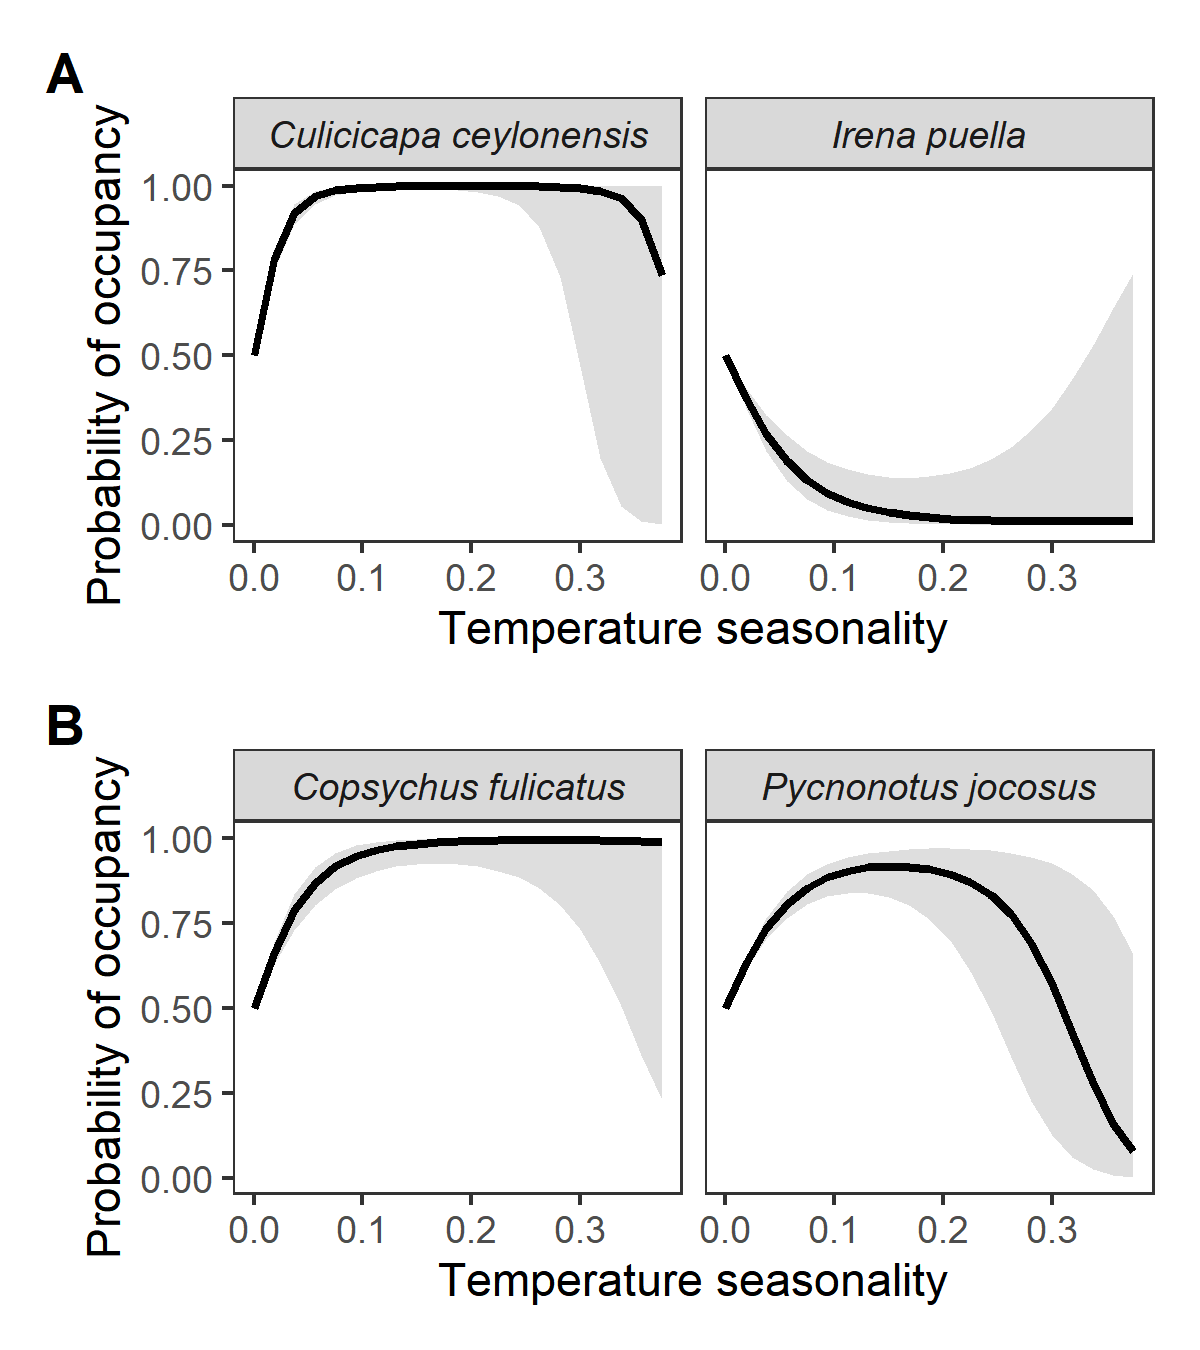
\includegraphics{figs/fig_05.png}
\caption{\textbf{Probability of occupancy as a function of temperature seasonality.}
Predicted probability of occupancy curves as a function of temperature seasonality for two (a) generalist and (b) forest species are shown here. (a) Temperature seasonality is negatively associated with the probability of occupancy of the chestnut-headed bee-eater \emph{Merops leschenaulti} and the Malabar whistling-thrush \emph{Myophonus horsfieldii}. (b) Temperature seasonality is positively associated with the probability of occupancy of the Blyth's reed warbler \emph{Acrocephalus dumetorum} and the red-vented bulbul \emph{Pycnonotus cafer}.}
\end{figure}

\hypertarget{figures-occupancy-predictors-for-all-species}{%
\subsubsection{Figures: Occupancy \textasciitilde{} predictors for all species}\label{figures-occupancy-predictors-for-all-species}}

\begin{Shaded}
\begin{Highlighting}[]
\NormalTok{data_fig <-}\StringTok{ }\KeywordTok{nest}\NormalTok{(}
\NormalTok{  data_poccu,}
  \OperatorTok{-}\NormalTok{scientific_name, }\OperatorTok{-}\NormalTok{predictor}
\NormalTok{)}

\NormalTok{pred_names <-}\StringTok{ }\KeywordTok{c}\NormalTok{(}
  \StringTok{"bio4"}\NormalTok{ =}\StringTok{ "Temp. seasonality"}\NormalTok{,}
  \StringTok{"bio15"}\NormalTok{ =}\StringTok{ "Precip. seasonality"}\NormalTok{,}
  \StringTok{"lc_01"}\NormalTok{ =}\StringTok{ "Evergreen"}\NormalTok{,}
  \StringTok{"lc_02"}\NormalTok{ =}\StringTok{ "Deciduous"}\NormalTok{,}
  \StringTok{"lc_03"}\NormalTok{ =}\StringTok{ "Mixed/degraded"}\NormalTok{,}
  \StringTok{"lc_04"}\NormalTok{ =}\StringTok{ "Agri./Settl."}\NormalTok{,}
  \StringTok{"lc_05"}\NormalTok{ =}\StringTok{ "Grassland"}\NormalTok{,}
  \StringTok{"lc_07"}\NormalTok{ =}\StringTok{ "Plantation"}\NormalTok{,}
  \StringTok{"lc_09"}\NormalTok{ =}\StringTok{ "Water"}
\NormalTok{)}

\NormalTok{pred_names <-}\StringTok{ }\KeywordTok{tibble}\NormalTok{(}
  \DataTypeTok{name =}\NormalTok{ pred_names,}
  \DataTypeTok{predictor =} \KeywordTok{names}\NormalTok{(pred_names)}
\NormalTok{)}

\NormalTok{data_fig <-}\StringTok{ }\KeywordTok{left_join}\NormalTok{(}
\NormalTok{  data_fig,}
\NormalTok{  pred_names}
\NormalTok{)}

\NormalTok{data_fig <-}\StringTok{ }\KeywordTok{mutate}\NormalTok{(}
\NormalTok{  data_fig,}
  \DataTypeTok{plots =} \KeywordTok{map}\NormalTok{(}
\NormalTok{    data, }\ControlFlowTok{function}\NormalTok{(df) \{}
      \KeywordTok{ggplot}\NormalTok{(df) }\OperatorTok{+}
\StringTok{        }\KeywordTok{geom_ribbon}\NormalTok{(}
          \KeywordTok{aes}\NormalTok{(}
\NormalTok{            pred_val,}
            \DataTypeTok{ymin =}\NormalTok{ p_occu_low,}
            \DataTypeTok{ymax =}\NormalTok{ p_occu_high}
\NormalTok{          ),}
          \DataTypeTok{fill =} \StringTok{"grey"}\NormalTok{,}
          \DataTypeTok{alpha =} \FloatTok{0.5}
\NormalTok{        ) }\OperatorTok{+}
\StringTok{        }\KeywordTok{geom_line}\NormalTok{(}
          \KeywordTok{aes}\NormalTok{(}
\NormalTok{            pred_val, p_occu}
\NormalTok{          )}
\NormalTok{        ) }\OperatorTok{+}
\StringTok{        }\KeywordTok{coord_cartesian}\NormalTok{(}
          \DataTypeTok{ylim =} \KeywordTok{c}\NormalTok{(}\DecValTok{0}\NormalTok{, }\DecValTok{1}\NormalTok{)}
\NormalTok{        ) }\OperatorTok{+}
\StringTok{        }\KeywordTok{theme_test}\NormalTok{(}
          \DataTypeTok{base_family =} \StringTok{"Arial"}
\NormalTok{        ) }\OperatorTok{+}
\StringTok{        }\KeywordTok{labs}\NormalTok{(}
          \DataTypeTok{x =} \StringTok{"Predictor"}\NormalTok{,}
          \DataTypeTok{y =} \StringTok{"p(Occupancy)"}
\NormalTok{        )}
\NormalTok{    \}}
\NormalTok{  )}
\NormalTok{)}

\CommentTok{# add names}
\NormalTok{data_fig <-}\StringTok{ }\KeywordTok{mutate}\NormalTok{(}
\NormalTok{  data_fig,}
  \DataTypeTok{plots =} \KeywordTok{map2}\NormalTok{(}
\NormalTok{    plots, name,}
    \ControlFlowTok{function}\NormalTok{(p, name) \{}
\NormalTok{      p <-}\StringTok{ }\NormalTok{p }\OperatorTok{+}\StringTok{ }\KeywordTok{labs}\NormalTok{(}
        \DataTypeTok{x =}\NormalTok{ name}
\NormalTok{      )}
\NormalTok{    \}}
\NormalTok{  )}
\NormalTok{)}

\CommentTok{# summarise as patchwork}
\NormalTok{data_fig <-}\StringTok{ }\KeywordTok{group_by}\NormalTok{(}
\NormalTok{  data_fig,}
\NormalTok{  scientific_name}
\NormalTok{) }\OperatorTok
\StringTok{  }\KeywordTok{summarise}\NormalTok{(}
    \DataTypeTok{plots =} \KeywordTok{list}\NormalTok{(}
      \KeywordTok{wrap_plots}\NormalTok{(}
\NormalTok{        plots,}
        \DataTypeTok{ncol =} \DecValTok{5}
\NormalTok{      )}
\NormalTok{    )}
\NormalTok{  )}

\CommentTok{# add title as sp}
\NormalTok{data_fig <-}\StringTok{ }\KeywordTok{mutate}\NormalTok{(}
\NormalTok{  data_fig,}
  \DataTypeTok{plots =} \KeywordTok{map2}\NormalTok{(}
\NormalTok{    plots, scientific_name,}
    \ControlFlowTok{function}\NormalTok{(p, name) \{}
\NormalTok{      p <-}\StringTok{ }\NormalTok{p }\OperatorTok{&}\StringTok{ }\KeywordTok{plot_annotation}\NormalTok{(}
        \DataTypeTok{title =}\NormalTok{ name}
\NormalTok{      )}
\NormalTok{    \}}
\NormalTok{  )}
\NormalTok{)}
\end{Highlighting}
\end{Shaded}

\begin{Shaded}
\begin{Highlighting}[]
\CommentTok{# save images}
\KeywordTok{cairo_pdf}\NormalTok{(}
  \DataTypeTok{filename =} \StringTok{"figs/fig_occupancy_predictors.pdf"}\NormalTok{,}
  \DataTypeTok{onefile =} \OtherTok{TRUE}\NormalTok{, }\DataTypeTok{width =} \DecValTok{10}\NormalTok{, }\DataTypeTok{height =} \DecValTok{2}
\NormalTok{)}
\NormalTok{data_fig}\OperatorTok{$}\NormalTok{plots}
\KeywordTok{dev.off}\NormalTok{()}
\end{Highlighting}
\end{Shaded}

\hypertarget{mapping-species-occupancy}{%
\subsection{Mapping species occupancy}\label{mapping-species-occupancy}}

\hypertarget{read-in-raster-layers}{%
\subsubsection{Read in raster layers}\label{read-in-raster-layers}}

\begin{Shaded}
\begin{Highlighting}[]
\KeywordTok{library}\NormalTok{(terra)}
\KeywordTok{library}\NormalTok{(sf)}
\end{Highlighting}
\end{Shaded}

\begin{Shaded}
\begin{Highlighting}[]
\CommentTok{# read saved rasters}
\NormalTok{lscape =}\StringTok{ }\KeywordTok{rast}\NormalTok{(}\StringTok{"data/spatial/landscape_resamp01_km.tif"}\NormalTok{)}

\CommentTok{# isolate temperature and rainfall}
\NormalTok{bio4 =}\StringTok{ }\NormalTok{lscape[[}\DecValTok{4}\NormalTok{]] }
\NormalTok{bio15 =}\StringTok{ }\NormalTok{lscape[[}\DecValTok{5}\NormalTok{]] }\CommentTok{# rain}

\CommentTok{# careful while loading this raster, large size}
\NormalTok{landcover <-}\StringTok{ }\KeywordTok{rast}\NormalTok{(}\StringTok{"data/landUseClassification/landcover_roy_2015_reclassified.tif"}\NormalTok{)}

\NormalTok{lc_1km <-}\StringTok{ }\KeywordTok{rast}\NormalTok{(}\StringTok{"data/landUseClassification/lc_01000m.tif"}\NormalTok{)}
\end{Highlighting}
\end{Shaded}

\hypertarget{split-landcover-into-proportions-per-1km}{%
\subsubsection{Split landcover into proportions per 1km}\label{split-landcover-into-proportions-per-1km}}

\begin{Shaded}
\begin{Highlighting}[]
\CommentTok{# separate the fine-scale landcover raster into presence-absence of each class}
\NormalTok{lc_split <-}\StringTok{ }\KeywordTok{segregate}\NormalTok{(landcover)}

\CommentTok{# resample to 1km}
\CommentTok{# bilinear resampling uses the mean function.}
\CommentTok{# mean of N 0s and 1s is the proportion of 1s, ie, proportion of each landcover}
\NormalTok{lc_split <-}\StringTok{ }\NormalTok{terra}\OperatorTok{::}\KeywordTok{resample}\NormalTok{(}
\NormalTok{  lc_split,}
\NormalTok{  lc_1km,}
  \DataTypeTok{method =} \StringTok{"bilinear"}
\NormalTok{)}

\CommentTok{# rename rasters}
\KeywordTok{names}\NormalTok{(lc_split) <-}\StringTok{ }\NormalTok{pred_names}\OperatorTok{$}\NormalTok{name[}\OperatorTok{-}\KeywordTok{c}\NormalTok{(}\DecValTok{1}\NormalTok{, }\DecValTok{2}\NormalTok{)]}

\CommentTok{# save raster of landcover proportion}
\NormalTok{terra}\OperatorTok{::}\KeywordTok{writeRaster}\NormalTok{(}
\NormalTok{  lc_split,}
  \DataTypeTok{filename =} \StringTok{"data/spatial/raster_landcover_proportion_1km.tif"}\NormalTok{,}
  \DataTypeTok{overwrite=}\OtherTok{TRUE}
\NormalTok{)}

\KeywordTok{rm}\NormalTok{(landcover)}
\KeywordTok{gc}\NormalTok{()}
\end{Highlighting}
\end{Shaded}

\begin{Shaded}
\begin{Highlighting}[]
\CommentTok{# plot proportion of landcover classes}
\KeywordTok{png}\NormalTok{(}\DataTypeTok{width =} \DecValTok{1200} \OperatorTok{*}\StringTok{ }\DecValTok{2}\NormalTok{, }\DataTypeTok{height =} \DecValTok{1200} \OperatorTok{*}\StringTok{ }\DecValTok{2}\NormalTok{, }\DataTypeTok{filename =} \StringTok{"figs/fig_landcover_proportion_1km.png"}\NormalTok{, }\DataTypeTok{res =} \DecValTok{300}\NormalTok{)}
\KeywordTok{plot}\NormalTok{(}
\NormalTok{  lc_split,}
  \DataTypeTok{col =}\NormalTok{ colorspace}\OperatorTok{::}\KeywordTok{sequential_hcl}\NormalTok{(}\DecValTok{20}\NormalTok{, }\DataTypeTok{palette =} \StringTok{"Viridis"}\NormalTok{),}
  \DataTypeTok{range =} \KeywordTok{c}\NormalTok{(}\DecValTok{0}\NormalTok{, }\DecValTok{1}\NormalTok{)}
\NormalTok{)}
\KeywordTok{dev.off}\NormalTok{()}
\end{Highlighting}
\end{Shaded}

\hypertarget{prepare-climatic-layers}{%
\subsubsection{Prepare climatic layers}\label{prepare-climatic-layers}}

\begin{Shaded}
\begin{Highlighting}[]
\CommentTok{# load landcover split}
\NormalTok{lc_split =}\StringTok{ }\NormalTok{terra}\OperatorTok{::}\KeywordTok{rast}\NormalTok{(}\StringTok{"data/spatial/raster_landcover_proportion_1km.tif"}\NormalTok{)}
\end{Highlighting}
\end{Shaded}

\hypertarget{mask-by-study-area}{%
\subsubsection{Mask by study area}\label{mask-by-study-area}}

\begin{Shaded}
\begin{Highlighting}[]
\CommentTok{# mask by hills}
\CommentTok{# run only if required (makes more sense to map to a larger area)}
\NormalTok{hills =}\StringTok{ }\KeywordTok{st_read}\NormalTok{(}\StringTok{"data/spatial/hillsShapefile/Nil_Ana_Pal.shp"}\NormalTok{) }\OperatorTok\StringTok{ }
\StringTok{  }\KeywordTok{st_transform}\NormalTok{(}\DecValTok{32643}\NormalTok{)}

\CommentTok{#bio_1 = terra::mask(}
\CommentTok{#  bio_1,}
\CommentTok{#  vect(hills)}
\CommentTok{#)}

\CommentTok{#bio_12 = terra::mask(}
\CommentTok{#  bio_12,}
\CommentTok{#  vect(hills)}
\CommentTok{#)}
\end{Highlighting}
\end{Shaded}

\begin{Shaded}
\begin{Highlighting}[]
\CommentTok{# get ranges}
\NormalTok{range4 <-}\StringTok{ }\NormalTok{terra}\OperatorTok{::}\KeywordTok{minmax}\NormalTok{(bio4)[, }\DecValTok{1}\NormalTok{] }
\NormalTok{range15 <-}\StringTok{ }\NormalTok{terra}\OperatorTok{::}\KeywordTok{minmax}\NormalTok{(bio15)[, }\DecValTok{1}\NormalTok{]}

\CommentTok{# rescale}
\NormalTok{bio4 <-}\StringTok{ }\NormalTok{(bio4 }\OperatorTok{-}\StringTok{ }\KeywordTok{min}\NormalTok{(range4)) }\OperatorTok{/}\StringTok{ }\NormalTok{(}\KeywordTok{diff}\NormalTok{(range4))}
\NormalTok{bio15 <-}\StringTok{ }\NormalTok{(bio15 }\OperatorTok{-}\StringTok{ }\KeywordTok{min}\NormalTok{(range15)) }\OperatorTok{/}\StringTok{ }\NormalTok{(}\KeywordTok{diff}\NormalTok{(range15))}

\CommentTok{# project to UTM}
\NormalTok{climate <-}\StringTok{ }\KeywordTok{c}\NormalTok{(bio4, bio15)}
\KeywordTok{names}\NormalTok{(climate) =}\StringTok{ }\KeywordTok{c}\NormalTok{(}
  \StringTok{"Temp. seasonality"}\NormalTok{, }
  \StringTok{"Precip. seasonality"}
\NormalTok{)}

\NormalTok{climate <-}\StringTok{ }\NormalTok{terra}\OperatorTok{::}\KeywordTok{project}\NormalTok{(}
  \DataTypeTok{x =}\NormalTok{ climate, }\DataTypeTok{y =}\NormalTok{ lc_1km}
\NormalTok{)}

\CommentTok{# make squared terms}
\NormalTok{climate2 <-}\StringTok{ }\NormalTok{climate }\OperatorTok{*}\StringTok{ }\NormalTok{climate}

\CommentTok{# names}
\KeywordTok{names}\NormalTok{(climate2) =}\StringTok{ }\KeywordTok{glue}\NormalTok{(}\StringTok{"\{names(climate)\} 2"}\NormalTok{)}

\CommentTok{# add to landcover proportions and plot}
\NormalTok{landscape <-}\StringTok{ }\KeywordTok{c}\NormalTok{(climate, lc_split)}
\end{Highlighting}
\end{Shaded}

\hypertarget{plot-full-bounds-of-landscape-variables}{%
\subsubsection{Plot full bounds of landscape variables}\label{plot-full-bounds-of-landscape-variables}}

\begin{Shaded}
\begin{Highlighting}[]
\CommentTok{# plot proportion of landcover classes}
\KeywordTok{png}\NormalTok{(}
  \DataTypeTok{width =} \DecValTok{1200} \OperatorTok{*}\StringTok{ }\DecValTok{2}\NormalTok{, }\DataTypeTok{height =} \DecValTok{1200} \OperatorTok{*}\StringTok{ }\DecValTok{2}\NormalTok{, }\DataTypeTok{filename =} \StringTok{"figs/fig_landscape_1km.png"}\NormalTok{,}
  \DataTypeTok{res =} \DecValTok{300}
\NormalTok{)}
\KeywordTok{plot}\NormalTok{(}
\NormalTok{  landscape,}
  \DataTypeTok{col =}\NormalTok{ colorspace}\OperatorTok{::}\KeywordTok{sequential_hcl}\NormalTok{(}\DecValTok{20}\NormalTok{, }\DataTypeTok{palette =} \StringTok{"agSunset"}\NormalTok{, }\DataTypeTok{rev =}\NormalTok{ T),}
  \DataTypeTok{range =} \KeywordTok{c}\NormalTok{(}\DecValTok{0}\NormalTok{, }\DecValTok{1}\NormalTok{)}
\NormalTok{)}
\KeywordTok{dev.off}\NormalTok{()}
\end{Highlighting}
\end{Shaded}

\begin{Shaded}
\begin{Highlighting}[]
\CommentTok{# add squared terms}
\NormalTok{landscape <-}\StringTok{ }\KeywordTok{c}\NormalTok{(}
\NormalTok{  climate, climate2, lc_split}
\NormalTok{)}

\CommentTok{#landscape = terra::mask(}
\CommentTok{#  landscape,}
\CommentTok{#  vect(hills)}
\CommentTok{#)}
\end{Highlighting}
\end{Shaded}

\hypertarget{prepare-soi-predictors}{%
\subsubsection{Prepare soi predictors}\label{prepare-soi-predictors}}

Prepare the soi predictor coefficients as a vector of the same length as the number of raster layers.
These will be multiplied with each layer to give the effect of each layer.

\begin{Shaded}
\begin{Highlighting}[]
\CommentTok{# get soi coefs}
\NormalTok{sp_coefs <-}\StringTok{ }\KeywordTok{filter}\NormalTok{(}
\NormalTok{  data}
\NormalTok{) }\OperatorTok
\StringTok{  }\NormalTok{dplyr}\OperatorTok{::}\KeywordTok{select}\NormalTok{(}
    \OperatorTok{-}\NormalTok{pred_val, }\OperatorTok{-}\NormalTok{pred_val_pow}
\NormalTok{  )}

\CommentTok{# add missing landcover classes}
\NormalTok{sp_preds <-}\StringTok{ }\KeywordTok{crossing}\NormalTok{(}
  \DataTypeTok{scientific_name =}\NormalTok{ soi,}
  \DataTypeTok{predictor =}\NormalTok{ pred_names}\OperatorTok{$}\NormalTok{predictor,}
  \DataTypeTok{power =} \KeywordTok{c}\NormalTok{(}\DecValTok{1}\NormalTok{, }\DecValTok{2}\NormalTok{)}
\NormalTok{)}

\CommentTok{# remove squared terms for landcover}
\NormalTok{sp_preds <-}\StringTok{ }\KeywordTok{filter}\NormalTok{(}
\NormalTok{  sp_preds,}
  \OperatorTok{!}\NormalTok{(}\KeywordTok{str_detect}\NormalTok{(predictor, }\StringTok{"lc"}\NormalTok{) }\OperatorTok{&}\StringTok{ }\NormalTok{power }\OperatorTok{==}\StringTok{ }\DecValTok{2}\NormalTok{)}
\NormalTok{)}

\CommentTok{# correct square LC terms}
\NormalTok{sp_coefs =}\StringTok{ }\KeywordTok{mutate}\NormalTok{(}
\NormalTok{  sp_coefs,}
  \DataTypeTok{power =} \KeywordTok{if_else}\NormalTok{(}
    \KeywordTok{str_detect}\NormalTok{(predictor, }\StringTok{"lc"}\NormalTok{),}
    \DecValTok{1}\NormalTok{,}
\NormalTok{    power}
\NormalTok{  )}
\NormalTok{)}

\NormalTok{sp_coefs <-}\StringTok{ }\KeywordTok{full_join}\NormalTok{(}
\NormalTok{  sp_coefs,}
\NormalTok{  sp_preds}
\NormalTok{)}

\CommentTok{# make wide --- this should give no warnings}
\NormalTok{sp_coefs <-}
\StringTok{  }\KeywordTok{pivot_wider}\NormalTok{(}
\NormalTok{    sp_coefs,}
    \DataTypeTok{id_cols =} \KeywordTok{c}\NormalTok{(}\StringTok{"scientific_name"}\NormalTok{),}
    \DataTypeTok{names_from =} \KeywordTok{c}\NormalTok{(}\StringTok{"predictor"}\NormalTok{, }\StringTok{"power"}\NormalTok{),}
    \DataTypeTok{values_from =} \StringTok{"coefficient"}
\NormalTok{  )}

\CommentTok{# get into order}
\NormalTok{sp_coefs <-}\StringTok{ }\NormalTok{dplyr}\OperatorTok{::}\KeywordTok{select}\NormalTok{(}
\NormalTok{  sp_coefs,}
\NormalTok{  scientific_name,}
  \KeywordTok{c}\NormalTok{(}
    \StringTok{"bio4_1"}\NormalTok{, }\StringTok{"bio15_1"}\NormalTok{,}
    \StringTok{"bio4_2"}\NormalTok{, }\StringTok{"bio15_2"}
\NormalTok{  ),}
  \KeywordTok{matches}\NormalTok{(}\StringTok{"lc"}\NormalTok{)}
\NormalTok{)}

\CommentTok{# get vectors of coefficients}
\NormalTok{sp_coefs <-}\StringTok{ }\KeywordTok{nest}\NormalTok{(}
\NormalTok{  sp_coefs,}
  \OperatorTok{-}\NormalTok{scientific_name}
\NormalTok{)}
\end{Highlighting}
\end{Shaded}

\hypertarget{prepare-species-occupancy-for-soi}{%
\subsubsection{Prepare species occupancy for SOI}\label{prepare-species-occupancy-for-soi}}

Here, we shall simply multiply each landscape layer with the corresponding predictor coefficient.Where these are not available, we shall simply multiply the corresponding layer with NA. The resulting layers will be summed together to get a single response layer, which will then be inverse logit transformed to get the probability of occupancy.

\begin{Shaded}
\begin{Highlighting}[]
\CommentTok{# multiply coefficients with layers}
\NormalTok{soi_occu <-}\StringTok{ }\KeywordTok{map}\NormalTok{(}
\NormalTok{  sp_coefs[sp_coefs}\OperatorTok{$}\NormalTok{scientific_name }\OperatorTok\StringTok{ }\NormalTok{soi, ]}\OperatorTok{$}\NormalTok{data,}
  \DataTypeTok{.f =} \ControlFlowTok{function}\NormalTok{(df) \{}
\NormalTok{    response <-}\StringTok{ }\KeywordTok{unlist}\NormalTok{(}\KeywordTok{slice}\NormalTok{(df, }\DecValTok{1}\NormalTok{), }\DataTypeTok{use.names =}\NormalTok{ F) }\OperatorTok{*}\StringTok{ }\NormalTok{landscape}
\NormalTok{    response <-}\StringTok{ }\KeywordTok{sum}\NormalTok{(response, }\DataTypeTok{na.rm =} \OtherTok{TRUE}\NormalTok{) }\CommentTok{# remove NA layers, i.e., non-sig preds}

    \CommentTok{# now transform for probability occupancy}
\NormalTok{    response <-}\StringTok{ }\DecValTok{1} \OperatorTok{/}\StringTok{ }\NormalTok{(}\DecValTok{1} \OperatorTok{+}\StringTok{ }\KeywordTok{exp}\NormalTok{(}\OperatorTok{-}\NormalTok{response))}
\NormalTok{  \}}
\NormalTok{)}

\CommentTok{# assign names}
\KeywordTok{names}\NormalTok{(soi_occu) <-}\StringTok{ }\NormalTok{soi}

\CommentTok{# make single stack}
\NormalTok{soi_occu <-}\StringTok{ }\KeywordTok{reduce}\NormalTok{(soi_occu, c)}
\KeywordTok{names}\NormalTok{(soi_occu) <-}\StringTok{ }\KeywordTok{c}\NormalTok{(}\StringTok{"Myophonus horsfieldii"}\NormalTok{, }\StringTok{"Merops leschenaulti"}\NormalTok{,}\StringTok{"Acrocephalus dumetorum"}\NormalTok{,}\StringTok{"Pycnonotus cafer"}\NormalTok{)}
\end{Highlighting}
\end{Shaded}

\begin{Shaded}
\begin{Highlighting}[]
\CommentTok{# use stars for plotting with ggplot}
\KeywordTok{library}\NormalTok{(stars)}
\KeywordTok{library}\NormalTok{(colorspace)}

\NormalTok{soi_occu <-}\StringTok{ }\KeywordTok{st_as_stars}\NormalTok{(soi_occu)}

\NormalTok{fig_occu_map <-}\StringTok{ }\KeywordTok{ggplot}\NormalTok{() }\OperatorTok{+}
\StringTok{  }\KeywordTok{geom_stars}\NormalTok{(}
    \DataTypeTok{data =}\NormalTok{ soi_occu}
\NormalTok{  ) }\OperatorTok{+}
\StringTok{  }\KeywordTok{scale_fill_binned_sequential}\NormalTok{(}
    \DataTypeTok{palette =} \StringTok{"Purple-Yellow"}\NormalTok{,}
    \DataTypeTok{name =} \StringTok{"Probability of Occupancy"}\NormalTok{,}
    \DataTypeTok{rev =}\NormalTok{ T,}
    \DataTypeTok{limits =} \KeywordTok{c}\NormalTok{(}\DecValTok{0}\NormalTok{, }\DecValTok{1}\NormalTok{),}
    \DataTypeTok{breaks =} \KeywordTok{seq}\NormalTok{(}\DecValTok{0}\NormalTok{, }\DecValTok{1}\NormalTok{, }\FloatTok{0.1}\NormalTok{), }
    \DataTypeTok{na.value =} \StringTok{"grey99"}\NormalTok{,}
    \DataTypeTok{show.limits =}\NormalTok{ T}
\NormalTok{  ) }\OperatorTok{+}
\StringTok{  }\KeywordTok{facet_wrap}\NormalTok{(}
    \OperatorTok{~}\NormalTok{band,}
    \DataTypeTok{labeller =} \KeywordTok{labeller}\NormalTok{(}
      \DataTypeTok{band =} \ControlFlowTok{function}\NormalTok{(x) }\KeywordTok{str_replace}\NormalTok{(x, }\StringTok{"}\CharTok{\textbackslash{}\textbackslash{}}\StringTok{."}\NormalTok{, }\StringTok{" "}\NormalTok{)}
\NormalTok{    )}
\NormalTok{  ) }\OperatorTok{+}
\StringTok{  }\KeywordTok{coord_sf}\NormalTok{(}
    \DataTypeTok{crs =} \DecValTok{32643}\NormalTok{,}
    \DataTypeTok{expand =} \OtherTok{FALSE}
\NormalTok{  ) }\OperatorTok{+}
\StringTok{  }\KeywordTok{theme_test}\NormalTok{() }\OperatorTok{+}
\StringTok{  }\KeywordTok{theme}\NormalTok{(}
    \CommentTok{# legend.position = "rg",}
    \DataTypeTok{axis.title =} \KeywordTok{element_blank}\NormalTok{(),}
    \DataTypeTok{axis.text =} \KeywordTok{element_blank}\NormalTok{(),}
    \DataTypeTok{legend.key.height =} \KeywordTok{unit}\NormalTok{(}\DecValTok{10}\NormalTok{, }\StringTok{"mm"}\NormalTok{),}
    \DataTypeTok{legend.key.width =} \KeywordTok{unit}\NormalTok{(}\DecValTok{1}\NormalTok{, }\StringTok{"mm"}\NormalTok{),}
    \DataTypeTok{strip.text =} \KeywordTok{element_text}\NormalTok{(}
      \DataTypeTok{face =} \StringTok{"italic"}
\NormalTok{    ),}
    \DataTypeTok{legend.title =} \KeywordTok{element_text}\NormalTok{(}
      \DataTypeTok{vjust =} \DecValTok{1}
\NormalTok{    )}
\NormalTok{  )}

\CommentTok{# save figure}
\KeywordTok{ggsave}\NormalTok{(}
\NormalTok{  fig_occu_map,}
  \DataTypeTok{filename =} \StringTok{"figs/fig_06.png"}\NormalTok{,}
  \DataTypeTok{width =} \DecValTok{6}\NormalTok{, }\DataTypeTok{height =} \DecValTok{6}
\NormalTok{)}
\end{Highlighting}
\end{Shaded}

\hypertarget{prepare-species-occupancy-for-all-species}{%
\subsubsection{Prepare species occupancy for all species}\label{prepare-species-occupancy-for-all-species}}

\begin{Shaded}
\begin{Highlighting}[]
\CommentTok{# multiply coefficients with layers}
\NormalTok{sp_occu <-}\StringTok{ }\KeywordTok{map}\NormalTok{(}
\NormalTok{  sp_coefs}\OperatorTok{$}\NormalTok{data,}
  \DataTypeTok{.f =} \ControlFlowTok{function}\NormalTok{(df) \{}
\NormalTok{    response <-}\StringTok{ }\KeywordTok{unlist}\NormalTok{(}\KeywordTok{slice}\NormalTok{(df, }\DecValTok{1}\NormalTok{), }\DataTypeTok{use.names =}\NormalTok{ F) }\OperatorTok{*}\StringTok{ }\NormalTok{landscape}
\NormalTok{    response <-}\StringTok{ }\KeywordTok{sum}\NormalTok{(response, }\DataTypeTok{na.rm =} \OtherTok{TRUE}\NormalTok{) }\CommentTok{# remove NA layers, i.e., non-sig preds}

    \CommentTok{# now transform for probability occupancy}
\NormalTok{    response <-}\StringTok{ }\DecValTok{1} \OperatorTok{/}\StringTok{ }\NormalTok{(}\DecValTok{1} \OperatorTok{+}\StringTok{ }\KeywordTok{exp}\NormalTok{(}\OperatorTok{-}\NormalTok{response))}
\NormalTok{  \}}
\NormalTok{)}

\CommentTok{# make single stack}
\NormalTok{sp_occu <-}\StringTok{ }\KeywordTok{reduce}\NormalTok{(sp_occu, c)}
\CommentTok{# assign names}
\KeywordTok{names}\NormalTok{(sp_occu) <-}\StringTok{ }\NormalTok{sp_coefs}\OperatorTok{$}\NormalTok{scientific_name}
\end{Highlighting}
\end{Shaded}

\begin{Shaded}
\begin{Highlighting}[]
\CommentTok{# use stars for plotting with ggplot}
\KeywordTok{library}\NormalTok{(stars)}
\KeywordTok{library}\NormalTok{(colorspace)}

\NormalTok{sp_occu <-}\StringTok{ }\KeywordTok{st_as_stars}\NormalTok{(sp_occu)}

\NormalTok{fig_occu_map_all <-}
\StringTok{  }\KeywordTok{ggplot}\NormalTok{() }\OperatorTok{+}
\StringTok{  }\KeywordTok{geom_stars}\NormalTok{(}
    \DataTypeTok{data =}\NormalTok{ sp_occu}
\NormalTok{  ) }\OperatorTok{+}
\StringTok{  }\KeywordTok{scale_fill_binned_sequential}\NormalTok{(}
    \DataTypeTok{palette =} \StringTok{"Purple-Yellow"}\NormalTok{,}
    \DataTypeTok{name =} \StringTok{"p(Occu.)"}\NormalTok{,}
    \DataTypeTok{rev =}\NormalTok{ T,}
    \DataTypeTok{limits =} \KeywordTok{c}\NormalTok{(}\DecValTok{0}\NormalTok{, }\DecValTok{1}\NormalTok{),}
    \DataTypeTok{na.value =} \StringTok{"grey99"}\NormalTok{,}
    \DataTypeTok{breaks =} \KeywordTok{seq}\NormalTok{(}\DecValTok{0}\NormalTok{, }\DecValTok{1}\NormalTok{, }\FloatTok{0.1}\NormalTok{), }\DataTypeTok{show.limits =}\NormalTok{ T}
\NormalTok{  ) }\OperatorTok{+}
\StringTok{  }\KeywordTok{facet_wrap}\NormalTok{(}
    \OperatorTok{~}\NormalTok{band,}
    \DataTypeTok{labeller =} \KeywordTok{labeller}\NormalTok{(}
      \DataTypeTok{band =} \ControlFlowTok{function}\NormalTok{(x) }\KeywordTok{str_replace}\NormalTok{(x, }\StringTok{"}\CharTok{\textbackslash{}\textbackslash{}}\StringTok{."}\NormalTok{, }\StringTok{" "}\NormalTok{)}
\NormalTok{    )}
\NormalTok{  ) }\OperatorTok{+}
\StringTok{  }\KeywordTok{coord_sf}\NormalTok{(}
    \DataTypeTok{crs =} \DecValTok{32643}\NormalTok{,}
    \DataTypeTok{expand =} \OtherTok{FALSE}
\NormalTok{  ) }\OperatorTok{+}
\StringTok{  }\KeywordTok{theme_test}\NormalTok{(}
    \DataTypeTok{base_size =} \DecValTok{8}
\NormalTok{  ) }\OperatorTok{+}
\StringTok{  }\KeywordTok{theme}\NormalTok{(}
    \CommentTok{# legend.position = "rg",}
    \DataTypeTok{axis.title =} \KeywordTok{element_blank}\NormalTok{(),}
    \DataTypeTok{axis.text =} \KeywordTok{element_blank}\NormalTok{(),}
    \DataTypeTok{legend.key.height =} \KeywordTok{unit}\NormalTok{(}\DecValTok{10}\NormalTok{, }\StringTok{"mm"}\NormalTok{),}
    \DataTypeTok{legend.key.width =} \KeywordTok{unit}\NormalTok{(}\DecValTok{1}\NormalTok{, }\StringTok{"mm"}\NormalTok{),}
    \DataTypeTok{strip.text =} \KeywordTok{element_text}\NormalTok{(}
      \DataTypeTok{face =} \StringTok{"italic"}
\NormalTok{    ),}
    \DataTypeTok{strip.background =} \KeywordTok{element_blank}\NormalTok{(),}
    \DataTypeTok{legend.title =} \KeywordTok{element_text}\NormalTok{(}
      \DataTypeTok{vjust =} \DecValTok{1}
\NormalTok{    )}
\NormalTok{  )}

\CommentTok{# save figure}
\KeywordTok{ggsave}\NormalTok{(}
\NormalTok{  fig_occu_map_all,}
  \DataTypeTok{filename =} \StringTok{"figs/fig_occupancy_maps.png"}\NormalTok{,}
  \DataTypeTok{width =} \DecValTok{16}\NormalTok{, }\DataTypeTok{height =} \DecValTok{16}
\NormalTok{)}
\end{Highlighting}
\end{Shaded}

\clearpage

\hypertarget{references}{%
\section{References}\label{references}}

\hypertarget{refs}{}
\leavevmode\hypertarget{ref-MuMIn}{}%
Bartoń, Kamil. 2020. \emph{MuMIn: Multi-Model Inference}. Manual.

\leavevmode\hypertarget{ref-burnham2002a}{}%
Burnham, Kenneth P., and David R. Anderson. 2002. \emph{Model Selection and Multimodel Inference: A Practical Information-Theoretic Approach}. Second. New York: Springer-Verlag. \url{https://doi.org/10.1007/b97636}.

\leavevmode\hypertarget{ref-burnham2011}{}%
Burnham, Kenneth P., David R. Anderson, and Kathryn P. Huyvaert. 2011. ``AIC Model Selection and Multimodel Inference in Behavioral Ecology: Some Background, Observations, and Comparisons.'' \emph{Behavioral Ecology and Sociobiology} 65 (1): 23--35. \url{https://doi.org/10.1007/s00265-010-1029-6}.

\leavevmode\hypertarget{ref-elsen2017}{}%
Elsen, Paul R., Morgan W. Tingley, Ramnarayan Kalyanaraman, Krishnamurthy Ramesh, and David S. Wilcove. 2017. ``The Role of Competition, Ecotones, and Temperature in the Elevational Distribution of Himalayan Birds.'' \emph{Ecology} 98 (2): 337--48. \url{https://doi.org/10.1002/ecy.1669}.

\leavevmode\hypertarget{ref-fiske2011}{}%
Fiske, Ian, and Richard Chandler. 2011. ``\textbf{Unmarked} : An \emph{R} Package for Fitting Hierarchical Models of Wildlife Occurrence and Abundance.'' \emph{Journal of Statistical Software} 43 (10). \url{https://doi.org/10.18637/jss.v043.i10}.

\leavevmode\hypertarget{ref-praveenj.2017}{}%
J., Praveen. 2017. ``On the Geo-Precision of Data for Modelling Home Range of a Species A Commentary on Ramesh et Al. (2017).'' \emph{Biological Conservation} 213 (September): 245--46. \url{https://doi.org/10.1016/j.biocon.2017.07.017}.

\leavevmode\hypertarget{ref-johnston2019a}{}%
Johnston, A, Wm Hochachka, Me Strimas-Mackey, V Ruiz Gutierrez, Oj Robinson, Et Miller, T Auer, St Kelling, and D Fink. 2019. ``Analytical Guidelines to Increase the Value of Citizen Science Data: Using eBird Data to Estimate Species Occurrence.'' Preprint. Ecology. \url{https://doi.org/10.1101/574392}.

\leavevmode\hypertarget{ref-johnston2018}{}%
Johnston, Alison, Daniel Fink, Wesley M. Hochachka, and Steve Kelling. 2018. ``Estimates of Observer Expertise Improve Species Distributions from Citizen Science Data.'' Edited by Nick Isaac. \emph{Methods in Ecology and Evolution} 9 (1): 88--97. \url{https://doi.org/10.1111/2041-210X.12838}.

\leavevmode\hypertarget{ref-kelling2015a}{}%
Kelling, Steve, Alison Johnston, Wesley M. Hochachka, Marshall Iliff, Daniel Fink, Jeff Gerbracht, Carl Lagoze, et al. 2015. ``Can Observation Skills of Citizen Scientists Be Estimated Using Species Accumulation Curves?'' Edited by Stefano Goffredo. \emph{PLOS ONE} 10 (10): e0139600. \url{https://doi.org/10.1371/journal.pone.0139600}.

\leavevmode\hypertarget{ref-mackenzie2002}{}%
MacKenzie, Darryl I., James D. Nichols, Gideon B. Lachman, Sam Droege, J. Andrew Royle, and Catherine A. Langtimm. 2002. ``Estimating Site Occupancy Rates When Detection Probabilities Are Less Than One.'' \emph{Ecology} 83 (8): 2248--55. \url{https://doi.org/10.1890/0012-9658(2002)083\%5B2248:ESORWD\%5D2.0.CO;2}.

\leavevmode\hypertarget{ref-OpenStreetMap}{}%
OpenStreetMap contributors. 2019. ``Planet Dump Retrieved from https://planet.osm.org.''

\leavevmode\hypertarget{ref-sullivan2014}{}%
Sullivan, Brian L., Jocelyn L. Aycrigg, Jessie H. Barry, Rick E. Bonney, Nicholas Bruns, Caren B. Cooper, Theo Damoulas, et al. 2014. ``The eBird Enterprise: An Integrated Approach to Development and Application of Citizen Science.'' \emph{Biological Conservation} 169 (January): 31--40. \url{https://doi.org/10.1016/j.biocon.2013.11.003}.

\leavevmode\hypertarget{ref-vanstrien2013}{}%
van Strien, Arco J., Chris A. M. van Swaay, and Tim Termaat. 2013. ``Opportunistic Citizen Science Data of Animal Species Produce Reliable Estimates of Distribution Trends If Analysed with Occupancy Models.'' Edited by Vincent Devictor. \emph{Journal of Applied Ecology} 50 (6): 1450--8. \url{https://doi.org/10.1111/1365-2664.12158}.

\leavevmode\hypertarget{ref-viswanathan2020}{}%
Viswanathan, A., A. Reddy, A. Deomurari, K. Suryawanshi, M. D. Madhusudan, M. Kaushik, P. J, R. Jayapal, and S. \& Quader. 2020. \emph{State of India's Birds 2020: Background and Methodology.} Manual.

\end{document}
